\documentclass[12pt,a4paper,oneside]{book}
\usepackage{geometry}
 \geometry{
 a4paper,
 total={170mm,257mm},
 left=30mm,
 right = 25mm,
 top=25mm,
 bottom = 25mm,
 }

\setcounter{secnumdepth}{3} %new
%\usepackage[hyphens]{url}
%\usepackage[bookmarksopen,
%bookmarksdepth=2,
%breaklinks=true]{hyperref}
\usepackage[hyphens]{url}
\usepackage[
bookmarksopen,
bookmarksdepth=2,
breaklinks=true
]{hyperref}
\usepackage{cite}
\usepackage[aboveskip=1pt,labelfont=bf,labelsep=period,justification=centering,singlelinecheck=off]{caption}
\usepackage[utf8]{inputenc}
\usepackage{textcomp}
\usepackage[T1]{fontenc}
\usepackage{fancyhdr,sectsty}
\usepackage{lmodern}
\usepackage[ngerman]{babel}
\usepackage{amsmath}
\usepackage{multirow}
\usepackage{graphicx}
\usepackage{pgf,tikz,pgfplots}
\usepackage{glossaries} %hiermit kann man einen Glossar erstellen, nicht empfohlen für Bachelor- und Masterarbeiten
%\usepackage{listings}
%\usepackage{lineno}
\usepackage{tabto}
\usepackage{xcolor}
\usepackage{enumitem}
\usepackage{listingsutf8}
\lstset{inputencoding=utf8/latin1}%hier passiert die Magie

\usepackage{color}
 
\definecolor{codegreen}{rgb}{0,0.6,0}
\definecolor{codegray}{rgb}{0.5,0.5,0.5}
\definecolor{codepurple}{rgb}{0.58,0,0.82}
\definecolor{backcolour}{rgb}{0.95,0.95,0.92}
 
\lstdefinestyle{mystyle}{
    backgroundcolor=\color{backcolour},   
    commentstyle=\color{codegreen},
    keywordstyle=\color{magenta},
    numberstyle=\tiny\color{codegray},
    stringstyle=\color{codepurple},
    basicstyle=\footnotesize,
    breakatwhitespace=false,         
    breaklines=true,                 
    captionpos=b,                    
    keepspaces=true,                 
    numbers=left,                    
    numbersep=5pt,                  
    showspaces=false,                
    showstringspaces=false,
    showtabs=false,                  
    tabsize=2
}
 
\lstset{style=mystyle}

\definecolor{lightgray}{rgb}{.9,.9,.9}
\definecolor{darkgr ay}{rgb}{.4,.4,.4}
\definecolor{purple}{rgb}{0.65, 0.12, 0.82}

\lstdefinelanguage{JavaScript}{
  keywords={typeof, new, true, false, catch, function, return, null, catch, switch, var, if, in, while, do, else, case, break, then, end, const, prototype, for,create,beforeEach,afterEach, beforeAll,afterAll,Funktion,describe,document  },
  keywordstyle=\color{blue}\bfseries,
  ndkeywords={class, export, boolean, throw, implements, import, this},
  ndkeywordstyle=\color{darkgray}\bfseries,
  identifierstyle=\color{black},
  sensitive=false,
  comment=[l]{//},
  morecomment=[s]{/*}{*/},
  commentstyle=\color{purple}\ttfamily,
  stringstyle=\color{red}\ttfamily,
  morestring=[b]',
  morestring=[b]"
}

\lstset{
   language=JavaScript,
   backgroundcolor=\color{lightgray},
   extendedchars=true,
   basicstyle=\footnotesize\ttfamily,
   showstringspaces=false,
   showspaces=false,
   numbers=left,
   numberstyle=\footnotesize,
   numbersep=9pt,
   tabsize=2,
   breaklines=true,
   showtabs=false,
   captionpos=b
}

\lstdefinelanguage{Grammar}{
  keywords={grammar, init, fragment},
  keywordstyle=\color{blue}\bfseries,
  ndkeywords={class, export, boolean, throw, implements, import, this},
  ndkeywordstyle=\color{darkgray}\bfseries,
  identifierstyle=\color{black},
  sensitive=false,
  comment=[l]{//},
  morecomment=[s]{/*}{*/},
  commentstyle=\color{purple}\ttfamily,
  stringstyle=\color{red}\ttfamily,
  morestring=[b]',
  morestring=[b]"
}

\lstset{
   language=Grammar,
   backgroundcolor=\color{lightgray},
   extendedchars=true,
   basicstyle=\footnotesize\ttfamily,
   showstringspaces=false,
   showspaces=false,
   numbers=left,
   numberstyle=\footnotesize,
   numbersep=9pt,
   tabsize=2,
   breaklines=true,
   showtabs=false,
   captionpos=b
}



\lstdefinestyle{myCustomHTMLStyle}{
  language=HTML,
  numbers=left, 
  numberstyle=\tiny,
  stepnumber=1,
  numbersep=5pt,
  tabsize=1,
  showspaces=false,
  showtabs=false,
  showstringspaces=false,
   literate={\ \ }{{\ }}1
}
\newglossaryentry{naiive}
{
  name=na\"{\i}ve,
  description={is a French loanword (adjective, form of naïf)
               indicating having or showing a lack of experience,
               understanding or sophistication}
}
\newglossaryentry{Linux}
{
  name=Linux,
  description={is a generic term referring to the family of Unix-like
               computer operating systems that use the Linux kernel},
  plural=Linuces
} %Datei glossary.tex könnte Glossareinträge enthalten, diese werden mit \newglossaryentry{} und \newacronym{} definiert
%\makeglossaries


\pgfplotsset{compat=1.15}
\usepackage{indentfirst}
\usetikzlibrary{arrows}
\graphicspath{{./bilder/}}

%%%%%%%%%%%%%%%%%%%%%%%%%%%%%%%%%%%%%%%%%%%%%%%%%%%%%%%%%%%%%%%%%%%%%%%%%%%%%%%%%%%

\begin{document}  \pagestyle{fancy}
\renewcommand{\contentsname}{Inhalt}    
\renewcommand{\refname}{Literatur}
\renewcommand{\indexname}{Register}     
\renewcommand{\chaptername}{}
\renewcommand{\figurename}{\small Abb.} 
\renewcommand{\tablename}{\small Tab.}
\renewcommand{\appendixname}{}          
\renewcommand{\bibname}{Literatur}
\allsectionsfont{\sffamily} 
\chaptertitlefont{\Huge\sffamily\raggedleft}
\chapternumberfont{\riesigeKapNummer \raggedleft}
\newtheorem{thm}{Theorem}[chapter]
\newtheorem{lem}[thm]{Lemma}
\newtheorem{proposition}[thm]{Proposition}
\newtheorem{corol}[thm]{Korollar}
\newtheorem{defi}[thm]{Definition}
\newtheorem{ex}[thm]{Beispiel}
\newtheorem{al}[thm]{Algorithmus}                                     
\newtheorem{sa}[thm]{Satz}   
\newtheorem{bem}[thm]{Bemerkung}                                   
                                 
%\includeonly{Kap-01}
%\includeonly{Kap-02}
%\includeonly{Kap-03}
%\includeonly{Kap-03-1}
%\includeonly{Kap-04}
%\includeonly{Kap-05}

%%%%%%%%%%%%%%%%%%%%%%%%%%%%%%%%
% Seite als zus�tzliches Deckblatt, optional

%\thispagestyle{empty}

%\begin{center}

%\vspace*{-2cm}

%
\includegraphics[width=1.2\textwidth]{fhl_logo}

%\vspace*{5cm}

%{\Large \textbf{Bachelorarbeit}}\\ % oder Masterarbeit, Projektbericht, etc.

%\vspace{4.0cm}
%{\Huge \textbf{Anleitung zum Erstellen}}\\
%\vspace*{3mm}
%{\Huge \textbf{einer Abschlussarbeit}}\\
%\vspace*{3mm}
%{\Huge \textbf{}}\\
%\vspace{1.5cm}

%{\LARGE Andreas Hanemann} % Name des Autors

%\vspace{3cm}
%Entwurf vom \today % erleichtert den Betreuern die Zuordnung - f�r finale Version entfernen

%\end{center}

%\newpage

%%%%%%%%%%%%%%%%%%%%%%%%%%%%%%%
% zweite Seite

%\thispagestyle{empty}
%\cleardoublepage

%%%%%%%%%%%%%%%%%%%%%%%%%%%%%%%
% dritte Seite (im wesentlichen Kopie der ersten)

\thispagestyle{empty}

\begin{center}

\vspace*{-2cm}


\includegraphics[width=1.2\textwidth]{fhl_logo}

\vspace*{3cm}

{\Large \textbf{Bachelorarbeit}}\\ % oder Masterarbeit, Projektbericht, etc.

\vspace{2.0cm}
{\Huge \textbf{Webanwendung zur Unterstützung }}\\
\vspace*{3mm}
{\Huge \textbf{des Lernens der Methode}}\\
\vspace*{3mm}
{\Huge \textbf{Semantisches Tableau}}\\
\vspace*{3mm}
{\Huge \textbf{}}\\
\vspace*{3mm}
{\Huge \textbf{}}\\

\vspace{1.5cm}

%vorgelegt von
%\vspace{1.5cm}
%
%{\LARGE Tram Nguyen} % Name des Autors
\vspace{4cm}

\parbox{1cm}{
\begin{large}
\begin{tabbing}
%Ausgabedatum: \hspace{.5cm} \=04. Juni 2018\\
%Abgabedatum: \>04. September 2018\\
vorgelegt von: \hspace{.5cm} \=Tram Nguyen\\

Erstbetreuer: \>Prof. Dr. rer. nat. Andreas Schäfer\\
Zweitbetreuer: \>Prof. Dr.-Ing. Stefan Krause\\
\end{tabbing}
\end{large}}\\
\vspace{5mm}
%(Prof.~ Dr.~ rer.~ nat. Andreas Hanemann)\\
%Vorsitzender des Pr�fungsausschusses
\end{center}
 % Titelblätter FHL 
%    \cleardoublepage
%   % \include{abstract} % Abstract   
%    \include{erklaerung-fhl} % Erklärung (Arbeit selbstständig verfasst) 
%    \cleardoublepage
%%%%%%%%%%%%%%%%%%%%%%%%%%%%%%%%
% Seite als zus�tzliches Deckblatt, optional

%\thispagestyle{empty}

%\begin{center}

%\vspace*{-2cm}

%
\includegraphics[width=1.2\textwidth]{fhl_logo}

%\vspace*{5cm}

%{\Large \textbf{Bachelorarbeit}}\\ % oder Masterarbeit, Projektbericht, etc.

%\vspace{4.0cm}
%{\Huge \textbf{Anleitung zum Erstellen}}\\
%\vspace*{3mm}
%{\Huge \textbf{einer Abschlussarbeit}}\\
%\vspace*{3mm}
%{\Huge \textbf{}}\\
%\vspace{1.5cm}

%{\LARGE Andreas Hanemann} % Name des Autors

%\vspace{3cm}
%Entwurf vom \today % erleichtert den Betreuern die Zuordnung - f�r finale Version entfernen

%\end{center}

%\newpage

%%%%%%%%%%%%%%%%%%%%%%%%%%%%%%%
% zweite Seite

%\thispagestyle{empty}
%\cleardoublepage

%%%%%%%%%%%%%%%%%%%%%%%%%%%%%%%
% dritte Seite (im wesentlichen Kopie der ersten)

\thispagestyle{empty}

\begin{center}

\vspace*{-2cm}


\includegraphics[width=1.2\textwidth]{fhl_logo}

\vspace*{3cm}

{\Large \textbf{Bachelorarbeit}}\\ % oder Masterarbeit, Projektbericht, etc.

\vspace{2.0cm}
{\Huge \textbf{Webanwendung zur Unterstützung }}\\
\vspace*{3mm}
{\Huge \textbf{des Lernens der Methode}}\\
\vspace*{3mm}
{\Huge \textbf{Semantisches Tableau}}\\
\vspace*{3mm}
{\Huge \textbf{}}\\
\vspace*{3mm}
{\Huge \textbf{}}\\

\vspace{1.5cm}

%vorgelegt von
%\vspace{1.5cm}
%
%{\LARGE Tram Nguyen} % Name des Autors
\vspace{4cm}

\parbox{1cm}{
\begin{large}
\begin{tabbing}
%Ausgabedatum: \hspace{.5cm} \=04. Juni 2018\\
%Abgabedatum: \>04. September 2018\\
vorgelegt von: \hspace{.5cm} \=Tram Nguyen\\

Erstbetreuer: \>Prof. Dr. rer. nat. Andreas Schäfer\\
Zweitbetreuer: \>Prof. Dr.-Ing. Stefan Krause\\
\end{tabbing}
\end{large}}\\
\vspace{5mm}
%(Prof.~ Dr.~ rer.~ nat. Andreas Hanemann)\\
%Vorsitzender des Pr�fungsausschusses
\end{center}
 % Titelblätter FHL 
%\chapter{Einleitung}
Aussagenlogik ist immer ein grundlegendes Thema in der Informatik. Dabei ist die Ermittlung der Allgemeingültigkeit oder Erfüllbarkeit einer aussagenlogischen Formel unverzichtbar. Es gibt viele Möglichkeiten, dies zu tun, wobei die Verwendung der Wahrheitstafel recht aufwändig sein kann. Die Äquivalenzumformung liefert auch kein Verfahren, das sagt, welche Regel anzuwenden ist \cite{Schaefer}.
%eine häufig verwendete Methode die Verwendung der Äquivalenzen ist. Diese Methode bietet jedoch keine Möglichkeit zu wissen, welche Regeln gelten, so dass der Verwender ein umfangreiches Training benötigt, um dies zu lösen.
Auch diese Methode ist schwer zu programmieren. Eine andere Methode ist einfacher und intuitiver:  Eine Formel der Aussagenlogik kann als ein semantisches Tableau nach syntaktischen Regeln konstruiert werden. Aus dem derart konstruierten Tableau kann dann ermittelt werden, ob eine Formel erfüllbar oder allgemeingültig ist. Diese Methode kann auch einfach programmiert werden. Dies sind jedoch neue Inhalte, die seit dem WS 2017-2018 in den Lehrplan der Informatik 1 aufgenommen wurden. Um den Studierenden den Erwerb dieser Methode zu erleichtern, wird daher die Idee einer Webanwendung gebildet.

Das Hauptziel dieser Arbeit ist es, eine Webanwendung zu entwickeln. Es ermöglicht dem Benutzer, eine aussagenlogische Formel einzugeben und die Allgemeingültigkeit oder Erfüllbarkeit der Formel zu überprüfen. Zuerst prüft die Anwendung, ob die Formel syntaktisch korrekt ist. Wenn dies nicht der Fall ist, wird die Anwendung den Benutzer informieren, um es zu beheben. Die Anwendung zeigt dann die Konstruktionen für die Eingabeformel und für das Tableau an. Schließlich wird das Prüfergebnis auf dem Bildschirm angezeigt.

Der Inhalt dieser Arbeit gliedert sich in 6 Hauptteile. Die erste besteht darin, das Problem und die Anforderungen der Anwendung zu analysieren (Kapitel \ref{sec:Analyse}). Als nächstes lernt man etwas über die Grundlagen der Aussagenlogik (Kapitel \ref{sec:Grundlagen}) und man wählt die geeigneten Frameworks (Kapitel \ref{sec:Frameworks}). Als nächstes soll die Architektur der Anwendung (Kapitel \ref{sec:Architektur}) erstellt und umgesetzt werden (Kapitel \ref{sec:Implementierung}). Abschließend: Anwendungstests und Test-Bewertung (Kapitel \ref{sec:Softwaretest})

\cleardoublepage

%\chapter{Grundlagen der Aussagenlogik}\label{sec:Grundlagen}

%In diesem Kapitel werden wir uns mit der Grundlagen der Aussagenlogik beschäftigen.
In diesem Kapitel werden die Grundlagen der Aussagenlogik behandelt. Die Aussagenlogik ist ein Zweig der formalen Logik, der die Beziehungen zwischen Aussagen und Aussagenverbindungen untersucht. Aussagen sind abstrakte Begriffe, auch Propositionen genannt, die in der Alltagssprache durch Sätze ausgedrückt werden. Dabei kommt es in der Aussagenlogik nicht auf den konkreten Inhalt der Aussagen an, sondern nur auf die Entscheidung, ob eine Aussage wahr oder falsch ist.

\begin{ex} \label{Beispiel 4.0} \end{ex}
\begin{enumerate}
\item Der Mars ist ein Planet. 
\item  Der Mond ist ein Planet. 
\end{enumerate}

drücken zwei verschiedene Aussagen aus, wovon die erste wahr und die zweite falsch ist.






%	\section{Syntax der Aussagenlogik}
%Zur Darstellung von Aussagen in einer (für die Mathematik notwendigen) präzisen Struktur repräsentieren wir atomare Aussagen durch Großbuchstaben und Kombinationsmöglichkeiten von Aussagen durch spezielle Symbole. 
In diesem Abschnitt wird die Syntax von Aussagen exakt spezifiziert, damit ist festgelegt,
%welche mathematischen Zeichenketten Aussagen beschreiben und welche nicht. 
welche der aus den Grundelementen bildbaren Zeichenfolgen zulässig oder ``wohlgeformt'' sind und welche nicht.


\subsection{Alphabet der Aussagenlogik}
\begin{defi}Alphabet der Aussagenlogik\label{Definition 2.1}\end{defi}Das Alphabet der Aussagenlogik ist einer Menge von erlaubten Zeichen oder Symbolen und besteht aus:
\begin{itemize}
\item Aussagenvariablen: $p, q, r, s, t \ldots$
\item Junktoren: 
\begin{align*}
Negation  &\ \neg\\
Disjunktion &\ \vee\\  
Konjuktion &\ \wedge \\  
Implikation &\ \rightarrow\\      
Äquivalenz &\ \leftrightarrow\\ 
Exklusives \ Oder &\ \oplus\\  
Nor &\ \downarrow\\   
Nand &\ \uparrow\\
\end{align*}
\item Konstanten: $true$ und $false$\cite{Schenke}
\item Hilfssymbolen: $(,)$ 
\end{itemize}

\subsection{Syntax aussagenlogischer Formeln}
Die folgende Regeln bestimmt welche Zeichenketten, die von dem oberem Alphabet gebildet werden, wohlgeformte Ausdrücke (Formeln) sind, z.B während $(p \rightarrow q)$ eine aussagenlogische Formel ist, ist die $(\wedge p) q \vee)$ keine aussagenlogische Formel.
\begin{defi}\label{Definition 2.1} Formationsregeln\end{defi}
\begin{enumerate}
\item \label{formationsregeln_1}eine Aussagenvariable (atomare Aussage) ist eine Formel.
\item \label{formationsregeln_2}ist $A$ eine aussagenlogische Formel, dann ist auch $\neg A$ eine aussagenlogische Formel.
\item \label{formationsregeln_3}sind $A$ und $B$ aussagenlogische Formeln, dann sind
\begin{enumerate}
\item \label{formationsregeln_3_1}$(A \wedge B)$  
\item \label{formationsregeln_3_2} $(A \vee B)$  
\item $(A \rightarrow B)$   
\item $(A \leftrightarrow B)$      
\item $(A  \oplus B)$      
\item $(A \downarrow B)$      
\item $(A \uparrow B)$   
\end{enumerate}
ebenfalls aussagenlogische Formeln
\item \label{formationsregeln_4}Ein Ausdruck ist nur dann eine aussagenlogische Formel, wenn er durch Anwendung der oben­stehenden Regeln konstruiert werden kann.
\end{enumerate}

Um nachzuweisen, dass bestimmte Zeichenketten  keine wohlgeformten Formel sind, kann man auch beweisen, dass wohlgeformte Formel bestimmte Eigenschaften haben müssen. Wenn diese Zeichenkette eine dieser Eigenschaften nicht
erfüllt, so kann sie auch keine Formel sein.
\begin{bem}\label{AussagenEigenschaften}\cite{Dreiseitl}\end{bem} 
Solche Eigenschaften von Formeln sind etwa:
\begin{itemize}
\item Es gibt ebenso viele öffnende wie schließende Klammern,
\item links und rechts von jedem der Junktoren $\wedge$ und $\vee$ steht eine Formel,
\item eine Formel endet nie mit einem Junktor.
\end{itemize}

\begin{ex}\label{Beispiel 2.1}\end{ex}
Seien $p$, $q$ aussagenlogische Formeln. 
%(¬(p ∧ q) ⇒ (q∨¬q))
Die Zeichenkette $\neg(p \wedge q)$ ist eine Formel, da diese aus den Bildungsregeln \eqref{formationsregeln_1},\eqref{formationsregeln_3_1} und \eqref{formationsregeln_2}  zusammengesetzt werden können.

%((p ∧ ∨q))
Die Zeichenkette $((p \wedge \vee q))$ ist keine Formel, da $\vee q$ (rechts von $p \wedge$) und auch $p \wedge$ (links von $\vee q$) keine Formeln sind.\cite{Dreiseitl}


\subsection{Bindungskonventionen} \label{subsec:Bindungskonventionen}
Die Klammern um die Ausdrücke sind wichtig, weil durch sie die Reihenfolge der semantischen Auswertung geregelt wird, z.B Die Formel $(p \vee q) \wedge r$ wird anders ausgewertet als $p \vee (q \wedge r)$. Da viele Klammern Formeln unübersichtlich werden lassen, vereinbart man analog wie in der elementaren Arithmetik ``Punktrechnung geht vor Strichrechnung'' die folgende Bindungsregeln(von hoch nach niedrig):
\begin{align*}
\neg\\
\wedge, \uparrow\\
\vee, \downarrow\\
\rightarrow\\
\leftrightarrow, \oplus
\end{align*}

%Zusätzliche Klammern können immer verwendet werden, um eine Formel zu verdeutlichen: $(p \vee q) \wedge (q \vee r)$. Die Booleschen Operatoren $\wedge$, $\vee$, $\leftrightarrow$, $\oplus$ sind assoziativ. Daher wird man häufig Klammern in Formeln auslassen, in denen diese Operatoren wiederholt vorkommen: $p \vee q \vee r \vee s$. Beachtet man, dass $\rightarrow$, $\downarrow$, $\uparrow$ nicht assoziativ sind. Daher müssen Klammern verwendet werden, um Verwechslungen zu vermeiden. Obwohl angenommen wird, dass der Implikationsoperator rechts assoziativ ist, so dass $p \rightarrow q \rightarrow r$ eindeutig $p \rightarrow (q \rightarrow r)$ bedeutet, schreibt man die Formel mit Klammern, um eine Verwechslung mit $(p \rightarrow q) \rightarrow r$ zu vermeiden.


\subsection{Baum-Notation von Formeln}
Es ist oft vorteilhaft, sich die Struktur einer Formel $A$ (wie sie durch ihre Unterformeln aufgebaut ist) als einen Syntax-Baum mit Wurzel vorzustellen, dessen Blätter mit den atomaren Aussagen von $A$ und dessen innere Knoten mit geeigneten Junktoren markiert sind. Dabei stimmt die Stelligkeit des markierenden Junktors mit der Anzahl der Kinder überein.
%
%\begin{itemize}
%\item	Eine Formel ist ein mit einer $\neg$ gekennzeichneter Knoten mit einem einzelnen Kind, das eine Formel ist.
%\item	Eine Formel ist ein durch einen der binären Operatoren beschrifteter Knoten mit zwei Kindern, die beide Formeln sind.
%\end{itemize}
%
%%• Eine Formel ist ein Knoten, der mit einem ¬ gekennzeichnet, dann einen einzelnen Kind, das auch eine Formel ist, hat. 
%%• Eine Formel ist ein Knoten, der durch einen der binären Operatoren beschriftet, dann zwei Kindern, die beide auch Formeln sind, hat.

\begin{defi}Formeln als Bäume\label{Definition 2.2}\cite{Ben-Ari} \end{defi}Eine Formel in der Aussagenlogik ist ein rekursiv definierter Baum:
\begin{enumerate}
\item Eine Formel ist ein Blatt, das durch eine atomare Aussage gekennzeichnet ist.
\item Eine Formel ist ein mit einer $\neg$ gekennzeichneter Knoten mit einem einzelnen Kind, das eine Formel ist.
\item Eine Formel ist ein durch einen der binären Operatoren beschrifteter Knoten mit zwei Kindern, die beide Formeln sind.
\end{enumerate}
Abbildung \ref{Abb. 2.1} zeigt Baum-Notation von $p \rightarrow p \leftrightarrow \neg p \rightarrow \neg q $:
\begin {figure}[h]
\begin{center}
\definecolor{ududff}{rgb}{0.30196078431372547,0.30196078431372547,1}
\definecolor{uuuuuu}{rgb}{0,0,0}
\begin{tikzpicture}[line cap=round,line join=round,>=triangle 45,x=1cm,y=1cm]

\clip(-3.5,-6.5) rectangle (3.38,0.68);
\draw [line width=1pt] (0,0)-- (-2,-2);
\draw [line width=1pt] (0,0)-- (2,-2);
\draw [line width=1pt] (-2,-2.5)-- (-3,-4);
\draw [line width=1pt] (-2,-2.5)-- (-1,-4);
\draw [line width=1pt] (2,-2.5)-- (1,-4);
\draw [line width=1pt] (2,-2.5)-- (3,-4);
\draw [line width=1pt] (1,-4.5)-- (1,-6);
\draw [line width=1pt] (3,-4.5)-- (3,-6);
\begin{small}
\draw[color=uuuuuu] (0,0.33) node {$\leftrightarrow$};
\draw[color=uuuuuu] (-2,-2.25) node {$\rightarrow$};
\draw[color=uuuuuu] (2,-2.25) node {$\rightarrow$};;
\draw[color=uuuuuu] (-3,-4.25) node {$p$};
\draw[color=uuuuuu] (-1,-4.25) node {$q$};
\draw[color=uuuuuu] (1,-4.25) node {$\neg$};
\draw[color=uuuuuu] (3,-4.25) node {$\neg$};
\draw[color=uuuuuu] (1,-6.25) node {$p$};
\draw[color=uuuuuu] (3,-6.25) node {$q$};
\end{small}
\end{tikzpicture}
\end{center}
\caption[Beispiel Konstruktion für eine Formel]{Formel $p \rightarrow p \leftrightarrow \neg p \rightarrow \neg q $ ist ein Baum}	
\label{Abb. 2.1}
\end{figure}

\begin{bem}\label{FormelAlsString}\end{bem}
So wie man Ausdrücke als Strings schreibt (lineare Folgen von Symbolen), kann man Formeln als Strings schreiben. Die einer Formel zugeordnete Zeichenfolge kann durch eine Inorder-Traversierung des Baums erhalten werden.


\subsection{Operator-Notation}\label{subsec:Notation}
Die Bücher über mathematische Logik benutzen eine stark variierende Notation für die Booleschen Operatoren. Außerdem erscheinen die Operatoren in Programmiersprachen mit einer anderen Notation als es in Mathematikbüchern verwendet wird. Folgende Tabelle zeigt einige dieser alternativen Notationen.

\begin{table}[h]

			\begin{center}
			\begin{tabular}{ccc}
			\hline
			\textbf{Junktor} & \textbf{Literatur} & \textbf{Java}\\
			\hline
			\hline
			$\neg$ &$\sim$& !\\
			\hline
			$\wedge$  & \& & \&, \&\&  \\
			\hline
			$\vee$ &  & |,||\\
			\hline
			$\rightarrow$  & $\supset,\Rightarrow$ & \\
			\hline
			$\leftrightarrow$ & $\equiv,\Leftrightarrow$ & \\
			\hline
			$\oplus$ &$\not\equiv$ &$\mbox{\textasciicircum}$ \\
			\hline
			\end{tabular}
			\end{center}
			\caption[Notationen der Booleschen Operatoren]{Alternative Notationen\cite{Ben-Ari}}
			\label{Notationen}
			\end{table}
			
\subsection{Eine formale Grammatik für Formeln}\label{subsec:FormelGrammatik}

%Dieser Unterabschnitt setzt Vertrautheit mit formalen Grammatiken voraus. Anstatt Formeln als Bäume zu definieren, können sie als Strings definiert werden, die eine kontextfreie formale Grammatik generieren.

Dieser Unterabschnitt setzt Vertrautheit mit formalen Grammatiken voraus. Anstatt Formeln als Bäume zu definieren, können sie als Strings, die über einer kontextfreien formalen Grammatik generiert werden, definiert werden.

\begin{defi} \label{Definition 2.13}Kontextfreien Grammatik für Formel \end{defi} Formeln in der Aussagenlogik werden aus der kontextfreien Grammatik abgeleitet, deren Terminals sind \cite{Ben-Ari}:
\begin{itemize}
\item  Eine unbegrenzte Menge von Symbolen $\mathcal{P}$, die atomare Propositionen heißen.
\item  Die Booleschen Operatoren in Definition \ref{Definition 2.1}.
\end{itemize}
Die Produktionen der Grammatik sind:
\begin{align*}
fml &:: = p \ für \ jedes \ p \in  \mathcal{P}\\
fml &:: = \neg fml\\
fml &:: = fml \  op \ fml\\
op &:: = \vee | \wedge | \rightarrow  |\leftrightarrow | \oplus | \uparrow | \downarrow
\end{align*}


%Eine Formel ist ein Wort, das aus dem Nichtterminal $fml$ abgeleitet werden kann. Die Menge von allen Formeln, die von der Grammatik abgeleitet werden können, sind mit $\mathcal{F}$ bezeichnet. Ableitungen von Strings (Wörtern) in einer formalen Grammatik können als Bäume dargestellt werden (Hopcroft et al., 2006, Abschn. 4.3). Das durch eine Ableitung erzeugte Wort kann gelesen werden von den Blättern von links nach rechts.






















%\begin{ex} \label{Beispiel 2.14} \end{ex} Hier ist eine Herleitung der Formel p $\rightarrow$    q $\leftrightarrow$ $\neg$p $\rightarrow$   $\neg$q in der Aussagenlogik; Der Baum, der seine Ableitung darstellt, ist in Abb. \ref{Abb. 2.2} dargestellt.
%
%\begin{figure}[ !h] \centering												
% 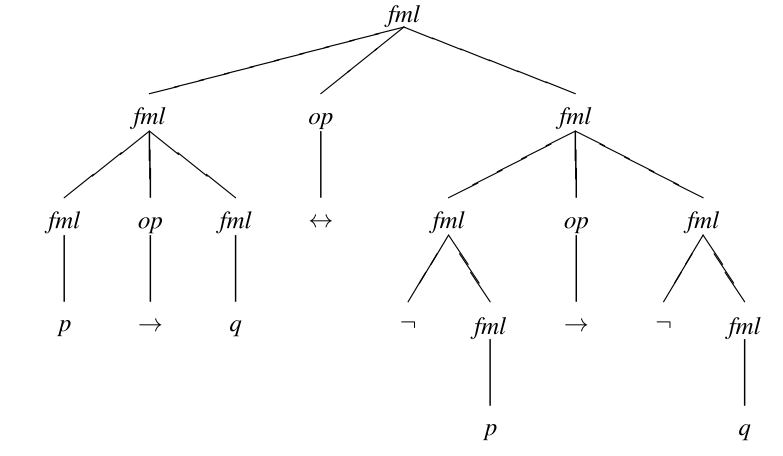
\includegraphics[width=1.0\textwidth]{A3}					
% \caption[Ableitungsbaum für p $\rightarrow$   q $\leftrightarrow$ $\neg$p $\rightarrow$  $\neg$q]{Derivation tree for p $\rightarrow$   q $\leftrightarrow$ $\neg$p $\rightarrow$  $\neg$q}					
% \label{Abb. 2.2} 
%\end{figure}
%
%\begin{align*}
%&fml\\
%&fml \  op \ fml\\
%&fml \leftrightarrow fml\\
%&fml \  op \  fml \leftrightarrow fml\\
%&fml \rightarrow fml \leftrightarrow fml\\
%&p \rightarrow fml \leftrightarrow fml\\
%&p \rightarrow q \leftrightarrow fml\\
%&p \rightarrow q \leftrightarrow fml  \  op \  fml\\
%&p \rightarrow q \leftrightarrow fml \rightarrow fml\\
%&p \rightarrow q \leftrightarrow \neg fml \rightarrow fml\\
%&p \rightarrow q \leftrightarrow \neg p \rightarrow fml\\
%&p \rightarrow q \leftrightarrow \neg p \rightarrow \neg q
%\end{align*}
%
%
%
%%\begin{figure}[ !h] \centering												
%% 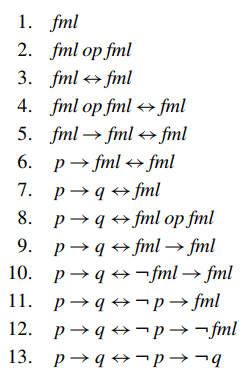
\includegraphics[width=0.3\textwidth]{A0}									
%% \label{Abb. A0}
%%\end{figure}
%
%
%Die in Abschn. \ref{sssec:num1} kann zur Auflösung von Mehrdeutigkeiten verwendet werden. Wir können die Grammatik ändern, um Klammern einzuführen: 
%\begin{align*}
%fml &:: = (\neg \  fml)\\
%fml &:: = (fml \  op \  fml)
%\end{align*}
%und dann die Präzedenz verwenden, um ihre Anzahl zu reduzieren.
%

%	\include{SematikDerAussagenlogik}
%	\section{Erfüllbarkeit und Tautologien}
Grundsätzlich kann man Formeln danach klassifizieren, ob überhaupt passende Belegungen
existieren, die sie wahr oder falsch machen.
\begin{defi} \label{Definition 2.38} \end{defi} 
Eine Formel A heißt: 
\begin{itemize}																					
\item \textit{erfüllbar}, falls sie unter wenigstens einer Belegung wahr ist.
\item \textit{Tautologie}, falls sie für jede passende Belegung wahr ist.
\item \textit{unerfüllbar}, falls es keine passende Belegung wahr gibt.
\end{itemize}
\begin{sa} \label{Satz 2.39} \end{sa}
Eine Formel $A$ ist gültig genau dann wenn $\neg A$ unerfüllbar ist.
%	\section{Semantisches Tableau}
%
%Die Methode der semantischen Tableaus ist eine effiziente Entscheidungsprozedur für Erfüllbarkeit (und Dualität) in der Aussagenlogik.
% 
%Das Prinzip hinter semantischen Tableaus ist sehr einfach: Sucht man nach einem Modell, das die Interpretation erfüllt, indem man die Formel in mehrere Mengen von Atomen und Negationen zerlegt. Eine Menge von Atomen und Negationen von Atomen ist erfüllbar, wenn die Menge kein Atom $p$ und seine Negation $\neg p$ enthält. Die Formel ist erfüllbar, wenn eine dieser Mengen erfüllbar ist. Die Formel ist unerfüllbar, wenn keine Mengen erfüllbar ist d.h seine Negation eine Tautologie. 

Das Prinzip hinter semantischen Tableaus ist sehr einfach: Man sucht nach einem Modell, das die Interpretation erfüllt, indem man die Formel in mehreren Mengen von Literalen zerlegt. Eine Menge von Literalen ist erfüllbar, wenn die Menge kein komplementäres Literalpaar enthält. Die Formel ist erfüllbar, wenn eine dieser Mengen erfüllbar ist. Die Formel ist unerfüllbar, wenn keine Mengen erfüllbar sind, d.h seine Negation eine Tautologie ist.

\begin{defi} \label{Definition 2.57} Literal und komplementäres Literalpaar\cite{Ben-Ari}\end{defi} 
Ein Literal ist ein Atom oder die Negation eines Atoms. Ein Atom ist ein positives Literal und die Negation eines Atoms ist ein negatives Literal. Für jedes Atom $p$ ist $\{p, \neg p\}$ ein komplementäres Literalpaar.

Für jede Formel $A$ ist $\{A, \neg A\}$ ein komplementäres Formelpaar. $A$ ist das Komplement von $\neg A$ und $\neg A$ ist das Komplement von $A$.

\begin{ex} \label{Beispiel 2.58} \end{ex} In der Menge der Literale $ \{ \neg p, q, r, \neg r \} $ sind $q$ und $r$ positive Literale, während $\neg p$ und $\neg r$ negative Literale sind. Die Menge enthält das komplementäre Literalpaar $ \{ r, \neg r \}$.
 
%\begin{bem} \label{Satz 2.60 } Eine Menge von Literalen ist genau dann erfüllbar, wenn sie kein komplementäres Literalpaar enthält.\end{bem}
 
 
%\begin{sa} \label{Satz 2.60 } \end{sa}Eine Menge von Literalen ist genau dann erfüllbar, wenn sie vorhanden ist enthält kein komplementäres Literalpaar.

In der Methode der semantischen Tableaus bezeichnen Mengen von Formeln Knoten eines Baumes, wobei jeder Pfad im Baum die Formeln darstellen, die in einer möglichen Interpretation erfüllt sein müssen.

\begin{defi} \label{Def.Tableau} Konstruktion von semantischen Tableaus\end{defi} 
\begin{itemize}
\item Ein aussagenlogisches Tableau ist ein markierter Baum. Jeder Knoten ist mit einer Menge von Formeln markiert.
\item Die Eingabeformel ist an der Wurzel. 
%\footnote{\url{https://www.ki.informatik.uni-frankfurt.de/lehre/SS2008/AD/folien/ded-fol3.pdf}}
\item Jeder Knoten hat einen oder zwei untergeordnete Knoten, abhängig davon, wie eine Formel, die den Knoten kennzeichnet, zerlegt wird. Dadurch, dass ein Knoten mit $\alpha$-Formel gekennzeichnet wird, hat er nur einen untergeordneten Knoten, ansonsten hat er zwei Knoten. Die Klassifizierung von $\alpha$- und $\beta$-Formeln wird in der Tabelle \ref{Abb. 2.8} definiert.
\item Die Blätter sind durch eine Menge von Literalen markiert.
\item Ein Blatt, das durch eine Menge von Literalen markiert ist, die ein komplementäres Paar von Literalen enthält, ist mit geschlossen ($\times$) markiert
\item Ein Blatt, das durch eine Menge von Literalen markiert ist, die kein komplementäres Paar von Literalen enthält, ist mit offen ($\odot$) markiert. 
\item Ein Tableau ist geschlossen, wenn alle seine Blätter als geschlossen markiert sind. Ansonsten (wenn ein Blatt als offen markiert ist), ist es offen.\cite{Ben-Ari}
\end{itemize}


Abbildung \ref{Abb. 2.7} zeigt semantische Tableaus für die Formeln:

$A = p\wedge (\neg q \vee \neg p)$ und $B = (p \vee q) \wedge  (\neg p \wedge  \neg q)$.

\begin {figure}[h]
\vspace{1cm}
\begin{center}
\definecolor{ududff}{rgb}{0.30196078431372547,0.30196078431372547,1}
\definecolor{uuuuuu}{rgb}{0,0,0}
\begin{tikzpicture}[line cap=round,line join=round,>=triangle 45,x=1cm,y=1cm]
\clip(-13.0,-8.0) rectangle (-2.0,-0.5);
\draw [->,>=stealth,line width=1pt] (-11,-2) -- (-11,-3);
\draw [->,>=stealth,line width=1pt] (-11.5,-4) -- (-12.5,-4.5);
\draw [->,>=stealth,line width=1pt] (-10.5,-4) -- (-9.5,-4.5);
\draw [->,>=stealth,line width=1pt] (-4.5,-2) -- (-4.5,-3);
\draw [->,>=stealth,line width=1pt] (-4.5,-4) -- (-4.5,-5);
\draw [->,>=stealth,line width=1pt] (-5,-6) -- (-6,-6.5);
\draw [->,>=stealth,line width=1pt] (-4,-6) -- (-3,-6.5);
\begin{small}
\draw[color=uuuuuu] (-11,-0.8) node {$\textbf{A}$};
\draw[color=uuuuuu] (-11,-1.5) node {$p \wedge (\neg q \vee \neg p)$};
\draw[color=uuuuuu] (-11,-3.5) node {$p, \neg q \vee \neg p$};
\draw[color=uuuuuu] (-12.5,-5) node {$p,\neg q$};
\draw[color=uuuuuu] (-12.5,-5.5) node {$\odot$};
\draw[color=uuuuuu] (-9.5,-5) node {$p, \neg p$};
\draw[color=uuuuuu] (-9.5,-5.5) node {$\times$};
\draw[color=uuuuuu] (-4.5,-0.8) node {$\textbf{B}$};
\draw[color=uuuuuu] (-4.5,-1.5) node {$(p\vee q)\wedge(\neg p \wedge \neg q)$};
\draw[color=uuuuuu] (-4.5,-3.5) node {$p\vee q, \neg p \wedge \neg q$};
\draw[color=uuuuuu] (-4.5,-5.5) node {$p\vee q, \neg p, \neg q$};
\draw[color=uuuuuu] (-6,-7.0) node {$p,\neg p, \neg q$};
\draw[color=uuuuuu] (-6,-7.5) node {$\times$};
\draw[color=uuuuuu](-3,-7.0) node {$q,\neg p,\neg q$};
\draw[color=uuuuuu] (-3,-7.5) node {$\times$};
\end{small}
\end{tikzpicture}
\end{center}
\caption[Beispiel Konstruktion für semantische Tableaus]{Semantische Tableaus für $A = p\wedge (\neg q \vee \neg p)$ und $B = (p \vee q) \wedge  (\neg p \wedge  \neg q)$}
\label{Abb. 2.7}
\vspace{1cm}
\end{figure}

Die Tableau-Konstruktion ist nicht eindeutig. Abbildung \ref{Abb. 2.6} ist ein weiteres Tableau für die Formel $B$. Die Unterschiede zwischen dem Tableau in der Abbildung \ref{Abb. 2.7} und in der Abbildung \ref{Abb. 2.6} sind, dass in dem ersten Tableau die Belegung für $\neg p \wedge \neg q$ gesucht werden, bevor die für $p \vee q$  gesucht wird. Das erste Tableau enthält weniger Knoten, was zeigt, dass \textit{Konjunktionen vor Disjunktionen} vorzuziehen sind.

\begin {figure}[!h]
\begin{center}
\vspace{1cm}
\definecolor{ududff}{rgb}{0.30196078431372547,0.30196078431372547,1}
\begin{tikzpicture}[line cap=round,line join=round,>=triangle 45,x=1cm,y=1cm]
\clip(-13.5,-8.0) rectangle (-8.0,-1.3);
\draw [->,>=stealth,line width=1pt] (-11,-2) -- (-11,-3);
\draw [->,>=stealth,line width=1pt] (-11.5,-4) -- (-12.5,-4.5);
\draw [->,>=stealth,line width=1pt] (-10.5,-4) -- (-9.5,-4.5);
\draw [->,>=stealth,line width=1pt] (-12.5,-5.5) -- (-12.5,-6.5);
\draw [->,>=stealth,line width=1pt] (-9.5,-5.5) -- (-9.5,-6.5);
\begin{small}
\draw[color=black]  (-11,-1.5) node {$(p \vee q) \wedge(\neg p \wedge \neg q)$};
\draw[color=black]  (-11,-3.5) node {$p \vee q, \neg p \wedge \neg q$};
\draw[color=black]  (-12.5,-5) node {$p,\neg p \wedge \neg q$};
\draw[color=black]  (-9.5,-5) node {$q, \neg p \wedge \neg q$};
\draw[color=black] (-12.5,-7) node {$p, \neg p, \neg q$};
\draw[color=black] (-9.5,-7) node {$q, \neg p \wedge \neg q$};
\draw[color=black] (-12.5,-7.5) node {$\times$};
\draw[color=black] (-9.5,-7.5) node {$\times$};
\end{small}
\end{tikzpicture}
\end{center}
\caption[Ein weiteres Tableau]{Ein weiteres Tableau für $B$}
\label{Abb. 2.6}

\end{figure}

Eine übersichtliche Darstellung der Regeln für die Erstellung eines semantischen Tableaus kann gegeben werden, wenn \textit{Formeln nach ihrem Hauptoperator klassifiziert} werden (Tabelle \ref{Abb. 2.8}). Wenn \textit{die Formel eine Negation ist, berücksichtigt die Klassifizierung sowohl die Negation als auch den Hauptoperator}. \textit{$\alpha$-Formeln sind konjunktiv} und nur erfüllbar, wenn beide Teilformeln $\alpha_1$ und $\alpha_2$ erfüllt sind, während \textit{$\beta$-Formeln disjunktiv sind} und auch dann erfüllt sind, wenn nur eine der Teilformeln $\beta_1$ oder $\beta_2$ erfüllbar ist.

\begin{table}[h]
\footnotesize
	\begin{center}
			\begin{tabular}{lcccclccc}
			\cline{1-4}
			\cline{6-9}
			\textbf{Nr.}&\textbf{$\alpha$}&\textbf{$\alpha_1$}&\textbf{$\alpha_2$}&   &\textbf{Nr.}&\textbf{$\beta$}&\textbf{$\beta_1$}&\textbf{$\beta_2$}  \\
			\cline{1-4} 
			\cline{6-9}
			
			\textbf{a1}&$\neg \neg A_1$&$A_1$&  &   &&&&\\
			
			\textbf{a2}&$A_1 \wedge A_2$&$A_1$&$A_2$&   &\textbf{b1}&$\neg (B_1 \wedge B_2)$&$\neg B_1$&$\neg B_2$\\
			\textbf{a3}&$\neg (A_1 \vee A_2)$&$\neg A_1$&$\neg A_2$&   &\textbf{b2}&$B_1 \vee B_2 $&$B_1$&$B_2$\\
			
			\textbf{a4}&$\neg (A_1 \rightarrow A_2)$& $A_1$ & $\neg A_2$&   &\textbf{b3}&$(B_1 \rightarrow B_2)$&$\neg B_1$&$B_2$  \\
			
			\textbf{a5}&$\neg(A_1 \uparrow A_2)$& $A_1$&$A_2$&   &\textbf{b4}&$B_1 \uparrow B_2$&$\neg B_1$&$\neg B_2$  \\
			
			\textbf{a6}&$A_1 \downarrow A_2$&$\neg A_1$ & $\neg A_2$&   &\textbf{b5}&$\neg (B_1 \downarrow B_2)$&$B_1$&$B_2$  \\
			
			\textbf{a7}&$A_1 \leftrightarrow A_2$& $A_1 \rightarrow A_2$&$A_2 \rightarrow A_1$&   &\textbf{b6}&$\neg (B_1 \leftrightarrow B_2)$&$\neg (B_1 \rightarrow B_2)$&$\neg (B_2 \rightarrow B_1)$\\
			
			\textbf{a8}&$\neg (A_1 \oplus A_2)$&$A_1 \rightarrow A_2$&$A_2 \rightarrow A_1$&   &\textbf{b7}&$B_1 \oplus B_2$&$\neg (B_1 \rightarrow B_2)$&$\neg (B_2 \rightarrow B_1)$\\
			\cline{1-4} 
			\cline{6-9}			
			\end{tabular}
	\end{center}
	\caption[Klassifizierung von $\alpha$- und $\beta$-Formeln]{Klassifizierung von $\alpha$- und $\beta$-Formeln \cite{Ben-Ari}}
	\label{Abb. 2.8}
\end{table}
		
\vspace{0.5cm}\begin{ex} \label{Beispiel 2.63} \end{ex} Die Formel $p \wedge q$ wird als $\alpha$-Formel klassifiziert, weil sie genau dann gilt, wenn sowohl $p$ als auch $q$ wahr sind. Die Formel $\neg(p\wedge q)$ wird als $\beta$-Formel klassifiziert.
Es ist logisch äquivalent zu $\neg p \vee \neg q$ und ist genau dann wahr, wenn entweder $\neg p$ wahr oder $\neg q$ wahr ist.

Der Algorithmus der Tableau-Konstruktion kann wie folgt formuliert werden:
\begin{al}Konstruktion eines semantischen Tableaus \cite{Schaefer}\label{Algorithmus 2.64} \end{al} 
\textit{Eingabe:} Aussagenlogische Formel $A$.\\
\textit{Ausgabe:} Semantisches Tableau mit markierten Blättern
\begin{enumerate}[wide=0em, leftmargin=*, label=\arabic*, itemsep=0pt, parsep=0pt, font=\scriptsize]
\item \textbf{function} Tableau($A$)
\item \tabto{0.cm} Konstruiere einen Baum mit Formel $A$ als Wurzel.
\item \tabto{0.5cm} \textbf{while} es gibt unmarkierte Blätter \textbf{do} 
\item \tabto{0.5cm} Wähle unmarkiertes Blatt $l$
\item \tabto{1cm}\textbf{if}  Blatt $l$ enthält nur Literale then
\item \tabto{1.5cm} \textbf{if} Blatt $l$ enthält komplementäre Literale oder Konstante \textit{false} \textbf{then}
\item \tabto{2cm} Markiere Blatt $l$ als geschlossen mit $\times$ 
\item \tabto{1.5cm} \textbf{else} 
\item \tabto{2cm} Markiere Blatt $l$ als offen mit $\odot$
\item \tabto{1.5cm} \textbf{end if} 
\item \tabto{1cm} \textbf{else if}  Blatt $l$ enthält $\alpha$-Formel then
\item \tabto{1.5cm} Wähle $\alpha$-Formel $\alpha$
\item \label{TableauAl_13} \tabto{1.5cm} Ermittle Formeln $\alpha_1$ und $\alpha_2$ nach Tabelle \ref{Abb. 2.8} 
\item \tabto{1.5cm} Erzeuge Kind $l'$ von $l$
\item \tabto{1.5cm} Beschrifte $l'$ mit Formeln aus $l$
\item \label{TableauAl_16}\tabto{1.5cm} Ersetze dabei $\alpha$ in $l'$ durch Formeln $\alpha_1$  und $\alpha_2$
\item \tabto{1cm} \textbf{else} 
\item \tabto{1.5cm} Wähle  $\beta$-Formel $\beta$
\item \label{TableauAl_19} \tabto{1.5cm} Ermittle Formeln $\beta_1$ und $\beta_2$ nach Tabelle \ref{Abb. 2.8}
\item \tabto{1.5cm} Erzeuge zwei Kinder $l_1$ und $l_2$ von $l$
\item \tabto{1.5cm} Beschrifte $l_1$ mit Formeln aus $l$
\item \tabto{1.5cm} Ersetze dabei $\beta$ in $l_1$ durch $\beta_1$
\item \tabto{1.5cm} Beschrifte $l_2$ mit Formeln aus $l$
\item \label{TableauAl_24}\tabto{1.5cm} Ersetze dabei $\beta$ in $l_2$ durch $\beta_2$
\item \tabto{1cm} \textbf{end if} 
\item \tabto{0.5cm} \textbf{end while}
\item \tabto{0.5cm} \textbf{return}  Semantisches Tableau
\item \textbf{end function}
\end{enumerate}



%\begin{defi} \label{Definition 2.65} \end{defi} Ein Tableau, dessen Konstruktion beendet wurde, ist ein abgeschlossenes Tableau. Ein abgeschlossenes Tableau wird geschlossen, wenn alle seine Blätter als geschlossen markiert sind. Ansonsten (wenn ein Blatt als offen markiert ist), ist es offen.
%\chapter{Frameworks}\label{sec:Frameworks}
Dieses Kapitel befasst sich mit den Frameworks für die Umsetzung:
\begin{itemize}
\item Antlr4 (für die Analyse der Eingabe)
\item Bootstrap (für die Gestaltung der Webanwendung)
\item Google Charts (für die Darstellung des Tableaus) 
\item Jasmine (für das automatisierte Testen)
\end{itemize}

%	\section{Antlr4}\label{sec:Antlr4}
Um die syntaktische Richtigkeit der Benutzereingabeformel zu prüfen und die Formel in einem Baum-Struktur darstellen zu können (\hyperlink{/LF10/}{/LF10/}), wird ANTLR verwendet.

ANTLR ist ein leistungsfähiger Parser-Generator, mit dem man strukturierte Text- oder Binärdateien lesen, verarbeiten, ausführen oder übersetzen kann. Es wird häufig in der Wissenschaft und der Industrie verwendet, um alle möglichen Sprachen, Werkzeuge und Frameworks zu erstellen. ANTLR ist kostenlos und als ``Open Source'' erhältlich.

Die Twitter-Suche verwendet ANTLR für die Abfrageanalyse mit mehr als 2 Milliarden Abfragen pro Tag. Die Sprachen für Hive und Pig und die Data Warehouse- und Analysesysteme für Hadoop verwenden ANTLR. Lex Machina verwendet ANTLR zur Informationsextraktion aus Rechtstexten. Oracle verwendet ANTLR innerhalb der SQL Developer IDE und seiner Migrationstools. Die NetBeans-IDE analysiert C++ mit ANTLR. Die HQL-Sprache im objektrelationalen Hibernate-Mapping-Framework wird mit ANTLR erstellt.\cite{Parr}

Aus einer formellen Sprachbeschreibung, die als Grammatik bezeichnet wird, generiert ANTLR einen Parser für diese Sprache. Ein Parser liest den vom Lexer in einzelne Token zerteilten Strom ein, prüft diese auf syntaktische Richtigkeit und erstellt daraus Symbol-Gruppen mit hierarchischer Struktur. Die Struktur ist oft ein Baum und wird dann abstrakter Syntaxbaum (AST) oder Parse-tree genannt. ANTLR generiert außerdem automatisch Tree-Walker, mit denen Sie die Knoten dieser Bäume aufrufen können, um anwendungsspezifischen Code auszuführen.

%Der wichtigste Unterschied zwischen ANTLR und anderen Parser-Generatoren wie z.B YACC / Bison ist der Typ der Grammatiken, die diese Tools verarbeiten können. YACC / Bison behandeln LALR-Grammatiken, ANTLR behandelt LL-Grammatiken. YACC / Bison erzeugt tabellengesteuerte Parser, was bedeutet, dass die ``Verarbeitungslogik'' in den Daten des Parserprogramms enthalten ist, nicht so sehr in dem Parsercode. ANTLR erzeugt rekursive Descent-Parser, was bedeutet, dass die ``Verarbeitungslogik'' im Parser-Code enthalten ist, da jede Produktionsregel der Grammatik durch eine Funktion im Parser-Code repräsentiert wird. Der Vorteil ist, dass es einfacher ist zu verstehen, was der Parser tut, indem er seinen Code liest. Außerdem sind rekursive Descent-Parser typischerweise schneller als tabellengesteuerte.\footnote{\url{https://stackoverflow.com/questions/212900/advantages-of-antlr-versus-say-lex-yacc-bison}}. 

Um einen AST zu bekommen, muss man:
\begin{itemize}
\item Eine Lexer- und Parsergrammatik definieren.
\item ANTLR aufrufen: Es generiert einen Lexer und einen Parser in einer Zielsprache (z. B. Java, Python, JavaScript)
\item Den generierten Lexer und Parser verwenden: Rufe Lexer und Parser, dann übergebe den Code. Lexer und Parser werden den Code erkennen und einen AST zurückgeben
\end{itemize}

\subsection{Hauptteilen von ANTLR}
ANTLR besteht eigentlich aus zwei Hauptteilen: dem Werkzeug (Antlr-Tool), mit dem der Lexer und Parser erzeugt wird und der Laufzeit, die für die Ausführung benötigt wird. Das Antlr-Tool ist immer gleich, unabhängig davon, auf welche Sprache abgezielt wird. Es ist ein Java-Programm, das nur für Entwickler benötigt wird. Die Laufzeit (Runtime) ist für jede Sprache unterschiedlich und muss sowohl dem Entwickler als auch dem Benutzer zur Verfügung stehen. Die Runtime kann auf der Seite \url{http://www.antlr.org/download/} heruntergeladen werden. 

Die einzige Voraussetzung für das Antlr-Tool ist, dass mindestens Java 1.7 installiert werden muss. Um dieses Antlr-Tool zu installieren, muss die neueste Version von der offiziellen Website, die im Moment \url{http://www.antlr.org/download/antlr-4.7.1-complete.jar} ist, heruntergeladen werden. Die Ausführliche Anleitung zur Installation wird auf der Seite \url{https://github.com/antlr/antlr4/blob/master/doc/getting-started.md} beschrieben.

Wenn man ANTLR verwendet, beginnt man mit dem Schreiben einer Grammatik, einer Datei mit der Erweiterung \textit{.g4}. Diese Grammatik erhält die Regeln der Sprache, die analysiert wird. Dann verwendet man das Antlr-Tool, um die Dateien, die man in seinem Projekt wirklich braucht, zu erstellen,  wie zB. \textit{antlr4 <Optionen> <Grammatik-Datei-Name.g4>}

Es gibt einige wichtige Optionen, die man bei der Ausführung von Antlr-Tool angeben kann. Man kann die Zielsprache angeben, um einen Parser in Python oder JavaScript oder einem anderen Ziel als Java (das ist das Standardziel) zu erstellen.
ANTLR bietet zwei Tree-Walking-Mechanismen in seiner Laufzeitbibliothek: eine Parser-Tree-Listener-Schnittstelle und eine Parser-Tree-Visitor-Schnittstelle \cite{Parr}. Standardmäßig wird nur der Listener generiert. Um den Visitor zu erstellen, kann man die Befehlszeilenoption \textit{-visitor} verwenden. Eine vollständige Liste der Optionen für das Antlr-Tool kann man auf der Seite \url{https://github.com/antlr/antlr4/blob/master/doc/tool-options.md} finden.


\subsection{ANTLR JavaScript target}
Während der Konfiguration von ANTLR in JavaScript gibt es einige Besonderheiten wie folgt:

\begin{itemize}
\item 	Grammatiken im gleichen Ordner wie die JavaScript-Dateien ablegen.
\item	Die Datei mit der Grammatik muss den gleichen Namen wie die Grammatik haben, die am Anfang der Datei angegeben werden muss.
\item	Der entsprechende JavaScript-Parser kann einfach die richtige Option mit dem Antlr-Tool erstellen.

\textit{antlr4 -Dlanguage = JavaScript Grammatik-Datei-Name.g4}

Damit die Manipulationen erleichtert werden, wird in dieser Arbeit eine \textit{.BAT-Datei} \textit{antlr4.bat} verwendet. Die Datei erhält die Kommando
\begin{lstlisting}[language=HTML,basicstyle=\scriptsize]
	antlr4 -Dlanguage=JavaScript -listener -visitor -encoding UTF-8 FormulaGrammar.g4
\end{lstlisting}
um die Parser, Lexer sowie Listener und Visitor für die \textit{FormulaGrammar.g4} in JavaScript zu generieren.

\item	ANTLR kann sowohl mit \textit{node.js} als auch im Browser verwendet werden. Für den Browser muss man webpack oder \textit{require.js} verwenden um zu vermeiden, dass dutzende Dateien manuell importiert werden müssen.

Im Rahmen diese Bachelorarbeit wird \textit{require.js} gewählt. Das Skript wird von Torben Haase zur Verfügung gestellt und ist nicht Bestandteil der ANTLR JavaScript-Runtime. Dieses Skript kann auf der Seite \url{https://github.com/antlr/antlr4/blob/master/runtime/JavaScript/src/lib/require.js\#L65} heruntergeladen werden.
Angenommen hat man im Stammverzeichnis seiner Website sowohl das Verzeichnis ``antlr4'' als auch ein ``lib'' -Verzeichnis mit ``require.js'', muss man die in denn HTML-Header wie folgt einfügen:

\begin{lstlisting}[language=HTML,basicstyle=\scriptsize]
	<script src='lib/require.js'>
	<script>
		var antlr4 = require('antlr4/index');
	</script>
\end{lstlisting}

\item Die generierten  Lexer und Parser in JavaScript kann wie folgt ausgeführt werden:

\begin{lstlisting}[language=JavaScript,basicstyle=\scriptsize ]
	var antlr4 = require('antlr4');
	var MyGrammarLexer = require('./MyGrammarLexer').MyGrammarLexer;
	var MyGrammarParser = require('./MyGrammarParser').MyGrammarParser;
	var MyGrammarListener = require('./MyGrammarListener').MyGrammarListener;

	var input = "your text to parse here"
	var chars = new antlr4.InputStream(input);
	var lexer = new MyGrammarLexer(chars);
	var tokens  = new antlr4.CommonTokenStream(lexer);
	var parser = new MyGrammarParser(tokens);
	parser.buildParseTrees = true;
	var tree = parser.StartRule();
\end{lstlisting}

Dazu sind \textit{MyGrammarLexer.js, MyGrammarParser.js, MyGrammarListener.js} und \textit{MyGrammarVisitor.js} die generierten Dateien für die Grammatik  ``\textit{MyGrammar}'', die eine Regel ``\textit{StartRule}'' enthält.

\item	Wenn man den Syntaxbaum mit einem benutzerdefinierten Listener besuchen möchte, kann man einen benutzerdefinierten Listener wie folgt erstellen:

\begin{lstlisting}[language=JavaScript,basicstyle=\scriptsize]
	MyGrammarListener = function(ParseTreeListener) {
		// some code here
	}
	// some code here
	MyGrammarListener.prototype.enterKey = function(ctx) {};
	MyGrammarListener.prototype.exitKey = function(ctx) {};
	MyGrammarListener.prototype.enterValue = function(ctx) {};
	MyGrammarListener.prototype.exitValue = function(ctx) {};
\end{lstlisting}

Um benutzerdefiniertes Verhalten bereitzustellen, kann man eine Klasse wie folgt erstellen:

\begin{lstlisting}[language=JavaScript,basicstyle=\scriptsize]
	var KeyPrinter = function() {
		MyGrammarListener.call(this); // inherit default listener
		return this;
	};

	// continue inheriting default listener
	KeyPrinter.prototype = Object.create(MyGrammarListener.prototype);
	KeyPrinter.prototype.constructor = KeyPrinter;

	// override default listener behavior
	KeyPrinter.prototype.exitKey = function(ctx) {
	console.log("Oh, a key!");
	};
\end{lstlisting}

Um diesen Listener auszuführen, fügt man dem obigen Code einfach die folgenden Zeilen hinzu:

\begin{lstlisting}[language=JavaScript,basicstyle=\scriptsize]
	...
	tree = parser.StartRule() // only repeated here for reference
	var printer = new KeyPrinter();
	antlr4.tree.ParseTreeWalker.DEFAULT.walk(printer, tree);
\end{lstlisting}

\end{itemize}
Die Ausführliche Anleitung zur JavaScript Konfiguration kann man auf der Seite \url{https://github.com/antlr/antlr4/blob/master/doc/javascript-target.md} lesen. 
%	\section{Bootstrap}
%https://www.internet-exposure.com/blog/standalone-mobile-websites-vs-responsive-design/
Immer mehr Smartphones, Tablets und andere Mobilgeräte werden genutzt, um im Internet zu surfen. Weltweit werden 68 Millionen Google-Suchanfragen pro Stunde auf Mobilgeräten durchgeführt. Laut StatCounter waren im Juli 2018 52,95\% des weltweiten Internetverkehrs auf einem Mobilgerät. Weitere 3,94\% kamen von Tablets \cite{statCounter}. Das bedeutet, dass Mobile Nutzer einen großen Einfluss haben, mit dem man rechnen muss um den langfristigen Erfolg sicherzustellen. Es gibt zwei Optionen zum Erstellen einer für Mobilgeräte optimierten Website. Man kann eine separate mobile Website oder eine Responsive-Website entwickeln.
 
\subsection{Eigenständige mobile Website (Separate mobile Website)}
%Mobile-dedizierte Websites
Separate mobile Websites sind Websites, die speziell für Mobilgeräte entwickelt wurden. Sie leben häufig unter einer separaten URL (z.B. \textit{m.site.de}) und unterscheiden sich von der vollständigen Website. Sie enthalten Funktionen oder Inhalte, die für Mobilgeräte als geeignet erachtet wurden. Häufig sind dies nur einige der auf dem Desktop verfügbaren Komponenten. 
%(muss noch umschreiben)Sie stehen oft im Gegensatz zu Responsive-Websites, die für Mobilgeräte und Desktops in der Regel dieselben Inhalte und Funktionen enthalten, diese jedoch auf Mobilgeräten neu anordnen. 
Eine separate mobile Website bietet Differenzierung von mobilen Inhalten und erstellt ein vollständig mobiles Benutzererlebnis.

%http://todayslocalmedia.com/standalone-mobile-site-vs-mobile-responsive-site/
Das größte Problem mit separaten mobilen Websites besteht darin, dass man zwei separate Websites erstellen und verwalten muss. Wenn man Änderungen an der einen Website vornehmen muss, muss man dieselben Änderungen auf der anderen Website wiederholen. Dies könnte mehr Zeit und Geld kosten. Auch wenn man es auf einer separaten Domain platziert, muss man für eine neue Domain und das Hosting bezahlen. Die Umleitung kann die Ladezeit beeinflussen, was die Absprungrate erhöhen kann, da Besucher ungeduldig sein können.

% Aber der große Nachteil der Erstellung einer separaten Website besteht darin, dass viel mehr Wartung erforderlich ist, um die zwei Versionen (eine für Mobilgeräte und eine für Desktop) einer Website homogen zu halten.

\subsection{Sich anpassendes Design (Responsive-Design)}
Der Begriff Responsive-Design, zuerst von Ethan Marcote im Jahr 2010 geprägt, beschreibt eine Entwicklungstechnik, bei der das Design einer Website automatisch an die Größe der Benutzerbildschirme angepasst wird. Daher kann derselbe Inhalt in einem dreispaltigen Format auf einem Desktop, einem zweispaltigen Format auf einem Tablet und einem einspaltigen Format auf einem Smartphone angezeigt werden. Kurztipp: Man kann feststellen, ob eine Website ``responsive'' ist, indem man das Browserfenster manuell vergrößert oder verkleinert.

Responsive-Design liefert für jede Seite unabhängig vom Gerät den gleichen Code über eine einzige URL an den Browser. Man muss nicht mehr zwei Versionen einer Website erstellen: eine für Desktop-Computer und eine für mobile Geräte. Da es sich nur um eine Website handelt, ist eine Responsive-Website einfacher und kostengünstiger zu warten. Alle Änderungen, die man vornimmt, sind sowohl in der mobilen Version als auch in der Desktop Version sichtbar. Außerdem sind Responsive-Websites oft einfacher zu implementieren und weniger kompliziert in Bezug auf die Konfiguration für Suchmaschinen.

%https://alphadigital.com.au/blog/responsive-adaptive-dedicated-mobile-sites/
Es gibt jedoch auch Nachteile, die mit Responsive-Design einhergehen. Da eine Responsive-Website als eine einzelne Entität codiert ist (im Gegensatz zu einer Desktop-Website und dann einer separaten mobilen Website), müssen alle Seitenressourcen und Code für jeden Besuch des Benutzers heruntergeladen werden, unabhängig von der Bildschirmgröße oder Gerät, das sie besuchen. In mobilen Versionen von Responsive-Website werden häufig bestimmte Elemente nicht angezeigt, um Webseiten oder Abschnitte benutzerfreundlicher zu machen. Diese Elemente müssen jedoch ``unsichtbar'' geladen werden. Dies bedeutet, dass die Webseiten mit dem Responsive-Design wahrscheinlich langsamer geladen werden.

%Sodass ist das Responsive-Design wartungsfreundlich, 
%Dagegen hat Responsive-Design auch einige Nachteile wie bei große Seiten, die für den Desktop geeignet sind, werden möglicherweise nur langsam auf Mobilgeräte geladen. Außerdem könne die Elemente können sich bewegen, daher bietet Responsive-Design keine vollständig mobile Benutzererfahrung.

%Der grafische Aufbau einer Responsive-Website erfolgt anhand der Anforderungen des jeweiligen Gerätes, mit dem die Website betrachtet wird. Dies betrifft insbesondere die Anordnung und Darstellung einzelner Elemente, wie Navigationen, Seitenspalten und Texte, aber auch die Nutzung unterschiedlicher Eingabemethoden von Maus (klicken, überfahren) oder Touchscreen (tippen, wischen). Technische Basis hierfür sind die neueren Webstandards HTML5, CSS3 (hier insbesondere die Media Queries) und JavaScript\footnote{\url{https://de.wikipedia.org/wiki/Responsive_Webdesign}}.




%Vorteil
%\begin{itemize}
%\item	Leichter und kostengünstiger zu warten.
%\item	Eine URL für alle Geräte. Keine Notwendigkeit für komplizierte Annotation.
%\item	Keine komplizierte Erkennung und Umleitung von Geräten erforderlich.
%\item	Uniform & nahtlose = gute UX.
%\item	Fülle der zu verwendenden Vorlagen.
%\item	SEO freundlich.
%\item	Oft einfacher zu implementieren
%\end{itemize}

%Nachteil
%\begin{itemize}
%\item	Große Seiten, die für den Desktop geeignet sind, werden möglicherweise nur langsam auf Mobilgeräte geladen.
%\item	Bietet keine vollständig mobile Benutzererfahrung.
%\item	Weniger Bildschirmgröße Design-Steuerelement.
%\item	Elemente können sich bewegen
%\item	Anzeigen auf dem Bildschirm verloren.
%\item	Längere mobile Downloadzeiten
%\end{itemize}

\subsection{Mobile-first}
Außerdem gibt es noch die Begriffe ``Desktop-First'' und ``Mobile-First''. Während Responsive-Design eine Entwicklungstechnik ist, sind Desktop-First und Mobile-First die Design-Strategien\cite{Gonzalo}.

Desktop-First ist ein Konzept im Responsive-Design bei dem als erstes die Website für die Desktop-Darstellung entwickelt wird. Für kleinere Displays wird die Seite im Nachhinein angepasst\cite{kulturbanause}.\\
Mobile-First, eine Idee von Luke Wroblewski, ist ein Trend in der Website-Entwicklung, bei der das Entwerfen einer Website für Smartphones, Tablets und mobilen Geräte Vorrang vor der Desktop-Version hat. Mit Mobile-First wird ein Webdesigner angesichts der Einschränkungen einer mobilen Plattform (kleiner Bildschirm, langsamere Prozessoren) eine Website erstellen und dann die Website entweder für die Desktop Nutzung kopieren oder verbessern.

\begin{figure}[ !h] \centering
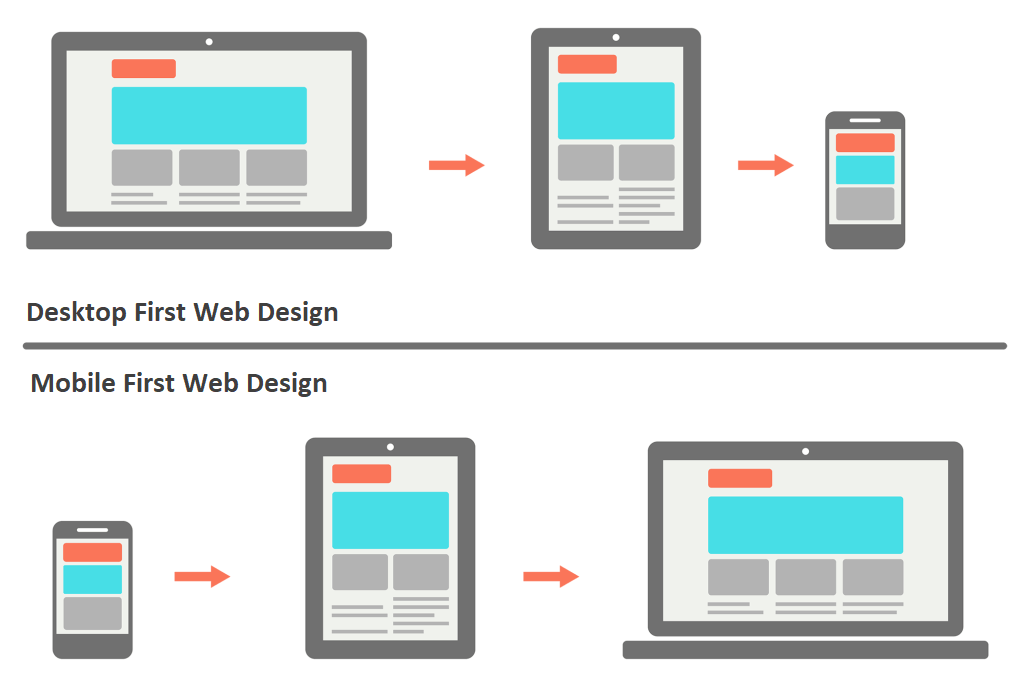
\includegraphics[width=1.0\textwidth]{DesktopMobileFirst}
\caption[Desktop-First und Mobile-First]{Desktop-First und Mobile-First\\ Quelle: \url{http://fredericgonzalo.com/en/2017/03/01/understanding-the-difference-between-mobile-first-adaptive-and-responsive-design/}}\label{fig:DesktopMobileFirst}
\end{figure}

\subsection{Bootstrap} \label{Bootstrap}
Aufgrund der Unterstützung für die Informatik Studierenden (\hyperlink{/LE10/}{/LE10/}und \hyperlink{/LE40/}{/LE40/}), die den Laptop fast täglich verwenden müssen, den Wartungsaufwand und die Implementierungskomplexität, wird eine Responsive-Website mit ``Laptop-First'' Strategie (Bildschirmgröße $\geq$ 768 px) gewählt. Um eine Responsive-Website schneller und einfacher gestalten zu können, wird Bootstrap verwendet.

Bootstrap ist ein beliebtes, kostenloses HTML-, CSS- und JavaScript-Framework zum Entwickeln von Responsive-Websites mit Priorisierung von Mobilgeräten. Das Framework enthält Responsive-CSS- und -HTML-Vorlagen für Schaltflächen, Tabellen, Navigation, Bildkarussells und andere Elemente, die man auf der Webseite verwenden kann. Es sind einige optionale JavaScript-Plugins verfügbar, die selbst Entwicklern mit lediglich grundlegenden Codierungskenntnissen das Entwickeln großartiger Responsive-Websites ermöglichen. Bootstrap ist mit allen modernen Browsern kompatibel wie (\hyperlink{/LE10/}{Chrome}), Firefox, Internet Explorer, Safari und Opera \cite{bootstrapworld}.

\begin{figure}[ !h] \centering
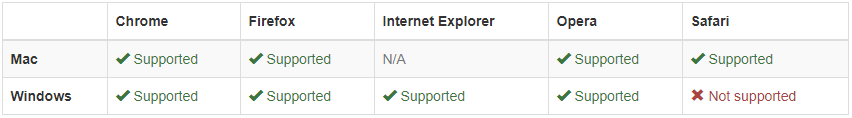
\includegraphics[width=1.0\textwidth]{DesktopBrowsers}
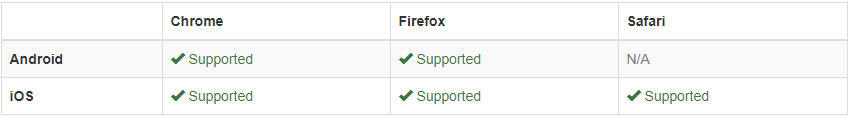
\includegraphics[width=1.0\textwidth]{MobileBrowsers}
\caption[Unterstützte Browsers von Bootstrap]{Unterstützte Browsers von Bootstrap\\ Quelle: \url{https://getbootstrap.com/docs/3.3/getting-started/\# support}}\label{fig:DesktopMobileBrowsers}
\end{figure}

Bootstrap wurde 2010 von Twitter unter dem Namen „Twitter Bootstrap“ entwickelt, mit dem Ziel eine einheitliche Bibliothek für die Gestaltung von Weboberflächen zu schaffen. Das Problem war damals, dass für die Designentwicklung bei Twitter viele verschiedene Bibliotheken verwendet wurden. Das führte zu Inkonsistenzen und einem großen Wartungsaufwand. Bootstrap sollte eine gemeinsame Basis schaffen, mit der alle Mitarbeiter arbeiten konnten, um schnell und einfach Websites zu gestalten.
Im August 2011 entschloss sich Twitter dazu, das Bootstrap Framework als Open Source Projekt zu veröffentlichen. Damit war der Siegeszug dieses ausgezeichneten und leicht zu bedienenden Frontend-Frameworks zur Webdesign-Gestaltung nicht mehr aufzuhalten\cite{bootstrap}.

Um Bootstrap zu verwenden, muss man HTML und CSS nicht gut kennen. Es ist ein Vorteil, wenn man ein Backend-Entwickler ist und einige UI-Änderungen vornehmen kann. 
%Bootstrap ist vollständig anpassbar, man kann wählen, welche Komponenten man verwenden möchte und verwendet eine Variablen-Datei, um noch mehr Farbe und Verhalten zum Anpassung zu bekommen. Alles, was man tun muss, ist es die Seite \url{http://getbootstrap.com/customize/} zu besuchen. Dann wählt man die benötigten Plugins aus und klickt man auf Downloaden. 
%Bootstrap bietet auch eine Möglichkeit, die internen Variablen für fortgeschrittene Benutzer zu überschreiben, aber sie bieten ziemlich ordentliche Standardwerte, so dass man sich darüber keine Gedanken machen sollte, es sei denn, man muss dies tun.

%Bootstrap bietet viele Hilfsklassen, die die Entwicklung einer responsiven Website einfach und schnell machen. Man kann jedes Layout mit fester Breite in ein flüssiges Layout umwandeln, indem man einfach seine übergeordnete \textit{.container} Klasse in \textit{.container-fluid} ändern. Bootstrap verfügt außerdem über die Klassen \textit{.visible}, mit denen man steuern kann, wie seine Section auf Tablets und mobilen Geräten angezeigt werden. Beispiel:
%
%\textit{<div class = ``sichtbarer-xs-block visible-sm-block''> </ div>}
%
%In diesem Fall wird das div als ein Section mit display angezeigt: block nur auf Telefonen und Tablets. Es wird auf dem Desktop versteckt werden.

%Um Bootstrap in einer HTML-Seite zu verwenden, muss lediglich ein fertiges ZIP-Archiv von der Bootstrap-Webseite \url{http://getbootstrap.com/docs/3.3/getting-started/\# download} heruntergeladen werden. 
Bootstrap-Bibliothek kann als ein ZIP-Archiv von der Bootstrap-Webseite \url{http://getbootstrap.com/docs/3.3/getting-started/\# download} heruntergeladen werden. Dieses Archiv enthält bereits fast alle benötigten, in das eigene Projekt einzubindenden Dateien, wie eine Stylesheetdatei mit allen Komponenten, eine JavaScript-Datei mit allen Plugins und auch eine benötigte Icon-Schriftart. Alternativ gibt es auf GitHub noch ein vollständiges, deutlich umfangreicheres ZIP-Archiv für Entwickler herunterzuladen, welches auch Beispiele für typische Webseiten zur bequemen Verwendung als Ausgangsdatei und vieles weitere enthält.

Die Dateien im ZIP-Archiv müssen in das eigene HTML-Dokument/Projekt eingebunden werden. Soll auch mit JavaScript-Komponenten gearbeitet werden, so muss die JavaScript-Datei zusammen mit der jQuery-Bibliothek ebenfalls im HTML-Dokument referenziert werden. Möchte man angepasste Einstellungen für Stil und JavaScript-Funktionalität, besteht die Möglichkeit, fast alle Elemente von Bootstrap auf der Website selbst zu verändern und ein angepasstes Paket herunterzuladen. Schließlich kann man Bootstrap auch lokal, seinen Bedürfnissen entsprechend, vom Standard abweichend kompilieren.

Das folgende Beispiel verdeutlicht die Funktionsweise. Der HTML-Quellcode definiert ein einfaches Suchformular sowie eine Ergebnisliste in Form einer Tabelle. Die Seite besteht aus regulären, semantisch verwendeten HTML5-Elementen sowie einigen zusätzlichen CSS-Klassenangaben entsprechend der Bootstrap-Dokumentation \cite{bootstrapwiki}.

\lstinputlisting[language=HTML, caption=Bootstrap Beispiel, basicstyle=\scriptsize]{ex.html}
%\begin{lstlisting}[language=HTML, caption=Bootstrap Beispiel]
%<!DOCTYPE html>
%<html>
%
%  <head>
%    <title>Bootstrap Beispiel</title>
%
%    <!-- Einbinden des Bootstrap-Stylesheets -->
%    <link rel="stylesheet" href="https://ajax.aspnetcdn.com/ajax/bootstrap/3.3.7/css/bootstrap.min.css">
%
%    <!-- optional: Einbinden der jQuery-Bibliothek -->
%    <script src="https://ajax.aspnetcdn.com/ajax/jQuery/jquery-1.12.4.min.js"></script>
%
%    <!-- optional: Einbinden der Bootstrap-JavaScript-Plugins -->
%    <script src="https://ajax.aspnetcdn.com/ajax/bootstrap/3.3.7/bootstrap.min.js"></script>
%  </head>
%
%  <body>
%    <section class="container">
%      <h1>Suche</h1>
%      <p>Beispiel für ein einfaches Suchformular.</p>
%      <!-- Suchformular mit Eingabefeld und Button -->
%      <form class="well form-search">
%        <input type="text" class="input-medium search-query"/>
%        <button type="submit" class="btn btn-primary">Search</button>
%      </form>
%
%      <h2>Ergebnisse</h2>
%      <!-- Tabelle mit abwechselnder Zellenhintergrundfarbe und Ausserrahmen -->
%      <table class="table table-striped table-bordered">
%     
%      </table>
%    </section>
%  </body>
%
%</html>
%\end{lstlisting}

\textbf{Grid System}

Das Grid-System ist eines der wichtigsten Konzepte in Bootstrap, das beschreibt, wie man Komponenten auf der Oberfläche positionieren und wie man eine Responsive-Website implementieren kann. Im Grid-System ist das Layout der Seite in verschiedene Zeilen aufgeteilt. Jede Zeile hat maximal 12 Spalten (möglicherweise weniger). Basierend auf der Breite des Anzeigegerätetyps kann man verschiedene CSS-Klassen verwenden, um die Anzahl der Anzeigespalten anzupassen. Zum Beispiel hat man eine Webseite, die das Grid Layout System wie folgt verwendet:  

\begin{figure}[ !h] \centering
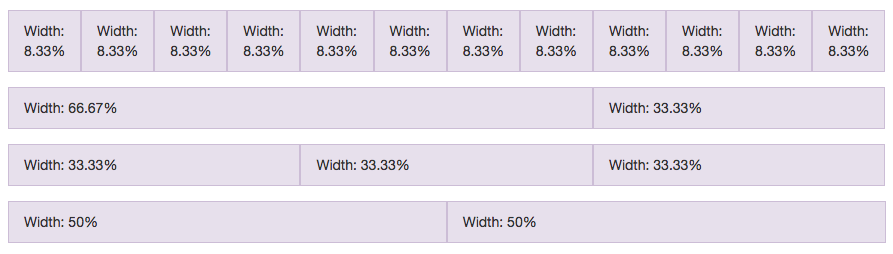
\includegraphics[width=1.0\textwidth]{BootstrapGridSystem}
\caption[Beispiel Grid System]{Beispiel Grid System}\label{fig:BootstrapGridSystem}
\end{figure}

Die Abbildung \ref{fig:BootstrapGridSystem} hat vier verschiedene Zeilen, wobei jede Zeile eine andere Anzahl von Spalten hat, beispielsweise die erste Zeile hat 12 Spalten. Die CSS-Klasse, die auf die Spalte angewendet wird, ist in fünf verschiedene Kategorien unterteilt (Tabelle \ref{tab:BootstrapGridSystem}). 

\begin{table}[h]
\footnotesize
	\begin{center}
			\begin{tabular}{|l|c|c|c|c|c|}
			\hline
			&\textbf{Extra klein}&\textbf{Klein}&\textbf{Medium}&\textbf{Groß}&\textbf{Extragroß}\\
			& <576px & $\geq$ 576px & $\geq$ 768px&$\geq$ 992px &$\geq$ 1200px\\
			\hline
			\textbf{Maximale }&Keine&540px&120px&960px&1140px\\
			\textbf{Behäterbreite}&(automatisch)&&&&\\
			\hline
			\textbf{Klassenpräfix}&.col-&.col-sm-&.col-md-&.col-lg-&.col-xl-\\
			\hline
			\textbf{Anzahl der Spalten}&\multicolumn{5}{|c|}{12}\\
			\hline
			\textbf{Stegbreite}&\multicolumn{5}{|c|}{30px(15px auf jeder Seite einer Spalte)}\\
			\hline
			\textbf{Nestbar}&\multicolumn{5}{|c|}{Ja}\\
			\hline
			\textbf{Spaltenbestellung}&\multicolumn{5}{|c|}{Ja}\\
			\hline
			\end{tabular}
	\end{center}
	\caption[Rasteroptionen im Bootstrap-Framework]{Rasteroptionen\\Quelle: https://getbootstrap.com/docs/4.1/layout/grid/}
	\label{tab:BootstrapGridSystem}
\end{table}		

Wenn es nur 1 Block \textit{<div class=``col-md''> </div>} und keine Spaltennummer gibt, ist der Standardwert 12 Spalten (voller Block von Containern). Wenn man 3 Blöcke \textit{<div class=``col-md''> </div>} hat, werden die Blöcke automatisch ebenso wie \textit{<div class=``col-md-4''> </div>} unterteilt. Die Bildschirme, die größer als den verwendeten Bildschirm sind, ändern sich nicht. Die kleineren Bildschirme werden automatisch auf \textit{col-12} (eine Spalte pro Zeile) umgeschaltet, wenn keine andere Anpassung vorgenommen wird. Das folgende Beispiel verdeutlicht die Funktionsweise des Grid System.

Zuerst fügt man dieses Meta-Tag dem Head-Tag hinzu.
\begin{lstlisting}[language=HTML, basicstyle=\scriptsize]
<meta name="viewport" content="width=device-width, initial-scale=1.0">
\end{lstlisting}	
Und das Body-Tag ist wie folgt:
\begin{lstlisting}[language=HTML, caption= Beispiel Grid System,basicstyle=\scriptsize]
<div class="container" style="background-color: grey; margin-bottom: 50px;">
   <div class="row">
      <div class="col-md-4 col-sm-6">
         <div class="block"></div>
      </div>
      <div class="col-md-8 col-sm-6">
         <div class="block"></div>
      </div>
   </div>
</div>
\end{lstlisting}
Ergebnisse des Laufs des obigen Codes:
\begin{itemize}
\item Wenn die Bildschirmbreite größer als 768px ist, wird jede Zeile in zwei Spalten aufgeteilt: Eine Spalte belegt 33,33 \% der Bildschirmbreite und eine Spalte belegt 66,67 \% der Bildschirmbreite.
\item  Wenn die Bildschirmbreite weniger als 768px ist, wird jede Zeile in zwei Spalten aufgeteilt: Jede Spalte belegt 50\% der Bildschirmbreite.
\item Wenn die Bildschirmbreite weniger als 576px ist, hat jede Zeile nur eine Spalte.
\end{itemize}

Die Dokumentation von Bootstrap ist essentiell. Bootstrap hat eine umfangreiche Dokumentation inklusive Demos, die auch für Anfänger in dem Bereich leicht nachvollziehbar sind und bis hin zu den komplexesten Elementen alles für den Nutzer zugänglich macht. Unter \url{http://getbootstrap.com/getting-started/\# template} kann man eine grundlegende Vorlage und eine Reihe von Beispielen für unterschiedliche Bedürfnisse \url{http://getbootstrap.com/getting-started/\# examples} herunterladen. Man kann einfach das Bootstrap-Repository herunterladen, in den Ordner \textit{docs / examples} gehen, das gewünschte Beispiel kopieren / einfügen und daran arbeiten.
%https://www.htmlgoodies.com/html5/markup/10-common-uses-of-bootstrap.html


%1. Zunächst ist Bootstrap das beliebteste Framework zum Erstellen von Layouts. Hier sind einige zusätzliche Gründe Bootstrap zu verwenden:
%
%Das reaktionsschnelle CSS von Bootstrap passt sich an Telefone, Tablets und Desktops an
%Mobile-First-Styles sind Teil des Frameworks
%Bootstrap ist mit allen modernen Browsern kompatibel (Chrome, Firefox, Internet Explorer, Safari und Opera).
%2. Bootstrap hat eine große Community und freundlichen Support. Für Ressourcen besuchen Sie:
%Schau dir den Bootstrap Blog an.
%Sie können mit Bootstrappern mit IRC im irc.freenode.net Server im ## bootstrap channel chatten.
%Schaut euch an, was die Leute mit Bootstrap auf der Bootstrap Expo machen.
%3. Bootstrap ist einfach einzurichten und ein funktionierendes Layout in weniger als einer Stunde zu erstellen
%
%Sie haben eine grundlegende Vorlage unter http://getbootstrap.com/getting-started/#template und eine Reihe von Beispielen für unterschiedliche Bedürfnisse (http://getbootstrap.com/getting-started/#examples). Sie können einfach das Bootstrap-Repository herunterladen, in den Ordner docs / examples gehen, das gewünschte Beispiel kopieren / einfügen und daran arbeiten.
%
%4. Sie müssen HTML und CSS nicht gut kennen, um Bootstrap zu verwenden, es ist ein Vorteil, wenn Sie ein Backend-Entwickler sind und einige UI-Änderungen vornehmen müssen.
%
%5. Es ist vollständig anpassbar, ich kann wählen, welche Komponenten ich verwenden möchte und verwenden Sie Variablen-Datei, um noch mehr Farbe und Verhalten Anpassung zu bekommen.
%
%Alles, was Sie tun müssen, ist http://getbootstrap.com/customize/, wählen Sie die benötigten Plugins aus und klicken Sie auf Download. Bootstrap bietet auch eine Möglichkeit, die internen Variablen für fortgeschrittene Benutzer zu überschreiben, aber sie bieten ziemlich ordentliche Standardwerte, so dass Sie sich darüber keine Gedanken machen sollten, es sei denn, Sie müssen dies tun.
%
%6. Wenn Sie die Bootstrap-Version aktualisieren, werden Sie nicht viele Fehler sehen, da sich das Kernteam um die Abwärtskompatibilität kümmert.
%
%7. Ihre Dokumentation ist großartig! Hier sind einige Ressourcen zum Auschecken:
%
%Bootstrap 3 Tutorial
%Code Academy: Bootstrap
%Webdesign-Tutorials: Bootstrap
%8. Bootstrap bietet viele Hilfsklassen, die die Entwicklung einer responsiven Website einfach und schnell machen.
%
%Sie können jedes Layout mit fester Breite in ein flüssiges Layout umwandeln, indem Sie einfach Ihre übergeordnete .container-Klasse in .container-fluid ändern.
%
%Bootstrap verfügt außerdem über die Klassen .visible - * - *, mit denen Sie steuern können, wie Ihre Abschnitte auf Tablets und mobilen Geräten angezeigt werden. Beispiel:
%
%<div class = "sichtbarer-xs-block visible-sm-block"> </ div>
%
%In diesem Fall wird das div als ein Abschnitt mit display angezeigt: block nur auf Telefonen und Tablets. Es wird auf dem Desktop versteckt werden.
%
%9. Bootstrap-Komponenten sind gut in das Ökosystem der beliebten JS MVC Frameworks wie Angular übernommen. Bootstrap bietet mehrere Möglichkeiten, es in Ihr Projekt einzubinden:
%
%Benutzung der Laube:
%
%Bower installieren Bootstrap
%
%Verwenden von npm:
%
%npm install bootstrap
%
%Und einfach ein Skript-Tag mit der URL hinzufügen, um Source auf CDN zu laden.
%
%Wir haben auch ui-bootstrap für Angular.js und react-bootstrap für React. Sie können sie auch über Bower und Npm installieren. Um zum Beispiel ein Kollaps-Element zu erstellen, müssen Sie nur ein ähnliches Markup erstellen:
%
%<div uib-collapse = "isCollapsed">
%
%<div class = "well well-lg">
%
%Inhalt des Einsturzes
%
%</ div>
%
%</ div>
%
%Anstatt eine Menge jQuery-Konfiguration zu machen, wie Sie es normalerweise tun würden.
%
%10. Bootstrap löst viele browserübergreifende Probleme auf und Sie müssen sich nicht ständig darum kümmern.
%
%Hinweis: Bootstrap wurde für die Verwendung mit den neuesten Desktop- und mobilen Browsern entwickelt. Dies bedeutet, dass die Anzeigen in älteren Browsern möglicherweise anders aussehen und möglicherweise anders gerendert werden, obwohl die Anzeigen gemäß der Dokumentation voll funktionsfähig sein sollten.
%
%Hier sind ein paar Screenshots zur Browserkompatibilität.







%Note
%https://www.nngroup.com/articles/mobile-vs-responsive/
%\url{https://www.clickseed.com/responsive-design-vs-separate-mobile-site-vs-dynamic-serving/}
%\url{https://www.interaction-design.org/literature/article/adaptive-vs-responsive-design}
%	\section{Google chart tools}
Um den Tableau zu visualisieren, braucht man ein Werkzeug, das einfach zu bedienen und kostenlos ist. Mit dieser Anforderungen ist Google Charts ein guter Kandidat.

%https://reviews.financesonline.com/p/google-chart-tools/
Google chart tools \cite{googleCharts}(Google Charts, unterscheidet sich von dem Google Chart API) ist ein interaktiver Webservice \cite{googleChartswiki}, mit dem Benutzer ihre Daten auf ihrer Website über einfache oder attraktive Visualisierungen anzeigen können. Das Werkzeug wird häufig mit einem einfachen JavaScript verwendet, das auf der Webseite eingebettet ist. Mit Google Charts können Benutzer die einfachen Diagramme wie Liniendiagramme bis hin zu komplexen Diagrammen wie Baumdiagramme, erstellen. 

Neben dem standardmäßigen Google-Design werden den Nutzern auch zahlreiche Anpassungsoptionen für ihre Diagramme zur Verfügung gestellt. Das Werkzeug ist recht einfach zu bedienen, da Benutzer nur die Anwendung einbetten, die Google Chart-Bibliotheken laden und die zu charternden Daten eingeben müssen. Nach ein paar Anpassungen und der Zuweisung einer ID kann das Diagramm auf der Webseite aktiviert werden.

Google Charts ist nicht nur kostenlos, sondern auch eine benutzerfreundliche Anwendung. Mit ein wenig JavaScript-Kenntnissen kann man komplizierteste Diagramme und Grafiken erstellen. Die Anpassungsoptionen sind auch ein weiterer erwähnenswerter Vorteil. Diagramme können mit Farben, Linien, Überlagerungen, Punkten usw. angepasst und optimiert werden, damit sie sich leicht an die Schnittstelle der Webseite anpassen. Es gibt eine großartige Dokumentation von Google, die  unter der Seite \url{https://developers.google.com/chart/interactive/docs/} nachgeschlagen werden kann.

%https://www.moesif.com/blog/technical/visualization/How-to-Choose-the-Best-Javascript-Data-Visualization-Library/
Gegen die Verwendung von Google Charts spricht zum einen, dass eine Netzwerkverbindung erforderlich ist. Außerdem ist es durch Google den Benutzern nicht gestattet, den Code selbst zu speichern oder zu hosten. Diese Einschränkungen haben jedoch keinen Einfluss auf die Anforderungen der Tableau-Anwendung.
%Und obwohl Google Charts zwar kostenlos ist, ist es aber keine Open Source-Version, es gelten die Google API-Nutzungsbedingungen. 

\subsection{Organigramm}\label{Organigramm}
Da die Struktur von Tableau ein Baum ist, eignet sich das Organigramm von Google Charts gut zur Visualisierung eines Tableaus.

Organigramme sind ein Diagramm einer Knotenhierarchie, die häufig verwendet wird, um übergeordnete / untergeordnete Beziehungen in einer Organisation darzustellen. Eine Baumfamilie ist eine Art Organigramm\cite{orgCharts}.
Der folgenden HTML-Quellcode definiert ein einfaches Organigramme \cite{orgCharts}.

\lstinputlisting[language=JavaScript, caption=Organigramme Beispiel,basicstyle=\scriptsize]{googlecharts_organization_chart.htm}

Zuerst muss man den Loader selbst laden, was in einem separaten \textit{script}-Tag mit erfolgt: 
\begin{lstlisting}[language=HTML,basicstyle=\scriptsize]
	src="https://www.gstatic.com/charts/loader.js"
\end{lstlisting} 
Dieses Tag kann sich entweder im ``head'' oder ``body'' des Dokuments befinden oder dynamisch in das Dokument eingefügt werden. %, während es geladen wird oder nachdem das Laden abgeschlossen wurde.\\
Nachdem der Loader geladen wurde, kann man \textit{google.charts.load} abrufen. 
%Wo man es aufruft, kann es sich in einem script Tag im head oder body des Dokuments befinden, und man kann es aufrufen, während das Dokument noch geladen wird oder zu einem beliebigen Zeitpunkt nach dem Laden.\\
Ab Version 45 kann man \textit{google.charts.load} mehr als einmal abrufen, um weitere Pakete zu laden, aber wenn man dies tut, muss man jedes Mal dieselbe Versionsnummer und dieselbe Spracheinstellung angeben.\\

\begin{lstlisting}[language=JavaScript,basicstyle=\scriptsize]
google.charts.load('current', {packages:"orgchar"]});
\end{lstlisting}

Das erste Argument des \textit{google.charts.load} ist der Name oder die Nummer der Version als String. 
%Zu diesem Zeitpunkt gibt es nur zwei spezielle Versionsnamen und mehrere eingefrorene Versionen.
Wenn man  \textit{current} angibt, wird dadurch die neueste offizielle Version von Google Charts geladen. 
%Wenn man den Kandidaten für das nächste Release testen möchten, verwenden Sie 'upcoming'stattdessen.
Der zweite Parameter des \textit{google.charts.load} ist ein Objekt zum Festlegen von Einstellungen wie Pakete, Sprache, Rückrufen... In dem obigen Beispiel ist \textit{orgchar} der Paketname.

Bevor man eines der von \textit{google.charts.load} geladenen Pakete verwenden kann, muss man warten, bis das Laden beendet ist. 
%Es reicht nicht aus, nur auf das Laden des Dokuments zu warten.
Da es einige Zeit dauern kann, bis das Laden beendet ist, muss man eine Rückruffunktion registrieren. Es gibt zwei Möglichkeiten, dies zu tun. Man gibt entweder eine callback Einstellung in dem \textit{google.charts.load} an oder ruft \textit{setOnLoadCallback} mit einer Funktion (z.B \textit{drawChart()}) als Argument auf.


%Beachtet man, dass man eine Funktionsdefinition bereitstellen muss, anstatt die Funktion aufzurufen. Die angegebene Funktion kann entweder eine benannte Funktion oder eine anonyme Funktion sein. Wenn die Pakete geladen sind, wird diese Callback-Funktion ohne Argumente aufgerufen. Das Ladeprogramm wartet auch auf das Laden des Dokuments, bevor es den Rückruf aufruft.
%
%\begin{lstlisting}[language=HTML, caption=Bootstrap Beispiel]
%google.charts.setOnLoadCallback ( ZeichenChart1 ); 
%  google.charts.setOnLoadCallback ( ZeichenChart2 ); 
%  // ODER 
%  google.charts.setOnLoadCallback ( 
%    function () {// Anonyme Funktion, die drawChart1 und drawChart2 
%         aufruft drawChart1 (); 
%         drawChart2 (); 
%      } );
%\end{lstlisting}


%Wenn man mehr als ein Diagramm zeichnen möchte, kann man entweder mehrere Callback-Funktionen registrieren oder diese zu einer Funktion zusammenfassen.
 
%Wenn man mehrere Diagramme auf einer Webseite zeichnen möchte, fügt man folgenden Code auf \textit{<head>} der Seite hinzu:
%\begin{itemize}
%\item	Ladet man alle von den Diagrammen benötigten Pakete in einem einzigen Aufruf nach \textit{google.charts.load()}.
%\item	Für jede Tabelle auf der Seite, fügt man einen Anruf \textit{google.charts.setOnLoadCallback()} mit dem Rückruf, der das Diagramm als Eingabe zeichnet.
%\end{itemize}
%Wenn man mehrere Diagramme für die gleichen Daten zeichnen möchte, ist es möglicherweise einfacher, einen einzelnen Rückruf für beide Diagramme zu schreiben.

%Vorbereiten die Daten
\subsection{DataTable}
Alle Diagramme benötigen Daten. Google Chart Tools-Diagramme erfordern das Umbrechen von Daten in eine JavaScript-Klasse namens \textit{google.} \textit{visualization.DataTable}. Diese Klasse ist in der Google Visualization-Bibliothek definiert, die man zuvor geladen hat.

Die Organigramm erfordert eine \textit{DataTable} mit drei Spalten, wobei jede Zeile einen Knoten im Organigramm darstellt. Hier sind die drei Spalten:
\begin{itemize}
\item	Spalte 0 : Die Knoten-ID. Es sollte unter allen Knoten \textit{eindeutig} sein und beliebige Zeichen einschließlich Leerzeichen enthalten. Dies wird auf dem Knoten angezeigt. Man kann einen formatierten Wert angeben, der stattdessen im Diagramm angezeigt wird. Der unformatierte Wert wird jedoch weiterhin als ID verwendet.
\item 	Spalte 1(optional): Die ID des übergeordneten Knotens. 
\item	Spalte 2(optional): Tooltip-Text, der angezeigt wird, wenn ein Benutzer den Mauszeiger über diesen Knoten bewegt.
\end{itemize}
Jeder Knoten kann keinen oder einen übergeordneten Knoten und keinen oder mehrere untergeordnete Knoten haben.

\subsection{Zeichnen des Diagramms}
Der letzte Schritt ist das Zeichnen des Diagramms. Zuerst muss man eine Instanz der Diagrammklasse, die man verwenden möchte, instanziieren und dann muss man \textit{draw()} aufrufen.
Jeder Diagrammtyp basiert auf einer anderen Klasse, die in der Diagrammdokumentation aufgeführt ist, z.B. basiert das Organigramm auf der \textit{google.visualization.OrgChart}. 

\begin{lstlisting}[language=JavaScript,basicstyle=\scriptsize]
var chart = new google.visualization.OrgChart(document.getElementById('chart_div'));
\end{lstlisting}

Nachdem man seine Daten und Optionen vorbereitet hat, kann man das Diagramm zeichnen. Die Seite muss ein HTML-Element (normalerweise ein \textit{<div>}) enthalten, um das Diagramm zu halten. Man muss dem Diagramm einen Verweis auf dieses Element übergeben, also weist man ihm eine ID zu, mit der man einen Verweis \textit{document.getElementById()} abrufen kann. Alles in diesem Element wird beim Zeichnen durch das Diagramm ersetzt. 

Jedes Diagramm unterstützt eine \textit{draw()} \textit{Methode} \cite{drawCharts}, die zwei Werte akzeptiert: ein \textit{DataTable} (oder ein \textit{DataView}) Objekt, das seine Daten enthält, und ein optionales Diagrammoptionsobjekt. Das Optionsobjekt ist nicht erforderlich, und man kann es ignorieren oder \textit{Null} übergeben, um die Standardoptionen des Diagramms zu verwenden.

Nach dem Aufruf \textit{draw()} wird das Diagramm auf der Seite gezeichnet. Man soll die \textit{draw()} Methode jedes Mal aufrufen, wenn man die Daten oder die Optionen ändern und das Diagramm aktualisieren möchte. Die \textit{draw()} Methode ist asynchron, d.h. sie wird sofort zurückgegeben während die zurückgegebene Instanz jedoch möglicherweise nicht sofort verfügbar ist.

%Die \textit{draw()} Methode ist asynchron, dh sie wird sofort zurückgegeben während die zurückgegebene Instanz jedoch möglicherweise nicht sofort verfügbar ist. In vielen Fällen ist das in Ordnung, das Diagramm wird schließlich gezeichnet. Wenn man jedoch Werte in einem Diagramm nach dem Aufruf festlegen oder abrufen möchten \textit{draw()}, muss man darauf warten, dass das Ereignis  ``ready'' ausgelöst wird, wodurch angezeigt wird, dass es ausgefüllt ist. 

Außerdem gibt es noch viele Einstellungsmöglichkeiten wie Farbe oder Größe der Diagramme sowie die Methoden und Events..., die unter der Seite \url{https://developers.google.com/chart/interactive/docs/gallery/orgchart} nachgeschlagen werden.  



%	\include{Jasmin}
%	
%\chapter{Analyse} \label{sec:Analyse}
Dieses Kapitel handelt von der Problemanalyse sowie den Anforderungsdefinitionen der Anwendung.

%	\section{Problemanalyse: Lastenheft}
\begin{enumerate}
\item \textbf{Zielbestimmung}
%Es gibt viele Möglichkeiten, wie zum Beispiel das Wahrheitstafelverfahren oder die Äquivalenzumformung, um zu prüfen, ob eine Formel der Aussagenlogik allgemeingültig ist. Die Wahrheitstabellen sind unpraktikabel, da sie exponentiell wachsen. Die Äquivalenzumformung liefert auch kein Verfahren, das sagt, welche Regel anzuwenden ist. Es gibt auch ein alternatives Verfahren, das die Erfüllbarkeit einer aussagenlogischen Formel überprüft. Ebenso gibt es das sogenannte Tableau-Verfahren. 
Es gibt ein Verfahren, das die Erfüllbarkeit einer aussagenlogischen Formel überprüft, die Tableau-Verfahren genannt wird.
Dazu werden systematische Regeln angewendet und Formeln umgeschrieben. Dieses Verfahren kann auch als Programm implementiert und genutzt werden. Daher soll, um das Lehren und Lernen der Informatikmodule besser zu unterstützen, eine Software entwickelt werden, die vom Nutzer eine aussagenlogische Formel annimmt und prüft, ob diese Formel erfüllbar oder allgemeingültig ist. Das Ergebnis soll mittels eines semantischen Tableaus erstellt und angezeigt werden. Außerdem soll die Anwendung eine ``Schritt für Schritt Lösung''- Funktion, wonach Studierende Schritt für Schritt den Aufbau eines Tableaus folgen können, bieten. Die Software soll als Web-Applikation eingeführt werden.

\item \textbf{Produkteinsatz}

\hypertarget{/LE10/}{/LE10/} Verwendung im Bereich Lehren und Lernen der Informatikmodule.

\hypertarget{/LE20/}{/LE20/} Die Nutzer sollen die Funktionalität über eine Webanwendung nutzen können.	

\hypertarget{/LE30/}{/LE30/} Die Software soll ohne Server und Datenbank funktionieren können.

\hypertarget{/LE40/}{/LE40/} Zielgruppe der Software sind Studierende und die Dozierende.

\item \textbf{Produktfunktionen}

\hypertarget{/LF10/}{/LF10/} Eingabeformel überprüfen und anzeigen
\begin{itemize} 
\item Die Software prüft, ob die Eingabeformel ein wohlgeformter Ausdruck der Aussagenlogik ist, sonst Wiederholung der Eingabe.
\item Die Eingabeformel-Darstellung wird als Baumstruktur erstellt und in dem GUI angezeigt .
\end{itemize}


\hypertarget{/LF20/}{/LF20/} Allgemeingültigkeit überprüfen und Tableau darstellen
\begin{itemize}
\item Die Software erstellt die Negation von der Eingabeformel. 
\item Die Software  mittels Tableau-Verfahren prüft, ob diese Negation erfüllbar ist (/LF30/).
\item Wenn diese Negation nicht erfüllbar ist, ist die Eingabeformel allgemeingültig.
\item Wenn diese Negation erfüllbar ist, ist die Eingabeformel nicht allgemeingültig.
\item Die Tableau-Darstellung wird als Baumstruktur erstellt und in dem GUI angezeigt.
\end{itemize}

\hypertarget{/LF30/}{/LF30/}  Erfüllbarkeit überprüfen und Tableau darstellen
\begin{itemize} 
\item Die Software mittels Tableau-Verfahren prüft, ob Eingabeformel erfüllbar ist
\item Die Tableau-Darstellung wird als Baumstruktur erstellt und in dem GUI angezeigt.
\end{itemize}


\hypertarget{/LF40/}{/LF40/}  Schritt für Schritt Lösung anzeigen
\begin{itemize}
\item Ein Pop-up Fenster von der Schritt für Schritt Lösung wird geöffnet.
\item Durch Anklicken eines Buttons kann das Tableau Stück für Stück dargestellt werden und ein Lösungshinweis für jeden Schritt angezeigt werden.
\end{itemize}

\item \textbf{Produktdaten}
\begin{itemize}
\item keine Produktdaten
\end{itemize}

\item \textbf{Produktleistungen}

/LL10/ Die Funktionen /LF20/ und /LF30/ darf nicht länger als 5 Sekunden Reaktionszeit benötigen

/LL20/ Bei fehlerhaften Eingaben erhält der Nutzer eine Fehlermeldung

/LL30/ Bei fehlerhaften Eingaben muss der Nutzer die Möglichkeit haben, eine Korrektur der Eingaben vorzunehmen.

                                                                                                                                                                                                                                                    
\item \textbf{Qualitätsanforderungen}

\hypertarget{/LQ10/}{/LQ10/} Vollständigkeit: Alle implementierten Funktionen werden benutzt. Alle referenzierten Funktionen werden implementiert.

\item \textbf{Ergänzungen}
\begin{itemize}
\item  Die Software soll zunächst unter \hypertarget{Chrome}{Chrome} laufen, langfristig aber auch unter Firefox und weiteren Browsern. 
\end{itemize}

%\item \textbf{Glossar}
%\begin{itemize}
%\item Reaktionszeit:  Zeitdauer bis eine Funktion ausgeführt ist.
%\end{itemize}
\end{enumerate} 


%	\section{Anforderungsanalyse}
\subsection{Anwendungsfalldiagramm}
\begin{figure}[ !h] \centering
%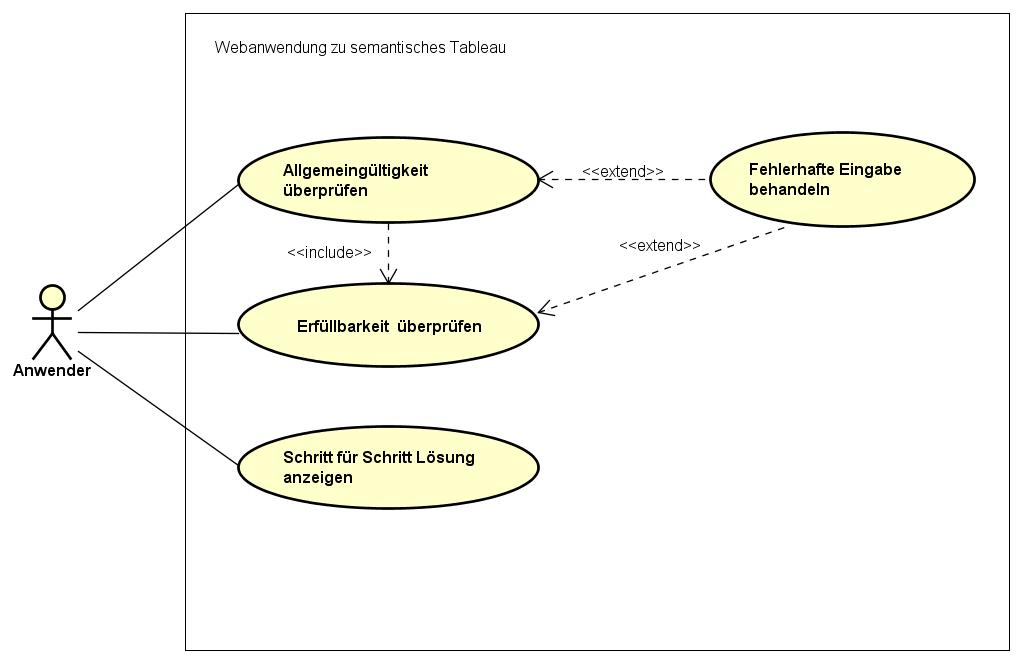
\includegraphics[width=1.0\textwidth,draft=\DraftMode]{UsecaseDiagram}
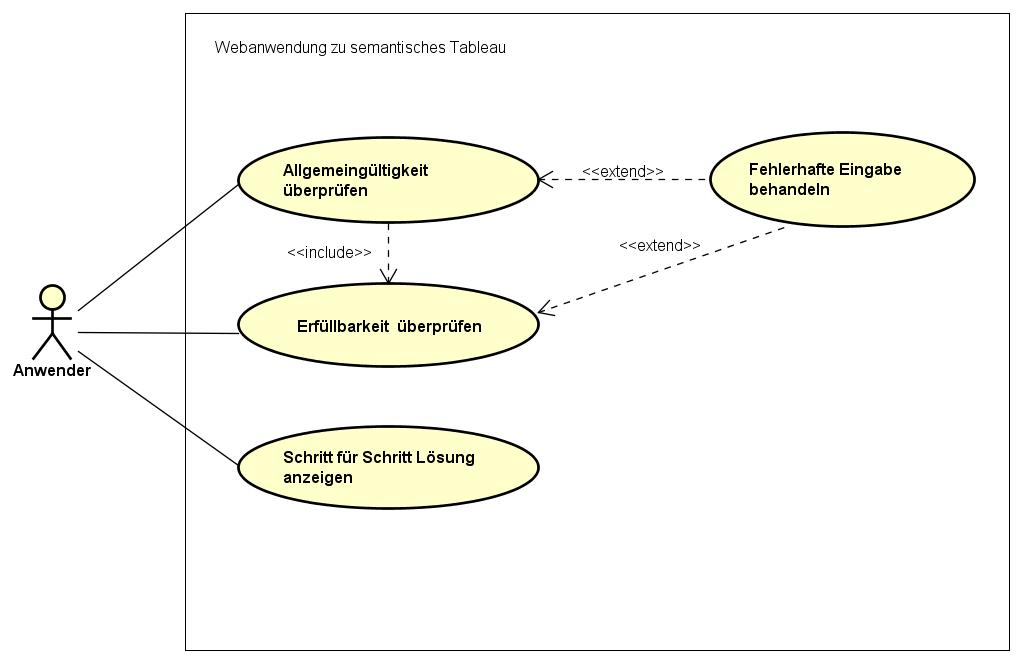
\includegraphics[width=1.0\textwidth]{UsecaseDiagram.jpg}
\caption[Anwendungsfalldiagramm]{Anwendungsfalldiagramm}\label{fig:Anwendungsfalldiagramm}
\end{figure}

\subsection{Anwendungsfallbeschreibung}
\begin{itemize}


%\subsubsection{Anwendungsfall:``Allgemeingültigkeit überprüfen''}
\item \textit{\textbf{Anwendungsfall: ``Allgemeingültigkeit überprüfen''}}

\textbf{Akteure:}

Anwender (initiiert den Anwendungsfall)\\

\textbf{Auslöser:}

Anwender drückt auf ``Tautologie''\\

\textbf{Anfangsbedingungen:}

Der Anwender hat eine Eingabe ins Eingabefeld eingegeben.\\

\textbf{Ereignisfluss:}
\begin{enumerate}
\item Das System prüft, ob die Eingabe ein wohlgeformter Ausdruck der Aussagenlogik ist. 
\item Das System erstellt die Negation der Eingabeformel.
\item Das System zeigt die Darstellung von der Negation der Eingabeformel als Baumstruktur in dem GUI an.
\item Das System initiiert ``Erfüllbarkeit überprüfen'' um zu prüfen, ob die Negation der Eingabeformel erfüllbar ist.
\item Wenn dies erfolgreich ist, erstellt das System das Ergebnis, sodass die Eingabeformel nicht allgemeingültig ist. Wenn nicht, erstellt das System das Ergebnis, sodass die Eingabeformel allgemeingültig ist.
\item Das System zeigt die Darstellung des Tableaus an.
\end{enumerate}

\textbf{Abschlussbedingungen:}

Der Anwender hat entweder das Ergebnis oder eine Systemmeldung über eine fehlerhafte Eingabe erhalten.\\
	
%\subsubsection{Anwendungsfall:``Erfüllbarkeit überprüfen''}
\item \textit{\textbf{Anwendungsfall: ``Erfüllbarkeit überprüfen''}}

\textbf{Akteure:}

Anwender (initiiert den Anwendungsfall)\\

\textbf{Auslöser:}

Anwender drückt auf ``Erfüllbarkeit''\\

\textbf{Anfangsbedingungen:}

Der Anwender hat eine Eingabe ins Eingabefeld eingegeben.\\
 
\textbf{Ereignisfluss:}
\begin{enumerate}
\item Das System prüft, ob die Eingabe ein wohlgeformter Ausdruck der Aussagenlogik ist. 
\item Das System zeigt die Eingabeformel-Darstellung als Baumstruktur in dem GUI an.
\item Das System prüft, ob die Eingabeformel mittels Tableau-Verfahren erfüllbar ist und erstellt das Ergebnis.
\item Das System zeigt die Darstellung des Tableaus an.
\end{enumerate}

\textbf{Abschlussbedingungen:}

Der Anwender hat entweder das Ergebnis oder eine Systemmeldung über eine fehlerhafte Eingabe erhalten.\\

%\subsubsection{Anwendungsfall: ``Schritt für Schritt Lösung auswählen''}
\item \textit{\textbf{Anwendungsfall: ``Schritt für Schritt Lösung anzeigen''}}

\textbf{Akteure:}

Anwender (initiiert den Anwendungsfall)\\

\textbf{Auslöser:}

Anwender drückt auf ``Schritt für Schritt Lösung''\\

\textbf{Anfangsbedingungen:}

Anwender hat ``Erfüllbarkeit'' oder ``Tautologie'' gedrückt.\\

\textbf{Ereignisfluss:}
\begin{enumerate}
\addtolength{\itemindent}{0cm}
\item Das System öffnet ein Pop-up Fenster für die Schritt für Schritt Lösung.
\addtolength{\itemindent}{1cm}
\item  Der Anwender drückt auf ``Nächste Schritt'' um den nächsten Schritt der Lösung anzuzeigen.
\item  Der Anwender drückt auf ``$\times$'' Symbol um das Pop-up Fenster zu schließen.
\addtolength{\itemindent}{0cm}
\end{enumerate}
\begin{enumerate}
  \setcounter{enumi}{3}
 \item Das System schließt das Pop-up Fenster.
\end{enumerate}

\textbf{Abschlussbedingungen:}
Pop-up Fenster ist geschlossen. Der Anwender kann die vorherige Formel nochmal prüfen oder eine neue Formel eingeben.\\

%\textbf{Anwendungsfall:}  "Tableau anzeigen"
%\textbf{Akteure:}
%- System (initiiert den Anwendungsfall)
%-Google Chart Tools (stellt das Tableau dar)
%\textbf{Auslöser:}
%Das System initiiert " Tableau darstellen " zur Darstellung des Tableaus.
%\textbf{Anfangsbedingungen:}
%Das System hat das Tableau erstellt.
%\textbf{Ereignisfluss:}
%1.	Das System prüft, ob die Eingabe ein wohlgeformter Ausdruck der Aussagenlogik ist. 
%2.	Das System prüft, ob die Eingabe Formel mittels Tableau-Verfahren erfüllbar ist und erstellt das Ergebnis.
%3.	Das System initiiert " Tableau darstellen " zur Darstellung des Tableaus.
%\textbf{Abschlussbedingungen:}
%Die Tableau-Darstellung müssen innerhalb von 5 Sekunden bereitgestellt werden können.
%\textbf{Qualitätsanforderung:}

%\subsubsection{Anwendungsfall: ``Fehlerhafte Eingabe behandeln''}
\item \textit{\textbf{Anwendungsfall: ``Fehlerhafte Eingabe behandeln''}}

\textbf{Akteure:}

System (initiiert den Anwendungsfall)\\

\textbf{Auslöser:}

Dieser Anwendungsfall erweitert die Anwendungsfälle ``Allgemeingültigkeit überprüfe'' und ``Erfüllbarkeit überprüfen''. Es wird vom System initiiert, sobald die Eingabe nicht ein wohlgeformter Ausdruck der Aussagenlogik ist.\\

\textbf{Anfangsbedingungen:}

Anwender hat eine fehlerhafte Eingabe eingegeben.\\

\textbf{Ereignisfluss:}
\begin{enumerate}
\item Das System gibt eine Systemmeldung aus.
\end{enumerate}

\textbf{Abschlussbedingungen:}

Der Anwender erhält eine Systemmeldung und kann die Eingabe korrigieren.\\

\end{itemize}

%\chapter{Architektur}\label{sec:Architektur}
Dieses Kapitel handelt von der Umsetzung der Anforderungen 
und führt zur Darstellung von verschiedenen Diagrammen.
%und die Implementierung der Webanwendung
%der Klassendiagramm
%verschiedenen Diagrammen
\section{Architekturdiagramm}
\begin{figure}[ !h] \centering
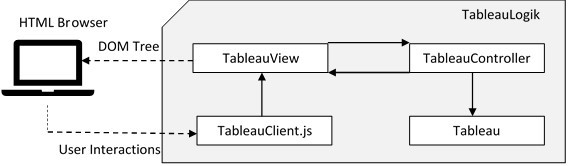
\includegraphics[width=1.0\textwidth]{Achitectur}
\caption[Achitektur]{Achitektur}\label{fig:Achitectur}
\end{figure}
Abbildung \ref{fig:Achitectur} zeigt die Architektur von der Tableau-Webanwendung im Überblick. Die Architektur folgt dem bewährten Model-View-Controller-Prinzip. Softwaretechnisch gliedert sich die
Anwendungslogik so in mehrere Komponenten (Klassen) mit spezifischen funktionalen Verantwortlichkeiten.
%Eine zentrale Rolle für die Anwendungssteuerung hat der Controller (Klasse TableauController). Der Controller kann Nutzerinteraktionen 
%erkennen und in entsprechende Modelinteraktionen umsetzen. Der Controller wird detailliert im Unterabschnitt \ref{subsec:Controller} erläutert.
Die \textit{``TableauClient.js''}
%, die im Unterabschnitt blablabla erläutert
 kann Nutzerinteraktionen erkennen und über den View an den Controller weiterleiten. Der Controller unter entsprechenden Nutzerinteraktionen in 
%Modelinteraktionen 
Model
umsetzen. Der Controller wird detailliert im Unterabschnitt \ref{subsec:Controller} erläutert.

Die \textit{TableauView} kapselt den DOM-Tree und bietet entsprechende Manipulationsmethoden für den Controller an, um sich verändernde Anwendungszustände im Browser zur Anzeige zu bringen. Der View wird im Unterabschnitt \ref{subsec:View} erläutert.

Konzeptionell wird die Tableau-Webanwendung in einem Model abgebildet. Das Model ist komplexer und gliedert sich in mehrere logische Entities, die sich aus den Grundlagen des Kapitels \ref{sec:Grundlagen} ableiten und im Unterabschnitt \ref{sec:Model} erläutert werden.

\section{Klassendiagramm}
Um einen genaueren Überblick zu erhalten, welche Klassen wie mit einander kommunizieren, eignet sich ein Klassendiagramm. Nachfolgend ist zu erkennen, in welcher Kommunikation die Klassen zueinander stehen.
\begin{figure}[ !h] \centering
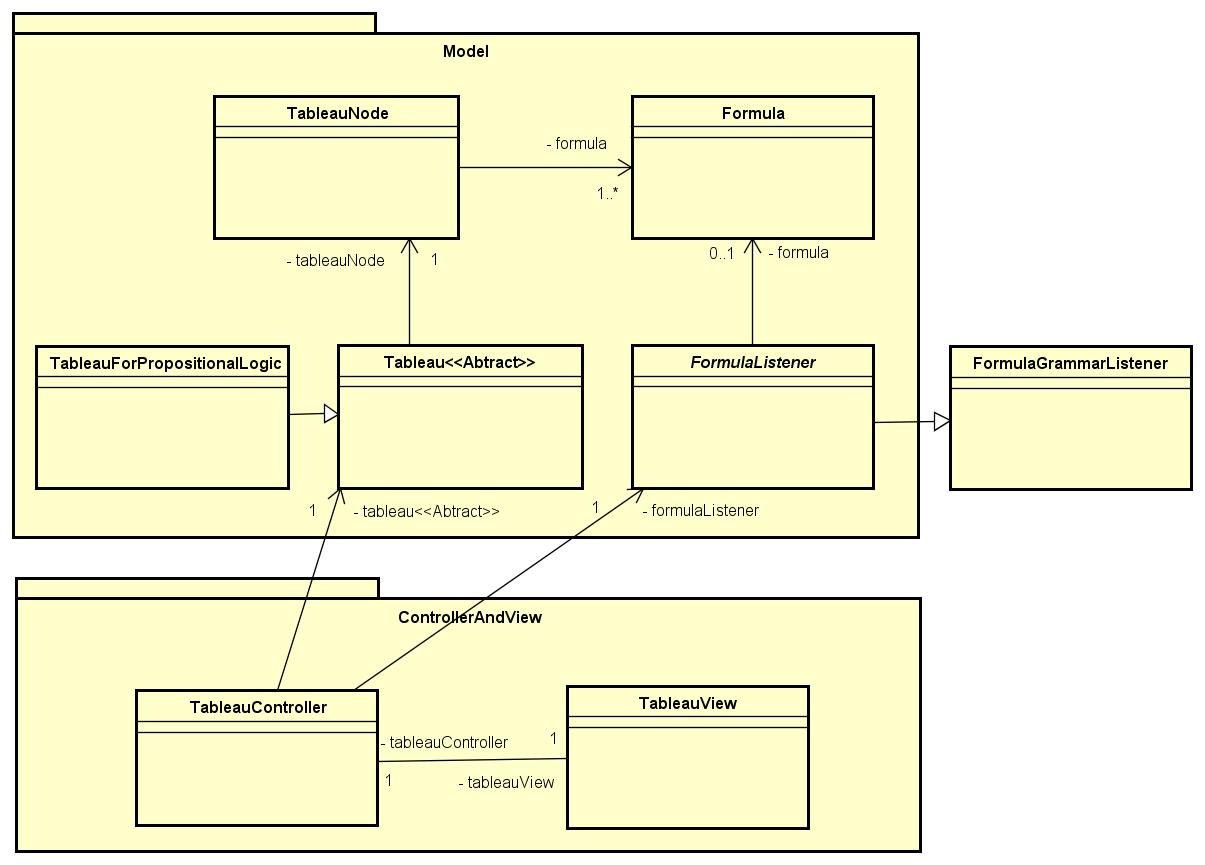
\includegraphics[width=1.0\textwidth]{ClassDiagram}
\caption[Klassendiagramm]{Klassendiagramm}\label{fig:Klassendiagramm}
\end{figure}

Tableau-Webanwendung umfasst verschiedene Bereiche:
\begin{itemize}
\item	Analyse der Eingabeformel und Darstellung einer Formel als Baumstruktur(\hyperlink{/LF10/}{/LF10/}): Klassen \textit{FormulaListener} und \textit{Formula}.
\item	Erstellung und Darstellung des Tableaus (\hyperlink{/LF20/}{/LF20/} und \hyperlink{/LF30/}{/LF30/}):  Klassen \textit{TableauNode}, \textit{Tableau} und \textit{TableauForPropositionalLogic}.
\item	Verarbeitung der GUI-Interaktionen (\hyperlink{/LF10/}{/LF10/}, \hyperlink{/LF20/}{/LF20/}, \hyperlink{/LF30/}{/LF30/} und \hyperlink{/LF40/}{/LF40/}): Klassen \textit{TableauView} und \textit{TableauController}.
\end{itemize}

Um die Möglichkeit zur Erweiterung der Software, gibt es eine abtrakte Klasse \textit{Tableau}, welche die Tableaus erweitern. Die abstrakte Klasse definiert die Basismethoden um ein Tableau zu erstellen. 


%\chapter{Implementierung}\label{sec:Implementierung}
In diesem Kapitel geht es um die Implementierung der Webanwendung. 

Wie im Abschnitt \ref {sec:Antlr4} erwähnt, kann man das Skript \textit {require.js} verwenden um das Importieren von dutzenden Dateien manuell zu vermeiden, wie im folgenden Beispiel gezeigt:

\begin{lstlisting}[language=HTML,basicstyle=\scriptsize]
    <script src="src/Enums.js"></script>
    <script src="src/Model/Formula.js"></script>
    <script src="src/Model/TableauNode.js"></script>   
    <script src="src/Model/TableauForPropositionalLogic.js"></script>
    ...
</body>
</html>
\end{lstlisting}
Diese Dateien müssen in der folgenden Reihenfolge geladen werden:
\begin{itemize}
\item	\textit{Enums.js} muss zuerst geladen werden, da alle anderen Dateien es benötigen.
\item	\textit{Formula.js} wird von \textit{TableauNode.js} verwendet und muss daher zuerst geladen werden.
\item	In ähnlicher Weise wird \textit{TableauNode.js} von \textit{TableauForPropositionalLogic.js} verwendet und muss daher als nächstes geladen werden.
\end{itemize}
Man kann leicht erkennen, dass das Laden von Dateien in der richtigen Reihenfolge wichtig ist, da sie voneinander abhängig sind. Dies mag zunächst kein Problem sein, aber wenn der Code kompliziert wird, wachsen die Dateien und es wird immer schwieriger, die \textit{script}-Tags zu verwalten.

%Wenn man die JavaScript Dateien manuell wie oben importiert, gibt es viele Nachteile wie \footnote{\url{https://frederic-hemberger.de/talks/requirejs/\# /3}}:
%\begin{itemize}
%\item	Websites werden immer komplexer.
%\item	Komplexer Code ist schlechter zu warten.
%\item	Komplexer Code ist schlechter zu testen.
%\item	Verwaltung der Abhängigkeiten von Hand ist fehleranfällig
%\end{itemize}

Daher wird \textit{require.js} im Rahmen dieser Arbeit nicht nur für die ANTLR-Bibliothek sondern für alle andere JavaScript-Dateien verwendet. \textit{require.js} implementiert die Funktion \textit{require()} von \textit{Node.js} im Browser. \textit{require()} wird zum Laden von Dateien verwendet. Für normale JavaScript-Dateien bedeutet dies, dass sie ausgeführt werden, wenn sie zum ersten Mal geladen werden, und das war es. Der Code wird in seiner eigenen Schließung ausgeführt, so dass er den Rest des Codes nicht stört (z.B. identische Variablennamen sind kein Problem). Die einzige Möglichkeit, etwas an die Außenwelt zurückzugeben, besteht darin, ein spezielles Objekt \textit{exports}, das aufgerufen wird, zu ändern , wobei dies der Rückgabewert des\textit{ require()} Aufrufs ist. Eine JavaScript-Datei, die \textit{exports} eine Funktion oder Variable an die Außenwelt zurückgibt, wird als ``Modul'' bezeichnet \cite{pixels}. Man kann \textit{require()} in seinem Browser wie folgt verwenden:

\begin{lstlisting}[language=HTML,basicstyle=\scriptsize]
<html>
<head>
	<script type="text/javascript" src="lib/require.js"></script>
</head>
<body>
	<script type="text/javascript">
		var Formula = require("src/Model/Formula.js").Formula;
		var formula =  new Formula("1", null, null, FormulaTypeEnum.TRUE);
		var type = formula.getFormulaType();
	</script>
</body>
</html>
\end{lstlisting}
Der Code in \textit{Formula.js} könnte so aussehen:
\begin{lstlisting}[language=JavaScript,basicstyle=\scriptsize]
function Formula(label, left, right, formulaType) {
    this.right = right;
    this.left = left;
    this.label = label;
    this.formulaType = formulaType;
}
Formula.prototype.getFormulaType = function () {
    return this.formulaType;
};

exports.Formula = Formula;
\end{lstlisting}

Die einzige Datei, die man normalerweise laden muss, ist \textit{require.js}, die definiert \textit{window.require()}. Danach kann man das Modul \textit{Formula.js} wie in \textit{Node.js} laden. Die Variable \textit{Formula} enthält alle vom Modul exportierten Daten, so dass man sich diese als ``Namespace'' vorstellen kann. Das Aufrufen einer exportierten Funktion \textit{getFormulaType()} in diesem Fall, funktioniert genauso wie das Aufrufen der Methode eines Objekts. Von hier werden alle exportierten Funktionen als ``Methoden'' bezeichnet.

Im Rahmen dieser Arbeit werden alle sogenannten ``Namespaces'' im Skript \textit{Global.js} definiert. Weiterhin enthält das Skript auch alle globalen Variablen der Anwendung.

\begin{itemize}
\item \textit{view}: globale Instanz der Klasse \textit{TableauView}
\item \textit{InputError}: Boolean Variable, ist ``true'' wenn es eine Antlr-Fehlermeldung gibt.
\item \textit{ErrorMessage}: Ein Array um die Antlr-Fehlermeldungen zu speichern.
\item \textit{TableauChartData}: ``Google Charts DataTable'' um das Tableau zu visualisieren.
\item \textit{ArrOfTableauNodesByStepByStep}: Ein Array speichert die Tableau-Knoten für den Tableau-Chart in einem Schritt der ``Schritt für Schritt Lösung'' (wird in der Methode drawTableauChartStepByStep() verwendet).
\item \textit{ArrOfAllTableauNodes}: Ein Array speichert die übrige Tableau-Knoten, die noch nicht für den Tableau-Chart der ``Schritt für Schritt Lösung'' benutzt werden (wird in der Methode drawTableauChartStepByStep() verwendet). 
\item \textit{TableauStepByStepData}: ``Google Charts DataTable'' um das Tableau für die ``Schritt für Schritt Lösung'' zu visualisieren.
\item \textit{stepNr}: Ordnungszahl des aktuellen Schrittes (wird für ``Schritt für Schritt Lösung'' verwendet).
\item \textit{chartNr}: Ordnungszahl des aktuellen Organigramm (wird für ``Schritt für Schritt Lösung'' verwendet).
\item \textit{nexStepNr}: Ordnungszahl des nächsten Schrittes (wird für ``Schritt für Schritt Lösung'' verwendet).
\item \textit{isTautology}:  Ergebnis der Tautologie-Prüfung. Die Variable wird in der Enumeration \textit{TautologyOrSatisfiableEnum} definiert (default: \textit{TautologyOrSatisfiableEnum.NOTTESTED}, wenn die Tautologie nicht geprüft wird).
\item \textit{isSatifiable}:   Ergebnis der	Erfüllbarkeit-Prüfung. Die Variable wird in der Enumeration \textit{TautologyOrSatisfiableEnum} definiert (default: \textit{TautologyOrSatisfiableEnum.NOTTESTED}, wenn die Erfüllbarkeit nicht geprüft wird).
\begin{lstlisting}[language=JavaScript, caption= TautologyOrSatisfiableEnum,basicstyle=\scriptsize]
const TautologyOrSatisfiableEnum = Object.freeze({
    TRUE: "TRUE",
    FALSE: "FALSE",
    NOTTESTED: "NOTTESTED"
});
exports.TautologyOrSatisfiableEnum = TautologyOrSatisfiableEnum;
\end{lstlisting}
\end{itemize}
%\chapter{Softwaretest}\label{sec:Softwaretest}
Der Softwaretest umfasst eine Nachweisstrategie und die Vorgaben der Entwicklung, um eine hochwertige Anwendung zu erstellen.

Die Nachweisstrategie beschreibt die Anwendung von Unit-Test auf das Gesamtsystem, insbesondere die Festlegung des Einsatzes und das Code Coverage.

Vorgaben für die Entwicklungsumgebung umfasst die Konfiguration der Unit-Tests/ Code Coverage Tools und die Verwendung der Testergebnisse.

\section{Konzept zum Softwaretest}
Das Konzept umfasst das Testverfahren während der Entwicklung mit abschließender Testdokumentation.

Folgende Anforderungen stellt das Konzept an das Testverfahren
\begin{itemize}
\item	Jede Methode wird mit Unit-Tests getestet. 
\item	Die Unit-Tests werden begleitend zur Entwicklungsphase geschrieben und erweitert
\item	Abschließend decken die Unit-Tests mindestens 85\% der implementierten Methoden ab, Frameworks ausgenommen
\item 	Regelmäßiges Prüfen der Code Coverage
\end{itemize}

Während des Entwicklungsprozesses wurden die Unit-Test kontinuierlich vervollständigt und mittels Code Coverage geprüft, ob die Testabdeckung ausreichend ist.

Die Unit-Tests wurden mit Hilfe von Jasmine erstellt.  Mittels zwei HTML-Dateien  \textit{``UnitTestModel.html''} und \textit{``UnitTestControllerView.html''} werden die Tests integriert. Darin erhält \textit{``UnitTestModel.html''} die Tests für das Model. Und \textit{``UnitTestControllerView.html''} enthält die Tests für den Controller und die View sowie einer Kopie der \textit{indexTableau.html} Dateien um die Manipulation des DOM-Tree zu testen. In der Datei \textit{``UnitTestModel.html''} wird das Test-Framework Jasmine im head-Tag eingebunden (Listing \ref{lis:EinbildungModel}). Dagegen wird Jasmine in der Datei \textit{``UnitTestControllerView.html''} am Ende der Seite im  body-Tag eingebunden, da es notwendig ist, dass das Markup vollständig geladen ist, bevor mit den Test begonnen werden kann (Listing \ref{lis:EinbildungControllerView}).
\begin{lstlisting}[language=HTML, caption= Einbildung Jasmine und Test-Dateien (Model), label=lis:EinbildungModel,basicstyle=\scriptsize]
<script src="lib/jasmine-3.1.0/jasmine.js"></script>
[...]
    <script src="lib/jasmine-3.1.0/jasmine-html.js"></script>
    <script src="lib/jasmine-3.1.0/boot.js"></script>

    <!--incl. Test files here...-->
    <script src="Tests/FormulaListenerUnitTest.js"></script>
    <script src="Tests/FormulaUnitTest.js"></script>
    <script src="Tests/TableauNodeUnitTest.js"></script>
    <script src="Tests/TableauForPropositionalLogicUnitTest.js"></script>
</head>
<body>
</body>
</html>
\end{lstlisting}

\begin{lstlisting} [language=HTML, caption= Einbildung Jasmine und Test-Dateien (Controller und View),label=lis:EinbildungControllerView, basicstyle=\scriptsize]
[...]
<!--incl. Test files here...-->
<script src="src/Global.js"></script>
<script src="src/TableauClient.js"></script>
<script src="Tests/TableauControllerAndViewUnitTest.js"></script>
</body>
\end{lstlisting}

Der Aufbau von Tests sieht wie folgt aus (Listing \ref{lis:FormulaTest}):

\begin{lstlisting} [language=JavaScript, caption= Beispiel Test der Klasse Formula, label=lis:FormulaTest, basicstyle=\scriptsize]
describe("Unit Tests for Formula", function() {
    var left = new Formula("p", null, null,FormulaTypEnum.POSITIVLITERAL);
    var right = new Formula("p", null ,null,FormulaTypEnum.POSITIVLITERAL);
    var root = new Formula(FormulaOperatorEnum.AND,left,right, FormulaTypEnum.ALPHA);
    var negation =  new Formula(FormulaOperatorEnum.NEG,null,root, FormulaTypEnum.BETA);

    it("p&q has type as ALPHA, p and p have types as POSITIVLITERAL", function() {
        expect(left.getFormulaTyp()).toEqual(FormulaTypEnum.POSITIVLITERAL);
        expect(right.getFormulaTyp()).toEqual(FormulaTypEnum.POSITIVLITERAL);
        expect(root.getFormulaTyp()).toEqual(FormulaTypEnum.ALPHA);

    });
    it("p&q has left child as p and right child as p", function() {
        expect(root.getLeft()).toEqual(left);
        expect(root.getRight()).toEqual(right);
    });

    it("p has negative formula as !p", function() {
        expect(left.getNegativeFormula()).toEqual(new Formula(FormulaOperatorEnum.NEG,null,p,FormulaTypEnum.NEGATIVLITERAL));
    });
	[...]
});
\end{lstlisting}


\section{Evaluation der Testfälle}
Es gibt insgesamt 72 Unit-Tests für das Model (Abbildung \ref{fig:TestResultModel}) und 16 Unit-Tests für den Controller und die View (Abbildung \ref{fig:TestResultControllerView}).

\begin{figure}[ !h] \centering
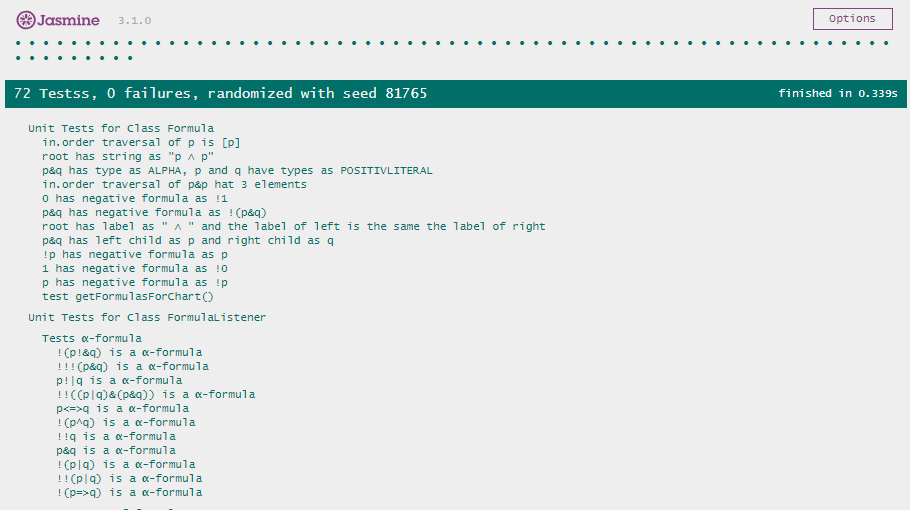
\includegraphics[width=1.0\textwidth]{TestResultModel}
\caption[Testergebnisse des Models]{Ein Teil der Testergebnisse des Models}\label{fig:TestResultModel}
\end{figure}

\begin{figure}[ !h] \centering
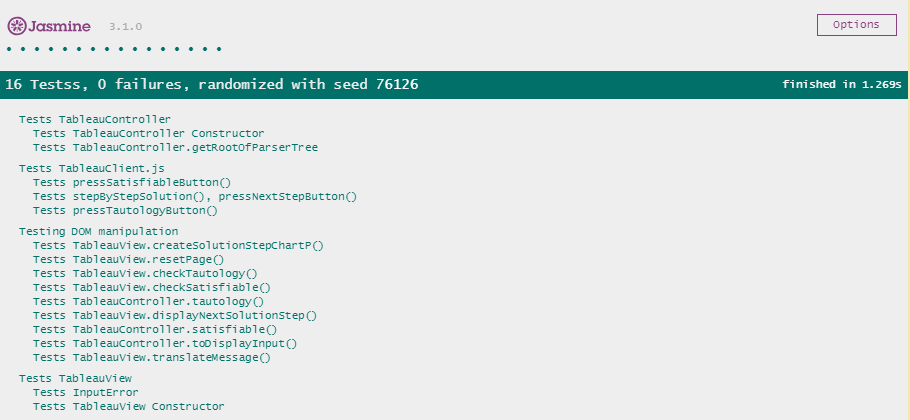
\includegraphics[width=1.0\textwidth]{TestResultControllerView}
\caption[Testergebnisse des Controllers und der View]{Testergebnisse des Controllers und der View}\label{fig:TestResultControllerView}
\end{figure}

Die Tests sind nach der Klasse gruppiert und können dementsprechend zielgerichtet evaluiert werden.
\begin{itemize}

\item \textit{FormulaUnitTest.js}: Enthält 12 Tests für die Klasse \textit{Formula}, wobei alle Methoden der Klasse \textit{Formula} mindestens einmal überprüft werden. Die Methode \textit{getNegativeFormula()} wird mit den Eingabeformeln als Konstante True/False, positive-/negative-Literal, $\alpha $- und  $\beta $-Formel überprüft.

\item \textit{FormulaListenerUnitTest.js}: Enthält 30 Tests. Diese Tests untersuchen die Struktur einer Formel wie linken (\textit{left}) und rechten (\textit{right}) Teilbaum, inhalt (\textit{label}) und Formeltypen (\textit{formulaType}) nachdem sie mithilfe der Klasse \textit{FormulaListener} von Zeichenkette in einen Baum konvertiert wurden. Für jeden Formeltyp (Konstante True/False, positive-/negative-Literal, $ \alpha $- und  $ \beta $-Formel) und für jede Regel der Klassifizierung von $\alpha$- und $\beta$-Formeln wird mindestens eine Formel überprüft.

\item \textit{TableauNodeUnitTest.js}: Enthält 12 Tests für die Klasse \textit{TableauNode}, wobei alle Methoden der Klasse \textit{TableauNode} mindestens einmal überprüft werden. Alle Methoden, die den booleschen Wert zurückgeben, werden mindestens zweimal mit den Rückgabewerten false und true überprüft. Die Methoden \textit{containsOnlyLiterals()}, \textit{containsAComplementaryPairOfLiterals()} und \textit{containsAlphaFormula()} werden mit den Tableau-Knoten, die mit der Menge von Formeln $\{q\}$, $\{p\wedge(q\vee\neg p)\}$, $\{p,q\}$, $\{p,\neg p\}$, $\{\neg p,p\}$, $ \{p,q\vee\neg p\} $, $\{p,\neg p,\neg\neg p\}$, $\{p,1\}$ und $\{q,0\}$ markiert sind, getestet.

\item \textit{TableauForPropositionalLogicUnitTest.js}: Enthält 18 Tests für die Klasse \textit{TableauForPropositionalLogic}, wobei alle Methoden der Klasse \textit{TableauForPropositionalLogic} mindestens einmal überprüft werden. Die Methoden \textit {determineAlphaFormulas()} und \textit{determineBetaFormulas()} werden für jede Regel der Klassifizierung von $\alpha$- und $\beta$-Formeln mindestens einmal überprüft.

\item \textit{TableauControllerandViewUnitTest.js}: Enthält 16 Tests für die Klassen \textit{TableauView}, \textit{TableauController}, \textit{TableauClient.js} und \textit{TableauClient.js} wobei alle Methoden mindestens einmal überprüft werden. Die Methoden \textit { pressSatisfiableButton()} und \textit{pressTautologyButton()} werden für eine syntaktisch korrekte Formel und eine fehlerhafte Formel einmal überprüft.
\end{itemize}


\section{Code Coverage}

\begin{figure}[ !h] \centering
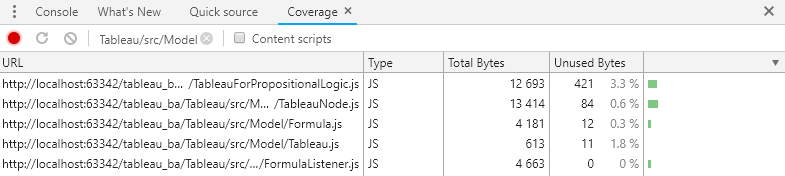
\includegraphics[width=1.0\textwidth]{TestCoverageModel2}
\caption[Code Coverages des Models]{Code Coverages des Models}\label{fig:TestCoverageModel}
\end{figure}

\begin{figure}[ !h] \centering
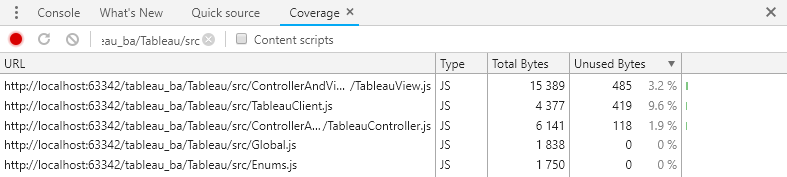
\includegraphics[width=1.0\textwidth]{TestCoverageControllerView5}
\caption[Code Coverages des Controllers und der View]{Code Coverages des Controllers und der View}\label{fig:TestCoverageClientLogik}
\end{figure}

Um eine Code Coverage zu messen, ist ein weiteres Tool notwendig. Es gibt dafür Chrome DevTools, das besteht aus einer Reihe von Webentwicklungs-Tools, die direkt in den Google Chrome-Browser integriert sind. Die neueste DevTools Version (Chrome 59) bietet eine neue Registerkarte ``Coverage'' an. Wenn man eine Seite lädt oder ausführt, erfährt man auf dieser Registerkarte, wie viel Prozent des heruntergeladenen Codes, noch nicht verwendet wurde \cite{Kayce}.
Die Ergebnisse der Codeabdeckung sind unter den Abbildungen \ref{fig:TestCoverageModel} und \ref{fig:TestCoverageClientLogik} zu sehen.

Alle Dateien erfüllen die Mindestgrenze unter Rücksichtnahme, dass das Tool bei \textit{switch-case} und \textit{if-clause}(ohne \textit{else}) nicht richtig ausgewertet werden konnte. Außerdem konnte das Tool auch nicht jedes Event des GUI mit auswerten, deshalb kommt es zu verfälschten Ergebnissen (Abbildung \ref{fig:FehlerCoverage}).

\begin{figure}[ !h] \centering
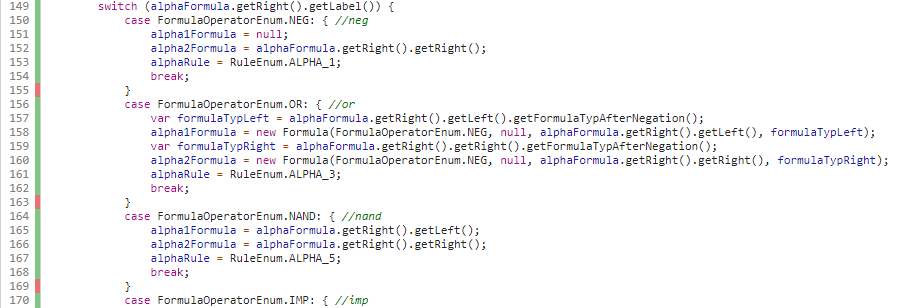
\includegraphics[width=1.0\textwidth]{FehlerCoverage}
\caption[Problem bei CodeCoverages]{Problem bei Code Coverages}
\label{fig:FehlerCoverage}
\end{figure}
%\chapter{Zusammenfassung}
Diese Arbeit hat die beschriebenen Anforderungen erfüllt. Die Kernaufgabe besteht darin, eine Webanwendung für ein semantisches Tableau zu entwickeln, um ermitteln zu können, ob eine Formel erfüllbar oder allgemeingültig ist. Darüber hinaus kann die Anwendung die Struktur von einem Tableau über Google Chart Tools visualisieren. Zur Unterstützung bei dem Erlernen der Konstruktion eines semantischen Tableaus bietet die Anwendung auch eine ``Schritt für Schritt Lösung'' -Funktion, wonach Studierende Schritt für Schritt den Aufbau eines Tableaus folgen können. Nicht nur das, die Anwendung wurde entwickelt, um eine Vielzahl von Geräten von Desktop bis Smartphone zu unterstützen.

Es wäre ideal, wenn die Anwendung in Zukunft weiterentwickelt  werden könnte, zum Beispiel: Unterstützung für die prädikatenlogischen Formeln oder Verwendung eines Offline-Frameworks, um ein Tableau ohne Internetverbindung visualisieren zu können.


%
%\include{Literatur}
%
%\bibliographystyle{plain}
%\thispagestyle{empty}
%\bibliography{bib}
%\end{document}

% ---------------------------------------------------------------
\frontmatter % Titelblätter und Erklärung
    \pagestyle{empty} % Seitennummerierung abschalten
		%%%%%%%%%%%%%%%%%%%%%%%%%%%%%%%
% Seite als zus�tzliches Deckblatt, optional

%\thispagestyle{empty}

%\begin{center}

%\vspace*{-2cm}

%
\includegraphics[width=1.2\textwidth]{fhl_logo}

%\vspace*{5cm}

%{\Large \textbf{Bachelorarbeit}}\\ % oder Masterarbeit, Projektbericht, etc.

%\vspace{4.0cm}
%{\Huge \textbf{Anleitung zum Erstellen}}\\
%\vspace*{3mm}
%{\Huge \textbf{einer Abschlussarbeit}}\\
%\vspace*{3mm}
%{\Huge \textbf{}}\\
%\vspace{1.5cm}

%{\LARGE Andreas Hanemann} % Name des Autors

%\vspace{3cm}
%Entwurf vom \today % erleichtert den Betreuern die Zuordnung - f�r finale Version entfernen

%\end{center}

%\newpage

%%%%%%%%%%%%%%%%%%%%%%%%%%%%%%%
% zweite Seite

%\thispagestyle{empty}
%\cleardoublepage

%%%%%%%%%%%%%%%%%%%%%%%%%%%%%%%
% dritte Seite (im wesentlichen Kopie der ersten)

\thispagestyle{empty}

\begin{center}

\vspace*{-2cm}


\includegraphics[width=1.2\textwidth]{fhl_logo}

\vspace*{3cm}

{\Large \textbf{Bachelorarbeit}}\\ % oder Masterarbeit, Projektbericht, etc.

\vspace{2.0cm}
{\Huge \textbf{Webanwendung zur Unterstützung }}\\
\vspace*{3mm}
{\Huge \textbf{des Lernens der Methode}}\\
\vspace*{3mm}
{\Huge \textbf{Semantisches Tableau}}\\
\vspace*{3mm}
{\Huge \textbf{}}\\
\vspace*{3mm}
{\Huge \textbf{}}\\

\vspace{1.5cm}

%vorgelegt von
%\vspace{1.5cm}
%
%{\LARGE Tram Nguyen} % Name des Autors
\vspace{4cm}

\parbox{1cm}{
\begin{large}
\begin{tabbing}
%Ausgabedatum: \hspace{.5cm} \=04. Juni 2018\\
%Abgabedatum: \>04. September 2018\\
vorgelegt von: \hspace{.5cm} \=Tram Nguyen\\

Erstbetreuer: \>Prof. Dr. rer. nat. Andreas Schäfer\\
Zweitbetreuer: \>Prof. Dr.-Ing. Stefan Krause\\
\end{tabbing}
\end{large}}\\
\vspace{5mm}
%(Prof.~ Dr.~ rer.~ nat. Andreas Hanemann)\\
%Vorsitzender des Pr�fungsausschusses
\end{center}
 % Titelblätter FHL 
    \cleardoublepage
   % \include{abstract} % Abstract 
    %\cleardoublepage
    \include{erklaerung-fhl} % Erklärung (Arbeit selbstständig verfasst)
		\cleardoublepage
    %\include{danksagung} % optional
    \tableofcontents % Inhaltsverzeichnis
    \addtocontents{toc}{\protect\thispagestyle{empty}}
		
% ---------------------------------------------------------------
\mainmatter % die eigentliche Arbeit
    \pagestyle{headings}
 \font\riesigeKapNummer = cmssdc10 at 72.72pt %% scaled \magstep5

\newcommand{\Datum}{\today}
\pagestyle{fancy}
\addtolength{\headwidth}{\marginparsep}
%\addtolength{\headwidth}{\marginparwidth}
\addtolength{\headheight}{2pt}
%%
%\renewcommand{\baselinestretch}{2.0}
\setlength{\parskip}{0.8em}
\renewcommand{\chaptermark}[1]{\markboth{\thechapter\ #1}{}}
\renewcommand{\sectionmark}[1]{\markright{\thesection\ #1}}
\renewcommand{\indexname}{Index}
\fancyhf{}
\fancyhead[LE,RO]{\sffamily\thepage}
\fancyhead[LO]{\sffamily\rightmark} \fancyhead[RE]{\sffamily\leftmark}
      \cfoot{}

\fancypagestyle{plain}{%
    \fancyhead{}
   % \fancyfoot[LO]{\sf\fs T. Nguyen: Bachelorarbeit (\Datum)}
    \fancyfoot[RO]{\sf\thepage}
    \renewcommand{\headrulewidth}{0pt} %keine Linie in der Fußzeile
    }
\allsectionsfont{\sffamily }
\chaptertitlefont{\Huge\sffamily\raggedleft }
\chapternumberfont{\riesigeKapNummer \raggedleft}

\newcommand{\fs}{\footnotesize }
\newcommand{\mc}[3]{\multicolumn{#1}{#2}{#3}}

\def\DraftMode{false}
%\def\DraftMode{true}

\title{Bachelorarbeit }
\author{Tram Nguyen}
\date{\today}

\chapter{Einleitung}
Aussagenlogik ist immer ein grundlegendes Thema in der Informatik. Dabei ist die Ermittlung der Allgemeingültigkeit oder Erfüllbarkeit einer aussagenlogischen Formel unverzichtbar. Es gibt viele Möglichkeiten, dies zu tun, wobei die Verwendung der Wahrheitstafel recht aufwändig sein kann. Die Äquivalenzumformung liefert auch kein Verfahren, das sagt, welche Regel anzuwenden ist \cite{Schaefer}.
%eine häufig verwendete Methode die Verwendung der Äquivalenzen ist. Diese Methode bietet jedoch keine Möglichkeit zu wissen, welche Regeln gelten, so dass der Verwender ein umfangreiches Training benötigt, um dies zu lösen.
Auch diese Methode ist schwer zu programmieren. Eine andere Methode ist einfacher und intuitiver:  Eine Formel der Aussagenlogik kann als ein semantisches Tableau nach syntaktischen Regeln konstruiert werden. Aus dem derart konstruierten Tableau kann dann ermittelt werden, ob eine Formel erfüllbar oder allgemeingültig ist. Diese Methode kann auch einfach programmiert werden. Dies sind jedoch neue Inhalte, die seit dem WS 2017-2018 in den Lehrplan der Informatik 1 aufgenommen wurden. Um den Studierenden den Erwerb dieser Methode zu erleichtern, wird daher die Idee einer Webanwendung gebildet.

Das Hauptziel dieser Arbeit ist es, eine Webanwendung zu entwickeln. Es ermöglicht dem Benutzer, eine aussagenlogische Formel einzugeben und die Allgemeingültigkeit oder Erfüllbarkeit der Formel zu überprüfen. Zuerst prüft die Anwendung, ob die Formel syntaktisch korrekt ist. Wenn dies nicht der Fall ist, wird die Anwendung den Benutzer informieren, um es zu beheben. Die Anwendung zeigt dann die Konstruktionen für die Eingabeformel und für das Tableau an. Schließlich wird das Prüfergebnis auf dem Bildschirm angezeigt.

Der Inhalt dieser Arbeit gliedert sich in 6 Hauptteile. Die erste besteht darin, das Problem und die Anforderungen der Anwendung zu analysieren (Kapitel \ref{sec:Analyse}). Als nächstes lernt man etwas über die Grundlagen der Aussagenlogik (Kapitel \ref{sec:Grundlagen}) und man wählt die geeigneten Frameworks (Kapitel \ref{sec:Frameworks}). Als nächstes soll die Architektur der Anwendung (Kapitel \ref{sec:Architektur}) erstellt und umgesetzt werden (Kapitel \ref{sec:Implementierung}). Abschließend: Anwendungstests und Test-Bewertung (Kapitel \ref{sec:Softwaretest})

\cleardoublepage

\cleardoublepage
%\chapter{Analyse} \label{sec:Analyse}
Dieses Kapitel handelt von der Problemanalyse sowie den Anforderungsdefinitionen der Anwendung.

\chapter{Analyse} \label{sec:Analyse}
Dieses Kapitel handelt von der Problemanalyse sowie den Anforderungsdefinitionen der Anwendung.

%	\section{Problemanalyse: Lastenheft}
\begin{enumerate}
\item \textbf{Zielbestimmung}
%Es gibt viele Möglichkeiten, wie zum Beispiel das Wahrheitstafelverfahren oder die Äquivalenzumformung, um zu prüfen, ob eine Formel der Aussagenlogik allgemeingültig ist. Die Wahrheitstabellen sind unpraktikabel, da sie exponentiell wachsen. Die Äquivalenzumformung liefert auch kein Verfahren, das sagt, welche Regel anzuwenden ist. Es gibt auch ein alternatives Verfahren, das die Erfüllbarkeit einer aussagenlogischen Formel überprüft. Ebenso gibt es das sogenannte Tableau-Verfahren. 
Es gibt ein Verfahren, das die Erfüllbarkeit einer aussagenlogischen Formel überprüft, die Tableau-Verfahren genannt wird.
Dazu werden systematische Regeln angewendet und Formeln umgeschrieben. Dieses Verfahren kann auch als Programm implementiert und genutzt werden. Daher soll, um das Lehren und Lernen der Informatikmodule besser zu unterstützen, eine Software entwickelt werden, die vom Nutzer eine aussagenlogische Formel annimmt und prüft, ob diese Formel erfüllbar oder allgemeingültig ist. Das Ergebnis soll mittels eines semantischen Tableaus erstellt und angezeigt werden. Außerdem soll die Anwendung eine ``Schritt für Schritt Lösung''- Funktion, wonach Studierende Schritt für Schritt den Aufbau eines Tableaus folgen können, bieten. Die Software soll als Web-Applikation eingeführt werden.

\item \textbf{Produkteinsatz}

\hypertarget{/LE10/}{/LE10/} Verwendung im Bereich Lehren und Lernen der Informatikmodule.

\hypertarget{/LE20/}{/LE20/} Die Nutzer sollen die Funktionalität über eine Webanwendung nutzen können.	

\hypertarget{/LE30/}{/LE30/} Die Software soll ohne Server und Datenbank funktionieren können.

\hypertarget{/LE40/}{/LE40/} Zielgruppe der Software sind Studierende und die Dozierende.

\item \textbf{Produktfunktionen}

\hypertarget{/LF10/}{/LF10/} Eingabeformel überprüfen und anzeigen
\begin{itemize} 
\item Die Software prüft, ob die Eingabeformel ein wohlgeformter Ausdruck der Aussagenlogik ist, sonst Wiederholung der Eingabe.
\item Die Eingabeformel-Darstellung wird als Baumstruktur erstellt und in dem GUI angezeigt .
\end{itemize}


\hypertarget{/LF20/}{/LF20/} Allgemeingültigkeit überprüfen und Tableau darstellen
\begin{itemize}
\item Die Software erstellt die Negation von der Eingabeformel. 
\item Die Software  mittels Tableau-Verfahren prüft, ob diese Negation erfüllbar ist (/LF30/).
\item Wenn diese Negation nicht erfüllbar ist, ist die Eingabeformel allgemeingültig.
\item Wenn diese Negation erfüllbar ist, ist die Eingabeformel nicht allgemeingültig.
\item Die Tableau-Darstellung wird als Baumstruktur erstellt und in dem GUI angezeigt.
\end{itemize}

\hypertarget{/LF30/}{/LF30/}  Erfüllbarkeit überprüfen und Tableau darstellen
\begin{itemize} 
\item Die Software mittels Tableau-Verfahren prüft, ob Eingabeformel erfüllbar ist
\item Die Tableau-Darstellung wird als Baumstruktur erstellt und in dem GUI angezeigt.
\end{itemize}


\hypertarget{/LF40/}{/LF40/}  Schritt für Schritt Lösung anzeigen
\begin{itemize}
\item Ein Pop-up Fenster von der Schritt für Schritt Lösung wird geöffnet.
\item Durch Anklicken eines Buttons kann das Tableau Stück für Stück dargestellt werden und ein Lösungshinweis für jeden Schritt angezeigt werden.
\end{itemize}

\item \textbf{Produktdaten}
\begin{itemize}
\item keine Produktdaten
\end{itemize}

\item \textbf{Produktleistungen}

/LL10/ Die Funktionen /LF20/ und /LF30/ darf nicht länger als 5 Sekunden Reaktionszeit benötigen

/LL20/ Bei fehlerhaften Eingaben erhält der Nutzer eine Fehlermeldung

/LL30/ Bei fehlerhaften Eingaben muss der Nutzer die Möglichkeit haben, eine Korrektur der Eingaben vorzunehmen.

                                                                                                                                                                                                                                                    
\item \textbf{Qualitätsanforderungen}

\hypertarget{/LQ10/}{/LQ10/} Vollständigkeit: Alle implementierten Funktionen werden benutzt. Alle referenzierten Funktionen werden implementiert.

\item \textbf{Ergänzungen}
\begin{itemize}
\item  Die Software soll zunächst unter \hypertarget{Chrome}{Chrome} laufen, langfristig aber auch unter Firefox und weiteren Browsern. 
\end{itemize}

%\item \textbf{Glossar}
%\begin{itemize}
%\item Reaktionszeit:  Zeitdauer bis eine Funktion ausgeführt ist.
%\end{itemize}
\end{enumerate} 


	\section{Problemanalyse: Lastenheft}
\begin{enumerate}
\item \textbf{Zielbestimmung}
%Es gibt viele Möglichkeiten, wie zum Beispiel das Wahrheitstafelverfahren oder die Äquivalenzumformung, um zu prüfen, ob eine Formel der Aussagenlogik allgemeingültig ist. Die Wahrheitstabellen sind unpraktikabel, da sie exponentiell wachsen. Die Äquivalenzumformung liefert auch kein Verfahren, das sagt, welche Regel anzuwenden ist. Es gibt auch ein alternatives Verfahren, das die Erfüllbarkeit einer aussagenlogischen Formel überprüft. Ebenso gibt es das sogenannte Tableau-Verfahren. 
Es gibt ein Verfahren, das die Erfüllbarkeit einer aussagenlogischen Formel überprüft, die Tableau-Verfahren genannt wird.
Dazu werden systematische Regeln angewendet und Formeln umgeschrieben. Dieses Verfahren kann auch als Programm implementiert und genutzt werden. Daher soll, um das Lehren und Lernen der Informatikmodule besser zu unterstützen, eine Software entwickelt werden, die vom Nutzer eine aussagenlogische Formel annimmt und prüft, ob diese Formel erfüllbar oder allgemeingültig ist. Das Ergebnis soll mittels eines semantischen Tableaus erstellt und angezeigt werden. Außerdem soll die Anwendung eine ``Schritt für Schritt Lösung''- Funktion, wonach Studierende Schritt für Schritt den Aufbau eines Tableaus folgen können, bieten. Die Software soll als Web-Applikation eingeführt werden.

\item \textbf{Produkteinsatz}

\hypertarget{/LE10/}{/LE10/} Verwendung im Bereich Lehren und Lernen der Informatikmodule.

\hypertarget{/LE20/}{/LE20/} Die Nutzer sollen die Funktionalität über eine Webanwendung nutzen können.	

\hypertarget{/LE30/}{/LE30/} Die Software soll ohne Server und Datenbank funktionieren können.

\hypertarget{/LE40/}{/LE40/} Zielgruppe der Software sind Studierende und die Dozierende.

\item \textbf{Produktfunktionen}

\hypertarget{/LF10/}{/LF10/} Eingabeformel überprüfen und anzeigen
\begin{itemize} 
\item Die Software prüft, ob die Eingabeformel ein wohlgeformter Ausdruck der Aussagenlogik ist, sonst Wiederholung der Eingabe.
\item Die Eingabeformel-Darstellung wird als Baumstruktur erstellt und in dem GUI angezeigt .
\end{itemize}


\hypertarget{/LF20/}{/LF20/} Allgemeingültigkeit überprüfen und Tableau darstellen
\begin{itemize}
\item Die Software erstellt die Negation von der Eingabeformel. 
\item Die Software  mittels Tableau-Verfahren prüft, ob diese Negation erfüllbar ist (/LF30/).
\item Wenn diese Negation nicht erfüllbar ist, ist die Eingabeformel allgemeingültig.
\item Wenn diese Negation erfüllbar ist, ist die Eingabeformel nicht allgemeingültig.
\item Die Tableau-Darstellung wird als Baumstruktur erstellt und in dem GUI angezeigt.
\end{itemize}

\hypertarget{/LF30/}{/LF30/}  Erfüllbarkeit überprüfen und Tableau darstellen
\begin{itemize} 
\item Die Software mittels Tableau-Verfahren prüft, ob Eingabeformel erfüllbar ist
\item Die Tableau-Darstellung wird als Baumstruktur erstellt und in dem GUI angezeigt.
\end{itemize}


\hypertarget{/LF40/}{/LF40/}  Schritt für Schritt Lösung anzeigen
\begin{itemize}
\item Ein Pop-up Fenster von der Schritt für Schritt Lösung wird geöffnet.
\item Durch Anklicken eines Buttons kann das Tableau Stück für Stück dargestellt werden und ein Lösungshinweis für jeden Schritt angezeigt werden.
\end{itemize}

\item \textbf{Produktdaten}
\begin{itemize}
\item keine Produktdaten
\end{itemize}

\item \textbf{Produktleistungen}

/LL10/ Die Funktionen /LF20/ und /LF30/ darf nicht länger als 5 Sekunden Reaktionszeit benötigen

/LL20/ Bei fehlerhaften Eingaben erhält der Nutzer eine Fehlermeldung

/LL30/ Bei fehlerhaften Eingaben muss der Nutzer die Möglichkeit haben, eine Korrektur der Eingaben vorzunehmen.

                                                                                                                                                                                                                                                    
\item \textbf{Qualitätsanforderungen}

\hypertarget{/LQ10/}{/LQ10/} Vollständigkeit: Alle implementierten Funktionen werden benutzt. Alle referenzierten Funktionen werden implementiert.

\item \textbf{Ergänzungen}
\begin{itemize}
\item  Die Software soll zunächst unter \hypertarget{Chrome}{Chrome} laufen, langfristig aber auch unter Firefox und weiteren Browsern. 
\end{itemize}

%\item \textbf{Glossar}
%\begin{itemize}
%\item Reaktionszeit:  Zeitdauer bis eine Funktion ausgeführt ist.
%\end{itemize}
\end{enumerate} 


	\section{Anforderungsanalyse}
\subsection{Anwendungsfalldiagramm}
\begin{figure}[ !h] \centering
%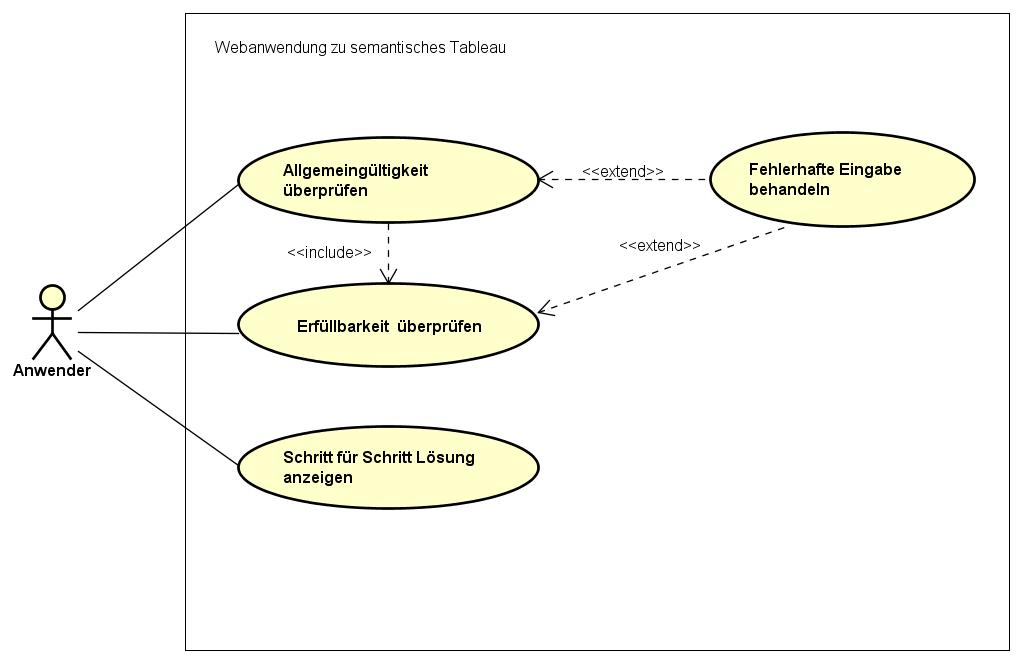
\includegraphics[width=1.0\textwidth,draft=\DraftMode]{UsecaseDiagram}
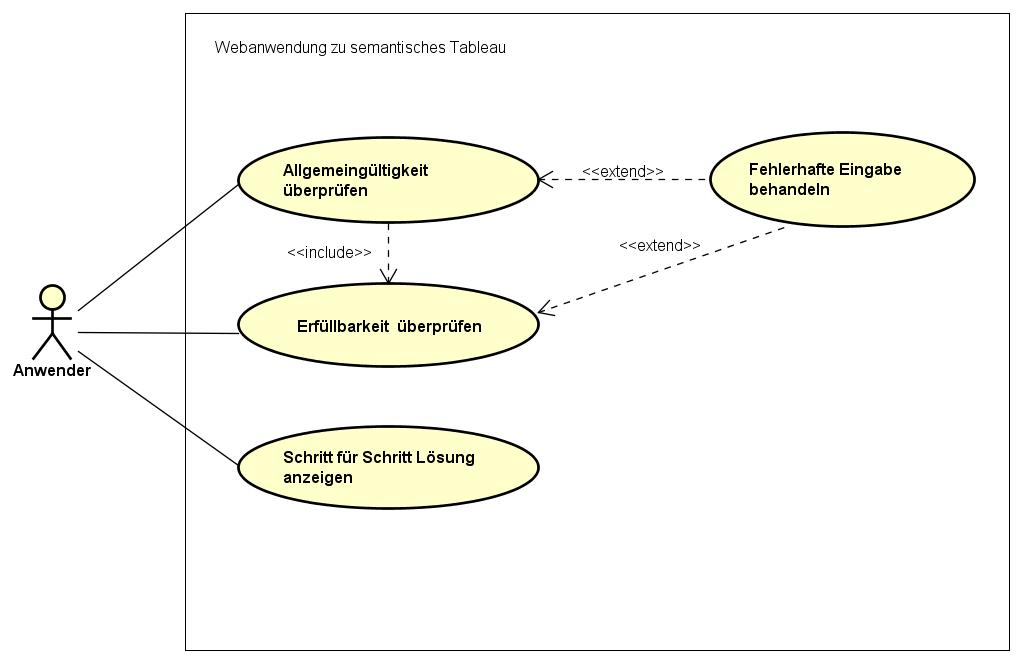
\includegraphics[width=1.0\textwidth]{UsecaseDiagram.jpg}
\caption[Anwendungsfalldiagramm]{Anwendungsfalldiagramm}\label{fig:Anwendungsfalldiagramm}
\end{figure}

\subsection{Anwendungsfallbeschreibung}
\begin{itemize}


%\subsubsection{Anwendungsfall:``Allgemeingültigkeit überprüfen''}
\item \textit{\textbf{Anwendungsfall: ``Allgemeingültigkeit überprüfen''}}

\textbf{Akteure:}

Anwender (initiiert den Anwendungsfall)\\

\textbf{Auslöser:}

Anwender drückt auf ``Tautologie''\\

\textbf{Anfangsbedingungen:}

Der Anwender hat eine Eingabe ins Eingabefeld eingegeben.\\

\textbf{Ereignisfluss:}
\begin{enumerate}
\item Das System prüft, ob die Eingabe ein wohlgeformter Ausdruck der Aussagenlogik ist. 
\item Das System erstellt die Negation der Eingabeformel.
\item Das System zeigt die Darstellung von der Negation der Eingabeformel als Baumstruktur in dem GUI an.
\item Das System initiiert ``Erfüllbarkeit überprüfen'' um zu prüfen, ob die Negation der Eingabeformel erfüllbar ist.
\item Wenn dies erfolgreich ist, erstellt das System das Ergebnis, sodass die Eingabeformel nicht allgemeingültig ist. Wenn nicht, erstellt das System das Ergebnis, sodass die Eingabeformel allgemeingültig ist.
\item Das System zeigt die Darstellung des Tableaus an.
\end{enumerate}

\textbf{Abschlussbedingungen:}

Der Anwender hat entweder das Ergebnis oder eine Systemmeldung über eine fehlerhafte Eingabe erhalten.\\
	
%\subsubsection{Anwendungsfall:``Erfüllbarkeit überprüfen''}
\item \textit{\textbf{Anwendungsfall: ``Erfüllbarkeit überprüfen''}}

\textbf{Akteure:}

Anwender (initiiert den Anwendungsfall)\\

\textbf{Auslöser:}

Anwender drückt auf ``Erfüllbarkeit''\\

\textbf{Anfangsbedingungen:}

Der Anwender hat eine Eingabe ins Eingabefeld eingegeben.\\
 
\textbf{Ereignisfluss:}
\begin{enumerate}
\item Das System prüft, ob die Eingabe ein wohlgeformter Ausdruck der Aussagenlogik ist. 
\item Das System zeigt die Eingabeformel-Darstellung als Baumstruktur in dem GUI an.
\item Das System prüft, ob die Eingabeformel mittels Tableau-Verfahren erfüllbar ist und erstellt das Ergebnis.
\item Das System zeigt die Darstellung des Tableaus an.
\end{enumerate}

\textbf{Abschlussbedingungen:}

Der Anwender hat entweder das Ergebnis oder eine Systemmeldung über eine fehlerhafte Eingabe erhalten.\\

%\subsubsection{Anwendungsfall: ``Schritt für Schritt Lösung auswählen''}
\item \textit{\textbf{Anwendungsfall: ``Schritt für Schritt Lösung anzeigen''}}

\textbf{Akteure:}

Anwender (initiiert den Anwendungsfall)\\

\textbf{Auslöser:}

Anwender drückt auf ``Schritt für Schritt Lösung''\\

\textbf{Anfangsbedingungen:}

Anwender hat ``Erfüllbarkeit'' oder ``Tautologie'' gedrückt.\\

\textbf{Ereignisfluss:}
\begin{enumerate}
\addtolength{\itemindent}{0cm}
\item Das System öffnet ein Pop-up Fenster für die Schritt für Schritt Lösung.
\addtolength{\itemindent}{1cm}
\item  Der Anwender drückt auf ``Nächste Schritt'' um den nächsten Schritt der Lösung anzuzeigen.
\item  Der Anwender drückt auf ``$\times$'' Symbol um das Pop-up Fenster zu schließen.
\addtolength{\itemindent}{0cm}
\end{enumerate}
\begin{enumerate}
  \setcounter{enumi}{3}
 \item Das System schließt das Pop-up Fenster.
\end{enumerate}

\textbf{Abschlussbedingungen:}
Pop-up Fenster ist geschlossen. Der Anwender kann die vorherige Formel nochmal prüfen oder eine neue Formel eingeben.\\

%\textbf{Anwendungsfall:}  "Tableau anzeigen"
%\textbf{Akteure:}
%- System (initiiert den Anwendungsfall)
%-Google Chart Tools (stellt das Tableau dar)
%\textbf{Auslöser:}
%Das System initiiert " Tableau darstellen " zur Darstellung des Tableaus.
%\textbf{Anfangsbedingungen:}
%Das System hat das Tableau erstellt.
%\textbf{Ereignisfluss:}
%1.	Das System prüft, ob die Eingabe ein wohlgeformter Ausdruck der Aussagenlogik ist. 
%2.	Das System prüft, ob die Eingabe Formel mittels Tableau-Verfahren erfüllbar ist und erstellt das Ergebnis.
%3.	Das System initiiert " Tableau darstellen " zur Darstellung des Tableaus.
%\textbf{Abschlussbedingungen:}
%Die Tableau-Darstellung müssen innerhalb von 5 Sekunden bereitgestellt werden können.
%\textbf{Qualitätsanforderung:}

%\subsubsection{Anwendungsfall: ``Fehlerhafte Eingabe behandeln''}
\item \textit{\textbf{Anwendungsfall: ``Fehlerhafte Eingabe behandeln''}}

\textbf{Akteure:}

System (initiiert den Anwendungsfall)\\

\textbf{Auslöser:}

Dieser Anwendungsfall erweitert die Anwendungsfälle ``Allgemeingültigkeit überprüfe'' und ``Erfüllbarkeit überprüfen''. Es wird vom System initiiert, sobald die Eingabe nicht ein wohlgeformter Ausdruck der Aussagenlogik ist.\\

\textbf{Anfangsbedingungen:}

Anwender hat eine fehlerhafte Eingabe eingegeben.\\

\textbf{Ereignisfluss:}
\begin{enumerate}
\item Das System gibt eine Systemmeldung aus.
\end{enumerate}

\textbf{Abschlussbedingungen:}

Der Anwender erhält eine Systemmeldung und kann die Eingabe korrigieren.\\

\end{itemize}

%	\section{Anforderungsanalyse}
\subsection{Anwendungsfalldiagramm}
\begin{figure}[ !h] \centering
%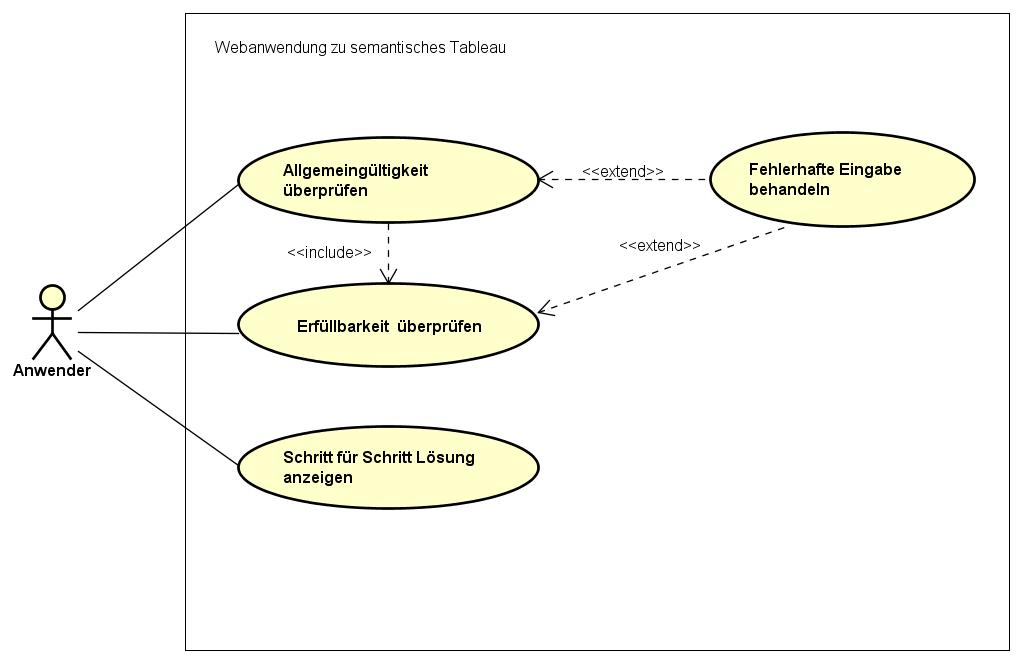
\includegraphics[width=1.0\textwidth,draft=\DraftMode]{UsecaseDiagram}
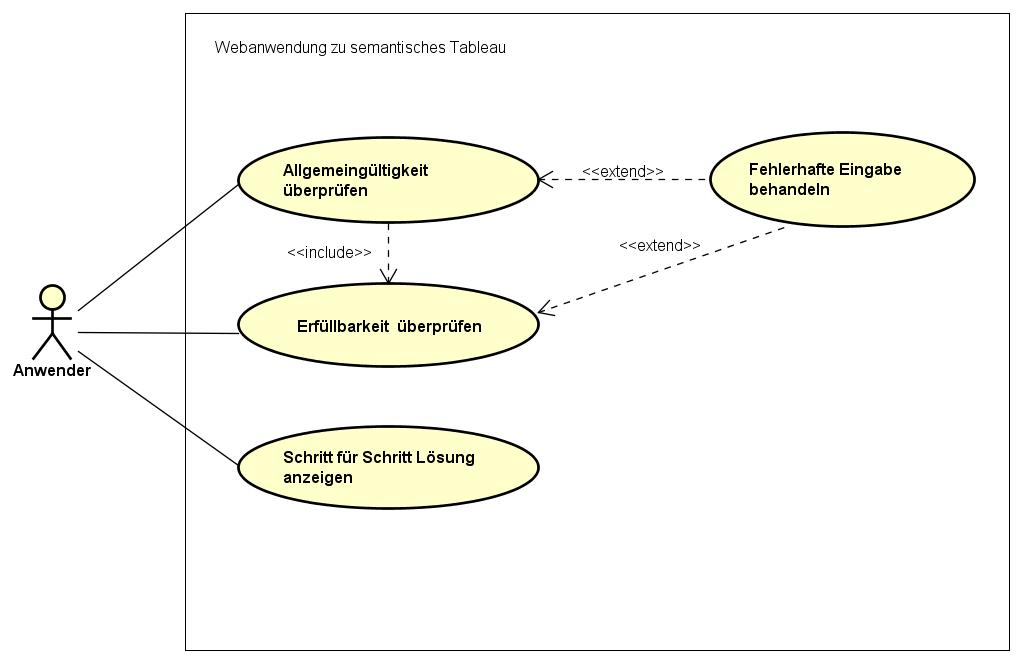
\includegraphics[width=1.0\textwidth]{UsecaseDiagram.jpg}
\caption[Anwendungsfalldiagramm]{Anwendungsfalldiagramm}\label{fig:Anwendungsfalldiagramm}
\end{figure}

\subsection{Anwendungsfallbeschreibung}
\begin{itemize}


%\subsubsection{Anwendungsfall:``Allgemeingültigkeit überprüfen''}
\item \textit{\textbf{Anwendungsfall: ``Allgemeingültigkeit überprüfen''}}

\textbf{Akteure:}

Anwender (initiiert den Anwendungsfall)\\

\textbf{Auslöser:}

Anwender drückt auf ``Tautologie''\\

\textbf{Anfangsbedingungen:}

Der Anwender hat eine Eingabe ins Eingabefeld eingegeben.\\

\textbf{Ereignisfluss:}
\begin{enumerate}
\item Das System prüft, ob die Eingabe ein wohlgeformter Ausdruck der Aussagenlogik ist. 
\item Das System erstellt die Negation der Eingabeformel.
\item Das System zeigt die Darstellung von der Negation der Eingabeformel als Baumstruktur in dem GUI an.
\item Das System initiiert ``Erfüllbarkeit überprüfen'' um zu prüfen, ob die Negation der Eingabeformel erfüllbar ist.
\item Wenn dies erfolgreich ist, erstellt das System das Ergebnis, sodass die Eingabeformel nicht allgemeingültig ist. Wenn nicht, erstellt das System das Ergebnis, sodass die Eingabeformel allgemeingültig ist.
\item Das System zeigt die Darstellung des Tableaus an.
\end{enumerate}

\textbf{Abschlussbedingungen:}

Der Anwender hat entweder das Ergebnis oder eine Systemmeldung über eine fehlerhafte Eingabe erhalten.\\
	
%\subsubsection{Anwendungsfall:``Erfüllbarkeit überprüfen''}
\item \textit{\textbf{Anwendungsfall: ``Erfüllbarkeit überprüfen''}}

\textbf{Akteure:}

Anwender (initiiert den Anwendungsfall)\\

\textbf{Auslöser:}

Anwender drückt auf ``Erfüllbarkeit''\\

\textbf{Anfangsbedingungen:}

Der Anwender hat eine Eingabe ins Eingabefeld eingegeben.\\
 
\textbf{Ereignisfluss:}
\begin{enumerate}
\item Das System prüft, ob die Eingabe ein wohlgeformter Ausdruck der Aussagenlogik ist. 
\item Das System zeigt die Eingabeformel-Darstellung als Baumstruktur in dem GUI an.
\item Das System prüft, ob die Eingabeformel mittels Tableau-Verfahren erfüllbar ist und erstellt das Ergebnis.
\item Das System zeigt die Darstellung des Tableaus an.
\end{enumerate}

\textbf{Abschlussbedingungen:}

Der Anwender hat entweder das Ergebnis oder eine Systemmeldung über eine fehlerhafte Eingabe erhalten.\\

%\subsubsection{Anwendungsfall: ``Schritt für Schritt Lösung auswählen''}
\item \textit{\textbf{Anwendungsfall: ``Schritt für Schritt Lösung anzeigen''}}

\textbf{Akteure:}

Anwender (initiiert den Anwendungsfall)\\

\textbf{Auslöser:}

Anwender drückt auf ``Schritt für Schritt Lösung''\\

\textbf{Anfangsbedingungen:}

Anwender hat ``Erfüllbarkeit'' oder ``Tautologie'' gedrückt.\\

\textbf{Ereignisfluss:}
\begin{enumerate}
\addtolength{\itemindent}{0cm}
\item Das System öffnet ein Pop-up Fenster für die Schritt für Schritt Lösung.
\addtolength{\itemindent}{1cm}
\item  Der Anwender drückt auf ``Nächste Schritt'' um den nächsten Schritt der Lösung anzuzeigen.
\item  Der Anwender drückt auf ``$\times$'' Symbol um das Pop-up Fenster zu schließen.
\addtolength{\itemindent}{0cm}
\end{enumerate}
\begin{enumerate}
  \setcounter{enumi}{3}
 \item Das System schließt das Pop-up Fenster.
\end{enumerate}

\textbf{Abschlussbedingungen:}
Pop-up Fenster ist geschlossen. Der Anwender kann die vorherige Formel nochmal prüfen oder eine neue Formel eingeben.\\

%\textbf{Anwendungsfall:}  "Tableau anzeigen"
%\textbf{Akteure:}
%- System (initiiert den Anwendungsfall)
%-Google Chart Tools (stellt das Tableau dar)
%\textbf{Auslöser:}
%Das System initiiert " Tableau darstellen " zur Darstellung des Tableaus.
%\textbf{Anfangsbedingungen:}
%Das System hat das Tableau erstellt.
%\textbf{Ereignisfluss:}
%1.	Das System prüft, ob die Eingabe ein wohlgeformter Ausdruck der Aussagenlogik ist. 
%2.	Das System prüft, ob die Eingabe Formel mittels Tableau-Verfahren erfüllbar ist und erstellt das Ergebnis.
%3.	Das System initiiert " Tableau darstellen " zur Darstellung des Tableaus.
%\textbf{Abschlussbedingungen:}
%Die Tableau-Darstellung müssen innerhalb von 5 Sekunden bereitgestellt werden können.
%\textbf{Qualitätsanforderung:}

%\subsubsection{Anwendungsfall: ``Fehlerhafte Eingabe behandeln''}
\item \textit{\textbf{Anwendungsfall: ``Fehlerhafte Eingabe behandeln''}}

\textbf{Akteure:}

System (initiiert den Anwendungsfall)\\

\textbf{Auslöser:}

Dieser Anwendungsfall erweitert die Anwendungsfälle ``Allgemeingültigkeit überprüfe'' und ``Erfüllbarkeit überprüfen''. Es wird vom System initiiert, sobald die Eingabe nicht ein wohlgeformter Ausdruck der Aussagenlogik ist.\\

\textbf{Anfangsbedingungen:}

Anwender hat eine fehlerhafte Eingabe eingegeben.\\

\textbf{Ereignisfluss:}
\begin{enumerate}
\item Das System gibt eine Systemmeldung aus.
\end{enumerate}

\textbf{Abschlussbedingungen:}

Der Anwender erhält eine Systemmeldung und kann die Eingabe korrigieren.\\

\end{itemize}

%\chapter{Grundlagen der Aussagenlogik}\label{sec:Grundlagen}

%In diesem Kapitel werden wir uns mit der Grundlagen der Aussagenlogik beschäftigen.
In diesem Kapitel werden die Grundlagen der Aussagenlogik behandelt. Die Aussagenlogik ist ein Zweig der formalen Logik, der die Beziehungen zwischen Aussagen und Aussagenverbindungen untersucht. Aussagen sind abstrakte Begriffe, auch Propositionen genannt, die in der Alltagssprache durch Sätze ausgedrückt werden. Dabei kommt es in der Aussagenlogik nicht auf den konkreten Inhalt der Aussagen an, sondern nur auf die Entscheidung, ob eine Aussage wahr oder falsch ist.

\begin{ex} \label{Beispiel 4.0} \end{ex}
\begin{enumerate}
\item Der Mars ist ein Planet. 
\item  Der Mond ist ein Planet. 
\end{enumerate}

drücken zwei verschiedene Aussagen aus, wovon die erste wahr und die zweite falsch ist.






%\cleardoublepage
\chapter{Grundlagen der Aussagenlogik}\label{sec:Grundlagen}

%In diesem Kapitel werden wir uns mit der Grundlagen der Aussagenlogik beschäftigen.
In diesem Kapitel werden die Grundlagen der Aussagenlogik behandelt. Die Aussagenlogik ist ein Zweig der formalen Logik, der die Beziehungen zwischen Aussagen und Aussagenverbindungen untersucht. Aussagen sind abstrakte Begriffe, auch Propositionen genannt, die in der Alltagssprache durch Sätze ausgedrückt werden. Dabei kommt es in der Aussagenlogik nicht auf den konkreten Inhalt der Aussagen an, sondern nur auf die Entscheidung, ob eine Aussage wahr oder falsch ist.

\begin{ex} \label{Beispiel 4.0} \end{ex}
\begin{enumerate}
\item Der Mars ist ein Planet. 
\item  Der Mond ist ein Planet. 
\end{enumerate}

drücken zwei verschiedene Aussagen aus, wovon die erste wahr und die zweite falsch ist.






%	\section{Syntax der Aussagenlogik}
%Zur Darstellung von Aussagen in einer (für die Mathematik notwendigen) präzisen Struktur repräsentieren wir atomare Aussagen durch Großbuchstaben und Kombinationsmöglichkeiten von Aussagen durch spezielle Symbole. 
In diesem Abschnitt wird die Syntax von Aussagen exakt spezifiziert, damit ist festgelegt,
%welche mathematischen Zeichenketten Aussagen beschreiben und welche nicht. 
welche der aus den Grundelementen bildbaren Zeichenfolgen zulässig oder ``wohlgeformt'' sind und welche nicht.


\subsection{Alphabet der Aussagenlogik}
\begin{defi}Alphabet der Aussagenlogik\label{Definition 2.1}\end{defi}Das Alphabet der Aussagenlogik ist einer Menge von erlaubten Zeichen oder Symbolen und besteht aus:
\begin{itemize}
\item Aussagenvariablen: $p, q, r, s, t \ldots$
\item Junktoren: 
\begin{align*}
Negation  &\ \neg\\
Disjunktion &\ \vee\\  
Konjuktion &\ \wedge \\  
Implikation &\ \rightarrow\\      
Äquivalenz &\ \leftrightarrow\\ 
Exklusives \ Oder &\ \oplus\\  
Nor &\ \downarrow\\   
Nand &\ \uparrow\\
\end{align*}
\item Konstanten: $true$ und $false$\cite{Schenke}
\item Hilfssymbolen: $(,)$ 
\end{itemize}

\subsection{Syntax aussagenlogischer Formeln}
Die folgende Regeln bestimmt welche Zeichenketten, die von dem oberem Alphabet gebildet werden, wohlgeformte Ausdrücke (Formeln) sind, z.B während $(p \rightarrow q)$ eine aussagenlogische Formel ist, ist die $(\wedge p) q \vee)$ keine aussagenlogische Formel.
\begin{defi}\label{Definition 2.1} Formationsregeln\end{defi}
\begin{enumerate}
\item \label{formationsregeln_1}eine Aussagenvariable (atomare Aussage) ist eine Formel.
\item \label{formationsregeln_2}ist $A$ eine aussagenlogische Formel, dann ist auch $\neg A$ eine aussagenlogische Formel.
\item \label{formationsregeln_3}sind $A$ und $B$ aussagenlogische Formeln, dann sind
\begin{enumerate}
\item \label{formationsregeln_3_1}$(A \wedge B)$  
\item \label{formationsregeln_3_2} $(A \vee B)$  
\item $(A \rightarrow B)$   
\item $(A \leftrightarrow B)$      
\item $(A  \oplus B)$      
\item $(A \downarrow B)$      
\item $(A \uparrow B)$   
\end{enumerate}
ebenfalls aussagenlogische Formeln
\item \label{formationsregeln_4}Ein Ausdruck ist nur dann eine aussagenlogische Formel, wenn er durch Anwendung der oben­stehenden Regeln konstruiert werden kann.
\end{enumerate}

Um nachzuweisen, dass bestimmte Zeichenketten  keine wohlgeformten Formel sind, kann man auch beweisen, dass wohlgeformte Formel bestimmte Eigenschaften haben müssen. Wenn diese Zeichenkette eine dieser Eigenschaften nicht
erfüllt, so kann sie auch keine Formel sein.
\begin{bem}\label{AussagenEigenschaften}\cite{Dreiseitl}\end{bem} 
Solche Eigenschaften von Formeln sind etwa:
\begin{itemize}
\item Es gibt ebenso viele öffnende wie schließende Klammern,
\item links und rechts von jedem der Junktoren $\wedge$ und $\vee$ steht eine Formel,
\item eine Formel endet nie mit einem Junktor.
\end{itemize}

\begin{ex}\label{Beispiel 2.1}\end{ex}
Seien $p$, $q$ aussagenlogische Formeln. 
%(¬(p ∧ q) ⇒ (q∨¬q))
Die Zeichenkette $\neg(p \wedge q)$ ist eine Formel, da diese aus den Bildungsregeln \eqref{formationsregeln_1},\eqref{formationsregeln_3_1} und \eqref{formationsregeln_2}  zusammengesetzt werden können.

%((p ∧ ∨q))
Die Zeichenkette $((p \wedge \vee q))$ ist keine Formel, da $\vee q$ (rechts von $p \wedge$) und auch $p \wedge$ (links von $\vee q$) keine Formeln sind.\cite{Dreiseitl}


\subsection{Bindungskonventionen} \label{subsec:Bindungskonventionen}
Die Klammern um die Ausdrücke sind wichtig, weil durch sie die Reihenfolge der semantischen Auswertung geregelt wird, z.B Die Formel $(p \vee q) \wedge r$ wird anders ausgewertet als $p \vee (q \wedge r)$. Da viele Klammern Formeln unübersichtlich werden lassen, vereinbart man analog wie in der elementaren Arithmetik ``Punktrechnung geht vor Strichrechnung'' die folgende Bindungsregeln(von hoch nach niedrig):
\begin{align*}
\neg\\
\wedge, \uparrow\\
\vee, \downarrow\\
\rightarrow\\
\leftrightarrow, \oplus
\end{align*}

%Zusätzliche Klammern können immer verwendet werden, um eine Formel zu verdeutlichen: $(p \vee q) \wedge (q \vee r)$. Die Booleschen Operatoren $\wedge$, $\vee$, $\leftrightarrow$, $\oplus$ sind assoziativ. Daher wird man häufig Klammern in Formeln auslassen, in denen diese Operatoren wiederholt vorkommen: $p \vee q \vee r \vee s$. Beachtet man, dass $\rightarrow$, $\downarrow$, $\uparrow$ nicht assoziativ sind. Daher müssen Klammern verwendet werden, um Verwechslungen zu vermeiden. Obwohl angenommen wird, dass der Implikationsoperator rechts assoziativ ist, so dass $p \rightarrow q \rightarrow r$ eindeutig $p \rightarrow (q \rightarrow r)$ bedeutet, schreibt man die Formel mit Klammern, um eine Verwechslung mit $(p \rightarrow q) \rightarrow r$ zu vermeiden.


\subsection{Baum-Notation von Formeln}
Es ist oft vorteilhaft, sich die Struktur einer Formel $A$ (wie sie durch ihre Unterformeln aufgebaut ist) als einen Syntax-Baum mit Wurzel vorzustellen, dessen Blätter mit den atomaren Aussagen von $A$ und dessen innere Knoten mit geeigneten Junktoren markiert sind. Dabei stimmt die Stelligkeit des markierenden Junktors mit der Anzahl der Kinder überein.
%
%\begin{itemize}
%\item	Eine Formel ist ein mit einer $\neg$ gekennzeichneter Knoten mit einem einzelnen Kind, das eine Formel ist.
%\item	Eine Formel ist ein durch einen der binären Operatoren beschrifteter Knoten mit zwei Kindern, die beide Formeln sind.
%\end{itemize}
%
%%• Eine Formel ist ein Knoten, der mit einem ¬ gekennzeichnet, dann einen einzelnen Kind, das auch eine Formel ist, hat. 
%%• Eine Formel ist ein Knoten, der durch einen der binären Operatoren beschriftet, dann zwei Kindern, die beide auch Formeln sind, hat.

\begin{defi}Formeln als Bäume\label{Definition 2.2}\cite{Ben-Ari} \end{defi}Eine Formel in der Aussagenlogik ist ein rekursiv definierter Baum:
\begin{enumerate}
\item Eine Formel ist ein Blatt, das durch eine atomare Aussage gekennzeichnet ist.
\item Eine Formel ist ein mit einer $\neg$ gekennzeichneter Knoten mit einem einzelnen Kind, das eine Formel ist.
\item Eine Formel ist ein durch einen der binären Operatoren beschrifteter Knoten mit zwei Kindern, die beide Formeln sind.
\end{enumerate}
Abbildung \ref{Abb. 2.1} zeigt Baum-Notation von $p \rightarrow p \leftrightarrow \neg p \rightarrow \neg q $:
\begin {figure}[h]
\begin{center}
\definecolor{ududff}{rgb}{0.30196078431372547,0.30196078431372547,1}
\definecolor{uuuuuu}{rgb}{0,0,0}
\begin{tikzpicture}[line cap=round,line join=round,>=triangle 45,x=1cm,y=1cm]

\clip(-3.5,-6.5) rectangle (3.38,0.68);
\draw [line width=1pt] (0,0)-- (-2,-2);
\draw [line width=1pt] (0,0)-- (2,-2);
\draw [line width=1pt] (-2,-2.5)-- (-3,-4);
\draw [line width=1pt] (-2,-2.5)-- (-1,-4);
\draw [line width=1pt] (2,-2.5)-- (1,-4);
\draw [line width=1pt] (2,-2.5)-- (3,-4);
\draw [line width=1pt] (1,-4.5)-- (1,-6);
\draw [line width=1pt] (3,-4.5)-- (3,-6);
\begin{small}
\draw[color=uuuuuu] (0,0.33) node {$\leftrightarrow$};
\draw[color=uuuuuu] (-2,-2.25) node {$\rightarrow$};
\draw[color=uuuuuu] (2,-2.25) node {$\rightarrow$};;
\draw[color=uuuuuu] (-3,-4.25) node {$p$};
\draw[color=uuuuuu] (-1,-4.25) node {$q$};
\draw[color=uuuuuu] (1,-4.25) node {$\neg$};
\draw[color=uuuuuu] (3,-4.25) node {$\neg$};
\draw[color=uuuuuu] (1,-6.25) node {$p$};
\draw[color=uuuuuu] (3,-6.25) node {$q$};
\end{small}
\end{tikzpicture}
\end{center}
\caption[Beispiel Konstruktion für eine Formel]{Formel $p \rightarrow p \leftrightarrow \neg p \rightarrow \neg q $ ist ein Baum}	
\label{Abb. 2.1}
\end{figure}

\begin{bem}\label{FormelAlsString}\end{bem}
So wie man Ausdrücke als Strings schreibt (lineare Folgen von Symbolen), kann man Formeln als Strings schreiben. Die einer Formel zugeordnete Zeichenfolge kann durch eine Inorder-Traversierung des Baums erhalten werden.


\subsection{Operator-Notation}\label{subsec:Notation}
Die Bücher über mathematische Logik benutzen eine stark variierende Notation für die Booleschen Operatoren. Außerdem erscheinen die Operatoren in Programmiersprachen mit einer anderen Notation als es in Mathematikbüchern verwendet wird. Folgende Tabelle zeigt einige dieser alternativen Notationen.

\begin{table}[h]

			\begin{center}
			\begin{tabular}{ccc}
			\hline
			\textbf{Junktor} & \textbf{Literatur} & \textbf{Java}\\
			\hline
			\hline
			$\neg$ &$\sim$& !\\
			\hline
			$\wedge$  & \& & \&, \&\&  \\
			\hline
			$\vee$ &  & |,||\\
			\hline
			$\rightarrow$  & $\supset,\Rightarrow$ & \\
			\hline
			$\leftrightarrow$ & $\equiv,\Leftrightarrow$ & \\
			\hline
			$\oplus$ &$\not\equiv$ &$\mbox{\textasciicircum}$ \\
			\hline
			\end{tabular}
			\end{center}
			\caption[Notationen der Booleschen Operatoren]{Alternative Notationen\cite{Ben-Ari}}
			\label{Notationen}
			\end{table}
			
\subsection{Eine formale Grammatik für Formeln}\label{subsec:FormelGrammatik}

%Dieser Unterabschnitt setzt Vertrautheit mit formalen Grammatiken voraus. Anstatt Formeln als Bäume zu definieren, können sie als Strings definiert werden, die eine kontextfreie formale Grammatik generieren.

Dieser Unterabschnitt setzt Vertrautheit mit formalen Grammatiken voraus. Anstatt Formeln als Bäume zu definieren, können sie als Strings, die über einer kontextfreien formalen Grammatik generiert werden, definiert werden.

\begin{defi} \label{Definition 2.13}Kontextfreien Grammatik für Formel \end{defi} Formeln in der Aussagenlogik werden aus der kontextfreien Grammatik abgeleitet, deren Terminals sind \cite{Ben-Ari}:
\begin{itemize}
\item  Eine unbegrenzte Menge von Symbolen $\mathcal{P}$, die atomare Propositionen heißen.
\item  Die Booleschen Operatoren in Definition \ref{Definition 2.1}.
\end{itemize}
Die Produktionen der Grammatik sind:
\begin{align*}
fml &:: = p \ für \ jedes \ p \in  \mathcal{P}\\
fml &:: = \neg fml\\
fml &:: = fml \  op \ fml\\
op &:: = \vee | \wedge | \rightarrow  |\leftrightarrow | \oplus | \uparrow | \downarrow
\end{align*}


%Eine Formel ist ein Wort, das aus dem Nichtterminal $fml$ abgeleitet werden kann. Die Menge von allen Formeln, die von der Grammatik abgeleitet werden können, sind mit $\mathcal{F}$ bezeichnet. Ableitungen von Strings (Wörtern) in einer formalen Grammatik können als Bäume dargestellt werden (Hopcroft et al., 2006, Abschn. 4.3). Das durch eine Ableitung erzeugte Wort kann gelesen werden von den Blättern von links nach rechts.






















%\begin{ex} \label{Beispiel 2.14} \end{ex} Hier ist eine Herleitung der Formel p $\rightarrow$    q $\leftrightarrow$ $\neg$p $\rightarrow$   $\neg$q in der Aussagenlogik; Der Baum, der seine Ableitung darstellt, ist in Abb. \ref{Abb. 2.2} dargestellt.
%
%\begin{figure}[ !h] \centering												
% 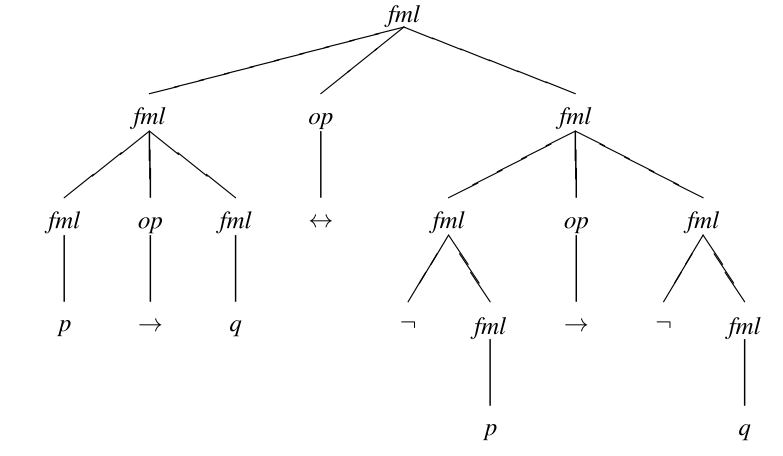
\includegraphics[width=1.0\textwidth]{A3}					
% \caption[Ableitungsbaum für p $\rightarrow$   q $\leftrightarrow$ $\neg$p $\rightarrow$  $\neg$q]{Derivation tree for p $\rightarrow$   q $\leftrightarrow$ $\neg$p $\rightarrow$  $\neg$q}					
% \label{Abb. 2.2} 
%\end{figure}
%
%\begin{align*}
%&fml\\
%&fml \  op \ fml\\
%&fml \leftrightarrow fml\\
%&fml \  op \  fml \leftrightarrow fml\\
%&fml \rightarrow fml \leftrightarrow fml\\
%&p \rightarrow fml \leftrightarrow fml\\
%&p \rightarrow q \leftrightarrow fml\\
%&p \rightarrow q \leftrightarrow fml  \  op \  fml\\
%&p \rightarrow q \leftrightarrow fml \rightarrow fml\\
%&p \rightarrow q \leftrightarrow \neg fml \rightarrow fml\\
%&p \rightarrow q \leftrightarrow \neg p \rightarrow fml\\
%&p \rightarrow q \leftrightarrow \neg p \rightarrow \neg q
%\end{align*}
%
%
%
%%\begin{figure}[ !h] \centering												
%% 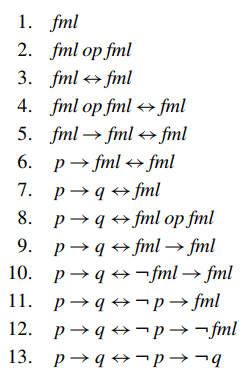
\includegraphics[width=0.3\textwidth]{A0}									
%% \label{Abb. A0}
%%\end{figure}
%
%
%Die in Abschn. \ref{sssec:num1} kann zur Auflösung von Mehrdeutigkeiten verwendet werden. Wir können die Grammatik ändern, um Klammern einzuführen: 
%\begin{align*}
%fml &:: = (\neg \  fml)\\
%fml &:: = (fml \  op \  fml)
%\end{align*}
%und dann die Präzedenz verwenden, um ihre Anzahl zu reduzieren.
%

	\section{Syntax der Aussagenlogik}
%Zur Darstellung von Aussagen in einer (für die Mathematik notwendigen) präzisen Struktur repräsentieren wir atomare Aussagen durch Großbuchstaben und Kombinationsmöglichkeiten von Aussagen durch spezielle Symbole. 
In diesem Abschnitt wird die Syntax von Aussagen exakt spezifiziert, damit ist festgelegt,
%welche mathematischen Zeichenketten Aussagen beschreiben und welche nicht. 
welche der aus den Grundelementen bildbaren Zeichenfolgen zulässig oder ``wohlgeformt'' sind und welche nicht.


\subsection{Alphabet der Aussagenlogik}
\begin{defi}Alphabet der Aussagenlogik\label{Definition 2.1}\end{defi}Das Alphabet der Aussagenlogik ist einer Menge von erlaubten Zeichen oder Symbolen und besteht aus:
\begin{itemize}
\item Aussagenvariablen: $p, q, r, s, t \ldots$
\item Junktoren: 
\begin{align*}
Negation  &\ \neg\\
Disjunktion &\ \vee\\  
Konjuktion &\ \wedge \\  
Implikation &\ \rightarrow\\      
Äquivalenz &\ \leftrightarrow\\ 
Exklusives \ Oder &\ \oplus\\  
Nor &\ \downarrow\\   
Nand &\ \uparrow\\
\end{align*}
\item Konstanten: $true$ und $false$\cite{Schenke}
\item Hilfssymbolen: $(,)$ 
\end{itemize}

\subsection{Syntax aussagenlogischer Formeln}
Die folgende Regeln bestimmt welche Zeichenketten, die von dem oberem Alphabet gebildet werden, wohlgeformte Ausdrücke (Formeln) sind, z.B während $(p \rightarrow q)$ eine aussagenlogische Formel ist, ist die $(\wedge p) q \vee)$ keine aussagenlogische Formel.
\begin{defi}\label{Definition 2.1} Formationsregeln\end{defi}
\begin{enumerate}
\item \label{formationsregeln_1}eine Aussagenvariable (atomare Aussage) ist eine Formel.
\item \label{formationsregeln_2}ist $A$ eine aussagenlogische Formel, dann ist auch $\neg A$ eine aussagenlogische Formel.
\item \label{formationsregeln_3}sind $A$ und $B$ aussagenlogische Formeln, dann sind
\begin{enumerate}
\item \label{formationsregeln_3_1}$(A \wedge B)$  
\item \label{formationsregeln_3_2} $(A \vee B)$  
\item $(A \rightarrow B)$   
\item $(A \leftrightarrow B)$      
\item $(A  \oplus B)$      
\item $(A \downarrow B)$      
\item $(A \uparrow B)$   
\end{enumerate}
ebenfalls aussagenlogische Formeln
\item \label{formationsregeln_4}Ein Ausdruck ist nur dann eine aussagenlogische Formel, wenn er durch Anwendung der oben­stehenden Regeln konstruiert werden kann.
\end{enumerate}

Um nachzuweisen, dass bestimmte Zeichenketten  keine wohlgeformten Formel sind, kann man auch beweisen, dass wohlgeformte Formel bestimmte Eigenschaften haben müssen. Wenn diese Zeichenkette eine dieser Eigenschaften nicht
erfüllt, so kann sie auch keine Formel sein.
\begin{bem}\label{AussagenEigenschaften}\cite{Dreiseitl}\end{bem} 
Solche Eigenschaften von Formeln sind etwa:
\begin{itemize}
\item Es gibt ebenso viele öffnende wie schließende Klammern,
\item links und rechts von jedem der Junktoren $\wedge$ und $\vee$ steht eine Formel,
\item eine Formel endet nie mit einem Junktor.
\end{itemize}

\begin{ex}\label{Beispiel 2.1}\end{ex}
Seien $p$, $q$ aussagenlogische Formeln. 
%(¬(p ∧ q) ⇒ (q∨¬q))
Die Zeichenkette $\neg(p \wedge q)$ ist eine Formel, da diese aus den Bildungsregeln \eqref{formationsregeln_1},\eqref{formationsregeln_3_1} und \eqref{formationsregeln_2}  zusammengesetzt werden können.

%((p ∧ ∨q))
Die Zeichenkette $((p \wedge \vee q))$ ist keine Formel, da $\vee q$ (rechts von $p \wedge$) und auch $p \wedge$ (links von $\vee q$) keine Formeln sind.\cite{Dreiseitl}


\subsection{Bindungskonventionen} \label{subsec:Bindungskonventionen}
Die Klammern um die Ausdrücke sind wichtig, weil durch sie die Reihenfolge der semantischen Auswertung geregelt wird, z.B Die Formel $(p \vee q) \wedge r$ wird anders ausgewertet als $p \vee (q \wedge r)$. Da viele Klammern Formeln unübersichtlich werden lassen, vereinbart man analog wie in der elementaren Arithmetik ``Punktrechnung geht vor Strichrechnung'' die folgende Bindungsregeln(von hoch nach niedrig):
\begin{align*}
\neg\\
\wedge, \uparrow\\
\vee, \downarrow\\
\rightarrow\\
\leftrightarrow, \oplus
\end{align*}

%Zusätzliche Klammern können immer verwendet werden, um eine Formel zu verdeutlichen: $(p \vee q) \wedge (q \vee r)$. Die Booleschen Operatoren $\wedge$, $\vee$, $\leftrightarrow$, $\oplus$ sind assoziativ. Daher wird man häufig Klammern in Formeln auslassen, in denen diese Operatoren wiederholt vorkommen: $p \vee q \vee r \vee s$. Beachtet man, dass $\rightarrow$, $\downarrow$, $\uparrow$ nicht assoziativ sind. Daher müssen Klammern verwendet werden, um Verwechslungen zu vermeiden. Obwohl angenommen wird, dass der Implikationsoperator rechts assoziativ ist, so dass $p \rightarrow q \rightarrow r$ eindeutig $p \rightarrow (q \rightarrow r)$ bedeutet, schreibt man die Formel mit Klammern, um eine Verwechslung mit $(p \rightarrow q) \rightarrow r$ zu vermeiden.


\subsection{Baum-Notation von Formeln}
Es ist oft vorteilhaft, sich die Struktur einer Formel $A$ (wie sie durch ihre Unterformeln aufgebaut ist) als einen Syntax-Baum mit Wurzel vorzustellen, dessen Blätter mit den atomaren Aussagen von $A$ und dessen innere Knoten mit geeigneten Junktoren markiert sind. Dabei stimmt die Stelligkeit des markierenden Junktors mit der Anzahl der Kinder überein.
%
%\begin{itemize}
%\item	Eine Formel ist ein mit einer $\neg$ gekennzeichneter Knoten mit einem einzelnen Kind, das eine Formel ist.
%\item	Eine Formel ist ein durch einen der binären Operatoren beschrifteter Knoten mit zwei Kindern, die beide Formeln sind.
%\end{itemize}
%
%%• Eine Formel ist ein Knoten, der mit einem ¬ gekennzeichnet, dann einen einzelnen Kind, das auch eine Formel ist, hat. 
%%• Eine Formel ist ein Knoten, der durch einen der binären Operatoren beschriftet, dann zwei Kindern, die beide auch Formeln sind, hat.

\begin{defi}Formeln als Bäume\label{Definition 2.2}\cite{Ben-Ari} \end{defi}Eine Formel in der Aussagenlogik ist ein rekursiv definierter Baum:
\begin{enumerate}
\item Eine Formel ist ein Blatt, das durch eine atomare Aussage gekennzeichnet ist.
\item Eine Formel ist ein mit einer $\neg$ gekennzeichneter Knoten mit einem einzelnen Kind, das eine Formel ist.
\item Eine Formel ist ein durch einen der binären Operatoren beschrifteter Knoten mit zwei Kindern, die beide Formeln sind.
\end{enumerate}
Abbildung \ref{Abb. 2.1} zeigt Baum-Notation von $p \rightarrow p \leftrightarrow \neg p \rightarrow \neg q $:
\begin {figure}[h]
\begin{center}
\definecolor{ududff}{rgb}{0.30196078431372547,0.30196078431372547,1}
\definecolor{uuuuuu}{rgb}{0,0,0}
\begin{tikzpicture}[line cap=round,line join=round,>=triangle 45,x=1cm,y=1cm]

\clip(-3.5,-6.5) rectangle (3.38,0.68);
\draw [line width=1pt] (0,0)-- (-2,-2);
\draw [line width=1pt] (0,0)-- (2,-2);
\draw [line width=1pt] (-2,-2.5)-- (-3,-4);
\draw [line width=1pt] (-2,-2.5)-- (-1,-4);
\draw [line width=1pt] (2,-2.5)-- (1,-4);
\draw [line width=1pt] (2,-2.5)-- (3,-4);
\draw [line width=1pt] (1,-4.5)-- (1,-6);
\draw [line width=1pt] (3,-4.5)-- (3,-6);
\begin{small}
\draw[color=uuuuuu] (0,0.33) node {$\leftrightarrow$};
\draw[color=uuuuuu] (-2,-2.25) node {$\rightarrow$};
\draw[color=uuuuuu] (2,-2.25) node {$\rightarrow$};;
\draw[color=uuuuuu] (-3,-4.25) node {$p$};
\draw[color=uuuuuu] (-1,-4.25) node {$q$};
\draw[color=uuuuuu] (1,-4.25) node {$\neg$};
\draw[color=uuuuuu] (3,-4.25) node {$\neg$};
\draw[color=uuuuuu] (1,-6.25) node {$p$};
\draw[color=uuuuuu] (3,-6.25) node {$q$};
\end{small}
\end{tikzpicture}
\end{center}
\caption[Beispiel Konstruktion für eine Formel]{Formel $p \rightarrow p \leftrightarrow \neg p \rightarrow \neg q $ ist ein Baum}	
\label{Abb. 2.1}
\end{figure}

\begin{bem}\label{FormelAlsString}\end{bem}
So wie man Ausdrücke als Strings schreibt (lineare Folgen von Symbolen), kann man Formeln als Strings schreiben. Die einer Formel zugeordnete Zeichenfolge kann durch eine Inorder-Traversierung des Baums erhalten werden.


\subsection{Operator-Notation}\label{subsec:Notation}
Die Bücher über mathematische Logik benutzen eine stark variierende Notation für die Booleschen Operatoren. Außerdem erscheinen die Operatoren in Programmiersprachen mit einer anderen Notation als es in Mathematikbüchern verwendet wird. Folgende Tabelle zeigt einige dieser alternativen Notationen.

\begin{table}[h]

			\begin{center}
			\begin{tabular}{ccc}
			\hline
			\textbf{Junktor} & \textbf{Literatur} & \textbf{Java}\\
			\hline
			\hline
			$\neg$ &$\sim$& !\\
			\hline
			$\wedge$  & \& & \&, \&\&  \\
			\hline
			$\vee$ &  & |,||\\
			\hline
			$\rightarrow$  & $\supset,\Rightarrow$ & \\
			\hline
			$\leftrightarrow$ & $\equiv,\Leftrightarrow$ & \\
			\hline
			$\oplus$ &$\not\equiv$ &$\mbox{\textasciicircum}$ \\
			\hline
			\end{tabular}
			\end{center}
			\caption[Notationen der Booleschen Operatoren]{Alternative Notationen\cite{Ben-Ari}}
			\label{Notationen}
			\end{table}
			
\subsection{Eine formale Grammatik für Formeln}\label{subsec:FormelGrammatik}

%Dieser Unterabschnitt setzt Vertrautheit mit formalen Grammatiken voraus. Anstatt Formeln als Bäume zu definieren, können sie als Strings definiert werden, die eine kontextfreie formale Grammatik generieren.

Dieser Unterabschnitt setzt Vertrautheit mit formalen Grammatiken voraus. Anstatt Formeln als Bäume zu definieren, können sie als Strings, die über einer kontextfreien formalen Grammatik generiert werden, definiert werden.

\begin{defi} \label{Definition 2.13}Kontextfreien Grammatik für Formel \end{defi} Formeln in der Aussagenlogik werden aus der kontextfreien Grammatik abgeleitet, deren Terminals sind \cite{Ben-Ari}:
\begin{itemize}
\item  Eine unbegrenzte Menge von Symbolen $\mathcal{P}$, die atomare Propositionen heißen.
\item  Die Booleschen Operatoren in Definition \ref{Definition 2.1}.
\end{itemize}
Die Produktionen der Grammatik sind:
\begin{align*}
fml &:: = p \ für \ jedes \ p \in  \mathcal{P}\\
fml &:: = \neg fml\\
fml &:: = fml \  op \ fml\\
op &:: = \vee | \wedge | \rightarrow  |\leftrightarrow | \oplus | \uparrow | \downarrow
\end{align*}


%Eine Formel ist ein Wort, das aus dem Nichtterminal $fml$ abgeleitet werden kann. Die Menge von allen Formeln, die von der Grammatik abgeleitet werden können, sind mit $\mathcal{F}$ bezeichnet. Ableitungen von Strings (Wörtern) in einer formalen Grammatik können als Bäume dargestellt werden (Hopcroft et al., 2006, Abschn. 4.3). Das durch eine Ableitung erzeugte Wort kann gelesen werden von den Blättern von links nach rechts.






















%\begin{ex} \label{Beispiel 2.14} \end{ex} Hier ist eine Herleitung der Formel p $\rightarrow$    q $\leftrightarrow$ $\neg$p $\rightarrow$   $\neg$q in der Aussagenlogik; Der Baum, der seine Ableitung darstellt, ist in Abb. \ref{Abb. 2.2} dargestellt.
%
%\begin{figure}[ !h] \centering												
% 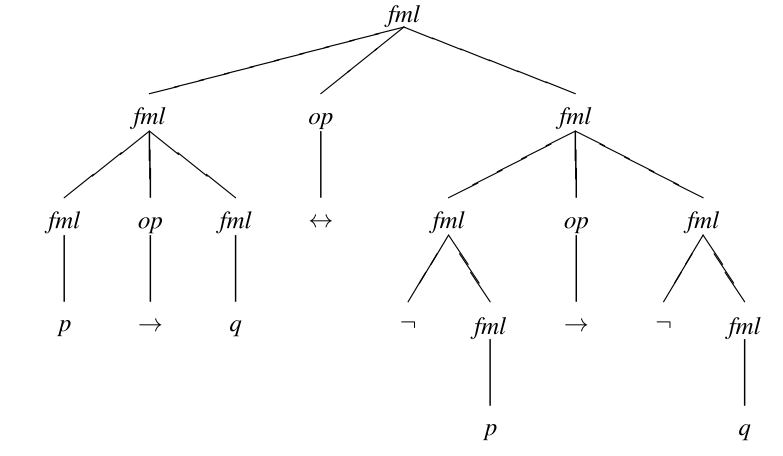
\includegraphics[width=1.0\textwidth]{A3}					
% \caption[Ableitungsbaum für p $\rightarrow$   q $\leftrightarrow$ $\neg$p $\rightarrow$  $\neg$q]{Derivation tree for p $\rightarrow$   q $\leftrightarrow$ $\neg$p $\rightarrow$  $\neg$q}					
% \label{Abb. 2.2} 
%\end{figure}
%
%\begin{align*}
%&fml\\
%&fml \  op \ fml\\
%&fml \leftrightarrow fml\\
%&fml \  op \  fml \leftrightarrow fml\\
%&fml \rightarrow fml \leftrightarrow fml\\
%&p \rightarrow fml \leftrightarrow fml\\
%&p \rightarrow q \leftrightarrow fml\\
%&p \rightarrow q \leftrightarrow fml  \  op \  fml\\
%&p \rightarrow q \leftrightarrow fml \rightarrow fml\\
%&p \rightarrow q \leftrightarrow \neg fml \rightarrow fml\\
%&p \rightarrow q \leftrightarrow \neg p \rightarrow fml\\
%&p \rightarrow q \leftrightarrow \neg p \rightarrow \neg q
%\end{align*}
%
%
%
%%\begin{figure}[ !h] \centering												
%% 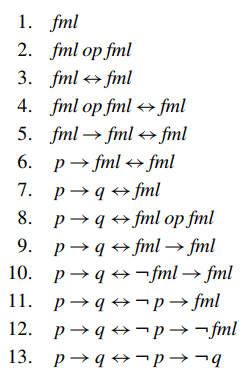
\includegraphics[width=0.3\textwidth]{A0}									
%% \label{Abb. A0}
%%\end{figure}
%
%
%Die in Abschn. \ref{sssec:num1} kann zur Auflösung von Mehrdeutigkeiten verwendet werden. Wir können die Grammatik ändern, um Klammern einzuführen: 
%\begin{align*}
%fml &:: = (\neg \  fml)\\
%fml &:: = (fml \  op \  fml)
%\end{align*}
%und dann die Präzedenz verwenden, um ihre Anzahl zu reduzieren.
%

%	\section{Semantik der Aussagenlogik}

Aussagen sind wahr oder falsch. Von einer aussagenlogischen Formel kann man das erst dann sagen, wenn man (zumindest) den in ihr vorkommenden Variablen einen Wahrheitswert zugeordnet hat.

\begin{defi} Belegung atomarer Aussagen\cite{Schaefer} \end{defi}Sei  $A$ eine aussagenlogische Formel und sei $\mathcal{P}_A$ die Menge der in der Formel $A$ vorkommenden atomaren Aussagen. Eine Belegung $v$ (von ``valuation'') für $A$ ist eine Abbildung $v$ : $\mathcal{P}_A \rightarrow \{ wahr,falsch \}$, die jeder atomaren Aussage der Formel $A$ einen Wahrheitswert zuweist.


\begin{defi}Wahrheitswert einer Formel\end{defi} Sei  $A$ eine aussagenlogische Formel und sei $v$ eine Belegung der in $\mathcal{A}$ vorkommenden atomaren Aussagen.  $v_{\mathcal{P}_A} (A)$  , der Wahrheitswert von $A$ unter  $\mathcal{P}_A$ ist induktiv auf der Struktur von $A$ definiert, wie in Abb. \ref{Abb. 2.3} gezeigt.
\begin{figure}[ !h] \centering		
\begin{align*}
v_\mathcal{P}(A)  &= \mathcal{P}_A (A)\hspace{0.7cm} \mbox{ falls A eine atomare Formel ist}\\
v_\mathcal{P}(\neg A)  &= \left\{ \begin{array}{lll}
wahr & \mbox{falls}& v_\mathcal{P}(A) = falsch \\ 
falsch & \mbox{sonst} & \\
\end{array}\right.\\
v_\mathcal{P}(A_1 \vee A_2)  &= \left\{ \begin{array}{lll}
wahr & \mbox{falls}& v_\mathcal{P}(A_1) = wahr \ und \ v_\mathcal{P}(A_2) = wahr \\ 
falsch & \mbox{sonst} & \\
\end{array}\right.\\
v_\mathcal{P}(A_1 \wedge A_2)  &= \left\{ \begin{array}{lll}
falsch & \mbox{falls}& v_\mathcal{P}(A_1) = falsch \ und \ v_\mathcal{P}(A_2) = falsch \\ 
wahr & \mbox{sonst} & \\
\end{array}\right.\\
v_\mathcal{P}(A_1 \rightarrow A_2)  &= \left\{ \begin{array}{lll}
falsch & \mbox{falls}& v_\mathcal{P}(A_1) = wahr \ und \ v_\mathcal{P}(A_2) = falsch \\ 
wahr & \mbox{sonst} & \\
\end{array}\right.\\
v_\mathcal{P}(A_1 \uparrow A_2)  &= \left\{ \begin{array}{lll}
falsch & \mbox{falls}& v_\mathcal{P}(A_1) = wahr \ und \ v_\mathcal{P}(A_2) = wahr \\ 
wahr & \mbox{sonst} & \\
\end{array}\right.\\
v_\mathcal{P}(A_1 \downarrow A_2)  &= \left\{ \begin{array}{lll}
wahr & \mbox{falls}& v_\mathcal{P}(A_1) = falsch \ und \ v_\mathcal{P}(A_2) = falsch \\ 
falsch & \mbox{sonst} & \\
\end{array}\right.\\
v_\mathcal{P}(A_1 \leftrightarrow A_2)  &= \left\{ \begin{array}{lll}
wahr & \mbox{falls}& v_\mathcal{P}(A_1) = v_\mathcal{P}(A_2) \\ 
falsch & \mbox{sonst} & \\
\end{array}\right.\\
v_\mathcal{P}(A_1 \oplus A_2)  &= \left\{ \begin{array}{lll}
wahr & \mbox{falls}& v_\mathcal{P}(A_1) \neq v_\mathcal{P}(A_2) \\ 
falsch & \mbox{sonst} & \\
\end{array}\right.\\
\end{align*}
 \caption[Wahrheitswerte von Formeln]{Wahrheitswerte von Formeln}	 
 \label{Abb. 2.3}
\end{figure}

In Abb. \ref{Abb. 2.3} wird $v_{\mathcal{P}_A} (A)$ mit $v_\mathcal{P}(A)$ abgekürzt. Die Abkürzung $\mathcal{P}$ für $\mathcal{P}_A$ wird immer dann verwendet, wenn die Formel aus dem Kontext klar ist.
\section{Erfüllbarkeit und Tautologien}
Grundsätzlich kann man Formeln danach klassifizieren, ob überhaupt passende Belegungen existieren, die sie wahr bzw. falsch machen.
\begin{defi} Erfüllbarkeit, Gültigkeit , Tautologie \label{Definition 2.38} \end{defi}  Eine Formel $A$ heißt
\begin{itemize}																					
\item erfüllbar, falls sie unter wenigstens einer Belegung wahr ist;
\item gültig, allgemeingültig oder Tautologie, falls sie unter allen Belegung wahr ist;
\item unerfüllbar, falls es keine passende Belegung gibt, sodass diese wahr ist.
\end{itemize}
\begin{bem} \label{Satz 2.39} \end{bem}Eine Formel $A$ ist gültig genau dann wenn $\neg A$ unerfüllbar ist.


%	\section{Semantik der Aussagenlogik}

Aussagen sind wahr oder falsch. Von einer aussagenlogischen Formel kann man das erst dann sagen, wenn man (zumindest) den in ihr vorkommenden Variablen einen Wahrheitswert zugeordnet hat.

\begin{defi} Belegung atomarer Aussagen\cite{Schaefer} \end{defi}Sei  $A$ eine aussagenlogische Formel und sei $\mathcal{P}_A$ die Menge der in der Formel $A$ vorkommenden atomaren Aussagen. Eine Belegung $v$ (von ``valuation'') für $A$ ist eine Abbildung $v$ : $\mathcal{P}_A \rightarrow \{ wahr,falsch \}$, die jeder atomaren Aussage der Formel $A$ einen Wahrheitswert zuweist.


\begin{defi}Wahrheitswert einer Formel\end{defi} Sei  $A$ eine aussagenlogische Formel und sei $v$ eine Belegung der in $\mathcal{A}$ vorkommenden atomaren Aussagen.  $v_{\mathcal{P}_A} (A)$  , der Wahrheitswert von $A$ unter  $\mathcal{P}_A$ ist induktiv auf der Struktur von $A$ definiert, wie in Abb. \ref{Abb. 2.3} gezeigt.
\begin{figure}[ !h] \centering		
\begin{align*}
v_\mathcal{P}(A)  &= \mathcal{P}_A (A)\hspace{0.7cm} \mbox{ falls A eine atomare Formel ist}\\
v_\mathcal{P}(\neg A)  &= \left\{ \begin{array}{lll}
wahr & \mbox{falls}& v_\mathcal{P}(A) = falsch \\ 
falsch & \mbox{sonst} & \\
\end{array}\right.\\
v_\mathcal{P}(A_1 \vee A_2)  &= \left\{ \begin{array}{lll}
wahr & \mbox{falls}& v_\mathcal{P}(A_1) = wahr \ und \ v_\mathcal{P}(A_2) = wahr \\ 
falsch & \mbox{sonst} & \\
\end{array}\right.\\
v_\mathcal{P}(A_1 \wedge A_2)  &= \left\{ \begin{array}{lll}
falsch & \mbox{falls}& v_\mathcal{P}(A_1) = falsch \ und \ v_\mathcal{P}(A_2) = falsch \\ 
wahr & \mbox{sonst} & \\
\end{array}\right.\\
v_\mathcal{P}(A_1 \rightarrow A_2)  &= \left\{ \begin{array}{lll}
falsch & \mbox{falls}& v_\mathcal{P}(A_1) = wahr \ und \ v_\mathcal{P}(A_2) = falsch \\ 
wahr & \mbox{sonst} & \\
\end{array}\right.\\
v_\mathcal{P}(A_1 \uparrow A_2)  &= \left\{ \begin{array}{lll}
falsch & \mbox{falls}& v_\mathcal{P}(A_1) = wahr \ und \ v_\mathcal{P}(A_2) = wahr \\ 
wahr & \mbox{sonst} & \\
\end{array}\right.\\
v_\mathcal{P}(A_1 \downarrow A_2)  &= \left\{ \begin{array}{lll}
wahr & \mbox{falls}& v_\mathcal{P}(A_1) = falsch \ und \ v_\mathcal{P}(A_2) = falsch \\ 
falsch & \mbox{sonst} & \\
\end{array}\right.\\
v_\mathcal{P}(A_1 \leftrightarrow A_2)  &= \left\{ \begin{array}{lll}
wahr & \mbox{falls}& v_\mathcal{P}(A_1) = v_\mathcal{P}(A_2) \\ 
falsch & \mbox{sonst} & \\
\end{array}\right.\\
v_\mathcal{P}(A_1 \oplus A_2)  &= \left\{ \begin{array}{lll}
wahr & \mbox{falls}& v_\mathcal{P}(A_1) \neq v_\mathcal{P}(A_2) \\ 
falsch & \mbox{sonst} & \\
\end{array}\right.\\
\end{align*}
 \caption[Wahrheitswerte von Formeln]{Wahrheitswerte von Formeln}	 
 \label{Abb. 2.3}
\end{figure}

In Abb. \ref{Abb. 2.3} wird $v_{\mathcal{P}_A} (A)$ mit $v_\mathcal{P}(A)$ abgekürzt. Die Abkürzung $\mathcal{P}$ für $\mathcal{P}_A$ wird immer dann verwendet, wenn die Formel aus dem Kontext klar ist.
\section{Erfüllbarkeit und Tautologien}
Grundsätzlich kann man Formeln danach klassifizieren, ob überhaupt passende Belegungen existieren, die sie wahr bzw. falsch machen.
\begin{defi} Erfüllbarkeit, Gültigkeit , Tautologie \label{Definition 2.38} \end{defi}  Eine Formel $A$ heißt
\begin{itemize}																					
\item erfüllbar, falls sie unter wenigstens einer Belegung wahr ist;
\item gültig, allgemeingültig oder Tautologie, falls sie unter allen Belegung wahr ist;
\item unerfüllbar, falls es keine passende Belegung gibt, sodass diese wahr ist.
\end{itemize}
\begin{bem} \label{Satz 2.39} \end{bem}Eine Formel $A$ ist gültig genau dann wenn $\neg A$ unerfüllbar ist.


%	\section{Erfüllbarkeit und Tautologien}
Grundsätzlich kann man Formeln danach klassifizieren, ob überhaupt passende Belegungen
existieren, die sie wahr oder falsch machen.
\begin{defi} \label{Definition 2.38} \end{defi} 
Eine Formel A heißt: 
\begin{itemize}																					
\item \textit{erfüllbar}, falls sie unter wenigstens einer Belegung wahr ist.
\item \textit{Tautologie}, falls sie für jede passende Belegung wahr ist.
\item \textit{unerfüllbar}, falls es keine passende Belegung wahr gibt.
\end{itemize}
\begin{sa} \label{Satz 2.39} \end{sa}
Eine Formel $A$ ist gültig genau dann wenn $\neg A$ unerfüllbar ist.
	\section{Erfüllbarkeit und Tautologien}
Grundsätzlich kann man Formeln danach klassifizieren, ob überhaupt passende Belegungen
existieren, die sie wahr oder falsch machen.
\begin{defi} \label{Definition 2.38} \end{defi} 
Eine Formel A heißt: 
\begin{itemize}																					
\item \textit{erfüllbar}, falls sie unter wenigstens einer Belegung wahr ist.
\item \textit{Tautologie}, falls sie für jede passende Belegung wahr ist.
\item \textit{unerfüllbar}, falls es keine passende Belegung wahr gibt.
\end{itemize}
\begin{sa} \label{Satz 2.39} \end{sa}
Eine Formel $A$ ist gültig genau dann wenn $\neg A$ unerfüllbar ist.
	\section{Semantisches Tableau}
%
%Die Methode der semantischen Tableaus ist eine effiziente Entscheidungsprozedur für Erfüllbarkeit (und Dualität) in der Aussagenlogik.
% 
%Das Prinzip hinter semantischen Tableaus ist sehr einfach: Sucht man nach einem Modell, das die Interpretation erfüllt, indem man die Formel in mehrere Mengen von Atomen und Negationen zerlegt. Eine Menge von Atomen und Negationen von Atomen ist erfüllbar, wenn die Menge kein Atom $p$ und seine Negation $\neg p$ enthält. Die Formel ist erfüllbar, wenn eine dieser Mengen erfüllbar ist. Die Formel ist unerfüllbar, wenn keine Mengen erfüllbar ist d.h seine Negation eine Tautologie. 

Das Prinzip hinter semantischen Tableaus ist sehr einfach: Man sucht nach einem Modell, das die Interpretation erfüllt, indem man die Formel in mehreren Mengen von Literalen zerlegt. Eine Menge von Literalen ist erfüllbar, wenn die Menge kein komplementäres Literalpaar enthält. Die Formel ist erfüllbar, wenn eine dieser Mengen erfüllbar ist. Die Formel ist unerfüllbar, wenn keine Mengen erfüllbar sind, d.h seine Negation eine Tautologie ist.

\begin{defi} \label{Definition 2.57} Literal und komplementäres Literalpaar\cite{Ben-Ari}\end{defi} 
Ein Literal ist ein Atom oder die Negation eines Atoms. Ein Atom ist ein positives Literal und die Negation eines Atoms ist ein negatives Literal. Für jedes Atom $p$ ist $\{p, \neg p\}$ ein komplementäres Literalpaar.

Für jede Formel $A$ ist $\{A, \neg A\}$ ein komplementäres Formelpaar. $A$ ist das Komplement von $\neg A$ und $\neg A$ ist das Komplement von $A$.

\begin{ex} \label{Beispiel 2.58} \end{ex} In der Menge der Literale $ \{ \neg p, q, r, \neg r \} $ sind $q$ und $r$ positive Literale, während $\neg p$ und $\neg r$ negative Literale sind. Die Menge enthält das komplementäre Literalpaar $ \{ r, \neg r \}$.
 
%\begin{bem} \label{Satz 2.60 } Eine Menge von Literalen ist genau dann erfüllbar, wenn sie kein komplementäres Literalpaar enthält.\end{bem}
 
 
%\begin{sa} \label{Satz 2.60 } \end{sa}Eine Menge von Literalen ist genau dann erfüllbar, wenn sie vorhanden ist enthält kein komplementäres Literalpaar.

In der Methode der semantischen Tableaus bezeichnen Mengen von Formeln Knoten eines Baumes, wobei jeder Pfad im Baum die Formeln darstellen, die in einer möglichen Interpretation erfüllt sein müssen.

\begin{defi} \label{Def.Tableau} Konstruktion von semantischen Tableaus\end{defi} 
\begin{itemize}
\item Ein aussagenlogisches Tableau ist ein markierter Baum. Jeder Knoten ist mit einer Menge von Formeln markiert.
\item Die Eingabeformel ist an der Wurzel. 
%\footnote{\url{https://www.ki.informatik.uni-frankfurt.de/lehre/SS2008/AD/folien/ded-fol3.pdf}}
\item Jeder Knoten hat einen oder zwei untergeordnete Knoten, abhängig davon, wie eine Formel, die den Knoten kennzeichnet, zerlegt wird. Dadurch, dass ein Knoten mit $\alpha$-Formel gekennzeichnet wird, hat er nur einen untergeordneten Knoten, ansonsten hat er zwei Knoten. Die Klassifizierung von $\alpha$- und $\beta$-Formeln wird in der Tabelle \ref{Abb. 2.8} definiert.
\item Die Blätter sind durch eine Menge von Literalen markiert.
\item Ein Blatt, das durch eine Menge von Literalen markiert ist, die ein komplementäres Paar von Literalen enthält, ist mit geschlossen ($\times$) markiert
\item Ein Blatt, das durch eine Menge von Literalen markiert ist, die kein komplementäres Paar von Literalen enthält, ist mit offen ($\odot$) markiert. 
\item Ein Tableau ist geschlossen, wenn alle seine Blätter als geschlossen markiert sind. Ansonsten (wenn ein Blatt als offen markiert ist), ist es offen.\cite{Ben-Ari}
\end{itemize}


Abbildung \ref{Abb. 2.7} zeigt semantische Tableaus für die Formeln:

$A = p\wedge (\neg q \vee \neg p)$ und $B = (p \vee q) \wedge  (\neg p \wedge  \neg q)$.

\begin {figure}[h]
\vspace{1cm}
\begin{center}
\definecolor{ududff}{rgb}{0.30196078431372547,0.30196078431372547,1}
\definecolor{uuuuuu}{rgb}{0,0,0}
\begin{tikzpicture}[line cap=round,line join=round,>=triangle 45,x=1cm,y=1cm]
\clip(-13.0,-8.0) rectangle (-2.0,-0.5);
\draw [->,>=stealth,line width=1pt] (-11,-2) -- (-11,-3);
\draw [->,>=stealth,line width=1pt] (-11.5,-4) -- (-12.5,-4.5);
\draw [->,>=stealth,line width=1pt] (-10.5,-4) -- (-9.5,-4.5);
\draw [->,>=stealth,line width=1pt] (-4.5,-2) -- (-4.5,-3);
\draw [->,>=stealth,line width=1pt] (-4.5,-4) -- (-4.5,-5);
\draw [->,>=stealth,line width=1pt] (-5,-6) -- (-6,-6.5);
\draw [->,>=stealth,line width=1pt] (-4,-6) -- (-3,-6.5);
\begin{small}
\draw[color=uuuuuu] (-11,-0.8) node {$\textbf{A}$};
\draw[color=uuuuuu] (-11,-1.5) node {$p \wedge (\neg q \vee \neg p)$};
\draw[color=uuuuuu] (-11,-3.5) node {$p, \neg q \vee \neg p$};
\draw[color=uuuuuu] (-12.5,-5) node {$p,\neg q$};
\draw[color=uuuuuu] (-12.5,-5.5) node {$\odot$};
\draw[color=uuuuuu] (-9.5,-5) node {$p, \neg p$};
\draw[color=uuuuuu] (-9.5,-5.5) node {$\times$};
\draw[color=uuuuuu] (-4.5,-0.8) node {$\textbf{B}$};
\draw[color=uuuuuu] (-4.5,-1.5) node {$(p\vee q)\wedge(\neg p \wedge \neg q)$};
\draw[color=uuuuuu] (-4.5,-3.5) node {$p\vee q, \neg p \wedge \neg q$};
\draw[color=uuuuuu] (-4.5,-5.5) node {$p\vee q, \neg p, \neg q$};
\draw[color=uuuuuu] (-6,-7.0) node {$p,\neg p, \neg q$};
\draw[color=uuuuuu] (-6,-7.5) node {$\times$};
\draw[color=uuuuuu](-3,-7.0) node {$q,\neg p,\neg q$};
\draw[color=uuuuuu] (-3,-7.5) node {$\times$};
\end{small}
\end{tikzpicture}
\end{center}
\caption[Beispiel Konstruktion für semantische Tableaus]{Semantische Tableaus für $A = p\wedge (\neg q \vee \neg p)$ und $B = (p \vee q) \wedge  (\neg p \wedge  \neg q)$}
\label{Abb. 2.7}
\vspace{1cm}
\end{figure}

Die Tableau-Konstruktion ist nicht eindeutig. Abbildung \ref{Abb. 2.6} ist ein weiteres Tableau für die Formel $B$. Die Unterschiede zwischen dem Tableau in der Abbildung \ref{Abb. 2.7} und in der Abbildung \ref{Abb. 2.6} sind, dass in dem ersten Tableau die Belegung für $\neg p \wedge \neg q$ gesucht werden, bevor die für $p \vee q$  gesucht wird. Das erste Tableau enthält weniger Knoten, was zeigt, dass \textit{Konjunktionen vor Disjunktionen} vorzuziehen sind.

\begin {figure}[!h]
\begin{center}
\vspace{1cm}
\definecolor{ududff}{rgb}{0.30196078431372547,0.30196078431372547,1}
\begin{tikzpicture}[line cap=round,line join=round,>=triangle 45,x=1cm,y=1cm]
\clip(-13.5,-8.0) rectangle (-8.0,-1.3);
\draw [->,>=stealth,line width=1pt] (-11,-2) -- (-11,-3);
\draw [->,>=stealth,line width=1pt] (-11.5,-4) -- (-12.5,-4.5);
\draw [->,>=stealth,line width=1pt] (-10.5,-4) -- (-9.5,-4.5);
\draw [->,>=stealth,line width=1pt] (-12.5,-5.5) -- (-12.5,-6.5);
\draw [->,>=stealth,line width=1pt] (-9.5,-5.5) -- (-9.5,-6.5);
\begin{small}
\draw[color=black]  (-11,-1.5) node {$(p \vee q) \wedge(\neg p \wedge \neg q)$};
\draw[color=black]  (-11,-3.5) node {$p \vee q, \neg p \wedge \neg q$};
\draw[color=black]  (-12.5,-5) node {$p,\neg p \wedge \neg q$};
\draw[color=black]  (-9.5,-5) node {$q, \neg p \wedge \neg q$};
\draw[color=black] (-12.5,-7) node {$p, \neg p, \neg q$};
\draw[color=black] (-9.5,-7) node {$q, \neg p \wedge \neg q$};
\draw[color=black] (-12.5,-7.5) node {$\times$};
\draw[color=black] (-9.5,-7.5) node {$\times$};
\end{small}
\end{tikzpicture}
\end{center}
\caption[Ein weiteres Tableau]{Ein weiteres Tableau für $B$}
\label{Abb. 2.6}

\end{figure}

Eine übersichtliche Darstellung der Regeln für die Erstellung eines semantischen Tableaus kann gegeben werden, wenn \textit{Formeln nach ihrem Hauptoperator klassifiziert} werden (Tabelle \ref{Abb. 2.8}). Wenn \textit{die Formel eine Negation ist, berücksichtigt die Klassifizierung sowohl die Negation als auch den Hauptoperator}. \textit{$\alpha$-Formeln sind konjunktiv} und nur erfüllbar, wenn beide Teilformeln $\alpha_1$ und $\alpha_2$ erfüllt sind, während \textit{$\beta$-Formeln disjunktiv sind} und auch dann erfüllt sind, wenn nur eine der Teilformeln $\beta_1$ oder $\beta_2$ erfüllbar ist.

\begin{table}[h]
\footnotesize
	\begin{center}
			\begin{tabular}{lcccclccc}
			\cline{1-4}
			\cline{6-9}
			\textbf{Nr.}&\textbf{$\alpha$}&\textbf{$\alpha_1$}&\textbf{$\alpha_2$}&   &\textbf{Nr.}&\textbf{$\beta$}&\textbf{$\beta_1$}&\textbf{$\beta_2$}  \\
			\cline{1-4} 
			\cline{6-9}
			
			\textbf{a1}&$\neg \neg A_1$&$A_1$&  &   &&&&\\
			
			\textbf{a2}&$A_1 \wedge A_2$&$A_1$&$A_2$&   &\textbf{b1}&$\neg (B_1 \wedge B_2)$&$\neg B_1$&$\neg B_2$\\
			\textbf{a3}&$\neg (A_1 \vee A_2)$&$\neg A_1$&$\neg A_2$&   &\textbf{b2}&$B_1 \vee B_2 $&$B_1$&$B_2$\\
			
			\textbf{a4}&$\neg (A_1 \rightarrow A_2)$& $A_1$ & $\neg A_2$&   &\textbf{b3}&$(B_1 \rightarrow B_2)$&$\neg B_1$&$B_2$  \\
			
			\textbf{a5}&$\neg(A_1 \uparrow A_2)$& $A_1$&$A_2$&   &\textbf{b4}&$B_1 \uparrow B_2$&$\neg B_1$&$\neg B_2$  \\
			
			\textbf{a6}&$A_1 \downarrow A_2$&$\neg A_1$ & $\neg A_2$&   &\textbf{b5}&$\neg (B_1 \downarrow B_2)$&$B_1$&$B_2$  \\
			
			\textbf{a7}&$A_1 \leftrightarrow A_2$& $A_1 \rightarrow A_2$&$A_2 \rightarrow A_1$&   &\textbf{b6}&$\neg (B_1 \leftrightarrow B_2)$&$\neg (B_1 \rightarrow B_2)$&$\neg (B_2 \rightarrow B_1)$\\
			
			\textbf{a8}&$\neg (A_1 \oplus A_2)$&$A_1 \rightarrow A_2$&$A_2 \rightarrow A_1$&   &\textbf{b7}&$B_1 \oplus B_2$&$\neg (B_1 \rightarrow B_2)$&$\neg (B_2 \rightarrow B_1)$\\
			\cline{1-4} 
			\cline{6-9}			
			\end{tabular}
	\end{center}
	\caption[Klassifizierung von $\alpha$- und $\beta$-Formeln]{Klassifizierung von $\alpha$- und $\beta$-Formeln \cite{Ben-Ari}}
	\label{Abb. 2.8}
\end{table}
		
\vspace{0.5cm}\begin{ex} \label{Beispiel 2.63} \end{ex} Die Formel $p \wedge q$ wird als $\alpha$-Formel klassifiziert, weil sie genau dann gilt, wenn sowohl $p$ als auch $q$ wahr sind. Die Formel $\neg(p\wedge q)$ wird als $\beta$-Formel klassifiziert.
Es ist logisch äquivalent zu $\neg p \vee \neg q$ und ist genau dann wahr, wenn entweder $\neg p$ wahr oder $\neg q$ wahr ist.

Der Algorithmus der Tableau-Konstruktion kann wie folgt formuliert werden:
\begin{al}Konstruktion eines semantischen Tableaus \cite{Schaefer}\label{Algorithmus 2.64} \end{al} 
\textit{Eingabe:} Aussagenlogische Formel $A$.\\
\textit{Ausgabe:} Semantisches Tableau mit markierten Blättern
\begin{enumerate}[wide=0em, leftmargin=*, label=\arabic*, itemsep=0pt, parsep=0pt, font=\scriptsize]
\item \textbf{function} Tableau($A$)
\item \tabto{0.cm} Konstruiere einen Baum mit Formel $A$ als Wurzel.
\item \tabto{0.5cm} \textbf{while} es gibt unmarkierte Blätter \textbf{do} 
\item \tabto{0.5cm} Wähle unmarkiertes Blatt $l$
\item \tabto{1cm}\textbf{if}  Blatt $l$ enthält nur Literale then
\item \tabto{1.5cm} \textbf{if} Blatt $l$ enthält komplementäre Literale oder Konstante \textit{false} \textbf{then}
\item \tabto{2cm} Markiere Blatt $l$ als geschlossen mit $\times$ 
\item \tabto{1.5cm} \textbf{else} 
\item \tabto{2cm} Markiere Blatt $l$ als offen mit $\odot$
\item \tabto{1.5cm} \textbf{end if} 
\item \tabto{1cm} \textbf{else if}  Blatt $l$ enthält $\alpha$-Formel then
\item \tabto{1.5cm} Wähle $\alpha$-Formel $\alpha$
\item \label{TableauAl_13} \tabto{1.5cm} Ermittle Formeln $\alpha_1$ und $\alpha_2$ nach Tabelle \ref{Abb. 2.8} 
\item \tabto{1.5cm} Erzeuge Kind $l'$ von $l$
\item \tabto{1.5cm} Beschrifte $l'$ mit Formeln aus $l$
\item \label{TableauAl_16}\tabto{1.5cm} Ersetze dabei $\alpha$ in $l'$ durch Formeln $\alpha_1$  und $\alpha_2$
\item \tabto{1cm} \textbf{else} 
\item \tabto{1.5cm} Wähle  $\beta$-Formel $\beta$
\item \label{TableauAl_19} \tabto{1.5cm} Ermittle Formeln $\beta_1$ und $\beta_2$ nach Tabelle \ref{Abb. 2.8}
\item \tabto{1.5cm} Erzeuge zwei Kinder $l_1$ und $l_2$ von $l$
\item \tabto{1.5cm} Beschrifte $l_1$ mit Formeln aus $l$
\item \tabto{1.5cm} Ersetze dabei $\beta$ in $l_1$ durch $\beta_1$
\item \tabto{1.5cm} Beschrifte $l_2$ mit Formeln aus $l$
\item \label{TableauAl_24}\tabto{1.5cm} Ersetze dabei $\beta$ in $l_2$ durch $\beta_2$
\item \tabto{1cm} \textbf{end if} 
\item \tabto{0.5cm} \textbf{end while}
\item \tabto{0.5cm} \textbf{return}  Semantisches Tableau
\item \textbf{end function}
\end{enumerate}



%\begin{defi} \label{Definition 2.65} \end{defi} Ein Tableau, dessen Konstruktion beendet wurde, ist ein abgeschlossenes Tableau. Ein abgeschlossenes Tableau wird geschlossen, wenn alle seine Blätter als geschlossen markiert sind. Ansonsten (wenn ein Blatt als offen markiert ist), ist es offen.
%\cleardoublepage	
\chapter{Frameworks}\label{sec:Frameworks}
Dieses Kapitel befasst sich mit den Frameworks für die Umsetzung:
\begin{itemize}
\item Antlr4 (für die Analyse der Eingabe)
\item Bootstrap (für die Gestaltung der Webanwendung)
\item Google Charts (für die Darstellung des Tableaus) 
\item Jasmine (für das automatisierte Testen)
\end{itemize}

	\section{Antlr4}\label{sec:Antlr4}
Um die syntaktische Richtigkeit der Benutzereingabeformel zu prüfen und die Formel in einem Baum-Struktur darstellen zu können (\hyperlink{/LF10/}{/LF10/}), wird ANTLR verwendet.

ANTLR ist ein leistungsfähiger Parser-Generator, mit dem man strukturierte Text- oder Binärdateien lesen, verarbeiten, ausführen oder übersetzen kann. Es wird häufig in der Wissenschaft und der Industrie verwendet, um alle möglichen Sprachen, Werkzeuge und Frameworks zu erstellen. ANTLR ist kostenlos und als ``Open Source'' erhältlich.

Die Twitter-Suche verwendet ANTLR für die Abfrageanalyse mit mehr als 2 Milliarden Abfragen pro Tag. Die Sprachen für Hive und Pig und die Data Warehouse- und Analysesysteme für Hadoop verwenden ANTLR. Lex Machina verwendet ANTLR zur Informationsextraktion aus Rechtstexten. Oracle verwendet ANTLR innerhalb der SQL Developer IDE und seiner Migrationstools. Die NetBeans-IDE analysiert C++ mit ANTLR. Die HQL-Sprache im objektrelationalen Hibernate-Mapping-Framework wird mit ANTLR erstellt.\cite{Parr}

Aus einer formellen Sprachbeschreibung, die als Grammatik bezeichnet wird, generiert ANTLR einen Parser für diese Sprache. Ein Parser liest den vom Lexer in einzelne Token zerteilten Strom ein, prüft diese auf syntaktische Richtigkeit und erstellt daraus Symbol-Gruppen mit hierarchischer Struktur. Die Struktur ist oft ein Baum und wird dann abstrakter Syntaxbaum (AST) oder Parse-tree genannt. ANTLR generiert außerdem automatisch Tree-Walker, mit denen Sie die Knoten dieser Bäume aufrufen können, um anwendungsspezifischen Code auszuführen.

%Der wichtigste Unterschied zwischen ANTLR und anderen Parser-Generatoren wie z.B YACC / Bison ist der Typ der Grammatiken, die diese Tools verarbeiten können. YACC / Bison behandeln LALR-Grammatiken, ANTLR behandelt LL-Grammatiken. YACC / Bison erzeugt tabellengesteuerte Parser, was bedeutet, dass die ``Verarbeitungslogik'' in den Daten des Parserprogramms enthalten ist, nicht so sehr in dem Parsercode. ANTLR erzeugt rekursive Descent-Parser, was bedeutet, dass die ``Verarbeitungslogik'' im Parser-Code enthalten ist, da jede Produktionsregel der Grammatik durch eine Funktion im Parser-Code repräsentiert wird. Der Vorteil ist, dass es einfacher ist zu verstehen, was der Parser tut, indem er seinen Code liest. Außerdem sind rekursive Descent-Parser typischerweise schneller als tabellengesteuerte.\footnote{\url{https://stackoverflow.com/questions/212900/advantages-of-antlr-versus-say-lex-yacc-bison}}. 

Um einen AST zu bekommen, muss man:
\begin{itemize}
\item Eine Lexer- und Parsergrammatik definieren.
\item ANTLR aufrufen: Es generiert einen Lexer und einen Parser in einer Zielsprache (z. B. Java, Python, JavaScript)
\item Den generierten Lexer und Parser verwenden: Rufe Lexer und Parser, dann übergebe den Code. Lexer und Parser werden den Code erkennen und einen AST zurückgeben
\end{itemize}

\subsection{Hauptteilen von ANTLR}
ANTLR besteht eigentlich aus zwei Hauptteilen: dem Werkzeug (Antlr-Tool), mit dem der Lexer und Parser erzeugt wird und der Laufzeit, die für die Ausführung benötigt wird. Das Antlr-Tool ist immer gleich, unabhängig davon, auf welche Sprache abgezielt wird. Es ist ein Java-Programm, das nur für Entwickler benötigt wird. Die Laufzeit (Runtime) ist für jede Sprache unterschiedlich und muss sowohl dem Entwickler als auch dem Benutzer zur Verfügung stehen. Die Runtime kann auf der Seite \url{http://www.antlr.org/download/} heruntergeladen werden. 

Die einzige Voraussetzung für das Antlr-Tool ist, dass mindestens Java 1.7 installiert werden muss. Um dieses Antlr-Tool zu installieren, muss die neueste Version von der offiziellen Website, die im Moment \url{http://www.antlr.org/download/antlr-4.7.1-complete.jar} ist, heruntergeladen werden. Die Ausführliche Anleitung zur Installation wird auf der Seite \url{https://github.com/antlr/antlr4/blob/master/doc/getting-started.md} beschrieben.

Wenn man ANTLR verwendet, beginnt man mit dem Schreiben einer Grammatik, einer Datei mit der Erweiterung \textit{.g4}. Diese Grammatik erhält die Regeln der Sprache, die analysiert wird. Dann verwendet man das Antlr-Tool, um die Dateien, die man in seinem Projekt wirklich braucht, zu erstellen,  wie zB. \textit{antlr4 <Optionen> <Grammatik-Datei-Name.g4>}

Es gibt einige wichtige Optionen, die man bei der Ausführung von Antlr-Tool angeben kann. Man kann die Zielsprache angeben, um einen Parser in Python oder JavaScript oder einem anderen Ziel als Java (das ist das Standardziel) zu erstellen.
ANTLR bietet zwei Tree-Walking-Mechanismen in seiner Laufzeitbibliothek: eine Parser-Tree-Listener-Schnittstelle und eine Parser-Tree-Visitor-Schnittstelle \cite{Parr}. Standardmäßig wird nur der Listener generiert. Um den Visitor zu erstellen, kann man die Befehlszeilenoption \textit{-visitor} verwenden. Eine vollständige Liste der Optionen für das Antlr-Tool kann man auf der Seite \url{https://github.com/antlr/antlr4/blob/master/doc/tool-options.md} finden.


\subsection{ANTLR JavaScript target}
Während der Konfiguration von ANTLR in JavaScript gibt es einige Besonderheiten wie folgt:

\begin{itemize}
\item 	Grammatiken im gleichen Ordner wie die JavaScript-Dateien ablegen.
\item	Die Datei mit der Grammatik muss den gleichen Namen wie die Grammatik haben, die am Anfang der Datei angegeben werden muss.
\item	Der entsprechende JavaScript-Parser kann einfach die richtige Option mit dem Antlr-Tool erstellen.

\textit{antlr4 -Dlanguage = JavaScript Grammatik-Datei-Name.g4}

Damit die Manipulationen erleichtert werden, wird in dieser Arbeit eine \textit{.BAT-Datei} \textit{antlr4.bat} verwendet. Die Datei erhält die Kommando
\begin{lstlisting}[language=HTML,basicstyle=\scriptsize]
	antlr4 -Dlanguage=JavaScript -listener -visitor -encoding UTF-8 FormulaGrammar.g4
\end{lstlisting}
um die Parser, Lexer sowie Listener und Visitor für die \textit{FormulaGrammar.g4} in JavaScript zu generieren.

\item	ANTLR kann sowohl mit \textit{node.js} als auch im Browser verwendet werden. Für den Browser muss man webpack oder \textit{require.js} verwenden um zu vermeiden, dass dutzende Dateien manuell importiert werden müssen.

Im Rahmen diese Bachelorarbeit wird \textit{require.js} gewählt. Das Skript wird von Torben Haase zur Verfügung gestellt und ist nicht Bestandteil der ANTLR JavaScript-Runtime. Dieses Skript kann auf der Seite \url{https://github.com/antlr/antlr4/blob/master/runtime/JavaScript/src/lib/require.js\#L65} heruntergeladen werden.
Angenommen hat man im Stammverzeichnis seiner Website sowohl das Verzeichnis ``antlr4'' als auch ein ``lib'' -Verzeichnis mit ``require.js'', muss man die in denn HTML-Header wie folgt einfügen:

\begin{lstlisting}[language=HTML,basicstyle=\scriptsize]
	<script src='lib/require.js'>
	<script>
		var antlr4 = require('antlr4/index');
	</script>
\end{lstlisting}

\item Die generierten  Lexer und Parser in JavaScript kann wie folgt ausgeführt werden:

\begin{lstlisting}[language=JavaScript,basicstyle=\scriptsize ]
	var antlr4 = require('antlr4');
	var MyGrammarLexer = require('./MyGrammarLexer').MyGrammarLexer;
	var MyGrammarParser = require('./MyGrammarParser').MyGrammarParser;
	var MyGrammarListener = require('./MyGrammarListener').MyGrammarListener;

	var input = "your text to parse here"
	var chars = new antlr4.InputStream(input);
	var lexer = new MyGrammarLexer(chars);
	var tokens  = new antlr4.CommonTokenStream(lexer);
	var parser = new MyGrammarParser(tokens);
	parser.buildParseTrees = true;
	var tree = parser.StartRule();
\end{lstlisting}

Dazu sind \textit{MyGrammarLexer.js, MyGrammarParser.js, MyGrammarListener.js} und \textit{MyGrammarVisitor.js} die generierten Dateien für die Grammatik  ``\textit{MyGrammar}'', die eine Regel ``\textit{StartRule}'' enthält.

\item	Wenn man den Syntaxbaum mit einem benutzerdefinierten Listener besuchen möchte, kann man einen benutzerdefinierten Listener wie folgt erstellen:

\begin{lstlisting}[language=JavaScript,basicstyle=\scriptsize]
	MyGrammarListener = function(ParseTreeListener) {
		// some code here
	}
	// some code here
	MyGrammarListener.prototype.enterKey = function(ctx) {};
	MyGrammarListener.prototype.exitKey = function(ctx) {};
	MyGrammarListener.prototype.enterValue = function(ctx) {};
	MyGrammarListener.prototype.exitValue = function(ctx) {};
\end{lstlisting}

Um benutzerdefiniertes Verhalten bereitzustellen, kann man eine Klasse wie folgt erstellen:

\begin{lstlisting}[language=JavaScript,basicstyle=\scriptsize]
	var KeyPrinter = function() {
		MyGrammarListener.call(this); // inherit default listener
		return this;
	};

	// continue inheriting default listener
	KeyPrinter.prototype = Object.create(MyGrammarListener.prototype);
	KeyPrinter.prototype.constructor = KeyPrinter;

	// override default listener behavior
	KeyPrinter.prototype.exitKey = function(ctx) {
	console.log("Oh, a key!");
	};
\end{lstlisting}

Um diesen Listener auszuführen, fügt man dem obigen Code einfach die folgenden Zeilen hinzu:

\begin{lstlisting}[language=JavaScript,basicstyle=\scriptsize]
	...
	tree = parser.StartRule() // only repeated here for reference
	var printer = new KeyPrinter();
	antlr4.tree.ParseTreeWalker.DEFAULT.walk(printer, tree);
\end{lstlisting}

\end{itemize}
Die Ausführliche Anleitung zur JavaScript Konfiguration kann man auf der Seite \url{https://github.com/antlr/antlr4/blob/master/doc/javascript-target.md} lesen. 
	\section{Bootstrap}
%https://www.internet-exposure.com/blog/standalone-mobile-websites-vs-responsive-design/
Immer mehr Smartphones, Tablets und andere Mobilgeräte werden genutzt, um im Internet zu surfen. Weltweit werden 68 Millionen Google-Suchanfragen pro Stunde auf Mobilgeräten durchgeführt. Laut StatCounter waren im Juli 2018 52,95\% des weltweiten Internetverkehrs auf einem Mobilgerät. Weitere 3,94\% kamen von Tablets \cite{statCounter}. Das bedeutet, dass Mobile Nutzer einen großen Einfluss haben, mit dem man rechnen muss um den langfristigen Erfolg sicherzustellen. Es gibt zwei Optionen zum Erstellen einer für Mobilgeräte optimierten Website. Man kann eine separate mobile Website oder eine Responsive-Website entwickeln.
 
\subsection{Eigenständige mobile Website (Separate mobile Website)}
%Mobile-dedizierte Websites
Separate mobile Websites sind Websites, die speziell für Mobilgeräte entwickelt wurden. Sie leben häufig unter einer separaten URL (z.B. \textit{m.site.de}) und unterscheiden sich von der vollständigen Website. Sie enthalten Funktionen oder Inhalte, die für Mobilgeräte als geeignet erachtet wurden. Häufig sind dies nur einige der auf dem Desktop verfügbaren Komponenten. 
%(muss noch umschreiben)Sie stehen oft im Gegensatz zu Responsive-Websites, die für Mobilgeräte und Desktops in der Regel dieselben Inhalte und Funktionen enthalten, diese jedoch auf Mobilgeräten neu anordnen. 
Eine separate mobile Website bietet Differenzierung von mobilen Inhalten und erstellt ein vollständig mobiles Benutzererlebnis.

%http://todayslocalmedia.com/standalone-mobile-site-vs-mobile-responsive-site/
Das größte Problem mit separaten mobilen Websites besteht darin, dass man zwei separate Websites erstellen und verwalten muss. Wenn man Änderungen an der einen Website vornehmen muss, muss man dieselben Änderungen auf der anderen Website wiederholen. Dies könnte mehr Zeit und Geld kosten. Auch wenn man es auf einer separaten Domain platziert, muss man für eine neue Domain und das Hosting bezahlen. Die Umleitung kann die Ladezeit beeinflussen, was die Absprungrate erhöhen kann, da Besucher ungeduldig sein können.

% Aber der große Nachteil der Erstellung einer separaten Website besteht darin, dass viel mehr Wartung erforderlich ist, um die zwei Versionen (eine für Mobilgeräte und eine für Desktop) einer Website homogen zu halten.

\subsection{Sich anpassendes Design (Responsive-Design)}
Der Begriff Responsive-Design, zuerst von Ethan Marcote im Jahr 2010 geprägt, beschreibt eine Entwicklungstechnik, bei der das Design einer Website automatisch an die Größe der Benutzerbildschirme angepasst wird. Daher kann derselbe Inhalt in einem dreispaltigen Format auf einem Desktop, einem zweispaltigen Format auf einem Tablet und einem einspaltigen Format auf einem Smartphone angezeigt werden. Kurztipp: Man kann feststellen, ob eine Website ``responsive'' ist, indem man das Browserfenster manuell vergrößert oder verkleinert.

Responsive-Design liefert für jede Seite unabhängig vom Gerät den gleichen Code über eine einzige URL an den Browser. Man muss nicht mehr zwei Versionen einer Website erstellen: eine für Desktop-Computer und eine für mobile Geräte. Da es sich nur um eine Website handelt, ist eine Responsive-Website einfacher und kostengünstiger zu warten. Alle Änderungen, die man vornimmt, sind sowohl in der mobilen Version als auch in der Desktop Version sichtbar. Außerdem sind Responsive-Websites oft einfacher zu implementieren und weniger kompliziert in Bezug auf die Konfiguration für Suchmaschinen.

%https://alphadigital.com.au/blog/responsive-adaptive-dedicated-mobile-sites/
Es gibt jedoch auch Nachteile, die mit Responsive-Design einhergehen. Da eine Responsive-Website als eine einzelne Entität codiert ist (im Gegensatz zu einer Desktop-Website und dann einer separaten mobilen Website), müssen alle Seitenressourcen und Code für jeden Besuch des Benutzers heruntergeladen werden, unabhängig von der Bildschirmgröße oder Gerät, das sie besuchen. In mobilen Versionen von Responsive-Website werden häufig bestimmte Elemente nicht angezeigt, um Webseiten oder Abschnitte benutzerfreundlicher zu machen. Diese Elemente müssen jedoch ``unsichtbar'' geladen werden. Dies bedeutet, dass die Webseiten mit dem Responsive-Design wahrscheinlich langsamer geladen werden.

%Sodass ist das Responsive-Design wartungsfreundlich, 
%Dagegen hat Responsive-Design auch einige Nachteile wie bei große Seiten, die für den Desktop geeignet sind, werden möglicherweise nur langsam auf Mobilgeräte geladen. Außerdem könne die Elemente können sich bewegen, daher bietet Responsive-Design keine vollständig mobile Benutzererfahrung.

%Der grafische Aufbau einer Responsive-Website erfolgt anhand der Anforderungen des jeweiligen Gerätes, mit dem die Website betrachtet wird. Dies betrifft insbesondere die Anordnung und Darstellung einzelner Elemente, wie Navigationen, Seitenspalten und Texte, aber auch die Nutzung unterschiedlicher Eingabemethoden von Maus (klicken, überfahren) oder Touchscreen (tippen, wischen). Technische Basis hierfür sind die neueren Webstandards HTML5, CSS3 (hier insbesondere die Media Queries) und JavaScript\footnote{\url{https://de.wikipedia.org/wiki/Responsive_Webdesign}}.




%Vorteil
%\begin{itemize}
%\item	Leichter und kostengünstiger zu warten.
%\item	Eine URL für alle Geräte. Keine Notwendigkeit für komplizierte Annotation.
%\item	Keine komplizierte Erkennung und Umleitung von Geräten erforderlich.
%\item	Uniform & nahtlose = gute UX.
%\item	Fülle der zu verwendenden Vorlagen.
%\item	SEO freundlich.
%\item	Oft einfacher zu implementieren
%\end{itemize}

%Nachteil
%\begin{itemize}
%\item	Große Seiten, die für den Desktop geeignet sind, werden möglicherweise nur langsam auf Mobilgeräte geladen.
%\item	Bietet keine vollständig mobile Benutzererfahrung.
%\item	Weniger Bildschirmgröße Design-Steuerelement.
%\item	Elemente können sich bewegen
%\item	Anzeigen auf dem Bildschirm verloren.
%\item	Längere mobile Downloadzeiten
%\end{itemize}

\subsection{Mobile-first}
Außerdem gibt es noch die Begriffe ``Desktop-First'' und ``Mobile-First''. Während Responsive-Design eine Entwicklungstechnik ist, sind Desktop-First und Mobile-First die Design-Strategien\cite{Gonzalo}.

Desktop-First ist ein Konzept im Responsive-Design bei dem als erstes die Website für die Desktop-Darstellung entwickelt wird. Für kleinere Displays wird die Seite im Nachhinein angepasst\cite{kulturbanause}.\\
Mobile-First, eine Idee von Luke Wroblewski, ist ein Trend in der Website-Entwicklung, bei der das Entwerfen einer Website für Smartphones, Tablets und mobilen Geräte Vorrang vor der Desktop-Version hat. Mit Mobile-First wird ein Webdesigner angesichts der Einschränkungen einer mobilen Plattform (kleiner Bildschirm, langsamere Prozessoren) eine Website erstellen und dann die Website entweder für die Desktop Nutzung kopieren oder verbessern.

\begin{figure}[ !h] \centering
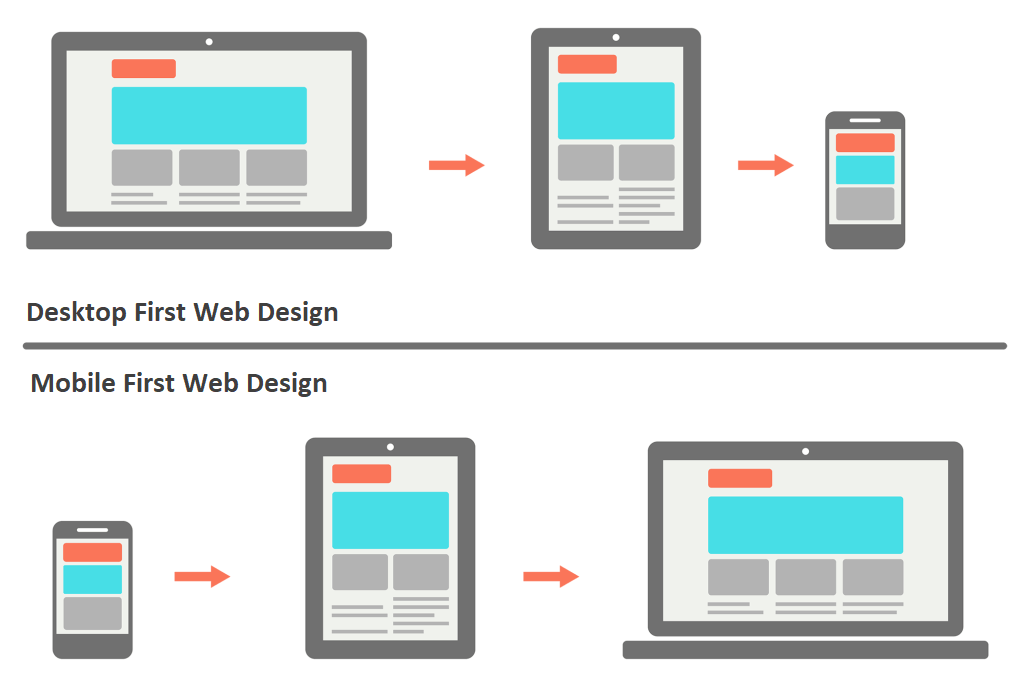
\includegraphics[width=1.0\textwidth]{DesktopMobileFirst}
\caption[Desktop-First und Mobile-First]{Desktop-First und Mobile-First\\ Quelle: \url{http://fredericgonzalo.com/en/2017/03/01/understanding-the-difference-between-mobile-first-adaptive-and-responsive-design/}}\label{fig:DesktopMobileFirst}
\end{figure}

\subsection{Bootstrap} \label{Bootstrap}
Aufgrund der Unterstützung für die Informatik Studierenden (\hyperlink{/LE10/}{/LE10/}und \hyperlink{/LE40/}{/LE40/}), die den Laptop fast täglich verwenden müssen, den Wartungsaufwand und die Implementierungskomplexität, wird eine Responsive-Website mit ``Laptop-First'' Strategie (Bildschirmgröße $\geq$ 768 px) gewählt. Um eine Responsive-Website schneller und einfacher gestalten zu können, wird Bootstrap verwendet.

Bootstrap ist ein beliebtes, kostenloses HTML-, CSS- und JavaScript-Framework zum Entwickeln von Responsive-Websites mit Priorisierung von Mobilgeräten. Das Framework enthält Responsive-CSS- und -HTML-Vorlagen für Schaltflächen, Tabellen, Navigation, Bildkarussells und andere Elemente, die man auf der Webseite verwenden kann. Es sind einige optionale JavaScript-Plugins verfügbar, die selbst Entwicklern mit lediglich grundlegenden Codierungskenntnissen das Entwickeln großartiger Responsive-Websites ermöglichen. Bootstrap ist mit allen modernen Browsern kompatibel wie (\hyperlink{/LE10/}{Chrome}), Firefox, Internet Explorer, Safari und Opera \cite{bootstrapworld}.

\begin{figure}[ !h] \centering
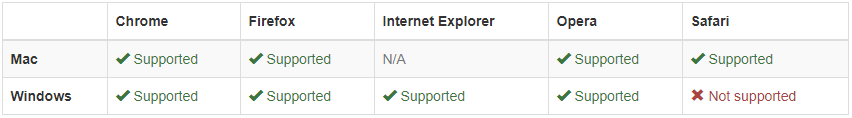
\includegraphics[width=1.0\textwidth]{DesktopBrowsers}
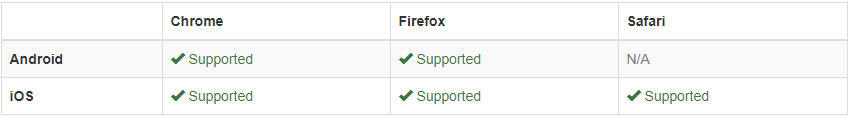
\includegraphics[width=1.0\textwidth]{MobileBrowsers}
\caption[Unterstützte Browsers von Bootstrap]{Unterstützte Browsers von Bootstrap\\ Quelle: \url{https://getbootstrap.com/docs/3.3/getting-started/\# support}}\label{fig:DesktopMobileBrowsers}
\end{figure}

Bootstrap wurde 2010 von Twitter unter dem Namen „Twitter Bootstrap“ entwickelt, mit dem Ziel eine einheitliche Bibliothek für die Gestaltung von Weboberflächen zu schaffen. Das Problem war damals, dass für die Designentwicklung bei Twitter viele verschiedene Bibliotheken verwendet wurden. Das führte zu Inkonsistenzen und einem großen Wartungsaufwand. Bootstrap sollte eine gemeinsame Basis schaffen, mit der alle Mitarbeiter arbeiten konnten, um schnell und einfach Websites zu gestalten.
Im August 2011 entschloss sich Twitter dazu, das Bootstrap Framework als Open Source Projekt zu veröffentlichen. Damit war der Siegeszug dieses ausgezeichneten und leicht zu bedienenden Frontend-Frameworks zur Webdesign-Gestaltung nicht mehr aufzuhalten\cite{bootstrap}.

Um Bootstrap zu verwenden, muss man HTML und CSS nicht gut kennen. Es ist ein Vorteil, wenn man ein Backend-Entwickler ist und einige UI-Änderungen vornehmen kann. 
%Bootstrap ist vollständig anpassbar, man kann wählen, welche Komponenten man verwenden möchte und verwendet eine Variablen-Datei, um noch mehr Farbe und Verhalten zum Anpassung zu bekommen. Alles, was man tun muss, ist es die Seite \url{http://getbootstrap.com/customize/} zu besuchen. Dann wählt man die benötigten Plugins aus und klickt man auf Downloaden. 
%Bootstrap bietet auch eine Möglichkeit, die internen Variablen für fortgeschrittene Benutzer zu überschreiben, aber sie bieten ziemlich ordentliche Standardwerte, so dass man sich darüber keine Gedanken machen sollte, es sei denn, man muss dies tun.

%Bootstrap bietet viele Hilfsklassen, die die Entwicklung einer responsiven Website einfach und schnell machen. Man kann jedes Layout mit fester Breite in ein flüssiges Layout umwandeln, indem man einfach seine übergeordnete \textit{.container} Klasse in \textit{.container-fluid} ändern. Bootstrap verfügt außerdem über die Klassen \textit{.visible}, mit denen man steuern kann, wie seine Section auf Tablets und mobilen Geräten angezeigt werden. Beispiel:
%
%\textit{<div class = ``sichtbarer-xs-block visible-sm-block''> </ div>}
%
%In diesem Fall wird das div als ein Section mit display angezeigt: block nur auf Telefonen und Tablets. Es wird auf dem Desktop versteckt werden.

%Um Bootstrap in einer HTML-Seite zu verwenden, muss lediglich ein fertiges ZIP-Archiv von der Bootstrap-Webseite \url{http://getbootstrap.com/docs/3.3/getting-started/\# download} heruntergeladen werden. 
Bootstrap-Bibliothek kann als ein ZIP-Archiv von der Bootstrap-Webseite \url{http://getbootstrap.com/docs/3.3/getting-started/\# download} heruntergeladen werden. Dieses Archiv enthält bereits fast alle benötigten, in das eigene Projekt einzubindenden Dateien, wie eine Stylesheetdatei mit allen Komponenten, eine JavaScript-Datei mit allen Plugins und auch eine benötigte Icon-Schriftart. Alternativ gibt es auf GitHub noch ein vollständiges, deutlich umfangreicheres ZIP-Archiv für Entwickler herunterzuladen, welches auch Beispiele für typische Webseiten zur bequemen Verwendung als Ausgangsdatei und vieles weitere enthält.

Die Dateien im ZIP-Archiv müssen in das eigene HTML-Dokument/Projekt eingebunden werden. Soll auch mit JavaScript-Komponenten gearbeitet werden, so muss die JavaScript-Datei zusammen mit der jQuery-Bibliothek ebenfalls im HTML-Dokument referenziert werden. Möchte man angepasste Einstellungen für Stil und JavaScript-Funktionalität, besteht die Möglichkeit, fast alle Elemente von Bootstrap auf der Website selbst zu verändern und ein angepasstes Paket herunterzuladen. Schließlich kann man Bootstrap auch lokal, seinen Bedürfnissen entsprechend, vom Standard abweichend kompilieren.

Das folgende Beispiel verdeutlicht die Funktionsweise. Der HTML-Quellcode definiert ein einfaches Suchformular sowie eine Ergebnisliste in Form einer Tabelle. Die Seite besteht aus regulären, semantisch verwendeten HTML5-Elementen sowie einigen zusätzlichen CSS-Klassenangaben entsprechend der Bootstrap-Dokumentation \cite{bootstrapwiki}.

\lstinputlisting[language=HTML, caption=Bootstrap Beispiel, basicstyle=\scriptsize]{ex.html}
%\begin{lstlisting}[language=HTML, caption=Bootstrap Beispiel]
%<!DOCTYPE html>
%<html>
%
%  <head>
%    <title>Bootstrap Beispiel</title>
%
%    <!-- Einbinden des Bootstrap-Stylesheets -->
%    <link rel="stylesheet" href="https://ajax.aspnetcdn.com/ajax/bootstrap/3.3.7/css/bootstrap.min.css">
%
%    <!-- optional: Einbinden der jQuery-Bibliothek -->
%    <script src="https://ajax.aspnetcdn.com/ajax/jQuery/jquery-1.12.4.min.js"></script>
%
%    <!-- optional: Einbinden der Bootstrap-JavaScript-Plugins -->
%    <script src="https://ajax.aspnetcdn.com/ajax/bootstrap/3.3.7/bootstrap.min.js"></script>
%  </head>
%
%  <body>
%    <section class="container">
%      <h1>Suche</h1>
%      <p>Beispiel für ein einfaches Suchformular.</p>
%      <!-- Suchformular mit Eingabefeld und Button -->
%      <form class="well form-search">
%        <input type="text" class="input-medium search-query"/>
%        <button type="submit" class="btn btn-primary">Search</button>
%      </form>
%
%      <h2>Ergebnisse</h2>
%      <!-- Tabelle mit abwechselnder Zellenhintergrundfarbe und Ausserrahmen -->
%      <table class="table table-striped table-bordered">
%     
%      </table>
%    </section>
%  </body>
%
%</html>
%\end{lstlisting}

\textbf{Grid System}

Das Grid-System ist eines der wichtigsten Konzepte in Bootstrap, das beschreibt, wie man Komponenten auf der Oberfläche positionieren und wie man eine Responsive-Website implementieren kann. Im Grid-System ist das Layout der Seite in verschiedene Zeilen aufgeteilt. Jede Zeile hat maximal 12 Spalten (möglicherweise weniger). Basierend auf der Breite des Anzeigegerätetyps kann man verschiedene CSS-Klassen verwenden, um die Anzahl der Anzeigespalten anzupassen. Zum Beispiel hat man eine Webseite, die das Grid Layout System wie folgt verwendet:  

\begin{figure}[ !h] \centering
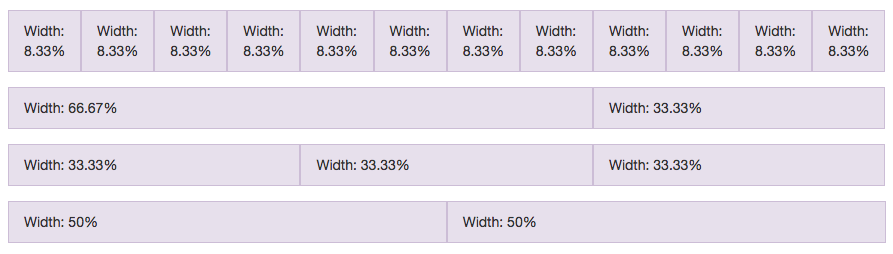
\includegraphics[width=1.0\textwidth]{BootstrapGridSystem}
\caption[Beispiel Grid System]{Beispiel Grid System}\label{fig:BootstrapGridSystem}
\end{figure}

Die Abbildung \ref{fig:BootstrapGridSystem} hat vier verschiedene Zeilen, wobei jede Zeile eine andere Anzahl von Spalten hat, beispielsweise die erste Zeile hat 12 Spalten. Die CSS-Klasse, die auf die Spalte angewendet wird, ist in fünf verschiedene Kategorien unterteilt (Tabelle \ref{tab:BootstrapGridSystem}). 

\begin{table}[h]
\footnotesize
	\begin{center}
			\begin{tabular}{|l|c|c|c|c|c|}
			\hline
			&\textbf{Extra klein}&\textbf{Klein}&\textbf{Medium}&\textbf{Groß}&\textbf{Extragroß}\\
			& <576px & $\geq$ 576px & $\geq$ 768px&$\geq$ 992px &$\geq$ 1200px\\
			\hline
			\textbf{Maximale }&Keine&540px&120px&960px&1140px\\
			\textbf{Behäterbreite}&(automatisch)&&&&\\
			\hline
			\textbf{Klassenpräfix}&.col-&.col-sm-&.col-md-&.col-lg-&.col-xl-\\
			\hline
			\textbf{Anzahl der Spalten}&\multicolumn{5}{|c|}{12}\\
			\hline
			\textbf{Stegbreite}&\multicolumn{5}{|c|}{30px(15px auf jeder Seite einer Spalte)}\\
			\hline
			\textbf{Nestbar}&\multicolumn{5}{|c|}{Ja}\\
			\hline
			\textbf{Spaltenbestellung}&\multicolumn{5}{|c|}{Ja}\\
			\hline
			\end{tabular}
	\end{center}
	\caption[Rasteroptionen im Bootstrap-Framework]{Rasteroptionen\\Quelle: https://getbootstrap.com/docs/4.1/layout/grid/}
	\label{tab:BootstrapGridSystem}
\end{table}		

Wenn es nur 1 Block \textit{<div class=``col-md''> </div>} und keine Spaltennummer gibt, ist der Standardwert 12 Spalten (voller Block von Containern). Wenn man 3 Blöcke \textit{<div class=``col-md''> </div>} hat, werden die Blöcke automatisch ebenso wie \textit{<div class=``col-md-4''> </div>} unterteilt. Die Bildschirme, die größer als den verwendeten Bildschirm sind, ändern sich nicht. Die kleineren Bildschirme werden automatisch auf \textit{col-12} (eine Spalte pro Zeile) umgeschaltet, wenn keine andere Anpassung vorgenommen wird. Das folgende Beispiel verdeutlicht die Funktionsweise des Grid System.

Zuerst fügt man dieses Meta-Tag dem Head-Tag hinzu.
\begin{lstlisting}[language=HTML, basicstyle=\scriptsize]
<meta name="viewport" content="width=device-width, initial-scale=1.0">
\end{lstlisting}	
Und das Body-Tag ist wie folgt:
\begin{lstlisting}[language=HTML, caption= Beispiel Grid System,basicstyle=\scriptsize]
<div class="container" style="background-color: grey; margin-bottom: 50px;">
   <div class="row">
      <div class="col-md-4 col-sm-6">
         <div class="block"></div>
      </div>
      <div class="col-md-8 col-sm-6">
         <div class="block"></div>
      </div>
   </div>
</div>
\end{lstlisting}
Ergebnisse des Laufs des obigen Codes:
\begin{itemize}
\item Wenn die Bildschirmbreite größer als 768px ist, wird jede Zeile in zwei Spalten aufgeteilt: Eine Spalte belegt 33,33 \% der Bildschirmbreite und eine Spalte belegt 66,67 \% der Bildschirmbreite.
\item  Wenn die Bildschirmbreite weniger als 768px ist, wird jede Zeile in zwei Spalten aufgeteilt: Jede Spalte belegt 50\% der Bildschirmbreite.
\item Wenn die Bildschirmbreite weniger als 576px ist, hat jede Zeile nur eine Spalte.
\end{itemize}

Die Dokumentation von Bootstrap ist essentiell. Bootstrap hat eine umfangreiche Dokumentation inklusive Demos, die auch für Anfänger in dem Bereich leicht nachvollziehbar sind und bis hin zu den komplexesten Elementen alles für den Nutzer zugänglich macht. Unter \url{http://getbootstrap.com/getting-started/\# template} kann man eine grundlegende Vorlage und eine Reihe von Beispielen für unterschiedliche Bedürfnisse \url{http://getbootstrap.com/getting-started/\# examples} herunterladen. Man kann einfach das Bootstrap-Repository herunterladen, in den Ordner \textit{docs / examples} gehen, das gewünschte Beispiel kopieren / einfügen und daran arbeiten.
%https://www.htmlgoodies.com/html5/markup/10-common-uses-of-bootstrap.html


%1. Zunächst ist Bootstrap das beliebteste Framework zum Erstellen von Layouts. Hier sind einige zusätzliche Gründe Bootstrap zu verwenden:
%
%Das reaktionsschnelle CSS von Bootstrap passt sich an Telefone, Tablets und Desktops an
%Mobile-First-Styles sind Teil des Frameworks
%Bootstrap ist mit allen modernen Browsern kompatibel (Chrome, Firefox, Internet Explorer, Safari und Opera).
%2. Bootstrap hat eine große Community und freundlichen Support. Für Ressourcen besuchen Sie:
%Schau dir den Bootstrap Blog an.
%Sie können mit Bootstrappern mit IRC im irc.freenode.net Server im ## bootstrap channel chatten.
%Schaut euch an, was die Leute mit Bootstrap auf der Bootstrap Expo machen.
%3. Bootstrap ist einfach einzurichten und ein funktionierendes Layout in weniger als einer Stunde zu erstellen
%
%Sie haben eine grundlegende Vorlage unter http://getbootstrap.com/getting-started/#template und eine Reihe von Beispielen für unterschiedliche Bedürfnisse (http://getbootstrap.com/getting-started/#examples). Sie können einfach das Bootstrap-Repository herunterladen, in den Ordner docs / examples gehen, das gewünschte Beispiel kopieren / einfügen und daran arbeiten.
%
%4. Sie müssen HTML und CSS nicht gut kennen, um Bootstrap zu verwenden, es ist ein Vorteil, wenn Sie ein Backend-Entwickler sind und einige UI-Änderungen vornehmen müssen.
%
%5. Es ist vollständig anpassbar, ich kann wählen, welche Komponenten ich verwenden möchte und verwenden Sie Variablen-Datei, um noch mehr Farbe und Verhalten Anpassung zu bekommen.
%
%Alles, was Sie tun müssen, ist http://getbootstrap.com/customize/, wählen Sie die benötigten Plugins aus und klicken Sie auf Download. Bootstrap bietet auch eine Möglichkeit, die internen Variablen für fortgeschrittene Benutzer zu überschreiben, aber sie bieten ziemlich ordentliche Standardwerte, so dass Sie sich darüber keine Gedanken machen sollten, es sei denn, Sie müssen dies tun.
%
%6. Wenn Sie die Bootstrap-Version aktualisieren, werden Sie nicht viele Fehler sehen, da sich das Kernteam um die Abwärtskompatibilität kümmert.
%
%7. Ihre Dokumentation ist großartig! Hier sind einige Ressourcen zum Auschecken:
%
%Bootstrap 3 Tutorial
%Code Academy: Bootstrap
%Webdesign-Tutorials: Bootstrap
%8. Bootstrap bietet viele Hilfsklassen, die die Entwicklung einer responsiven Website einfach und schnell machen.
%
%Sie können jedes Layout mit fester Breite in ein flüssiges Layout umwandeln, indem Sie einfach Ihre übergeordnete .container-Klasse in .container-fluid ändern.
%
%Bootstrap verfügt außerdem über die Klassen .visible - * - *, mit denen Sie steuern können, wie Ihre Abschnitte auf Tablets und mobilen Geräten angezeigt werden. Beispiel:
%
%<div class = "sichtbarer-xs-block visible-sm-block"> </ div>
%
%In diesem Fall wird das div als ein Abschnitt mit display angezeigt: block nur auf Telefonen und Tablets. Es wird auf dem Desktop versteckt werden.
%
%9. Bootstrap-Komponenten sind gut in das Ökosystem der beliebten JS MVC Frameworks wie Angular übernommen. Bootstrap bietet mehrere Möglichkeiten, es in Ihr Projekt einzubinden:
%
%Benutzung der Laube:
%
%Bower installieren Bootstrap
%
%Verwenden von npm:
%
%npm install bootstrap
%
%Und einfach ein Skript-Tag mit der URL hinzufügen, um Source auf CDN zu laden.
%
%Wir haben auch ui-bootstrap für Angular.js und react-bootstrap für React. Sie können sie auch über Bower und Npm installieren. Um zum Beispiel ein Kollaps-Element zu erstellen, müssen Sie nur ein ähnliches Markup erstellen:
%
%<div uib-collapse = "isCollapsed">
%
%<div class = "well well-lg">
%
%Inhalt des Einsturzes
%
%</ div>
%
%</ div>
%
%Anstatt eine Menge jQuery-Konfiguration zu machen, wie Sie es normalerweise tun würden.
%
%10. Bootstrap löst viele browserübergreifende Probleme auf und Sie müssen sich nicht ständig darum kümmern.
%
%Hinweis: Bootstrap wurde für die Verwendung mit den neuesten Desktop- und mobilen Browsern entwickelt. Dies bedeutet, dass die Anzeigen in älteren Browsern möglicherweise anders aussehen und möglicherweise anders gerendert werden, obwohl die Anzeigen gemäß der Dokumentation voll funktionsfähig sein sollten.
%
%Hier sind ein paar Screenshots zur Browserkompatibilität.







%Note
%https://www.nngroup.com/articles/mobile-vs-responsive/
%\url{https://www.clickseed.com/responsive-design-vs-separate-mobile-site-vs-dynamic-serving/}
%\url{https://www.interaction-design.org/literature/article/adaptive-vs-responsive-design}
	\section{Google chart tools}
Um den Tableau zu visualisieren, braucht man ein Werkzeug, das einfach zu bedienen und kostenlos ist. Mit dieser Anforderungen ist Google Charts ein guter Kandidat.

%https://reviews.financesonline.com/p/google-chart-tools/
Google chart tools \cite{googleCharts}(Google Charts, unterscheidet sich von dem Google Chart API) ist ein interaktiver Webservice \cite{googleChartswiki}, mit dem Benutzer ihre Daten auf ihrer Website über einfache oder attraktive Visualisierungen anzeigen können. Das Werkzeug wird häufig mit einem einfachen JavaScript verwendet, das auf der Webseite eingebettet ist. Mit Google Charts können Benutzer die einfachen Diagramme wie Liniendiagramme bis hin zu komplexen Diagrammen wie Baumdiagramme, erstellen. 

Neben dem standardmäßigen Google-Design werden den Nutzern auch zahlreiche Anpassungsoptionen für ihre Diagramme zur Verfügung gestellt. Das Werkzeug ist recht einfach zu bedienen, da Benutzer nur die Anwendung einbetten, die Google Chart-Bibliotheken laden und die zu charternden Daten eingeben müssen. Nach ein paar Anpassungen und der Zuweisung einer ID kann das Diagramm auf der Webseite aktiviert werden.

Google Charts ist nicht nur kostenlos, sondern auch eine benutzerfreundliche Anwendung. Mit ein wenig JavaScript-Kenntnissen kann man komplizierteste Diagramme und Grafiken erstellen. Die Anpassungsoptionen sind auch ein weiterer erwähnenswerter Vorteil. Diagramme können mit Farben, Linien, Überlagerungen, Punkten usw. angepasst und optimiert werden, damit sie sich leicht an die Schnittstelle der Webseite anpassen. Es gibt eine großartige Dokumentation von Google, die  unter der Seite \url{https://developers.google.com/chart/interactive/docs/} nachgeschlagen werden kann.

%https://www.moesif.com/blog/technical/visualization/How-to-Choose-the-Best-Javascript-Data-Visualization-Library/
Gegen die Verwendung von Google Charts spricht zum einen, dass eine Netzwerkverbindung erforderlich ist. Außerdem ist es durch Google den Benutzern nicht gestattet, den Code selbst zu speichern oder zu hosten. Diese Einschränkungen haben jedoch keinen Einfluss auf die Anforderungen der Tableau-Anwendung.
%Und obwohl Google Charts zwar kostenlos ist, ist es aber keine Open Source-Version, es gelten die Google API-Nutzungsbedingungen. 

\subsection{Organigramm}\label{Organigramm}
Da die Struktur von Tableau ein Baum ist, eignet sich das Organigramm von Google Charts gut zur Visualisierung eines Tableaus.

Organigramme sind ein Diagramm einer Knotenhierarchie, die häufig verwendet wird, um übergeordnete / untergeordnete Beziehungen in einer Organisation darzustellen. Eine Baumfamilie ist eine Art Organigramm\cite{orgCharts}.
Der folgenden HTML-Quellcode definiert ein einfaches Organigramme \cite{orgCharts}.

\lstinputlisting[language=JavaScript, caption=Organigramme Beispiel,basicstyle=\scriptsize]{googlecharts_organization_chart.htm}

Zuerst muss man den Loader selbst laden, was in einem separaten \textit{script}-Tag mit erfolgt: 
\begin{lstlisting}[language=HTML,basicstyle=\scriptsize]
	src="https://www.gstatic.com/charts/loader.js"
\end{lstlisting} 
Dieses Tag kann sich entweder im ``head'' oder ``body'' des Dokuments befinden oder dynamisch in das Dokument eingefügt werden. %, während es geladen wird oder nachdem das Laden abgeschlossen wurde.\\
Nachdem der Loader geladen wurde, kann man \textit{google.charts.load} abrufen. 
%Wo man es aufruft, kann es sich in einem script Tag im head oder body des Dokuments befinden, und man kann es aufrufen, während das Dokument noch geladen wird oder zu einem beliebigen Zeitpunkt nach dem Laden.\\
Ab Version 45 kann man \textit{google.charts.load} mehr als einmal abrufen, um weitere Pakete zu laden, aber wenn man dies tut, muss man jedes Mal dieselbe Versionsnummer und dieselbe Spracheinstellung angeben.\\

\begin{lstlisting}[language=JavaScript,basicstyle=\scriptsize]
google.charts.load('current', {packages:"orgchar"]});
\end{lstlisting}

Das erste Argument des \textit{google.charts.load} ist der Name oder die Nummer der Version als String. 
%Zu diesem Zeitpunkt gibt es nur zwei spezielle Versionsnamen und mehrere eingefrorene Versionen.
Wenn man  \textit{current} angibt, wird dadurch die neueste offizielle Version von Google Charts geladen. 
%Wenn man den Kandidaten für das nächste Release testen möchten, verwenden Sie 'upcoming'stattdessen.
Der zweite Parameter des \textit{google.charts.load} ist ein Objekt zum Festlegen von Einstellungen wie Pakete, Sprache, Rückrufen... In dem obigen Beispiel ist \textit{orgchar} der Paketname.

Bevor man eines der von \textit{google.charts.load} geladenen Pakete verwenden kann, muss man warten, bis das Laden beendet ist. 
%Es reicht nicht aus, nur auf das Laden des Dokuments zu warten.
Da es einige Zeit dauern kann, bis das Laden beendet ist, muss man eine Rückruffunktion registrieren. Es gibt zwei Möglichkeiten, dies zu tun. Man gibt entweder eine callback Einstellung in dem \textit{google.charts.load} an oder ruft \textit{setOnLoadCallback} mit einer Funktion (z.B \textit{drawChart()}) als Argument auf.


%Beachtet man, dass man eine Funktionsdefinition bereitstellen muss, anstatt die Funktion aufzurufen. Die angegebene Funktion kann entweder eine benannte Funktion oder eine anonyme Funktion sein. Wenn die Pakete geladen sind, wird diese Callback-Funktion ohne Argumente aufgerufen. Das Ladeprogramm wartet auch auf das Laden des Dokuments, bevor es den Rückruf aufruft.
%
%\begin{lstlisting}[language=HTML, caption=Bootstrap Beispiel]
%google.charts.setOnLoadCallback ( ZeichenChart1 ); 
%  google.charts.setOnLoadCallback ( ZeichenChart2 ); 
%  // ODER 
%  google.charts.setOnLoadCallback ( 
%    function () {// Anonyme Funktion, die drawChart1 und drawChart2 
%         aufruft drawChart1 (); 
%         drawChart2 (); 
%      } );
%\end{lstlisting}


%Wenn man mehr als ein Diagramm zeichnen möchte, kann man entweder mehrere Callback-Funktionen registrieren oder diese zu einer Funktion zusammenfassen.
 
%Wenn man mehrere Diagramme auf einer Webseite zeichnen möchte, fügt man folgenden Code auf \textit{<head>} der Seite hinzu:
%\begin{itemize}
%\item	Ladet man alle von den Diagrammen benötigten Pakete in einem einzigen Aufruf nach \textit{google.charts.load()}.
%\item	Für jede Tabelle auf der Seite, fügt man einen Anruf \textit{google.charts.setOnLoadCallback()} mit dem Rückruf, der das Diagramm als Eingabe zeichnet.
%\end{itemize}
%Wenn man mehrere Diagramme für die gleichen Daten zeichnen möchte, ist es möglicherweise einfacher, einen einzelnen Rückruf für beide Diagramme zu schreiben.

%Vorbereiten die Daten
\subsection{DataTable}
Alle Diagramme benötigen Daten. Google Chart Tools-Diagramme erfordern das Umbrechen von Daten in eine JavaScript-Klasse namens \textit{google.} \textit{visualization.DataTable}. Diese Klasse ist in der Google Visualization-Bibliothek definiert, die man zuvor geladen hat.

Die Organigramm erfordert eine \textit{DataTable} mit drei Spalten, wobei jede Zeile einen Knoten im Organigramm darstellt. Hier sind die drei Spalten:
\begin{itemize}
\item	Spalte 0 : Die Knoten-ID. Es sollte unter allen Knoten \textit{eindeutig} sein und beliebige Zeichen einschließlich Leerzeichen enthalten. Dies wird auf dem Knoten angezeigt. Man kann einen formatierten Wert angeben, der stattdessen im Diagramm angezeigt wird. Der unformatierte Wert wird jedoch weiterhin als ID verwendet.
\item 	Spalte 1(optional): Die ID des übergeordneten Knotens. 
\item	Spalte 2(optional): Tooltip-Text, der angezeigt wird, wenn ein Benutzer den Mauszeiger über diesen Knoten bewegt.
\end{itemize}
Jeder Knoten kann keinen oder einen übergeordneten Knoten und keinen oder mehrere untergeordnete Knoten haben.

\subsection{Zeichnen des Diagramms}
Der letzte Schritt ist das Zeichnen des Diagramms. Zuerst muss man eine Instanz der Diagrammklasse, die man verwenden möchte, instanziieren und dann muss man \textit{draw()} aufrufen.
Jeder Diagrammtyp basiert auf einer anderen Klasse, die in der Diagrammdokumentation aufgeführt ist, z.B. basiert das Organigramm auf der \textit{google.visualization.OrgChart}. 

\begin{lstlisting}[language=JavaScript,basicstyle=\scriptsize]
var chart = new google.visualization.OrgChart(document.getElementById('chart_div'));
\end{lstlisting}

Nachdem man seine Daten und Optionen vorbereitet hat, kann man das Diagramm zeichnen. Die Seite muss ein HTML-Element (normalerweise ein \textit{<div>}) enthalten, um das Diagramm zu halten. Man muss dem Diagramm einen Verweis auf dieses Element übergeben, also weist man ihm eine ID zu, mit der man einen Verweis \textit{document.getElementById()} abrufen kann. Alles in diesem Element wird beim Zeichnen durch das Diagramm ersetzt. 

Jedes Diagramm unterstützt eine \textit{draw()} \textit{Methode} \cite{drawCharts}, die zwei Werte akzeptiert: ein \textit{DataTable} (oder ein \textit{DataView}) Objekt, das seine Daten enthält, und ein optionales Diagrammoptionsobjekt. Das Optionsobjekt ist nicht erforderlich, und man kann es ignorieren oder \textit{Null} übergeben, um die Standardoptionen des Diagramms zu verwenden.

Nach dem Aufruf \textit{draw()} wird das Diagramm auf der Seite gezeichnet. Man soll die \textit{draw()} Methode jedes Mal aufrufen, wenn man die Daten oder die Optionen ändern und das Diagramm aktualisieren möchte. Die \textit{draw()} Methode ist asynchron, d.h. sie wird sofort zurückgegeben während die zurückgegebene Instanz jedoch möglicherweise nicht sofort verfügbar ist.

%Die \textit{draw()} Methode ist asynchron, dh sie wird sofort zurückgegeben während die zurückgegebene Instanz jedoch möglicherweise nicht sofort verfügbar ist. In vielen Fällen ist das in Ordnung, das Diagramm wird schließlich gezeichnet. Wenn man jedoch Werte in einem Diagramm nach dem Aufruf festlegen oder abrufen möchten \textit{draw()}, muss man darauf warten, dass das Ereignis  ``ready'' ausgelöst wird, wodurch angezeigt wird, dass es ausgefüllt ist. 

Außerdem gibt es noch viele Einstellungsmöglichkeiten wie Farbe oder Größe der Diagramme sowie die Methoden und Events..., die unter der Seite \url{https://developers.google.com/chart/interactive/docs/gallery/orgchart} nachgeschlagen werden.  



	\section{Jasmine}
Um schon während der Entwicklung eine gute Qualität des Quelltextes anzustreben, ist der Einsatz von einem Testing-Framework sinnvoll. Die Wahl fällt auf Jasmine, da es eine einfache Implementierung ermöglicht sowie clientseitig ohne einen Server funktioniert. 

Jasmine ist ein verhaltensorientiertes Entwicklungsframework zum Testen von JavaScript-Code. Es hängt nicht von anderen JavaScript-Frameworks ab. Es benötigt kein DOM. Und es hat eine saubere, explizite Syntax, so dass man problemlos Tests schreiben kann \cite{jasmine}. Zusätzlich folgt Jasmine der BDD-Prozedur (Behavior Driven Development), um sicherzustellen, dass jede Zeile der JavaScript-Anweisung ordnungsgemäß Unit-getestet ist. Durch das Befolgen der BDD-Prozedur bietet Jasmine eine kleine Syntax, um die kleinste Einheit der gesamten Anwendung zu testen, anstatt sie als Ganzes zu testen.  

Im Folgenden sind die Vorteile der Verwendung von Jasmine gegenüber anderen verfügbaren JavaScript-Test-Frameworks aufgeführt \cite{jasmineTutorial}.
\begin{itemize}
\item	Jasmine ist von keinem anderen JavaScript-Framework abhängig.
\item	Jasmine benötigt kein DOM.
\item	Die gesamte im Jasmine-Framework verwendete Syntax ist sauber und offensichtlich.
\item	Jasmine wird stark von Rspec, JS Spec und Jspec beeinflusst.
\item	Jasmine ist ein Open-Source-Framework und leicht verfügbar in verschiedenen Versionen wie Stand-alone, Ruby-Juwel, Node.js, etc.
\end{itemize}



\subsection{Wie benutzt man Jasmin?}
%Man kann Jasmine unter \url{https://github.com/jasmine/jasmine/releases} herunterladen.
Jasmine ist sehr einfach in jeder Art von Entwicklungsmethodik zu implementieren. Alles, was man herunterladen muss, ist die Standalone-Bibliotheksdateien von der offiziellen Website \url{https://github.com/jasmine/jasmine/releases}. Dieses implementiert man gleich in seiner Anwendung. Nach dem Entpacken der Jasmine-Bibliothek muss man den Entpacker-Ordner in den Unit-Tests-Ordner der erstellten Anwendung einfügen. Der Entpacker-Ordner umfasst:
\begin{figure}[ !h] \centering
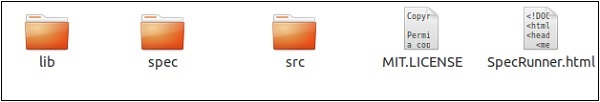
\includegraphics[width=1.0\textwidth]{jasmineLib}
\caption[Jasmine-Bibliotheksdateien]{Jasmine Standalone-Bibliotheksdateien\\ Quelle: \url{https://www.tutorialspoint.com/jasminejs/jasminejs_overview.htm}}\label{fig:jasmineLib}
\end{figure}
\begin{itemize}
\item	\textit{Lib:} enthält Quellcode für das Framework.
\item	\textit{Spec}: enthält Code für seine Tests
\item	\textit{Src:} enthält Quellcode für seine Anwendung
\item 	\textit{SpecRunner.html:} ist eine Seite, die man Tests ausführt.
%Man können Verweise auf seine Spezifikationen (Tests) und den Quellcode für die Anwendung sehen, die Sie testen möchten. Es ist also nicht notwendig, den Code in den Ordner \textit{``src''} zu kopieren. Man kann einfach Ihre Spezifikationen in diese Datei einbinden.
\end{itemize}
Dieses Paket enthält auch ein kleines Beispiel, das nützlich sein könnte.

\subsection{Wie man mit Jasmine JS Tests prüft?}
Ein einfaches Beispiel für JavaScript-Tests von Jasmine sieht folgendermaßen aus:
%https://www.apriorit.com/dev-blog/372-testing-javascript-with-jasmine
\begin{lstlisting}[language=JavaScript,basicstyle=\scriptsize]
describe("App", function () {
    describe("foo", function () {
        it("should return bar", function () {
            expect(App.foo()).toEqual("bar");
        });
    });
});

var App = {
    foo: function() {
        return "bar123";
    }
};
\end{lstlisting}

Im obigen Beispiel wird \textit{App.foo(}) durch die Suite \textit{``App''} mit Matcher \textit{.toEqual} getestet. 

%https://www.htmlgoodies.com/beyond/javascript/testing-javascript-using-the-jasmine-framework.html
Eine Suite stellt eine Reihe von verwandten Tests dar. Jede Suite enthält wiederum eine Reihe von Erwartungen, die die Ergebnisse des Tests - den tatsächlichen Wert - mit dem erwarteten Wert vergleichen. Eine Suite wird durch Aufrufen der Funktion \textit{describe()} definiert. Es benötigt zwei Parameter: den Namen der Suite und die Funktion, die die Aufrufe der Erwartungs-Methoden enthält. Diese werden mit der Methode \textit{it()} definiert. Wie \textit{describe()} akzeptiert \textit{it()} auch einen Namen und einen Funktionsparameter. Der Funktionsparameter \textit{it()} kann Variablen und einen oder mehrere Aufrufe der \textit{expect()} enthalten. In Verbindung mit einer Matcher-Funktion führen diese die Aufgabe durch, die Ist- und Erwartungswerte zu vergleichen. Jeder Matcher implementiert einen booleschen Vergleich zwischen dem tatsächlichen Wert und dem erwarteten Wert. Es ist verantwortlich für die Berichterstattung an Jasmine, wenn die Erwartung wahr oder falsch ist. Jasmine wird dann die Spezifikation bestehen oder nicht bestehen.

Jeder Matcher kann eine negative Assertion auswerten, indem er den Call \textit{expect()} mit einem \textit{``not''} vor dem Aufruf des Matcher verkettet. Jasmine bietet eine große Auswahl an Matching-Tools. Die vollständige Liste findet man auf der Seite \url{https://jasmine.github.io/api/edge/matchers.html}.

Um einer Test-Suite zu helfen, doppelten Konfigurations- und Teardown-Code zu löschen, stellt Jasmine die globalen Funktionen \textit{beforeEach}, \textit{afterEach},\textit{ beforeAll} und \textit{afterAll} bereit. 
Wie der Name schon sagt, wird die \textit{beforeEach} Funktion einmal vor jeder Spezifikation in der \textit{describe} aufgerufen, in der sie aufgerufen wird und die \textit{afterEach} Funktion wird einmal nach jeder Spezifikation aufgerufen. Die \textit{beforeAll} Funktion wird nur einmal aufgerufen, bevor alle Spezifikationen \textit{describe} ausgeführt werden und die \textit{afterAll} Funktion wird nach Abschluss aller Spezifikationen aufgerufen \textit{beforeAll} und\textit{ afterAll} kann verwendet werden, um Testsuiten mit teurem Setup und Teardown zu beschleunigen.

%Seien Sie jedoch vorsichtig mit beforeAll und afterAll! Da sie nicht zwischen den Spezifikationen zurückgesetzt werden, ist es leicht, den Status zwischen Ihren Spezifikationen versehentlich zu verlieren, so dass sie fälschlicherweise bestehen oder fehlschlagen.

%https://www.apriorit.com/dev-blog/372-testing-javascript-with-jasmine
%Setup- und Teardown-Code sollte in den globalen beforeEach () - und afterEach () -Methoden platziert werden. Diese sind nützlich, um Testwerte zwischen Tests neu zu initialisieren und zu setzen. Die beforeEach () -Methode wird vor jeder spec (it () -Methode im describe aufgerufen und afterEach () wird nach jeder Spezifikation aufgerufen.

\begin{lstlisting}[language=JavaScript,basicstyle=\scriptsize]
describe ( "A suite with some common settings" ,  function(){ 
  var  foo  =  0 ;
  beforeEach ( Funktion(){ 
    foo  + =  1 ; 
  });  
  afterEach ( Funktion(){ 
    foo  =  0 ; 
  });  
  beforeAll ( Funktion(){ 
    foo  =  1 ; 
  });  
  afterAll ( Funktion(){ 
    foo  =  0 ; 
  });  
});
\end{lstlisting}

Die Ausführliche Anleitung zur Jasmine-Framework kann man auf der Seite \url{https://jasmine.github.io/pages/docs_home.html} lesen. 

%\cleardoublepage		
\chapter{Architektur}\label{sec:Architektur}
Dieses Kapitel handelt von der Umsetzung der Anforderungen 
und führt zur Darstellung von verschiedenen Diagrammen.
%und die Implementierung der Webanwendung
%der Klassendiagramm
%verschiedenen Diagrammen
\section{Architekturdiagramm}
\begin{figure}[ !h] \centering
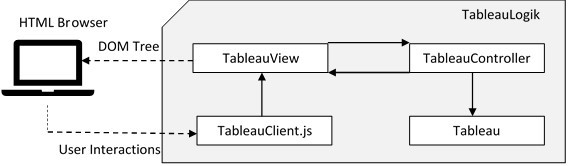
\includegraphics[width=1.0\textwidth]{Achitectur}
\caption[Achitektur]{Achitektur}\label{fig:Achitectur}
\end{figure}
Abbildung \ref{fig:Achitectur} zeigt die Architektur von der Tableau-Webanwendung im Überblick. Die Architektur folgt dem bewährten Model-View-Controller-Prinzip. Softwaretechnisch gliedert sich die
Anwendungslogik so in mehrere Komponenten (Klassen) mit spezifischen funktionalen Verantwortlichkeiten.
%Eine zentrale Rolle für die Anwendungssteuerung hat der Controller (Klasse TableauController). Der Controller kann Nutzerinteraktionen 
%erkennen und in entsprechende Modelinteraktionen umsetzen. Der Controller wird detailliert im Unterabschnitt \ref{subsec:Controller} erläutert.
Die \textit{``TableauClient.js''}
%, die im Unterabschnitt blablabla erläutert
 kann Nutzerinteraktionen erkennen und über den View an den Controller weiterleiten. Der Controller unter entsprechenden Nutzerinteraktionen in 
%Modelinteraktionen 
Model
umsetzen. Der Controller wird detailliert im Unterabschnitt \ref{subsec:Controller} erläutert.

Die \textit{TableauView} kapselt den DOM-Tree und bietet entsprechende Manipulationsmethoden für den Controller an, um sich verändernde Anwendungszustände im Browser zur Anzeige zu bringen. Der View wird im Unterabschnitt \ref{subsec:View} erläutert.

Konzeptionell wird die Tableau-Webanwendung in einem Model abgebildet. Das Model ist komplexer und gliedert sich in mehrere logische Entities, die sich aus den Grundlagen des Kapitels \ref{sec:Grundlagen} ableiten und im Unterabschnitt \ref{sec:Model} erläutert werden.

\section{Klassendiagramm}
Um einen genaueren Überblick zu erhalten, welche Klassen wie mit einander kommunizieren, eignet sich ein Klassendiagramm. Nachfolgend ist zu erkennen, in welcher Kommunikation die Klassen zueinander stehen.
\begin{figure}[ !h] \centering
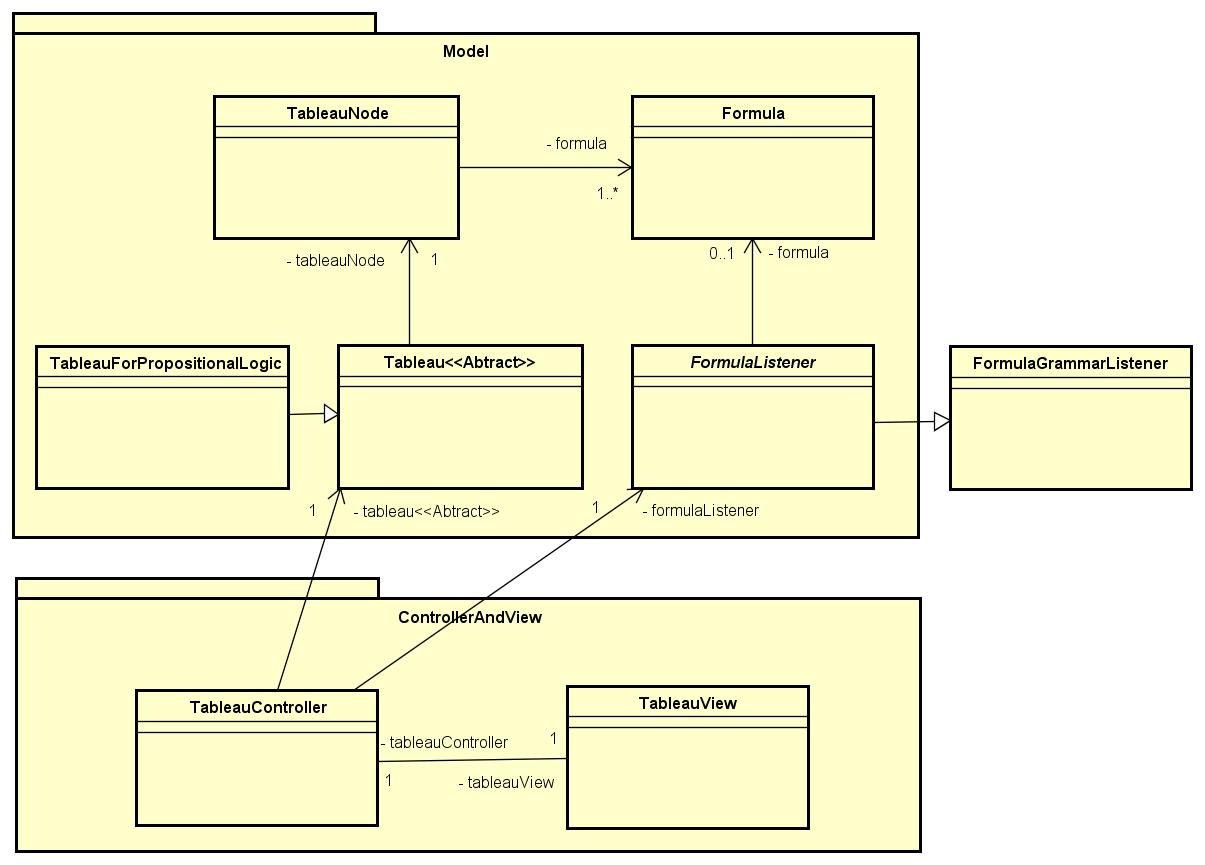
\includegraphics[width=1.0\textwidth]{ClassDiagram}
\caption[Klassendiagramm]{Klassendiagramm}\label{fig:Klassendiagramm}
\end{figure}

Tableau-Webanwendung umfasst verschiedene Bereiche:
\begin{itemize}
\item	Analyse der Eingabeformel und Darstellung einer Formel als Baumstruktur(\hyperlink{/LF10/}{/LF10/}): Klassen \textit{FormulaListener} und \textit{Formula}.
\item	Erstellung und Darstellung des Tableaus (\hyperlink{/LF20/}{/LF20/} und \hyperlink{/LF30/}{/LF30/}):  Klassen \textit{TableauNode}, \textit{Tableau} und \textit{TableauForPropositionalLogic}.
\item	Verarbeitung der GUI-Interaktionen (\hyperlink{/LF10/}{/LF10/}, \hyperlink{/LF20/}{/LF20/}, \hyperlink{/LF30/}{/LF30/} und \hyperlink{/LF40/}{/LF40/}): Klassen \textit{TableauView} und \textit{TableauController}.
\end{itemize}

Um die Möglichkeit zur Erweiterung der Software, gibt es eine abtrakte Klasse \textit{Tableau}, welche die Tableaus erweitern. Die abstrakte Klasse definiert die Basismethoden um ein Tableau zu erstellen. 


%\cleardoublepage
\chapter{Implementierung}\label{sec:Implementierung}
In diesem Kapitel geht es um die Implementierung der Webanwendung. 

Wie im Abschnitt \ref {sec:Antlr4} erwähnt, kann man das Skript \textit {require.js} verwenden um das Importieren von dutzenden Dateien manuell zu vermeiden, wie im folgenden Beispiel gezeigt:

\begin{lstlisting}[language=HTML,basicstyle=\scriptsize]
    <script src="src/Enums.js"></script>
    <script src="src/Model/Formula.js"></script>
    <script src="src/Model/TableauNode.js"></script>   
    <script src="src/Model/TableauForPropositionalLogic.js"></script>
    ...
</body>
</html>
\end{lstlisting}
Diese Dateien müssen in der folgenden Reihenfolge geladen werden:
\begin{itemize}
\item	\textit{Enums.js} muss zuerst geladen werden, da alle anderen Dateien es benötigen.
\item	\textit{Formula.js} wird von \textit{TableauNode.js} verwendet und muss daher zuerst geladen werden.
\item	In ähnlicher Weise wird \textit{TableauNode.js} von \textit{TableauForPropositionalLogic.js} verwendet und muss daher als nächstes geladen werden.
\end{itemize}
Man kann leicht erkennen, dass das Laden von Dateien in der richtigen Reihenfolge wichtig ist, da sie voneinander abhängig sind. Dies mag zunächst kein Problem sein, aber wenn der Code kompliziert wird, wachsen die Dateien und es wird immer schwieriger, die \textit{script}-Tags zu verwalten.

%Wenn man die JavaScript Dateien manuell wie oben importiert, gibt es viele Nachteile wie \footnote{\url{https://frederic-hemberger.de/talks/requirejs/\# /3}}:
%\begin{itemize}
%\item	Websites werden immer komplexer.
%\item	Komplexer Code ist schlechter zu warten.
%\item	Komplexer Code ist schlechter zu testen.
%\item	Verwaltung der Abhängigkeiten von Hand ist fehleranfällig
%\end{itemize}

Daher wird \textit{require.js} im Rahmen dieser Arbeit nicht nur für die ANTLR-Bibliothek sondern für alle andere JavaScript-Dateien verwendet. \textit{require.js} implementiert die Funktion \textit{require()} von \textit{Node.js} im Browser. \textit{require()} wird zum Laden von Dateien verwendet. Für normale JavaScript-Dateien bedeutet dies, dass sie ausgeführt werden, wenn sie zum ersten Mal geladen werden, und das war es. Der Code wird in seiner eigenen Schließung ausgeführt, so dass er den Rest des Codes nicht stört (z.B. identische Variablennamen sind kein Problem). Die einzige Möglichkeit, etwas an die Außenwelt zurückzugeben, besteht darin, ein spezielles Objekt \textit{exports}, das aufgerufen wird, zu ändern , wobei dies der Rückgabewert des\textit{ require()} Aufrufs ist. Eine JavaScript-Datei, die \textit{exports} eine Funktion oder Variable an die Außenwelt zurückgibt, wird als ``Modul'' bezeichnet \cite{pixels}. Man kann \textit{require()} in seinem Browser wie folgt verwenden:

\begin{lstlisting}[language=HTML,basicstyle=\scriptsize]
<html>
<head>
	<script type="text/javascript" src="lib/require.js"></script>
</head>
<body>
	<script type="text/javascript">
		var Formula = require("src/Model/Formula.js").Formula;
		var formula =  new Formula("1", null, null, FormulaTypeEnum.TRUE);
		var type = formula.getFormulaType();
	</script>
</body>
</html>
\end{lstlisting}
Der Code in \textit{Formula.js} könnte so aussehen:
\begin{lstlisting}[language=JavaScript,basicstyle=\scriptsize]
function Formula(label, left, right, formulaType) {
    this.right = right;
    this.left = left;
    this.label = label;
    this.formulaType = formulaType;
}
Formula.prototype.getFormulaType = function () {
    return this.formulaType;
};

exports.Formula = Formula;
\end{lstlisting}

Die einzige Datei, die man normalerweise laden muss, ist \textit{require.js}, die definiert \textit{window.require()}. Danach kann man das Modul \textit{Formula.js} wie in \textit{Node.js} laden. Die Variable \textit{Formula} enthält alle vom Modul exportierten Daten, so dass man sich diese als ``Namespace'' vorstellen kann. Das Aufrufen einer exportierten Funktion \textit{getFormulaType()} in diesem Fall, funktioniert genauso wie das Aufrufen der Methode eines Objekts. Von hier werden alle exportierten Funktionen als ``Methoden'' bezeichnet.

Im Rahmen dieser Arbeit werden alle sogenannten ``Namespaces'' im Skript \textit{Global.js} definiert. Weiterhin enthält das Skript auch alle globalen Variablen der Anwendung.

\begin{itemize}
\item \textit{view}: globale Instanz der Klasse \textit{TableauView}
\item \textit{InputError}: Boolean Variable, ist ``true'' wenn es eine Antlr-Fehlermeldung gibt.
\item \textit{ErrorMessage}: Ein Array um die Antlr-Fehlermeldungen zu speichern.
\item \textit{TableauChartData}: ``Google Charts DataTable'' um das Tableau zu visualisieren.
\item \textit{ArrOfTableauNodesByStepByStep}: Ein Array speichert die Tableau-Knoten für den Tableau-Chart in einem Schritt der ``Schritt für Schritt Lösung'' (wird in der Methode drawTableauChartStepByStep() verwendet).
\item \textit{ArrOfAllTableauNodes}: Ein Array speichert die übrige Tableau-Knoten, die noch nicht für den Tableau-Chart der ``Schritt für Schritt Lösung'' benutzt werden (wird in der Methode drawTableauChartStepByStep() verwendet). 
\item \textit{TableauStepByStepData}: ``Google Charts DataTable'' um das Tableau für die ``Schritt für Schritt Lösung'' zu visualisieren.
\item \textit{stepNr}: Ordnungszahl des aktuellen Schrittes (wird für ``Schritt für Schritt Lösung'' verwendet).
\item \textit{chartNr}: Ordnungszahl des aktuellen Organigramm (wird für ``Schritt für Schritt Lösung'' verwendet).
\item \textit{nexStepNr}: Ordnungszahl des nächsten Schrittes (wird für ``Schritt für Schritt Lösung'' verwendet).
\item \textit{isTautology}:  Ergebnis der Tautologie-Prüfung. Die Variable wird in der Enumeration \textit{TautologyOrSatisfiableEnum} definiert (default: \textit{TautologyOrSatisfiableEnum.NOTTESTED}, wenn die Tautologie nicht geprüft wird).
\item \textit{isSatifiable}:   Ergebnis der	Erfüllbarkeit-Prüfung. Die Variable wird in der Enumeration \textit{TautologyOrSatisfiableEnum} definiert (default: \textit{TautologyOrSatisfiableEnum.NOTTESTED}, wenn die Erfüllbarkeit nicht geprüft wird).
\begin{lstlisting}[language=JavaScript, caption= TautologyOrSatisfiableEnum,basicstyle=\scriptsize]
const TautologyOrSatisfiableEnum = Object.freeze({
    TRUE: "TRUE",
    FALSE: "FALSE",
    NOTTESTED: "NOTTESTED"
});
exports.TautologyOrSatisfiableEnum = TautologyOrSatisfiableEnum;
\end{lstlisting}
\end{itemize}
	\section{Struktur Dateisystem}
Die Struktur der Dateien ist klar getrennt (Abbildung \ref{fig:Ordnerstruktur}).
\begin{figure}[ !h] \centering
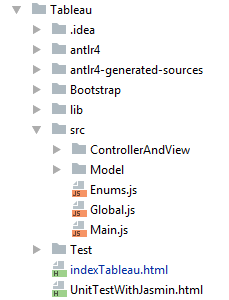
\includegraphics[]{Ordnerstruktur}
\caption[Ordnerstruktur]{Ordnerstruktur}\label{fig:Ordnerstruktur}
\end{figure}

In dem \textit{``Tableau''} Ordner liegen alle Dateien, welche in die Seite eingebunden werden. Dazu zählt ANTLR- und Bootstrap-Framework, generierte Dateien von ANTLR, Bibliothek, JavaSript Dateien und Test. Neben dem Ordner liegen weitere 
Html Dateien. Dazu zählt die 
%Dateien wie die statische Seite. Die Statische Seite ist eine einfache HTML-Datei 
\textit{``indexTableau.html''}, welche durch eingebundenes JavaScript interaktiv mit dem Anwender interagiert. Für das Testen des JavaScripts bietet es sich an, die HTML-Dateien \textit{``UnitTestModel.html''} und \textit{``UnitTestControllerView.html''}zu erstellen, die zusätzlich die Testfälle beinhaltet.

Der \textit{``antlr4-generated-soures''} Ordner (Abbildung \ref{fig:antlr4-generated-sources Ordner}) erhält die ANTLR-Runtime, BAT-Datei um die Runtime auszuführen, Grammatik der aussagenlogischen Formeln und alle Dateien wie  Token, Lexer, Parser, Listener und Visitor, welche die ANTLR-Runtime generiert hat.
\begin{figure}[ !h] \centering
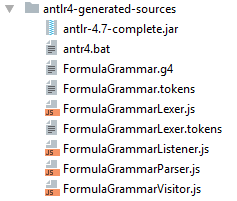
\includegraphics[]{antlr4GeneratedSources}
\caption[Ordnerstruktur antlr4GeneratedSources]{antlr4GeneratedSources}\label{fig:antlr4-generated-sources Ordner}
\end{figure}

Der \textit{``lib''} Ordner (Abbildung \ref{fig:libOrdner}) erhält die Jasmine-Bibliothek und \textit{``require.js''}.
\begin{figure}[ !h] \centering
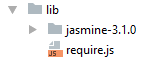
\includegraphics[]{lib}
\caption[Ordnerstruktur lib]{lib}\label{fig:libOrdner}
\vspace*{0.3cm}
\end{figure}

Für die Funktionalität der Webanwendung sorgen die JavaScript-Dateien aus dem \textit{``src''} Ordner (Abbildung \ref{fig:srcOrdner}). Dazu zählt das Model, Controller und View sowie alle Enumerationen, globale Variable und ``Namespaces''.
\begin{figure}[ !h] \centering
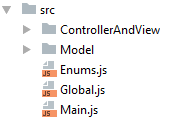
\includegraphics[]{src}
\caption[Ordnerstruktur src]{src}\label{fig:srcOrdner}
\vspace*{0.3cm}
\end{figure}

Zur Qualitätssicherung gibt es Unit-Tests. Diese liegen unterhalb des ``Tests'' Ordners (Abbildung \ref{fig:testOrdner}).
\begin{figure}[ !h] \centering
\includegraphics[]{test}
\caption[Ordnerstruktur test]{test}\label{fig:testOrdner}
\vspace*{0.3cm}
\end{figure}

	\section{FormulaGrammar.g4}
Aus dem Unterabschnitt \ref{subsec:FormelGrammatik} kann eine Formel als Strings, die über eine kontextfreie formale Grammatik generiert wird, definiert werden. Das Alphabet der Formel, das in der Definition \ref{Definition 2.1} definiert wird, wird wie folgt implementiert.
\begin{itemize}
\item Die Aussagenvariable kann beliebige große und kleine Buchstaben enthalten.

\begin{lstlisting}[language=Grammar, basicstyle=\scriptsize]
ATOM: [a-zA-Z];
\end{lstlisting}
\item Basierend auf dem Unterabschnitt \ref{subsec:Notation} werden die folgenden Notationen der Junktoren verwendet:

\begin{lstlisting}[language=Grammar, basicstyle=\scriptsize]
NEG : '!';    // negation
IMP : '=>';   // implication		
EQU: '<=>';   // equivalence
XOR: '^';     // exclusive or
AND : '&';    // conjunction
NAND : '!&';  // nand
OR : '|';     // disjunction
NOR : '!|';   // nor
\end{lstlisting}

\item Die Konstanten kann 0, 1 , true oder false (in ``case-insensitive'') sein.

\begin{lstlisting}[language=Grammar, basicstyle=\scriptsize]
TRUE: (T R U E| '1'); 
FALSE: (F A L S E| '0');
fragment T : [tT]; // match either an 't' or 'T'
fragment R : [rR];
fragment U : [uU];
fragment E : [eE];
...
\end{lstlisting}
\end{itemize}

ANTLR löst Mehrdeutigkeiten zugunsten der zuerst genannten Alternative. Aus den Bindungsregeln in dem Unterabschnitt \ref{subsec:Bindungskonventionen} hat 
die Regel \textit{expr} z.B die Konjuktionsalternative vor der Disjunktionsalternative. Die Produktionen von der Grammatik der aussagenlogischen Formeln wird wie folgt implementiert: 

\begin{lstlisting}[language=Grammar, basicstyle=\scriptsize]
stat :	expr EOF;
expr :	NEG expr                     # Negation
		| expr op=('&'|'!&') expr        # AndNand
		| expr op=('|'|'!|') expr        # OrNor		
		| expr '=>' expr                 # Implication	
		| expr op=('<=>'|'^') expr       # EquXor							
		| ATOM                           # Atom
		| TRUE                           # True
		| FALSE                          # False
		| '(' expr ')'                   # Parens
		;
\end{lstlisting}


Dazu sind ``\# Negation'', ``\# AndNand'' usw. die Bezeichnungen von der Alternativen der Regel \textit{expr}. Diese Bezeichnungen erscheinen am rechten Rand von Alternativen und beginnen mit dem \# -Zeichen.
	\section{Model}\label{sec:Model}
Das Model repräsentiert die zugrunde liegende logische Struktur von Daten in der Tableau-Anwendung. Das Klassendiagramm des Models ist in Abbildung \ref{fig:KlassendiagrammModel} gezeigt.

\begin{figure}[!h] \centering

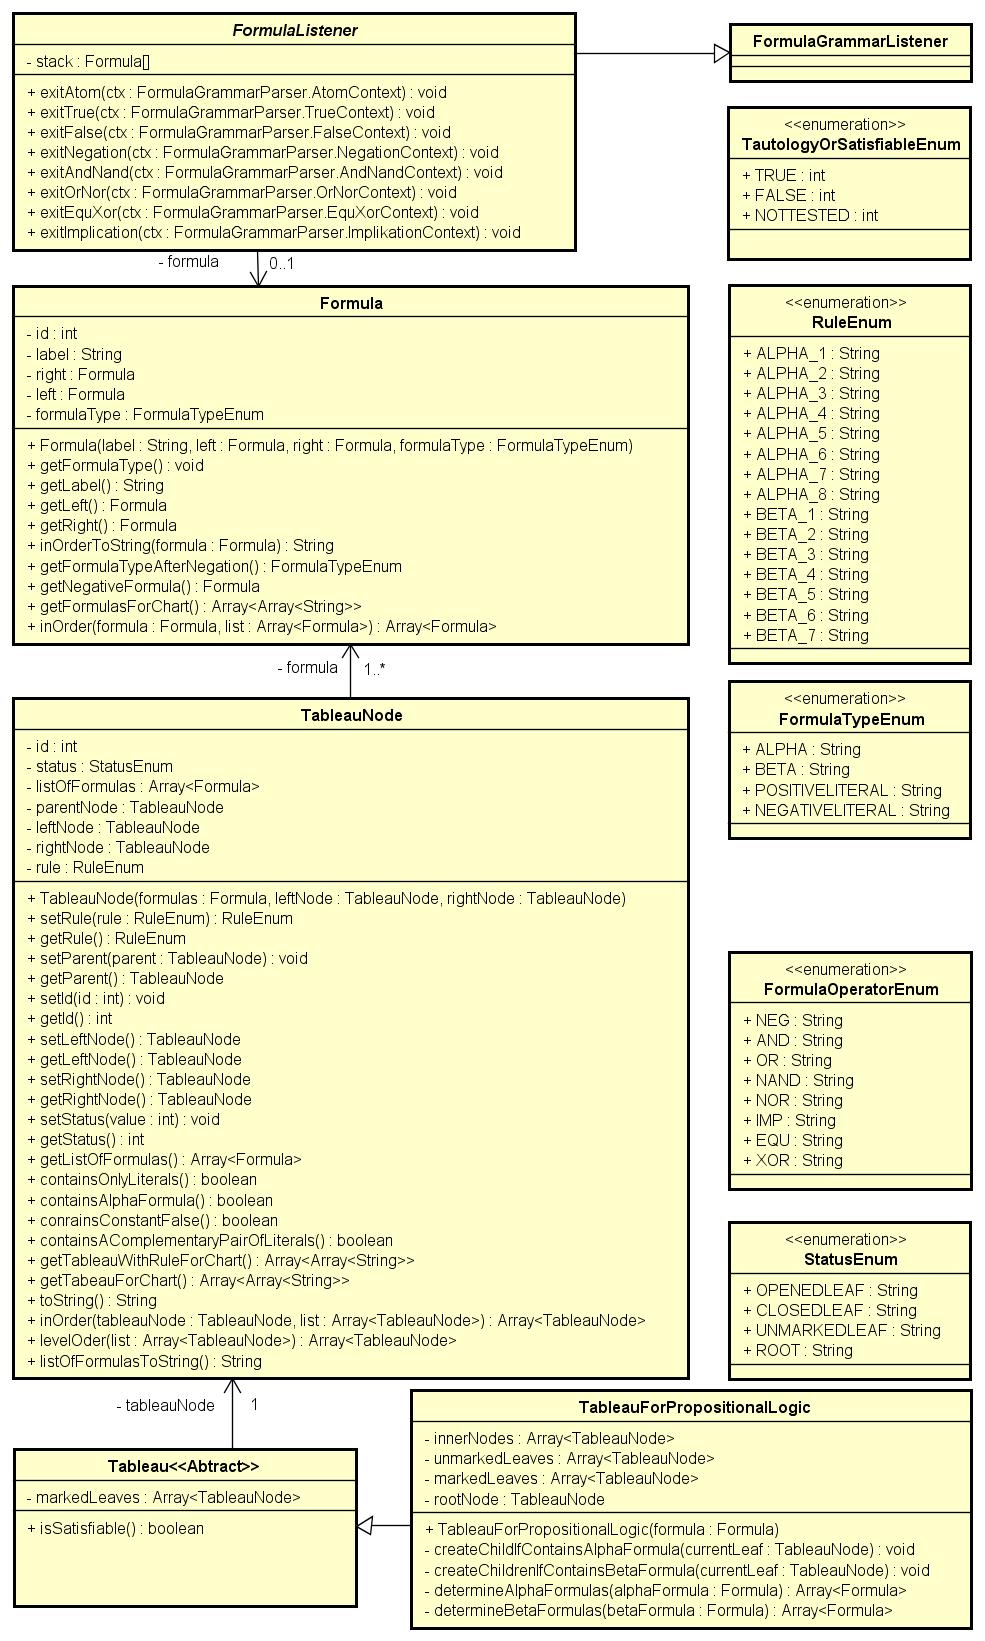
\includegraphics[width=0.9\textwidth]{ClassDiagramModel}
\caption[KlassendiagrammModel]{Klassendiagramm(Model)}\label{fig:KlassendiagrammModel}

\end{figure}

\subsection{Formula}
Aus der Definition \ref{Definition 2.2} ist es möglich, dass jede Formel als ein Binärbaum dargestellt werden kann. Der Baum besteht aus Knoten (\textit{Formula}). Jeder Knoten hat einen linken Teilbaum (\textit{left}), einen rechten Teilbaum (\textit{right}), die auch Knoten sind und einen Inhalt (\textit{label}), welcher eine Aussagenvariable oder ein Junktor (Definition \ref{Definition 2.1}) ist \cite{Krohn}. Die Junktoren werden in der Enumeration \textit{FormulaOperatorEnum} definiert.
\begin{lstlisting}[language=JavaScript, caption= FormulaOperatorEnum, basicstyle=\scriptsize]
const FormulaOperatorEnum = Object.freeze({
    NEG: "\u00AC",
    AND: "\u2227",
    OR:  "\u2228",
    NAND:"\u2191",
    NOR: "\u2193",
    IMP: "\u2192",
    EQU: "\u2194",
    XOR: "\u2295"
});
exports.FormulaOperatorEnum = FormulaOperatorEnum;
\end{lstlisting}

Weiterhin kann eine Formel ein Literal (Definition \ref{Definition 2.57}), $\alpha$- oder $\beta$-Formel (Tabelle \ref{Abb. 2.8}) sein. Diese Formeltypen werden in der Enumeration \textit{FormulaTypeEnum} definiert und werden in dem Attribut \textit{formulaType} der Klasse \textit{Formula} gespeichert. Aus der Bemerkung \ref{FormelAlsString} kann der Ausdruck als String von einer Formel durch eine In-order-Baumtraversierung erhalten werden. Um diesen Ausdruck korrekt abzubilden (z.B. $\neg$q nicht q$\neg$), hat die Formel, die mit einer $\neg$ (oder \textit{FormulaOperatorEnum.NEG}) gekennzeichnet wird, immer nur ein rechtes Kind, d.h \textit{left} ist ``\textit{Null}''. Wenn eine Formel ein Blatt ist, sind beide (\textit{left} und \textit{right}) auch ``\textit{Null}''. Damit die Formel mittels Google Charts visualisiert werden kann (Unterabschnitt \ref{Organigramm}), muss jeder Knoten eine eindeutige Kennzeichnung (\textit{id}) haben.

\begin{lstlisting}[language=JavaScript, caption= FormulaTypeEnum, basicstyle=\scriptsize]
const FormulaTypeEnum = Object.freeze({
    ALPHA: "ALPHA",
    BETA: "BETA",
    NEGATIVLITERAL: "NEGATIVLITERAL",
    POSITIVLITERAL: "POSITIVLITERAL",
    TRUE: "TRUE",
    FALSE: "FALSE"
});
\end{lstlisting}

Um die Tautologie einer Formel zu überprüfen, benötigt es die Negation der Formel. Daher bietet Klasse \textit{Formula} die Methode \textit{getNegativeFormula()}. Nach der Negation wird der Formeltyp geändert, deshalb wird die Methode \textit{getFormulaTypeAfterNegation()} implementiert, um den neuen Formeltyp zu bestimmen.

\begin{lstlisting}[language=JavaScript, caption= getNegativeFormula() und getFormulaTypeAfterNegation() (Klasse Formula) , basicstyle=\scriptsize]
Formula.prototype.getFormulaTypeAfterNegation = function () {
    var formulaType;
    if (this.getFormulaType() == FormulaTypeEnum.TRUE) {
        formulaType = FormulaTypeEnum.FALSE;
    } else if (this.getFormulaType() == FormulaTypeEnum.FALSE) {
        formulaType = FormulaTypeEnum.TRUE;
    } else if (this.getFormulaType() == FormulaTypEnum.POSITIVLITERAL) {
        formulaType = FormulaTypeEnum.NEGATIVLITERAL;
    } else if (this.getLabel() == FormulaOperatorEnum.NEG) {
        formulaType = FormulaTypeEnum.ALPHA;
    } else if (this.getFormulaType() == FormulaTypeEnum.ALPHA) {
        formulaType = FormulaTypeEnum.BETA;
    } else {
        formulaType = FormulaTypeEnum.ALPHA;
    }
    return formulaType;
};

Formula.prototype.getNegativeFormula = function () {
    var negationFormulaType = this.getFormulaTypeAfterNegation();
    var negationFormula = new Formula(FormulaOperatorEnum.NEG, null, this, negationFormulaType);
    return negationFormula;
};
\end{lstlisting}

Außerdem bietet Klasse \textit{Formula} die folgenden Methoden:
\begin{itemize}
\item	\textit{inOrder()}: Rekusive Methode, die eine Liste der Knoten durch In-Order-Baumtraversierung zurück gibt. 
\item	\textit{inOrderToString()}: Gibt Ausdruck als String von der Formel zurück.
\item	\textit{getFormulasForChart()}: Erzeugt ``Google Charts DataTable'' um die Formel zu visualisieren. Die DataTable ist ein zweidimensionales Array. Jedes Element des Arrays beschreibt einen Knoten mit \textit{id} des Knotens und der \textit{id} des übergeordneten Knotens. Diese Ids werden nicht angezeigt. Im Diagramm wird nur das \textit{label} des Knotens angezeigt. Alle Elemente des Arrays werden durch In-Order-Baumtraversierung sortiert.
\end{itemize}

\begin{lstlisting}[language=JavaScript, caption= getFormulasForChart()(Klasse Formula), basicstyle=\scriptsize]
Formula.prototype.getFormulasForChart = function () {
    var ret = [];
    var list = [];
    var arr = [];
    list = this.inOrder(this, list);
    for (var i = 0; i < list.length; i++) {
        list[i].id = i;
    }
    ret.push([{v: this.id.toString(), f: this.label}, ""]);
    for (var i = 0; i < list.length; i++) {
        if (list[i].left != null) {
            arr = [{v: list[i].left.id.toString(), f: list[i].left.label}, list[i].id.toString()];
            ret.push(arr);
        }
        if (list[i].right != null) {
            arr = [{v: list[i].right.id.toString(), f: list[i].right.label}, list[i].id.toString()];
            ret.push(arr);
        }
    }
    return ret;

};
\end{lstlisting}

\subsection{FormulaListener}
Mit ANTLR kann man den Parse-tree mit einem benutzerdefinierten Listener oder einem benutzerdefinierten Visitor besuchen.
Beide Implementierungen geben dasselbe Ergebnis aus. Die Visitor-Implementierung hat aber einen Vorteil, da die Visitor-Methoden einen Wert zurück geben und keine Werte in Feldern gespeichert werden müssen. Dagegen wird die Listener-Implementierung in dieser Arbeit gewählt, da diese im JavaScript bekannter ist und es viele Beispiele im Internet sowie auf der offiziellen Seite \url{https://github.com/antlr/antlr4/blob/master/doc/javascript-target.md} gibt.

\textit{FormulaListener} definiert einen benutzerdefinierten Listener um die Syntaxbaum zu besuchen. Diese Klasse erweitert die Klasse \textit{FormulaGrammarListener}, eine Klasse welche die ANTLR-Runtime automatisch generiert hat.

\begin{lstlisting}[language=JavaScript, caption= FormulaListener Konstruktor, basicstyle=\scriptsize]
 var FormulaListener = function () {
    FormulaGrammarListener.call(this);
};

FormulaListener.prototype = Object.create(FormulaGrammarListener.prototype);
\end{lstlisting}


\textit{FormulaGrammarListener} definiert alle Methoden, die die Klasse \textit{ParseTreeWalker} von der ANTLR-Runtime auslösen kann, wenn sie den Parse-tree durchläuft. Um die Eingabeformel zu analysieren muss man auf acht Ereignisse reagieren, indem man acht Methoden überschreibt: Wenn der Walker eine Aussagenvariable, einen Junktor oder eine Konstante verlässt. Hier sind die relevanten Methoden von der generierten Klassen \textit{FormulaGrammarListener}: 

\begin{lstlisting}[language=JavaScript, caption= FormulaGrammarListener, basicstyle=\scriptsize]
function FormulaGrammarListener() {
	antlr4.tree.ParseTreeListener.call(this);
	return this;
}

FormulaGrammarListener.prototype = Object.create(antlr4.tree.ParseTreeListener.prototype);

FormulaGrammarListener.prototype.constructor = FormulaGrammarListener;
// Exit a parse tree produced by FormulaGrammarParser#Atom.
FormulaGrammarListener.prototype.exitAtom = function(ctx) {};

// Exit a parse tree produced by FormulaGrammarParser#True.
FormulaGrammarListener.prototype.exitTrue = function(ctx) {};

// Exit a parse tree produced by FormulaGrammarParser#False.
FormulaGrammarListener.prototype.exitFalse = function(ctx) {};

// Enter a parse tree produced by FormulaGrammarParser#Negation.
FormulaGrammarListener.prototype.enterNegation = function(ctx) {};

// Exit a parse tree produced by FormulaGrammarParser#AndNand.
FormulaGrammarListener.prototype.exitAndNand = function(ctx) {};

// Exit a parse tree produced by FormulaGrammarParser#OrNor.
FormulaGrammarListener.prototype.exitOrNor = function(ctx) {};

// Exit a parse tree produced by FormulaGrammarParser#EquXor.
FormulaGrammarListener.prototype.exitEquXor = function(ctx) {};

// Exit a parse tree produced by FormulaGrammarParser#Implication.
FormulaGrammarListener.prototype.exitImplikation = function(ctx) {};

\end{lstlisting}

Da Listener-Methoden keinen Wert zurück geben, muss \textit{FormulaListener} ein Array \textit{stack} um die besuchende Formeln zu speichern, haben. Weiterhin hat \textit{FormulaListener} folgende überschriebenen Methoden. Jede Methode hat ein Argument \textit{ctx}. Das Argument ctx ist eine Instanz eines spezifischen Klassenkontextes für den Knoten, den Walker verlässt.

\begin{itemize}

\item	\textit{exitAtom()}: Diese Methode fügt eine neue Aussagenvariable im \textit{stack} hinzu wenn der Walker eine \textit{Atom}-Regel verlässt.
\begin{lstlisting}[language=JavaScript, caption= exitAtom() (Klasse FormulaListener), basicstyle=\scriptsize]
FormulaListener.prototype.exitAtom = function (ctx) {
    var label = ctx.ATOM().getText();
    var formula = new Formula(label, null, null, FormulaTypeEnum.POSITIVLITERAL);
    this.stack.push(formula);
};
\end{lstlisting}

\item	\textit{exitTrue()}: Diese Methode fügt eine neue Konstante ``true'' im \textit{stack} hinzu wenn der Walker eine \textit{True}-Regel verlässt.
\begin{lstlisting}[language=JavaScript, caption= exitTrue() (Klasse FormulaListener), basicstyle=\scriptsize]
FormulaListener.prototype.exitTrue = function (ctx) {
    var label = ctx.TRUE().getText().toLowerCase();
    var formula = new Formula(label, null, null, FormulaTypeEnum.TRUE);
    this.stack.push(formula);
};
\end{lstlisting}

\item	\textit{exitFalse()}: Analog wie \textit{exitTrue()}. 

\item 	\textit{exitNegation()}: Diese Methode fügt eine negierte Formel im \textit{stack} hinzu wenn der Walker eine \textit{Negation}-Regel verlässt.
\begin{lstlisting}[language=JavaScript, caption= exitNegation() (Klasse FormulaListener), basicstyle=\scriptsize]
FormulaListener.prototype.exitNegation = function (ctx) {
    var label = FormulaOperatorEnum.NEG;
    var formula;
    var right = this.stack.pop();
    if (right.getFormulaType() == FormulaTypeEnum.TRUE) {
        formula = new Formula(label, null, right, FormulaTypeEnum.FALSE);
    } else if (right.getFormulaType() == FormulaTypeEnum.FALSE) {
        formula = new Formula(label, null, right, FormulaTypeEnum.TRUE);
    } else if (right.getFormulaType() == FormulaTypeEnum.POSITIVLITERAL) {
        formula = new Formula(label, null, right, FormulaTypeEnum.NEGATIVLITERAL);
    } else if (right.getLabel() == FormulaOperatorEnum.NEG) {
        formula = new Formula(label, null, right, FormulaTypeEnum.ALPHA);
    } else if (right.getFormulaType() == FormulaTypeEnum.ALPHA) {
        formula = new Formula(label, null, right, FormulaTypeEnum.BETA);
    } else {
        formula = new Formula(label, null, right, FormulaTypeEnum.ALPHA);
    }
    this.stack.push(formula);
};
\end{lstlisting}

\item	\textit{exitAndNand()}: Diese Methode fügt eine neue Formel im \textit{stack} hinzu wenn der Walker eine \textit{AndNand}-Regel verlässt.
\begin{lstlisting}[language=JavaScript, caption= exitAndNand() (Klasse FormulaListener), basicstyle=\scriptsize]
FormulaListener.prototype.exitAndNand = function (ctx) {
    var formula;
    var right = this.stack.pop();
    var left = this.stack.pop();
    if (ctx.op.type == FormulaGrammarParser.AND) {
        ;
        formula = new Formula(FormulaOperatorEnum.AND, left, right, FormulaTypeEnum.ALPHA);
    } else {
        formula = new Formula(FormulaOperatorEnum.NAND, left, right, FormulaTypeEnum.BETA);
    }
    this.stack.push(formula);
};
\end{lstlisting}

\item \textit{exitOrNor()}, \textit{exitEquXor()} und \textit{exitImplication()}: Analog wie \textit{exitAndNand()}.
\end{itemize}

\subsection{TableauNode}
Die Klasse \textit{TableauNode} ist analog wie \textit{Formula} als ein Binärbaum dargestellt (Definition \ref{Def.Tableau}). Ein Tableau-Knoten hat einen übergeordneten Knoten \textit{(parentNode}), einen linken Teilbaum (\textit{leftNode}), einen rechten Teilbaum (\textit{rightNode}), eine eindeutige Kennzeichnung (\textit{id}) um die Darstellung mittels Google Charts visualisieren zu können und eine Regel-Bezeichnung (\textit{rule}), die in der Enumeration \textit{RuleEnum} definiert. 
\begin{lstlisting}[language=JavaScript, caption= RuleEnum, basicstyle=\scriptsize]
const RuleEnum = Object.freeze({
    ALPHA_1: "a1",
    ALPHA_2: "a2",
    ALPHA_3: "a3",
    ALPHA_4: "a4",
    ALPHA_5: "a5",
    ALPHA_6: "a6",
    ALPHA_7: "a7",
    ALPHA_8: "a8",
    BETA_1: "b1",
    BETA_2: "b2",
    BETA_3: "b3",
    BETA_4: "b4",
    BETA_5: "b5",
    BETA_6: "b6",
    BETA_7: "b7"
});
exports.RuleEnum = RuleEnum;
\end{lstlisting}
Jeder \textit{TableauNode} wird mit einem Array von Formeln (\textit{listOfFormulas}) beschriftet. 
Falls \textit{listOfFormulas} nur die Eingabeformel enthält, dann hat der Tableau-Knoten keinen \textit{parentNode}. In jedem Fall hat er einen, zwei oder keinen untergeordneten Knoten. Wenn er nur einen untergeordneten Knoten hat, ist \textit{leftNode} ``\textit{Null}''.
Außerdem erhält der Tableau-Knoten einen Zustand (\textit{status}), die in der Enumeration \textit{StatusEnum} definiert. Da Tableau ein Baum ist, ist ein \textit{TableauNode} eine Wurzel (\textit{\textit{StatusEnum.ROOT}}) oder ein Blatt. Wenn es ein Blatt ist, dann kann es ein unmarkiertes (\textit{StatusEnum.UNMARKEDLEAF}), offenes (\textit{StatusEnum.OPENEDLEAF}) oder geschlossenes Blatt (\textit{StatusEnum.CLOSEDLEAF}) sein (Algorithmus \ref{Algorithmus 2.64}). 

\begin{lstlisting}[language=JavaScript, caption= StatusEnum, basicstyle=\scriptsize]
const StatusEnum = Object.freeze({
    OPENEDLEAF: "OPENEDLEAF",
    CLOSEDLEAF: "CLOSEDLEAF",
    UNMARKEDLEAF: "UNMARKEDLEAF",
    ROOT: "ROOT"
});
exports.StatusEnum = StatusEnum;
\end{lstlisting}

Ein \textit{TableauNode} kann:
\begin{itemize}
\item	mittels Methode \textit{containsOnlyLiterals()} überprüfen, ob er nur die Literalen erhält.
\begin{lstlisting}[language=JavaScript, caption= containsOnlyLiterals() (Klasse TableauNode), basicstyle=\scriptsize]
TableauNode.prototype.containsOnlyLiterals = function () {
    for (var i = 0; i < this.listOfFormulas.length; i++) {
        if (this.listOfFormulas[i].getFormulaType() == FormulaTypeEnum.ALPHA || this.listOfFormulas[i].getFormulaType() == FormulaTypeEnum.BETA) {
            return false;
        }
    }
    return true;
};
\end{lstlisting}
\item	mittels Methode \textit{containsAlphaFormula()} überprüfen, ob er mindestens eine $\alpha$-Formel erhält. 
\begin{lstlisting}[language=JavaScript, caption= containsAlphaFormula() (Klasse TableauNode), basicstyle=\scriptsize] 
TableauNode.prototype.containsAlphaFormula = function () {
    for (var i = 0; i < this.listOfFormulas.length; i++) {
        if (this.listOfFormulas[i].getFormulaType() == FormulaTypeEnum.ALPHA) {
            return true;
        }
    }
    return false;
};
\end{lstlisting}
\item	mittels Methode \textit{containsConstantFalse()} überprüfen, ob er mindestens eine Konstante 0 der ``false'' (\textit{FormulaTypeEnum.FALSE})  erhält. 
\begin{lstlisting}[language=JavaScript, caption= containsConstantFalse() (Klasse TableauNode), basicstyle=\scriptsize] 
TableauNode.prototype.containsConstantFalse = function () {
    for (var i = 0; i < this.listOfFormulas.length; i++) {
        if (this.listOfFormulas[i].getFormulaType() == FormulaTypeEnum.FALSE) {
            return true;
        }
    }
    return false;
};
\end{lstlisting}
\item	mittels Methode \textit{containsAComplementaryPairOfLiterals()} überprüfen, ob er mindestens ein komplementäres Paar erhält. 
\begin{lstlisting}[language=JavaScript, caption= containsConstantFalse() (Klasse TableauNode), basicstyle=\scriptsize]
TableauNode.prototype.containsAComplementaryPairOfLiterals = function () {
    var positiveLiterals = [];
    var negativeLiterals = [];
    for (var i = 0; i < this.listOfFormulas.length; i++) {
        if (this.listOfFormulas[i].getFormulaType() == FormulaTypeEnum.POSITIVLITERAL) {
            if (negativeLiterals.length == 0) {
                positiveLiterals.push(this.listOfFormulas[i]);
            }
            for (var j = 0; j < negativeLiterals.length; j++) {
                if (negativeLiterals[j].label == this.listOfFormulas[i].getLabel()) {
                    return true;
                } else {
                    positiveLiterals.push(this.listOfFormulas[i]);
                }
            }
        } else if (this.listOfFormulas[i].getFormulaType() == FormulaTypeEnum.NEGATIVLITERAL) {
            if (positiveLiterals.length == 0) {
                negativeLiterals.push(this.listOfFormulas[i].getRight());
            }
            for (var h = 0; h < positiveLiterals.length; h++) {
                if (positiveLiterals[h].label == this.listOfFormulas[i].getRight().getLabel()) {
                    return true;
                } else {
                    negativeLiterals.push(this.listOfFormulas[i].getRight());
                }
            }
        }

    }
    return false;
};
\end{lstlisting}
\end{itemize}

Weiterhin bietet Klasse \textit{TableauNode} die folgenden Methoden:
\begin{itemize}
\item	\textit{inOrder()}: Rekusive Methode, die eine Liste der Tableau-Knoten durch In-Order-Baumtraversierung zurück gibt. 
\item	\textit{levelOrder()}: Gibt eine Liste der Tableau-Knoten durch Breitensuche zurück. 
\item	\textit{toString()}: Führt eine In-Order-Baumtraversierung des Tableau-Knotens durch und gibt das Ergebnis als String zurück.
\item	\textit{listOfFormulasToString()}: Gibt alle Formeln, die der Tableau-Knoten erhält, zurück.
\item	\textit{getTableauForChart()}: Erzeugt ``Google Charts DataTable'' um das Tableau zu visualisieren. Die DataTable ist ein zweidimensionales Array. Jedes Element des Arrays beschreibt einen Knoten mit \textit{id} des Knotens und der \textit{id} des übergeordneten Knotens. Diese Ids werden nicht angezeigt. Im Diagramm werden die Formeln, die der Tableau-Knoten erhält, $\times$ oder $\odot$ angezeigt. Alle Elemente des Arrays werden durch In-Order-Baumtraversierung sortiert.
\item	\textit{getTableauWithRuleForChart()}: Analog wie \textit{getTableauForChart()}, gibt es aber noch Regel-Bezeichnungen (\textit{rule}) anzuzeigen. Alle Elemente des Arrays werden durch Breitensuche sortiert, um diese später für die``Schritt für Schritt Lösung'' zu verwenden.
\end{itemize}

\subsection{Tableau}
\textit{Tableau} ist eine abstrakte Klasse, die die Basismethode \textit{isSatisfiable()} bietet. Diese Methode prüft ob das Array des markierten Blattes (\textit{markedLeaves}) ein offenes Blatt enthält. Wenn ja, ist die Eingabeformel erfüllbar, sonst ist sie unerfüllbar.

\begin{lstlisting}[language=JavaScript, caption= isSatisfiable() (Klasse Tableau), basicstyle=\scriptsize] 
Tableau.prototype.isSatisfiable = function(){
    for(var i = 0; i < this.markedLeaves.length; i ++){
        if(this.markedLeaves[i].getStatus() == StatusEnum.OPENEDLEAF){
            return true;
        }
    }
    return false;
};

exports.Tableau = Tableau;
\end{lstlisting}

\subsection{TableauForPropositionalLogic}
\textit{TableauForPropositionalLogic} erweitert die Klasse \textit{Tableau}. Konstruktor der \textit{TableauForPropositionalLogic} Klasse hat ein Argument \textit{formula}, eine Instanz des Klasse \textit{Formula}, die die Eingabeformel implementiert. Dieser Konstruktor setzt die Konstruktion eines semantischen Tableaus für Aussagenlogik (Algorithmus \ref{Algorithmus 2.64}) um. Dazu speichert er die Wurzel des Tableau im Attribut \textit{rootNode}, ein Array des unmarkierten Blattes im Attribut \textit{unmarkedLeaves} und ein Array des markierten Blattes im Attribut \textit{markedLeaves}.
\begin{lstlisting}[language=JavaScript, caption= TableauForPropositionalLogic Konstruktor, basicstyle=\scriptsize] 
function TableauForPropositionalLogic(formula) {
    this.innerNode = [];
    this.unmarkedLeaves = [];
    this.markedLeaves = [];
    var formulasArr = [formula];
    var rootNode = new TableauNode(formulasArr, null, null);
    idNr++;
    rootNode.setId(idNr);
    this.unmarkedLeaves.push(rootNode);
    while (this.unmarkedLeaves.length > 0) {
        var currentLeaf = this.unmarkedLeaves.pop();
        if (currentLeaf.containsOnlyLiterals()) {
            if (currentLeaf.containsAComplementaryPairOfLiterals()|| currentLeaf.containsConstantFalse()) {
                currentLeaf.setStatus(StatusEnum.CLOSEDLEAF);
            } else {
                currentLeaf.setStatus(StatusEnum.OPENEDLEAF);
            }
            this.markedLeaves.push(currentLeaf);
        } else if (currentLeaf.containsAlphaFormula()) {
            this.createChildIfContainsAlphaFormula(currentLeaf);

        } else {
            this.createChildrenIfContainsBetaFormula(currentLeaf);
        }
    }
    if(this.innerNode.length == 0){
        this.rootNode = this.markedLeaves[0];
    }else{
        this.rootNode = this.innerNode[0];
    }
}

TableauForPropositionalLogic.prototype = Object.create(Tableau.prototype);
\end{lstlisting}

Um diese Tableau-Implementierung übersichtlicher zu gestalten und Fehler zu vermeiden, hat \textit{TableauForPropositionalLogic} die folgenden Methoden:
\begin{itemize}
\item	\textit{determineAlphaFormulas()}: implementiert die Zeile \ref{TableauAl_13} des Algorithmus \ref{Algorithmus 2.64}. Dazu erhält sie eine $\alpha$-Formula als Argument. Durch die Berücksichtigung des Hauptoperator sowie die Negation (falls es eine gibt) der Argument-Formel, bestimmt \textit{determineAlphaFormulas()} die entsprechende Regel nach Tabelle \ref{Abb. 2.8} und ermittelt Formeln $\alpha_1$ und $\alpha_2$.
%Wenn sie keine passende Regel findet, gibt sie eine Fehlermeldung ``rule not found'' auf der Konsole, ansonsten gibt sie ein Array, das die Formeln $\alpha_1$, $\alpha_2$ und die verwendete Regel enthält, in Reihenfolge zurück.
\item	\textit{determineBetaFormulas()}:  Analog \textit{determineAlphaFormulas()}, implementiert sie die Zeile \ref{TableauAl_19} des Algorithmus \ref{Algorithmus 2.64}. Diese Methode gibt ein Array, das die Formeln $\beta_1$, $\beta_2$ und die verwendete Regel enthält, in Reihenfolge zurück.
\item 	\textit{createChildIfContainsAlphaFormula()}: Erhält einen Tableau-Knoten \textit{currentLeaf} und implementiert die Zeile \ref{TableauAl_13} bis Zeile  \ref{TableauAl_16} des Algorithmus \ref{Algorithmus 2.64}. Dazu wählt sie die erste  $\alpha$-Formula des \textit{currentLeaf}. Mit dieser Formel kann sie mittels Methode \textit{determineAlphaFormulas()} die Informationen der untergeordneten Knoten (wie $\alpha_1$, $\alpha_2$ und  verwendete Regel), den sie danach erzeugen muss, bekommen. Der untergeordnete Knoten wird mit einem Array der Formeln (\textit{listOfFormula}) beschriftet. Diese Array enthält die Formeln aus \textit{currentLeaf} nach dem Ersetzen der ausgewählten $\alpha$-Formel durch Formeln $\alpha_1$, $\alpha_2$.
\item 	\textit{createChildrenIfContainsBetaFormula()}: Analog wie \textit{createChildIfContainsAlphaFormula()}, implementiert sie die Zeile \ref{TableauAl_19} bis Zeile \ref{TableauAl_24} des Algorithmus \ref{Algorithmus 2.64}. Dazu erzeugt sie mit Hilfe der Methode \textit{determineBetaFormulas()} zwei untergeordnete Knoten von \textit{currentLeaf}. Der linke untergeordnete Knoten (\textit{leftNode}) wird mit einem Array, das die Formeln aus \textit{currentLeaf} nach dem Ersetzen der ausgewählten $\beta$-Formel durch $\beta_1$ enthält, beschriftet. Der rechte untergeordnete Knoten (\textit{rightNode}) wird mit einem Array, das die Formeln aus \textit{currentLeaf} nach dem Ersetzen der ausgewählten $\beta$-Formel durch $\beta_2$ enthält, beschriftet. 
\end{itemize}


	\section{View und Controller}
\subsection{View}\label{subsec:View}
Der View dient der Darstellung der Tableau-Anwendung für den Anwender. Er besteht im Kern aus einem HTML-Dokument (Unterabschnitt \ref{subsubsec:HTML}) und einer clientseitigen Logik, die den DOM-Tree des HTML-Dokuments manipuliert. Die clientseitige Logik hat zwei Bestandteile, also \textit{TableauClient.js} (Unterabschnitt \ref{subsubsec:TableauClient} ) und Klasse \textit{TableauView} (Unterabschnitt \ref{subsubsec:TableauView}).
\subsubsection{HTML-Dokument} \label{subsubsec:HTML}
Das folgendes HTML-Dokument (Listing \ref{lis:HTMLhead} und \ref{lis:HTMLbody}) wird genutzt, um die Anwendung einzublenden. Abbildung  \ref{figs:screenshot-GUI} zeigt dabei einen Screenshot der Anwendung in der Desktop- und Mobile-Version.

\lstinputlisting[language=HTML, caption=HTML-head, basicstyle=\scriptsize, label={lis:HTMLhead}]{head.html}

Diese \textit{head}-Tags enthalten den Titel für benötige Dokumente, Skripte und Metainformationen. In den \textit{link}-Tags wird Bootstrap-Framework und das benutzerdefinierte Stylesheet \textit{style.css} verknüpft. In den \textit{script}-Tags werden die clientseitigen Skripts definiert. Hierbei wird \textit{require.js} verwendet um JS-Dateien zu importieren. \textit{jquery.min.js} und \textit{bootstrap.min.js} werden verwendet um jQuery-Bibliothek und Bootstrap-JavaScript-Plugins einzubinden und \textit{loader.js} wird verwendet um Google-Chart Loader zu laden.

\lstinputlisting[basicstyle=\scriptsize, style=myCustomHTMLStyle, caption=HLML-body, label={lis:HTMLbody}]{body.html}

Wie in Unterabschnitt \ref{Bootstrap} erwähnt, ist die Benutzeroberfläche der Tableau-
Anwendung als eine Responsive-Website mit ``Laptop-First'' Strategie (Bildschirmgröße $\geq$ 768 px) implementiert. Daher wird das Layout der Seite basierend auf der Klasse \textit{.col-md-} von der Bootstrap Grid-System angeordnet und angepasst.

\begin{figure}[ !h] \centering
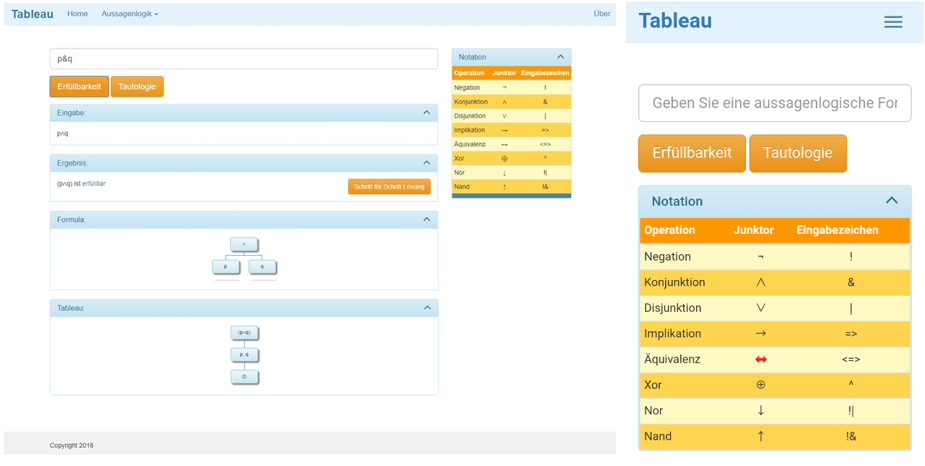
\includegraphics[width=1.0\textwidth]{screenshot-GUI}
\caption[Screenshots der Tableau-Anwendung]{Screenshots der Tableau-Anwendung für Desktop-(links) und Mobile-Version(rechts)}\label{figs:screenshot-GUI}
\end{figure}

\subsubsection{\textit{TableauClient.js} als Schnittstelle zum HTML-Dokument} \label{subsubsec:TableauClient}
Der View wird im Browser initial durch obiges HTML-Dokument erzeugt. Im Verlaufe der Anwendung wird der DOM-Tree dieses HTML-Dokuments durch die Klasse \textit{TableauView} manipuliert, um den Anwendungszustand darzustellen. Die Klasse \textit{TableauView} wird dabei durch das Skript \textit{TableauClient.js}, das die Nutzerinteraktionen ermöglicht, geladen. In dem  Skript \textit{TableauClient.js} werden die folgenden Funktionen implementiert. Hier gibt es eine Beachtung, dass diese Funktionen wie normale JavaScript-Funktionen implementiert werden und nicht vom einem Objekt-Namespace z.B \textit{MyObj.theMethod()} aufgerufen werden.

\begin{itemize}
\item	\textit{pressTautologyButton()}: Diese Funktion wird ausgeführt, wenn der Anwender auf den Button  ``Tautologie'' drückt. Sie initialisiert  eine Instanz der Klasse \textit{TableauView} und ruft die Methode \textit{checkTautology()} der Instanz auf.
\item \textit{pressSatisfiableButton()}: Diese Funktion wird ausgeführt, wenn der Anwender auf den Button  ``Erfüllbarkeit'' drückt. Sie initialisiert eine Instanz der Klasse \textit{TableauView} und ruft die Methode \textit{checkSatisfiable()} der Instanz auf.
\item	\textit{stepByStepSolution()}: Diese Funktion wird ausgeführt, wenn der Anwender auf den Button  ``Schritt für Schritt Lösung'' drückt. Über dem Aufruf der Methode \textit{stepByStepSolutionOutput()} von der Klasse \textit{TableauView} leitet sie diese  Benutzerinteraktion an eine Instanz der Klasse \textit{TableauView} weiter.
\item	\textit{pressNextStepButton()}: Diese Funktion wird ausgeführt, wenn der Anwender auf den Button  ``Nächste Schritt''  mit der Id \textit{nextStepButton} des DOM-Trees  drückt. Über dem Aufruf der Methode \textit{nextSolutionStepOutput()} von der Klasse \textit{TableauView} leitet sie diese Benutzerinteraktion an eine Instanz der Klasse \textit{TableauView} weiter.
\end{itemize}

Außerdem enthält \textit{TableauClient.js} die folgenden Funktionen. Die Funktionen werden von Google Charts unterstützt um die  Organigramme auf der Webseite zeichnet zu lassen. 
\begin{itemize}
\item	\textit{drawFormulaChart()}: Visualisiert die Darstellung der Formel mittels Google Charts. Diese Darstellung wird in das DIV-Element mit der Id \textit{Formula\_chart\_div} des DOM-Trees eingeblendet.
\item	\textit{drawTableauChart()}: Visualisiert die Darstellung des Tableau ohne Regel-Bezeichnungen mittels Google Charts. Diese Darstellung wird in das DIV-Element mit der Id \textit{Tableau\_chart\_div} des DOM-Trees eingeblendet.
\item	\textit{drawTableauChartStepByStep()}: Visualisiert teilweise die Darstellung des Tableau mittels Google Charts.
\item	\textit{drawTableauChartWithRule()}: Visualisiert die Darstellung des Tableau mit Regel-Bezeichnungen mittels Google Charts. Diese Darstellung wird in das DIV-Element mit der Id \textit{stepByStepDiagram} des DOM-Trees eingeblendet.
\begin{lstlisting}[language=JavaScript, caption= drawTableauChart() (TableauClient.js), basicstyle=\scriptsize] 
function drawTableauChart() {
    TableauChartData = new google.visualization.DataTable();
    var arrOfTableauNodes = view.controller.rootTableau.getTableauForChart();
    // For each orgchart box, provide the label, and the parentNode
    TableauChartData.addColumn('string', 'Label');
    TableauChartData.addColumn('string', 'Parent');
    TableauChartData.addRows(arrOfTableauNodes);
    // Create the chart.
    var chart = new google.visualization.OrgChart(document.getElementById('Tableau_chart_div'));
    // Draw the chart, setting the allowHtml option to true for the tooltips.
    chart.draw(TableauChartData, {allowHtml: true});
}
\end{lstlisting}
\end{itemize}

\subsubsection{TableauView} \label{subsubsec:TableauView}
\begin{figure}[ !h] \centering
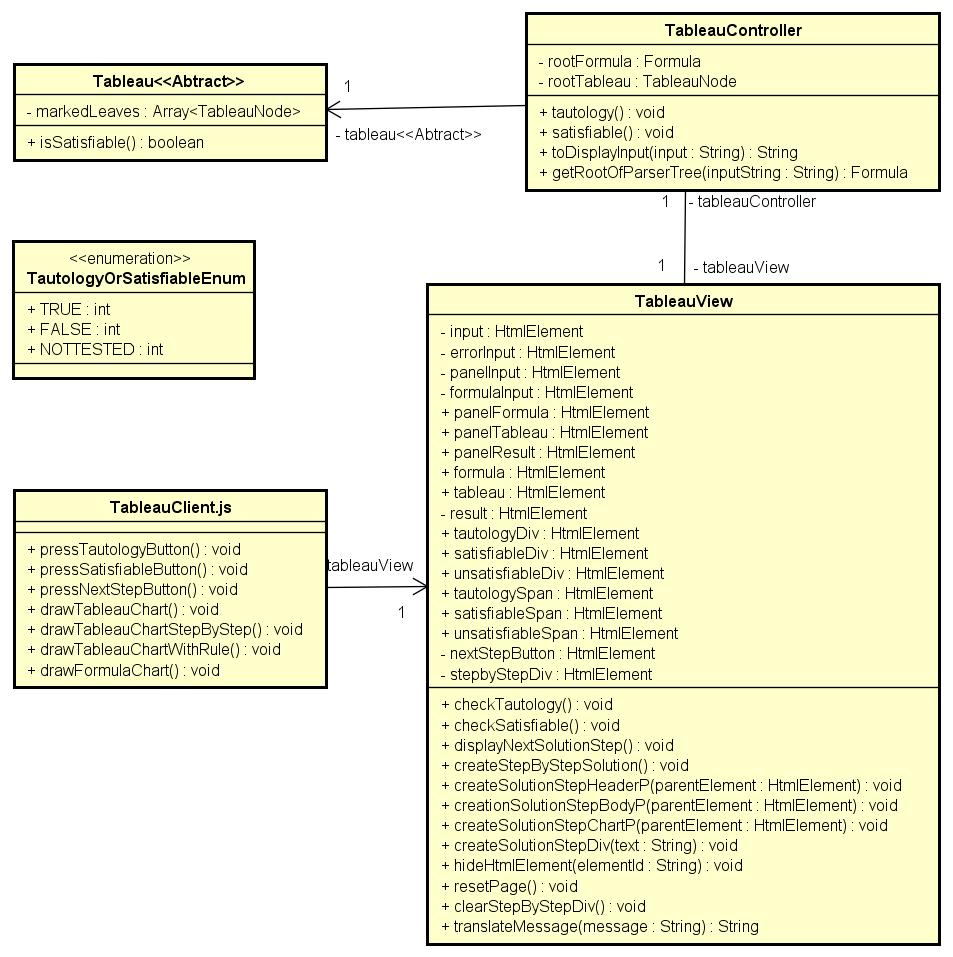
\includegraphics[width=1.0\textwidth]{ClassDiagramViewController}
\caption[KlassendiagrammControllerView]{Klassendiagramm (View und Controller)}\label{fig:KlassendiagrammControllerView}
\end{figure}
Folgende Elemente haben dabei eine besondere Bedeutung und können dabei über entsprechende Attribute der Klasse \textit{TableauView} (Abbildung \ref{fig:KlassendiagrammControllerView}) angesprochen werden.
\begin{itemize}
\item	\textit{input}: Das Element mit dem Identifier \textit{input} dient dazu die Eingabe zu erhalten.
\item	\textit{errorInput}: Das Element mit dem Identifier \textit{errorInput} dient dazu ein Warnungstext bei fehlerhaften Eingaben einzublenden.
\item	\textit{panelInput}: Das Element mit dem Identifier \textit{panel-input} wird genutzt, um die Tafel, die die Eingabeformel enthält, einzublenden.
\item	\textit{formulaInput}: Das Element mit dem Identifier \textit{ formulaInput} dient dazu die Eingabeformel einzublenden.
\item	\textit{panelFormula}, \textit{panelTableau} und\textit{ panelResul}t : Die Elemente mit dem Identifier \textit{panel-formula}, \textit{panel-tableau} und \textit{panel-result} werden genutzt, um die Tafeln, die die Darstellung der Formel, die Darstellung des Tableau und  das Prüfungsergebnis (z.B. dass die Eingabeformel erfüllbar oder Tautologie ist) enthält, einzublenden.
\item	\textit{formula}, \textit{tableau} und \textit{result} : Die Elemente mit dem Identifier \textit{formula}, \textit{tableau} und \textit{resul}t   werden genutzt, um die Panel-Bodys der Panel \textit{panel-formula}, \textit{panel-tableau} und \textit{panel-result} einzublenden.
\item	\textit{tautologyDiv},\textit{ satisfiableDiv} und \textit{unsatisfiableDiv}: Die Elemente mit dem Identifier \textit{tautologyDiv},  \textit{satisfiableDiv}, \textit{unsatisfiableDiv} dient dazu die Prüfungsergebnisse einzublenden.
\item	\textit{tautologySpan}, \textit{satisfiableSpan} und \textit{unsatisfiableSpan}:	Die Element mit dem Identifier  \textit{tautologySpan}, \textit{satisfiableSpan} und  \textit{unsatisfiableSpan} dient dazu die Prüfungsergebnistexte einzublenden.
\item	\textit{nextStepButton}: Das Element mit dem Identifier \textit{nextStepButton} wird genutzt, um das Button ``Nächste Schritt'' im Popup-Fenster ``Schritt für Schritt Lösung'' einzublenden.
\item	\textit{stepByStepDiv}: Das Element mit dem Identifier \textit{stepByStepDiv} wird genutzt, um die Lösung im Popup-Fenster ``Schritt für Schritt Lösung'' einzublenden.
\end{itemize}

\textit{TableauView} kann mittels folgender Methoden den DOM-Tree manipulieren:
\begin{itemize}
\item	\textit{checkTautology()}: Mittels der Methode \textit{toDisplayInput()} des Controllers enthält sie die formatierende Eingabeformel, die in das DIV-Element mit der Id \textit{formulaInput} des DOM-Trees eingeblendet wird. Sie ruft die Methode \textit{tautology()} des Controllers auf um das Tableau und das Ergebnis der Tautologie-Prüfung einzublenden. Bei fehlerhafter Eingaben gibt sie eine Fehlermeldung aus. Diese Fehlermeldung wird in das DIV-Element mit der Id \textit{errorInput} des DOM-Trees eingeblendet.
\begin{lstlisting}[language=JavaScript, caption= checkTautology()(Klasse TableauView), basicstyle=\scriptsize] 
TableauView.prototype.checkTautology = function () {
    this.clearStepByStep();
    var input = this.controller.toDisplayInput(this.input.value);
    this.panelInput.style.display = 'block';
    this.formulaInput.innerHTML = input;
    google.charts.load('current', {packages: ["orgchart"]});
    if (!InputError) {
        this.errorInput.innerHTML = "";
        this.controller.tautology();
    } else {
        var message = "";
        for(var i = 0; i< ErrorMessage.length; i++){
            message += ErrorMessage[i] + ". "
        }
        this.errorInput.innerHTML = "Fehlerhafte Eingabe!\n" + this.translateMessage(message);
        this.resetPage()
    }
    InputError = false;
};
\end{lstlisting}
\item	\textit{checkSatisfiable()}: Analog wie \textit{checkTautology()}, ruft sie die Methode \textit{satisfiable()} des Controllers aus, um das Ergebnis der Erfüllbarkeit-Prüfung auszugeben.
\item	\textit{createSolutionStepChartP()}: Erhält ein HTML-Element und erzeugt in dem Element ein P-Element mit der Id, der mit \textit{``chart-step-''} beginnt und dann mit der Ordnungszahl des Schrittes gefolgt wird. Dieses Element wird verwendet um der ``Chart'' (Abbildung \ref{fig:StepByStepPanelAufbau}) eines Schrittes von der ``Schritt für Schritt Lösung'' einzublenden.
\begin{lstlisting}[language=JavaScript, caption= createSolutionStepChartP(Klasse TableauView), basicstyle=\scriptsize] 
TableauView.prototype.createSolutionStepChartP = function (parentElement) {
    var p = document.createElement("p");
    p.id = "chart-step-" + stepNr;
    p.className = "scroll";
    parentElement.appendChild(p);
};
\end{lstlisting}
\item	\textit{\textit{createSolutionStepDiv()}}: Mit Hilfe der Methoden \textit{createSolutionStepHeader()}, \textit{createSolutionStepBody()},\textit{ createSolutionStepChartP()} erzeugt sie ein DIV-Element mit der Id, der mit \textit{``div-step-''} beginnt und dann mit der Ordnungszahl des Schrittes gefolgt wird, um ein Schritt der ``Schritt für Schritt Lösung'' zu erstellen. Jeder Schritt enthält die Schritt-Nummer (``Header'') die verwendete Regel (``Body''), das Diagramm (``Chart'') und den Hinweis (falls es einen gibt) (Abbildung \ref{fig:StepByStepPanelAufbau}). Diese Methode erhält einen Text, um diesen an die Methode \textit{createSolutionStepBody(}) weiterzuleiten.
\begin{lstlisting}[language=JavaScript, caption= createSolutionStepDiv(Klasse TableauView), basicstyle=\scriptsize] 
TableauView.prototype.createSolutionStepDiv = function (text) {
    var divCurrentStep = document.createElement("div");
    divCurrentStep.id = "div-step-" + stepNr;
    if (divCurrentStep.id != "div-step-1") {
        var pDivider = document.createElement("p");
        pDivider.className = "divider";
        divCurrentStep.appendChild(pDivider);
        divCurrentStep.style.display = 'none';
    }
    this.createSolutionStepHeader(divCurrentStep);
    this.createSolutionStepBody(divCurrentStep, text);
    this.createSolutionStepChartP(divCurrentStep);
    this.stepByStepDiv.appendChild(divCurrentStep);
    google.charts.setOnLoadCallback(drawTableauChartStepByStep);
    stepNr++;
};
\end{lstlisting}
\item	\textit{createStepByStepSolution()}: Mit Hilfe der Methode \textit{createSolutionStepDiv()} erstellt sie die vollständige ``Schritt für Schritt Lösung'' Struktur. Die Tableau-Knoten werden durch Breitensuche sortiert. Die Anzahl der Schritte entspricht der Anzahl der Knotengruppen. Jede Knotengruppe enthält nur die Knoten, die denselben Elternknoten haben. Die Reihenfolge der Schritte entspricht die Reihenfolge der Knoten.
\item	\textit{displayNextSolutionStep()}: Blendet das DIV-Element des nächsten Schrittes ein, wenn es existiert. Dieses Element wird mit der Id, die mit \textit{``div-step-''} beginnt und dann mit der Ordnungszahl des nächsten Schrittes gefolgt wird.
\begin{lstlisting}[language=JavaScript, caption= displayNextSolutionStep(Klasse TableauView), basicstyle=\scriptsize] 
TableauView.prototype.displayNextSolutionStep = function () {
    var nextDivId = "div-step-" + nextStepNr;
    var isNextDivIdExist = document.getElementById(nextDivId);
    if (isNextDivIdExist) {
        document.getElementById(nextDivId).style.display = "block";
    }
    var afterNextDivId = "div-step-" + (nextStepNr + 1);
    var isAfterNextDivIdExist = document.getElementById(afterNextDivId);
    if (!isAfterNextDivIdExist) {
        this.nextStepButton.style.display = "none";
    }
    nextStepNr++;
};
\end{lstlisting}
\end{itemize}

\textit{TableauView} bietet auch die folgende Methoden:
\begin{itemize}
\item	\textit{hideHtmlElement()}: Erhält ein HTML-Element und blendet es aus.
\item	\textit{clearStepByStepDiv()}: Setzt die globale Variablen, die für die ``Schritt für Schritt Lösung''  benötigt werden wie \textit{stepNr}, \textit{nextStepNr}, \textit{chartNr},\textit{ ArrOfTableauNodesByStepByStep}, \textit{ArrOfAllTableauNodes} zurück und blendet den Button ``Nächste Schritt'' aus. Außerdem entfernt sie auch alle untergeordneten Knoten des  \textit{stepByStepDiv} Elements.   
\item	\textit{resetPage()}: Mittels Methode \textit{hideHtmlElement()} und \textit{clearStepByStepDiv(}) blendet sie die HTML-Elemente \textit{panel-result}, \textit{panel-tableau}, \textit{panel-formula} aus und ruft sie die Methode \textit{clearStepByStepDiv()}. Weiterhin löscht sie auch die gespeicherten Fehlermeldungen.
\item	\textit{translateMessage()}: Erhält eine ANTLR-Fehlermeldung und übersetzt sie ins Deutsch.
\end{itemize}


Wenn eine Instanz der Klasse \textit{TableauView} initialisiert wird, initialisiert er auch gleich eine Controller-Instanz. Dieser Controller kann sich hierzu folgender Methoden und Attribute der \textit{TableauView} bedienen, um den DOM-Tree manipulieren zu können:
\begin{itemize}
\item	\textit{createSolutionStepHeaderP()}: Erhält ein HTML-Element und erzeugt in dem Element ein P-Element um die ``Header'' (Abbildung \ref{fig:StepByStepPanelAufbau}) eines Schritt von der ``Schritt für Schritt Lösung'' einzublenden.
\item	\textit{createSolutionStepBodyP()}  Erhält ein Text, ein HTML-Element und erzeugt in dem Element ein P-Element um die ``Body'' (Abbildung \ref{fig:StepByStepPanelAufbau}) eines Schrittes von der ``Schritt für Schritt Lösung'' einzublenden.		
\end{itemize}

Die Abbildung \ref{fig:StepByStepPanelAufbau} erläutert den Aufbau des ``Schritt für Schritt Lösung'' Panel.
\begin{lstlisting}[language=JavaScript, caption= createSolutionStepBody() (Klasse TableauView), basicstyle=\scriptsize] 
TableauView.prototype.createSolutionStepBody = function (parentElement, text) {
    var p = document.createElement("p");
    p.innerHTML = text;
    parentElement.appendChild(p);
};
\end{lstlisting}

\begin{figure}[ !h] \centering
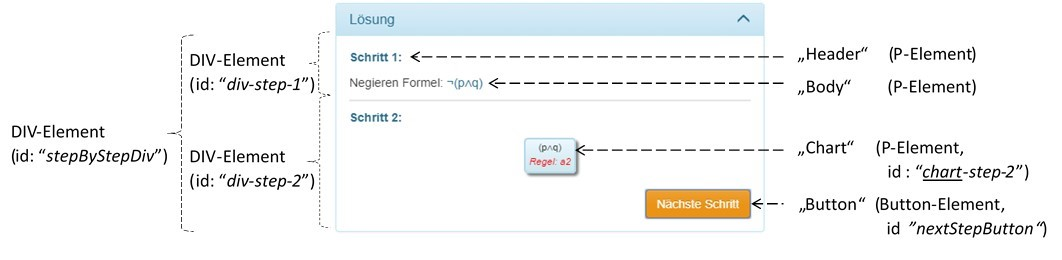
\includegraphics[width=1.0\textwidth]{StepByStepPanelAufbau}
\caption[Aufbau der StepByStepPanel]{Aufbau der ``Schritt für Schritt Lösung'' Panel}\label{fig:StepByStepPanelAufbau}
\end{figure}

Das Konzept für die ``Schritt für Schritt Lösung'' ist es, dass zuerst die vollständige Lösung mit allen Schritten erstellt und je nach Bestätigung der ``Nächste Schritt'' Button wird die Lösung teilweise eingeblendet.

\subsection{Controller}\label{subsec:Controller}

Controller (Klasse \textit{TableauController}) sind verantwortlich für die Steuerung der Anwendung durch den Benutzer und dieser wird für die Kommunikation zwischen den Model und View verwendet. Sie werten die Eingabedaten aus und leiten sie weiter. Änderungen der Modelldaten werden also vom Controller eingeleitet. View und Controller bilden zusammen die Benutzungsoberfläche. Das Klassendiagramm der \textit{TableauController} ist in Abbildung \ref{fig:KlassendiagrammControllerView} gezeigt.

\begin{lstlisting}[language=JavaScript, caption= TableauController Konstruktor, basicstyle=\scriptsize] 
function TableauController(TableauView) {
    this.view = TableauView;
    this.rootFormula = this.getRootOfParserTree(this.view.input.value);
    this.tableau = null;
    this.rootTableau = null;
    if (!InputError) {
        this.tableau = new TableauForPropositionalLogic(this.rootFormula);
        this.rootTableau = this.tableau.rootNode;
    }
    return this;
}
\end{lstlisting}

Im Konstruktor des Controllers wird zunächst seine Methode \textit{getRootOfParserTree()} aufgerufen. Diese Methode erhält die Eingabe, die im Attribut \textit{input} der \textit{TableauView} gekapselt wird, und führt die generierten Lexer und Parser aus um einen Parse-tree zu erhalten. Mit Hilfe von einer Instanz der Klasse  \textit{FormulaListener} besucht sie diesen Parse-tree, um eine Baumdarstellung der Eingabeformel zu erstellen. Dieser Baum wird im Attribut \textit{rootFormula} des Controller gespeichert. Danach wird eine Instanz der Klasse \textit{TableauForPropositionalLogic} initialisiert, um ein Tableau der Eingabeformel zu erstellen. Die Wurzel des Tableau wird im Attribut \textit{rootTableau} des Controller gespeichert.

\begin{lstlisting}[language=JavaScript, caption=getRootOfParserTree() (Klasse TableauController), basicstyle=\scriptsize] 
TableauController.prototype.getRootOfParserTree = function (inputString) {
    var errorListener = new ErrorListener();
    var chars = new antlr4.InputStream(inputString);
    var lexer = new FormulaGrammarLexer(chars);
    var tokens = new antlr4.CommonTokenStream(lexer);
    var parser = new FormulaGrammarParser(tokens);
    parser.buildParseTrees = true;
    var tree = parser.stat();
    var listener = new FormulaListener();
    antlr4.tree.ParseTreeWalker.DEFAULT.walk(listener, tree);
    var root = listener.stack.slice(-1).pop();
    return root;
};
\end{lstlisting}

Wenn der Anwender den Button ``Erfüllbarkeit'' betätigt, wird die Methode \textit{satisfiable()} des Controllers ausgeführt. Die Methode wird zuerst die Eingabeformel mittels Google Charts darstellen und die Panels der View einblenden und das Prüfergebnis, das man mittels Methode \textit{isSatisfiable()} der Klasse \textit{TableauForPropositionalLogic} erhält, in der GUI ausgeben. Anschließend wird sie die  Tableau-Darstellung einblenden. Abschließend, mit Hilfe der Methoden \textit{createSolutionStepHeaderP()}, \textit{createSolutionStepBodyP(}) der Klasse TableauView wird sie die ``Schritt für Schritt Lösung'' erstellen.

Wenn der Anwender den Button ``Tautologie'' betätigt, wird die Methode \textit{tautology()} des Controllers ausgeführt. Diese Methode analog zur Methode \textit{satisfiable()}, dann wird sie zuerst die Eingabeformel negieren und das Attribut \textit{rootFormula} mit der Negationsformel aktualisieren. Danach prüft sie die Erfüllbarkeit der negierten Formel und die Ergebnisse werden eingeblendet.
\begin{lstlisting}[language=JavaScript, caption=tautology() (Klasse TableauController), basicstyle=\scriptsize] 
TableauController.prototype.tautology = function () {
    // this.rootFormula = this.getRootOfParserTree(this.view.input.value);
    google.charts.setOnLoadCallback(drawFormulaChart);
    this.view.panelFormula.style.display = 'block';
    var formula = this.rootFormula.toFormulaString();
    this.rootFormula = this.rootFormula.getNegativeFormula();
    this.tableau = new TableauForPropositionalLogic(this.rootFormula);
    this.rootTableau = this.tableau.rootNode;
    this.view.panelResult.style.display = 'block';
    this.view.tautologyDiv.style.display = 'block';
    this.view.unsatisfiableDiv.style.display = 'none';
    this.view.satisfiableDiv.style.display = 'none';
    if (this.tableau.isSatisfiable()) {
        isTautology = TautologyOrSatisfiableEnum.FALSE;
        isSatifiable = TautologyOrSatisfiableEnum.NOTTESTED;
        this.view.tautologySpan.innerHTML = formula + " ist keine ";
    } else {
        isTautology = TautologyOrSatisfiableEnum.TRUE;
        isSatifiable = TautologyOrSatisfiableEnum.NOTTESTED;
        this.view.tautologySpan.innerHTML = formula + " ist eine ";
    }
    this.view.formula.innerHTML = "Negierte Formel: ";
    this.view.tableau.innerHTML = "Tableau der negierten Formel: ";
    this.view.panelTableau.style.display = 'block';
    google.charts.setOnLoadCallback(drawTableauChart);
    this.view.createSolutionStepHeaderP(this.view.stepByStepDiv);
    var text = "Negieren Formel:  <span  class='text-info'>" + this.rootFormula.toFormulaString() + "</span>";
    this.view.createSolutionStepBodyP(this.view.stepByStepDiv, text);
    chartNr = 2;
    stepNr++;
};
\end{lstlisting}

Weiterhin bietet die Klasse \textit{TableauController} noch die Methode \textit{toDisplayInput()}. Mit Hilfe des Lexers von ANTLR formatiert die Methode die Eingabeformel (z.B von p\&q nach p$\wedge$q). Diese formatierende Formel wird mittels der Klassen \textit{TableauView} eingeblendet.	
%\cleardoublepage
\chapter{Softwaretest}\label{sec:Softwaretest}
Der Softwaretest umfasst eine Nachweisstrategie und die Vorgaben der Entwicklung, um eine hochwertige Anwendung zu erstellen.

Die Nachweisstrategie beschreibt die Anwendung von Unit-Test auf das Gesamtsystem, insbesondere die Festlegung des Einsatzes und das Code Coverage.

Vorgaben für die Entwicklungsumgebung umfasst die Konfiguration der Unit-Tests/ Code Coverage Tools und die Verwendung der Testergebnisse.

\section{Konzept zum Softwaretest}
Das Konzept umfasst das Testverfahren während der Entwicklung mit abschließender Testdokumentation.

Folgende Anforderungen stellt das Konzept an das Testverfahren
\begin{itemize}
\item	Jede Methode wird mit Unit-Tests getestet. 
\item	Die Unit-Tests werden begleitend zur Entwicklungsphase geschrieben und erweitert
\item	Abschließend decken die Unit-Tests mindestens 85\% der implementierten Methoden ab, Frameworks ausgenommen
\item 	Regelmäßiges Prüfen der Code Coverage
\end{itemize}

Während des Entwicklungsprozesses wurden die Unit-Test kontinuierlich vervollständigt und mittels Code Coverage geprüft, ob die Testabdeckung ausreichend ist.

Die Unit-Tests wurden mit Hilfe von Jasmine erstellt.  Mittels zwei HTML-Dateien  \textit{``UnitTestModel.html''} und \textit{``UnitTestControllerView.html''} werden die Tests integriert. Darin erhält \textit{``UnitTestModel.html''} die Tests für das Model. Und \textit{``UnitTestControllerView.html''} enthält die Tests für den Controller und die View sowie einer Kopie der \textit{indexTableau.html} Dateien um die Manipulation des DOM-Tree zu testen. In der Datei \textit{``UnitTestModel.html''} wird das Test-Framework Jasmine im head-Tag eingebunden (Listing \ref{lis:EinbildungModel}). Dagegen wird Jasmine in der Datei \textit{``UnitTestControllerView.html''} am Ende der Seite im  body-Tag eingebunden, da es notwendig ist, dass das Markup vollständig geladen ist, bevor mit den Test begonnen werden kann (Listing \ref{lis:EinbildungControllerView}).
\begin{lstlisting}[language=HTML, caption= Einbildung Jasmine und Test-Dateien (Model), label=lis:EinbildungModel,basicstyle=\scriptsize]
<script src="lib/jasmine-3.1.0/jasmine.js"></script>
[...]
    <script src="lib/jasmine-3.1.0/jasmine-html.js"></script>
    <script src="lib/jasmine-3.1.0/boot.js"></script>

    <!--incl. Test files here...-->
    <script src="Tests/FormulaListenerUnitTest.js"></script>
    <script src="Tests/FormulaUnitTest.js"></script>
    <script src="Tests/TableauNodeUnitTest.js"></script>
    <script src="Tests/TableauForPropositionalLogicUnitTest.js"></script>
</head>
<body>
</body>
</html>
\end{lstlisting}

\begin{lstlisting} [language=HTML, caption= Einbildung Jasmine und Test-Dateien (Controller und View),label=lis:EinbildungControllerView, basicstyle=\scriptsize]
[...]
<!--incl. Test files here...-->
<script src="src/Global.js"></script>
<script src="src/TableauClient.js"></script>
<script src="Tests/TableauControllerAndViewUnitTest.js"></script>
</body>
\end{lstlisting}

Der Aufbau von Tests sieht wie folgt aus (Listing \ref{lis:FormulaTest}):

\begin{lstlisting} [language=JavaScript, caption= Beispiel Test der Klasse Formula, label=lis:FormulaTest, basicstyle=\scriptsize]
describe("Unit Tests for Formula", function() {
    var left = new Formula("p", null, null,FormulaTypEnum.POSITIVLITERAL);
    var right = new Formula("p", null ,null,FormulaTypEnum.POSITIVLITERAL);
    var root = new Formula(FormulaOperatorEnum.AND,left,right, FormulaTypEnum.ALPHA);
    var negation =  new Formula(FormulaOperatorEnum.NEG,null,root, FormulaTypEnum.BETA);

    it("p&q has type as ALPHA, p and p have types as POSITIVLITERAL", function() {
        expect(left.getFormulaTyp()).toEqual(FormulaTypEnum.POSITIVLITERAL);
        expect(right.getFormulaTyp()).toEqual(FormulaTypEnum.POSITIVLITERAL);
        expect(root.getFormulaTyp()).toEqual(FormulaTypEnum.ALPHA);

    });
    it("p&q has left child as p and right child as p", function() {
        expect(root.getLeft()).toEqual(left);
        expect(root.getRight()).toEqual(right);
    });

    it("p has negative formula as !p", function() {
        expect(left.getNegativeFormula()).toEqual(new Formula(FormulaOperatorEnum.NEG,null,p,FormulaTypEnum.NEGATIVLITERAL));
    });
	[...]
});
\end{lstlisting}


\section{Evaluation der Testfälle}
Es gibt insgesamt 72 Unit-Tests für das Model (Abbildung \ref{fig:TestResultModel}) und 16 Unit-Tests für den Controller und die View (Abbildung \ref{fig:TestResultControllerView}).

\begin{figure}[ !h] \centering
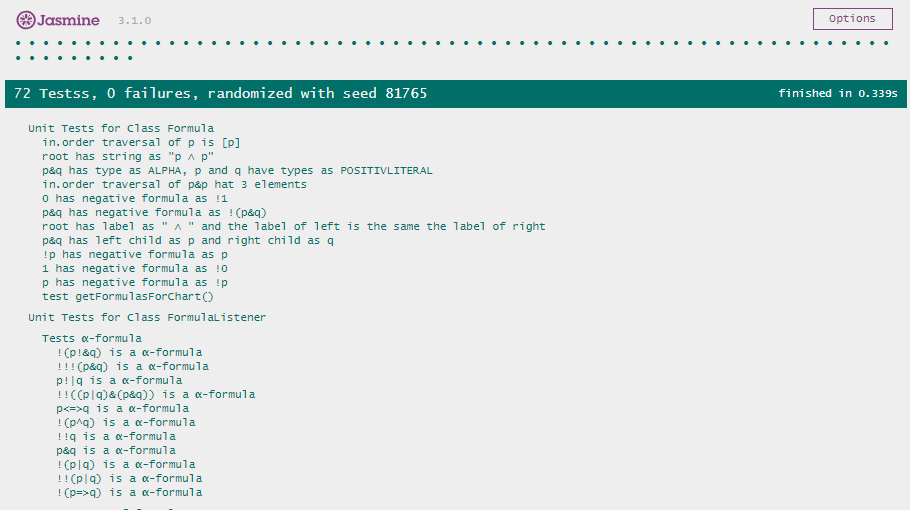
\includegraphics[width=1.0\textwidth]{TestResultModel}
\caption[Testergebnisse des Models]{Ein Teil der Testergebnisse des Models}\label{fig:TestResultModel}
\end{figure}

\begin{figure}[ !h] \centering
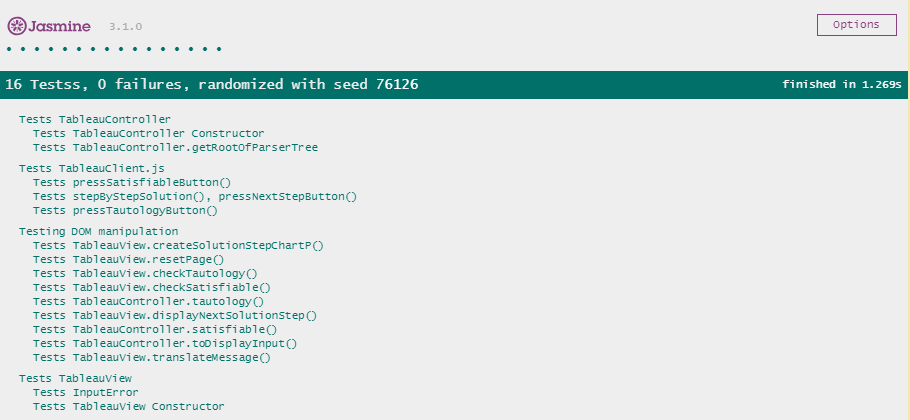
\includegraphics[width=1.0\textwidth]{TestResultControllerView}
\caption[Testergebnisse des Controllers und der View]{Testergebnisse des Controllers und der View}\label{fig:TestResultControllerView}
\end{figure}

Die Tests sind nach der Klasse gruppiert und können dementsprechend zielgerichtet evaluiert werden.
\begin{itemize}

\item \textit{FormulaUnitTest.js}: Enthält 12 Tests für die Klasse \textit{Formula}, wobei alle Methoden der Klasse \textit{Formula} mindestens einmal überprüft werden. Die Methode \textit{getNegativeFormula()} wird mit den Eingabeformeln als Konstante True/False, positive-/negative-Literal, $\alpha $- und  $\beta $-Formel überprüft.

\item \textit{FormulaListenerUnitTest.js}: Enthält 30 Tests. Diese Tests untersuchen die Struktur einer Formel wie linken (\textit{left}) und rechten (\textit{right}) Teilbaum, inhalt (\textit{label}) und Formeltypen (\textit{formulaType}) nachdem sie mithilfe der Klasse \textit{FormulaListener} von Zeichenkette in einen Baum konvertiert wurden. Für jeden Formeltyp (Konstante True/False, positive-/negative-Literal, $ \alpha $- und  $ \beta $-Formel) und für jede Regel der Klassifizierung von $\alpha$- und $\beta$-Formeln wird mindestens eine Formel überprüft.

\item \textit{TableauNodeUnitTest.js}: Enthält 12 Tests für die Klasse \textit{TableauNode}, wobei alle Methoden der Klasse \textit{TableauNode} mindestens einmal überprüft werden. Alle Methoden, die den booleschen Wert zurückgeben, werden mindestens zweimal mit den Rückgabewerten false und true überprüft. Die Methoden \textit{containsOnlyLiterals()}, \textit{containsAComplementaryPairOfLiterals()} und \textit{containsAlphaFormula()} werden mit den Tableau-Knoten, die mit der Menge von Formeln $\{q\}$, $\{p\wedge(q\vee\neg p)\}$, $\{p,q\}$, $\{p,\neg p\}$, $\{\neg p,p\}$, $ \{p,q\vee\neg p\} $, $\{p,\neg p,\neg\neg p\}$, $\{p,1\}$ und $\{q,0\}$ markiert sind, getestet.

\item \textit{TableauForPropositionalLogicUnitTest.js}: Enthält 18 Tests für die Klasse \textit{TableauForPropositionalLogic}, wobei alle Methoden der Klasse \textit{TableauForPropositionalLogic} mindestens einmal überprüft werden. Die Methoden \textit {determineAlphaFormulas()} und \textit{determineBetaFormulas()} werden für jede Regel der Klassifizierung von $\alpha$- und $\beta$-Formeln mindestens einmal überprüft.

\item \textit{TableauControllerandViewUnitTest.js}: Enthält 16 Tests für die Klassen \textit{TableauView}, \textit{TableauController}, \textit{TableauClient.js} und \textit{TableauClient.js} wobei alle Methoden mindestens einmal überprüft werden. Die Methoden \textit { pressSatisfiableButton()} und \textit{pressTautologyButton()} werden für eine syntaktisch korrekte Formel und eine fehlerhafte Formel einmal überprüft.
\end{itemize}


\section{Code Coverage}

\begin{figure}[ !h] \centering
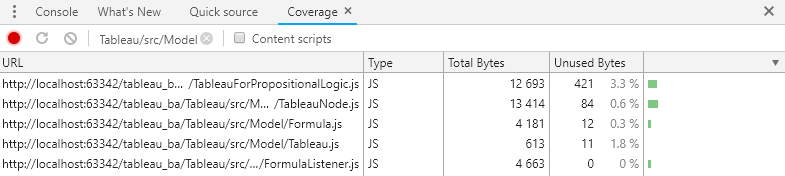
\includegraphics[width=1.0\textwidth]{TestCoverageModel2}
\caption[Code Coverages des Models]{Code Coverages des Models}\label{fig:TestCoverageModel}
\end{figure}

\begin{figure}[ !h] \centering
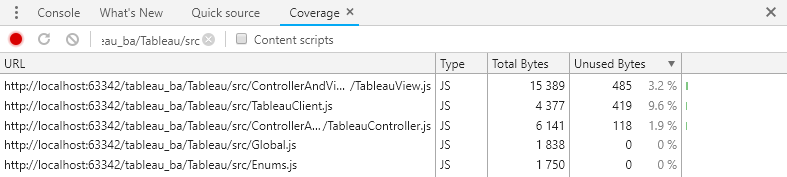
\includegraphics[width=1.0\textwidth]{TestCoverageControllerView5}
\caption[Code Coverages des Controllers und der View]{Code Coverages des Controllers und der View}\label{fig:TestCoverageClientLogik}
\end{figure}

Um eine Code Coverage zu messen, ist ein weiteres Tool notwendig. Es gibt dafür Chrome DevTools, das besteht aus einer Reihe von Webentwicklungs-Tools, die direkt in den Google Chrome-Browser integriert sind. Die neueste DevTools Version (Chrome 59) bietet eine neue Registerkarte ``Coverage'' an. Wenn man eine Seite lädt oder ausführt, erfährt man auf dieser Registerkarte, wie viel Prozent des heruntergeladenen Codes, noch nicht verwendet wurde \cite{Kayce}.
Die Ergebnisse der Codeabdeckung sind unter den Abbildungen \ref{fig:TestCoverageModel} und \ref{fig:TestCoverageClientLogik} zu sehen.

Alle Dateien erfüllen die Mindestgrenze unter Rücksichtnahme, dass das Tool bei \textit{switch-case} und \textit{if-clause}(ohne \textit{else}) nicht richtig ausgewertet werden konnte. Außerdem konnte das Tool auch nicht jedes Event des GUI mit auswerten, deshalb kommt es zu verfälschten Ergebnissen (Abbildung \ref{fig:FehlerCoverage}).

\begin{figure}[ !h] \centering
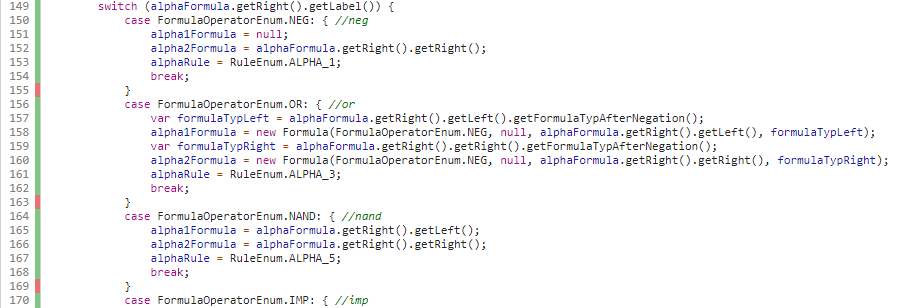
\includegraphics[width=1.0\textwidth]{FehlerCoverage}
\caption[Problem bei CodeCoverages]{Problem bei Code Coverages}
\label{fig:FehlerCoverage}
\end{figure}
%\cleardoublepage
\chapter{Zusammenfassung}
Diese Arbeit hat die beschriebenen Anforderungen erfüllt. Die Kernaufgabe besteht darin, eine Webanwendung für ein semantisches Tableau zu entwickeln, um ermitteln zu können, ob eine Formel erfüllbar oder allgemeingültig ist. Darüber hinaus kann die Anwendung die Struktur von einem Tableau über Google Chart Tools visualisieren. Zur Unterstützung bei dem Erlernen der Konstruktion eines semantischen Tableaus bietet die Anwendung auch eine ``Schritt für Schritt Lösung'' -Funktion, wonach Studierende Schritt für Schritt den Aufbau eines Tableaus folgen können. Nicht nur das, die Anwendung wurde entwickelt, um eine Vielzahl von Geräten von Desktop bis Smartphone zu unterstützen.

Es wäre ideal, wenn die Anwendung in Zukunft weiterentwickelt  werden könnte, zum Beispiel: Unterstützung für die prädikatenlogischen Formeln oder Verwendung eines Offline-Frameworks, um ein Tableau ohne Internetverbindung visualisieren zu können.


\clearpage
\pagestyle{empty} % Seitennummerierung abschalten
\input{danksagung} % optional
\cleardoublepage

% ---------------------------------------------------------------
\backmatter % ab hier keine Nummerierung mehr
 \pagestyle{empty} % Seitennummerierung abschalten
	\listoffigures
	\listoftables
	\printglossaries %hiermit würde der Glossar dargestellt
    %\bibliographystyle{geralpha} %alte Befehle ohne biber
    %\bibliography{./bib/thesis}
	%\printbibliography
%\bibliographystyle{plain}
\bibliographystyle{alphadin} %alte Befehle ohne biber
\thispagestyle{empty}
\bibliography{bib}
\end{document}



